%Casos de uso%
\section{Casos de uso}
Los casos de uso que describen el funcionamiento del prototipo se muestran en la figura 3.1 Casos de uso del editor, los casos de uso se dividieron por módulos para organizar de una mejor manera la visualización y el desarrollo. Los módulos que conforman el editor son:

\begin{itemize}
	\item Administrador
	\item Líder de Análisis
	\item Módulos
	\item Casos de Uso
	\item Pantallas
	\item Entidades
	\item Reglas de Negocio
	\item Mensajes
	\item Actores
	\item Términos del Glosario
\end{itemize}
\newpage
En el diagrama \ref{fig:CasosUsoTesseract} se marcan los casos de uso clave para el editor y en las siguientes secciones se describe cada uno de ellos.

	\begin{figure}[H]
		\begin{center}
			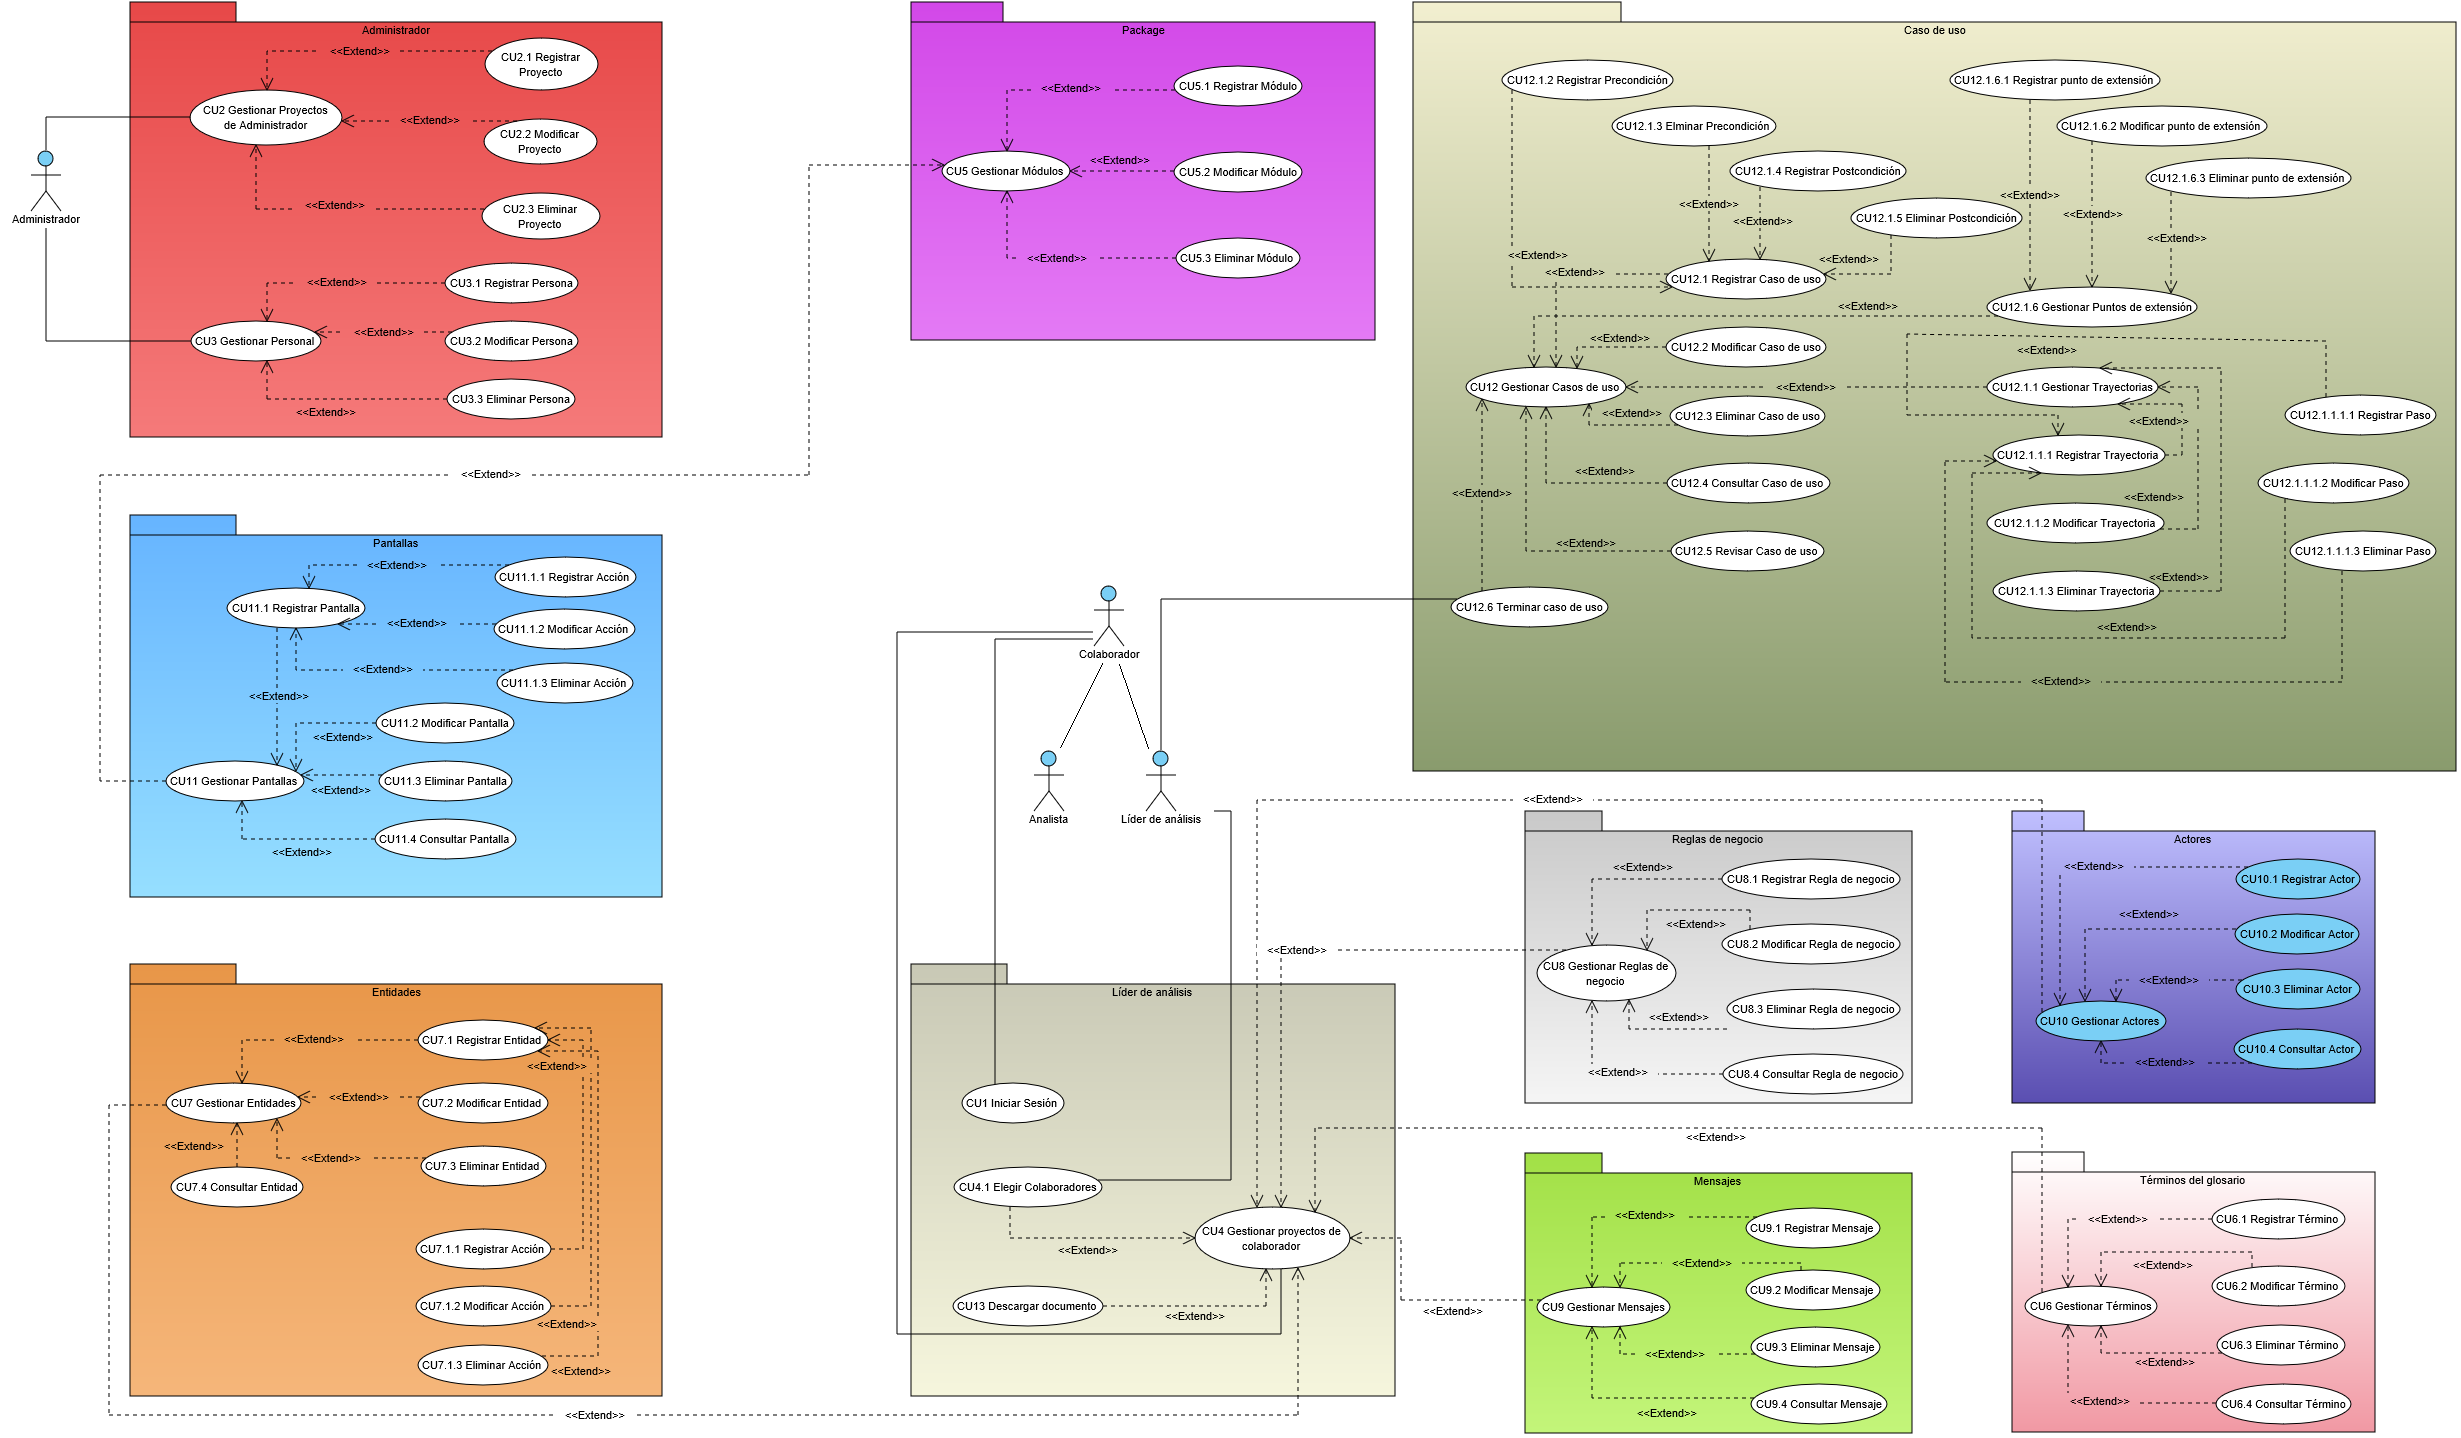
\includegraphics[angle=0,width=.95\textwidth]{images/CasosUsoTesseract}
			\caption{Casos de uso del editor}
			\label{fig:CasosUsoTesseract}
		\end{center}
	\end{figure}
\newpage

La figura \ref{fig:moduloAdmin} muestra los casos de uso del administrador que incluyen la gestión de proyectos y del personal.

	\begin{figure}[H]
		\begin{center}
			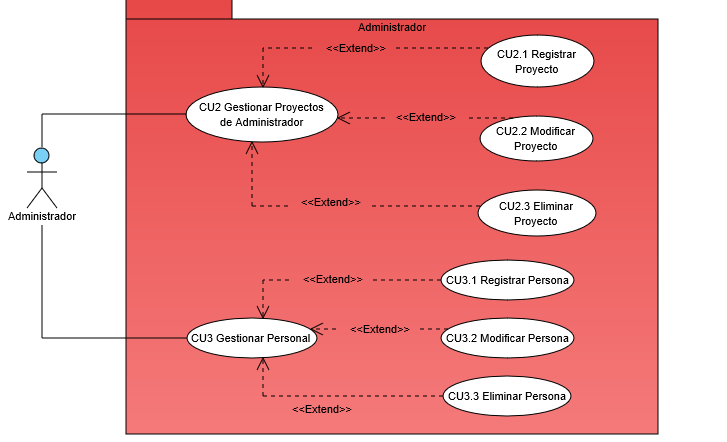
\includegraphics[angle=0,width=.80\textwidth]{images/moduloAdmin}
			\caption{Casos de uso del módulo: Administrador}
			\label{fig:moduloAdmin}
		\end{center}
	\end{figure}
\newpage
La figura \ref{fig:moduloLider} muestra los casos de uso del líder de análisis que incluyen elegir colaboradores y gestionar proyectos.

\begin{figure}[H]
	\begin{center}
		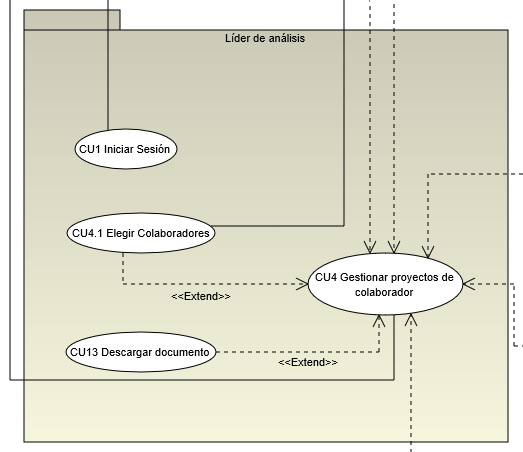
\includegraphics[angle=0,width=.70\textwidth]{images/moduloLider}
		\caption{Casos de uso del módulo: Líder de análisis}
		\label{fig:moduloLider}
	\end{center}
\end{figure}
\newpage
La figura \ref{fig:moduloModulos} muestra los casos de uso referentes a la gestión de los módulos.

\begin{figure}[H]
	\begin{center}
		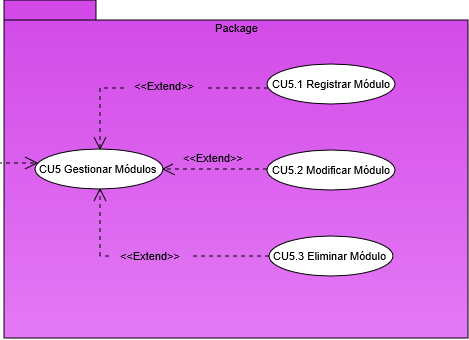
\includegraphics[angle=0,width=.70\textwidth]{images/moduloModulos}
		\caption{Casos de uso del módulo: Módulos}
		\label{fig:moduloModulos}
	\end{center}
\end{figure}
\newpage
La figura \ref{fig:moduloCU} muestra los casos de uso referentes a la gestión de los casos de uso.

\begin{figure}[H]
	\begin{center}
		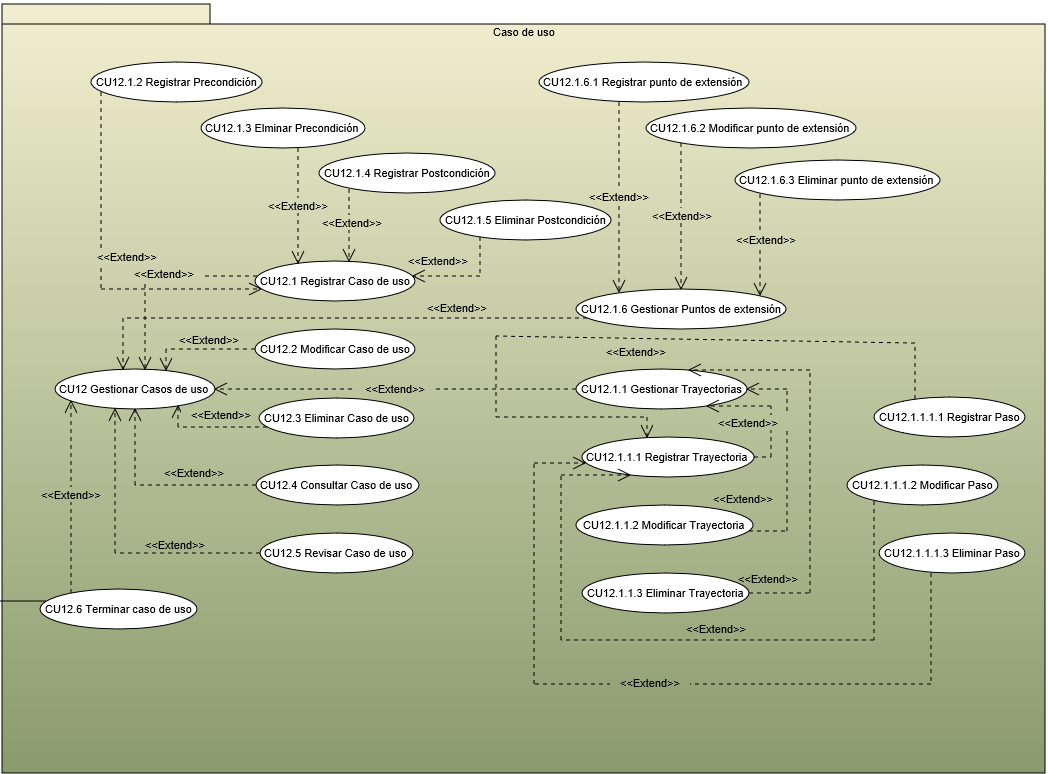
\includegraphics[angle=0,width=.70\textwidth]{images/moduloCU}
		\caption{Casos de uso del módulo: Casos de uso}
		\label{fig:moduloCU}
	\end{center}
\end{figure}
\newpage
La figura \ref{fig:moduloIU} muestra los casos de uso referentes a la gestión de las pantallas y las acciones de estas.

\begin{figure}[H]
	\begin{center}
		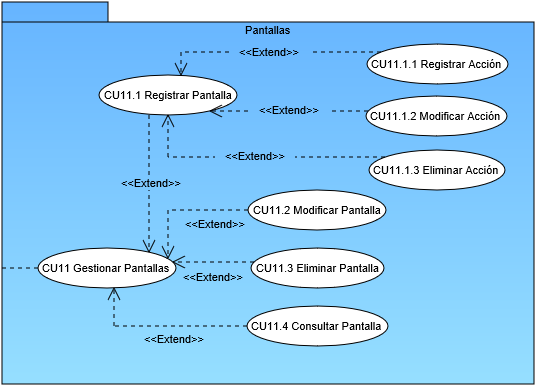
\includegraphics[angle=0,width=.70\textwidth]{images/moduloIU}
		\caption{Casos de uso del módulo: Pantallas}
		\label{fig:moduloIU}
	\end{center}
\end{figure}
\newpage
La figura \ref{fig:moduloEntidades} muestra los casos de uso referentes a la gestión de las entidades y atributos que las describen.

\begin{figure}[H]
	\begin{center}
		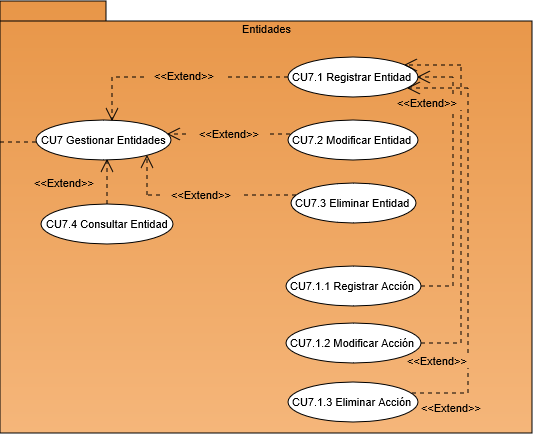
\includegraphics[angle=0,width=.70\textwidth]{images/moduloEntidades}
		\caption{Casos de uso del módulo: Entidades}
		\label{fig:moduloEntidades}
	\end{center}
\end{figure}
\newpage
La figura \ref{fig:moduloBR} muestra los casos de uso referentes a la gestión de las reglas de negocio.

\begin{figure}[H]
	\begin{center}
		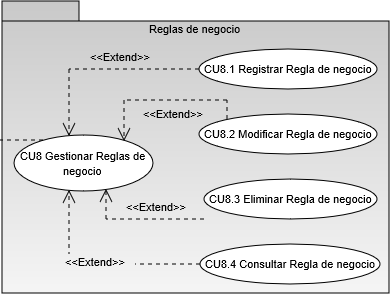
\includegraphics[angle=0,width=.70\textwidth]{images/moduloBR}
		\caption{Casos de uso del módulo: Reglas de negocio}
		\label{fig:moduloBR}
	\end{center}
\end{figure}
\newpage
La figura \ref{fig:moduloMSG} muestra los casos de uso referentes a la gestión de los mensajes.

\begin{figure}[H]
	\begin{center}
		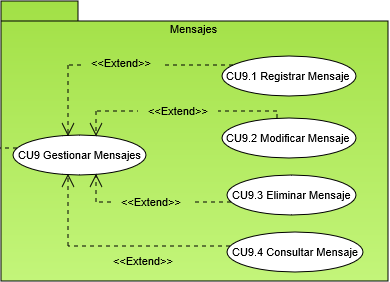
\includegraphics[angle=0,width=.70\textwidth]{images/moduloMSG}
		\caption{Casos de uso del módulo: Mensajes}
		\label{fig:moduloMSG}
	\end{center}
\end{figure}
\newpage
La figura \ref{fig:moduloActores} muestra los casos de uso referentes a la gestión de los Actores.

\begin{figure}[H]
	\begin{center}
		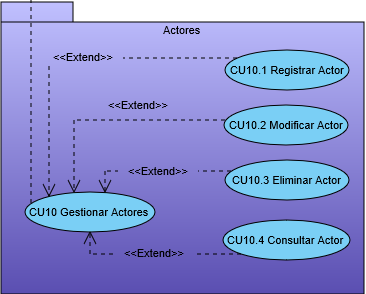
\includegraphics[angle=0,width=.70\textwidth]{images/moduloActores}
		\caption{Casos de uso del módulo: Actores}
		\label{fig:moduloActores}
	\end{center}
\end{figure}
\newpage
La figura \ref{fig:moduloGLS} muestra los casos de uso referentes a la gestión de los términos del glosario.

\begin{figure}[H]
	\begin{center}
		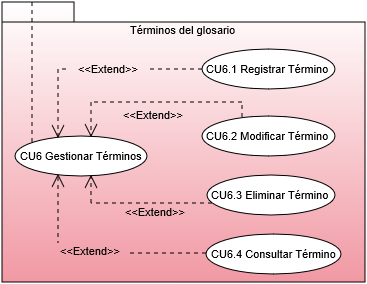
\includegraphics[angle=0,width=.70\textwidth]{images/moduloGLS}
		\caption{Casos de uso del módulo: Términos del glosario}
		\label{fig:moduloGLS}
	\end{center}
\end{figure}

	\begin{UseCase}{CU1}{Iniciar sesión}{
		El actor se ingresa con su nombre y contraseña a su perfil y hacer uso de las funciones que le competen.
	}
		\UCitem{Versión}{\color{Gray}0.1}
		\UCitem{Actor}{\hyperlink{jefe}{Líder de proyecto}, \hyperlink{analista}{Analista}, \hyperlink{admin}{Administrador}}
		\UCitem{Propósito}{Iniciar sesión en el sistema.}
		\UCitem{Entradas}{\begin{itemize}
				\item \cdtRef{colaboradorEntidad:correoColaborador}{Correo}: Se escribe desde el teclado
				\item \cdtRef{colaboradorEntidad:passColaborador}{Contraseña}: Se escribe desde el teclado
		\end{itemize}}
		\UCitem{Salidas}{Ninguna}
		\UCitem{Destino}{Pantalla}
		\UCitem{Precondiciones}{Que el actor se encuentre registrado en el sistema.}
		\UCitem{Postcondiciones}{El actor podrá hacer uso del sistema.}
		\UCitem{Errores}{\begin{itemize}
		\item \cdtIdRef{MSG4}{Dato Obligatorio}: Se muestra en la pantalla \IUref{IU1}{Iniciar Sesión} cuando no se ha ingresado un dato marcado como obligatorio.
		\item \cdtIdRef{MSG6}{Longitud inválida}: Se muestra en la pantalla \IUref{IU1}{Iniciar Sesión} cuando se ha excedido la longitud de alguno de los campos.
		\item \cdtIdRef{MSG23}{Correo electrónico y/o contraseña incorrectos}: Se muestra en la pantalla \IUref{IU1}{Iniciar Sesión} cuando el correo electrónico y/o la contraseña ingresada son incorrectos.
		\item \cdtIdRef{MSG31}{Longitud Mínima}: Se muestra en la pantalla \IUref{IU1}{Iniciar Sesión} cuando se ha ingresado una contraseña que no cumple con la longitud mínima.
		\end{itemize}
		}
		\UCitem{Tipo}{Caso de uso primario}
	\end{UseCase}
%--------------------------------------
	\begin{UCtrayectoria}
		\UCpaso[\UCactor] Solicita ingresar al sistema a través de la URL.
		\UCpaso[\UCsist] Muestra la pantalla \IUref{IU1}{Iniciar Sesión}.
		\UCpaso[\UCactor] Ingresa los datos solicitados. \label{P3}
		\UCpaso[\UCactor] Oprime el botón \IUbutton{Aceptar}.
		\UCpaso[\UCsist] Verifica que no se haya omitido ningún campo marcado como obligatorio con base en la regla de negocio \BRref{RN8}{Datos Obligatorios}. \hyperlink{CU1:TAA}{[Trayectoria alternativa A]}
		\UCpaso[\UCsist] Verifica que los datos cumplan con el formato y el tipo de dato requerido, con base en la regla de negocio \BRref{RN7}{Información correcta}. \Trayref{B} \Trayref{C} \Trayref{D}
		\UCpaso[\UCsist] Verifica que el actor se encuentre registrado en el sistema. \Trayref{E}
		\UCpaso[\UCsist] Verifica que la contraseña ingresada corresponda con la del usuario. \Trayref{E}
		\UCpaso[\UCsist] Muestra la pantalla IU 4 Gestionar proyectos.	
	\end{UCtrayectoria}		
%--------------------------------------
		\hypertarget{CU1:TAA}{\textbf{Trayectoria alternativa A}}\\
		\noindent \textbf{Condición:} El actor no ingresó uno o más campos obligatorios
		\begin{enumerate}
			\UCpaso[\UCsist] Muestra el mensaje \cdtIdRef{MSG4}{Dato Obligatorio} y señala el campo que presenta el error en la pantalla \IUref{IU1}{Iniciar Sesión}.
			\UCpaso[\UCactor] Regresa al paso \ref{P3} de la Trayectoria Principal.
			\item[- -] - - {\em {Fin de la trayectoria}}.%
		\end{enumerate}

%--------------------------------------
		\begin{UCtrayectoriaA}{B}{El actor ingresó un dato con un número de caracteres fuera del rango permitido}
	\UCpaso[\UCsist] Muestra el \cdtIdRef{MSG6}{Longitud inválida} y señala el campo que presenta el error en la pantalla \IUref{IU1}{Iniciar Sesión}.
	\UCpaso[\UCactor] Regresa al paso \ref{P3} de la Trayectoria Principal.
\end{UCtrayectoriaA}

	\begin{UCtrayectoriaA}{C}{El actor ingresó un tipo de dato incorrecto.}
		\UCpaso[\UCsist] Muestra el mensaje \cdtIdRef{MSG29}{Formato incorrecto} y señala el campo que presenta el dato inválido en la pantalla \IUref{IU1}{Iniciar sesión}, para indicar que se ha ingresado un tipo de dato inválido.
		\UCpaso Regresa al paso \ref{P3} de la trayectoria principal.
	\end{UCtrayectoriaA}

	\begin{UCtrayectoriaA}{D}{El actor ingresó una contraseña que no cumple la longitud mínima requerida}
		\UCpaso[\UCsist] Muestra el mensaje \cdtIdRef{MSG31}{Longitud mínima} y señala el campo que presenta el dato inválido en la pantalla \IUref{IU1}{Iniciar sesión}, para indicar que se ha ingresado una contraseña que no cumple con la longitud mínima.
		\UCpaso Regresa al paso \ref{P3} de la trayectoria principal.
	\end{UCtrayectoriaA}
%--------------------------------------
		\begin{UCtrayectoriaA}{E}{El actor ingresó un dato incorrecto}
	\UCpaso[\UCsist] Muestra el mensaje \cdtIdRef{MSG23}{Correo electrónico y/o contraseña incorrectos} en la pantalla \IUref{IU1}{Iniciar Sesión} notificando que los datos ingresados son incorrectos.
	\UCpaso[\UCactor] Regresa al paso \ref{P3} de la Trayectoria Principal.
\end{UCtrayectoriaA}
	\begin{UseCase}{CU2}{Gestionar proyectos de Administrador}{
		Permite al Administrador visualizar todos los proyectos registrados en el sistema, además sirve como punto de acceso para registrar, modificar o eliminar un proyecto.
	}
		\UCitem{Versión}{\color{Gray}0.1}
		\UCitem{Actor}{\hyperlink{admin}{Administrador}}
		\UCitem{Propósito}{Proporcionar al actor un mecanismo para llevar el control de los proyectos.}
		\UCitem{Entradas}{Ninguna}
		\UCitem{Salidas}{\begin{itemize}
				\item \hyperlink{proyectoEntidad}{Proyecto}: Tabla que muestra la \cdtRef{proyectoEntidad:claveProyecto}{clave}, \cdtRef{proyectoEntidad:nombreProyecto}{nombre} y el \cdtRef{proyectoEntidad:liderProyecto}{Líder de Proyecto} de todos los proyectos existentes.
		\end{itemize}}
		\UCitem{Destino}{Pantalla}
		\UCitem{Precondiciones}{Ninguna}
		\UCitem{Postcondiciones}{Ninguna}
		\UCitem{Errores}{\begin{itemize}
		\item \cdtIdRef{MSG2}{No existe información}: Se muestra en la pantalla \IUref{IU2}{Gestionar proyectos de Administrador} cuando no existen proyectos registrados
		\end{itemize}
		}
		\UCitem{Tipo}{Caso de uso primario}
	\end{UseCase}
%--------------------------------------
	\begin{UCtrayectoria}
		\UCpaso[\UCactor] Solicita gestionar los proyectos presionando la opción ''Proyectos'' del menú \IUref{MN1}{Menú de Administrador}.
		\UCpaso[\UCsist] Busca la información de los proyectos registrados. \hyperlink{CU2:TAA}{[Trayectoria A]}
		\UCpaso[\UCsist] Muestra la información de los proyectos en la pantalla \IUref{IU2}{Gestionar proyectos de Administrador}.
		\UCpaso[\UCactor] Gestiona los proyectos a través de los botones: \IUbutton{Registrar}, \editar  y \eliminar. \label{P4}
	\end{UCtrayectoria}		
%--------------------------------------
	\hypertarget{CU2:TAA}{\textbf{Trayectoria alternativa A}}\\
\noindent \textbf{Condición:} No existen registros de proyectos.
\begin{enumerate}
	\UCpaso[\UCsist] Muestra el mensaje \cdtIdRef{MSG2}{No existe información} en la pantalla \IUref{IU2}{Gestionar proyectos de Administrador} para indicar que no hay registros de proyectos para mostrar.
	\item[- -] - - {\em {Fin de la trayectoria}}.%
\end{enumerate}
%--------------------------------------

\subsubsection{Puntos de extensión}

\UCExtenssionPoint{El actor requiere registrar un proyecto.}{Paso \ref{P4} de la trayectoria principal.}{\UCref{CU2.1}{Registrar Proyecto}}
\UCExtenssionPoint{El actor requiere modificar un proyecto.}{Paso \ref{P4} de la trayectoria principal.}{\UCref{CU2.2}{Modificar Proyecto}}
\UCExtenssionPoint{El actor requiere eliminar un proyecto.}{Paso \ref{P4} de la trayectoria principal.}{\UCref{CU2.3}{Eliminar Proyecto}}

	\begin{UseCase}{CU2.1}{Registrar proyecto}{
		Este caso de uso permite al actor registrar la información de un proyecto en el sistema.
	}
		\UCitem{Versión}{\color{Gray}0.1}
		\UCitem{Actor}{\hyperlink{admin}{Administrador}}
		\UCitem{Propósito}{Registrar la información de un proyecto.}
		\UCitem{Entradas}{
		\begin{itemize}
			\item \cdtRef{proyectoEntidad:claveProyecto}{Clave:} Se escribe desde el teclado.
			\item \cdtRef{proyectoEntidad:nombreProyecto}{Nombre:} Se escribe desde el teclado.
			\item \cdtRef{proyectoEntidad:fechaIProyecto}{Fecha de inicio:} Se selecciona de un calendario.
			\item \cdtRef{proyectoEntidad:fechaFinProyecto}{Fecha de término:} Se selecciona de un calendario.
			\item \cdtRef{proyectoEntidad:fechaIPProyecto}{Fecha de inicio programada:} Se selecciona de un calendario.
			\item \cdtRef{proyectoEntidad:fechaFinPProyecto}{Fecha de término programada:} Se selecciona de un calendario.
			\item \cdtRef{proyectoEntidad:liderProyecto}{Líder del Proyecto:} Se selecciona de una lista.
			\item \cdtRef{proyectoEntidad:descripcionProyecto}{Descripción:} Se escribe desde el teclado.
			\item \cdtRef{proyectoEntidad:contraparteProyecto}{Contraparte} Se escribe desde el teclado.
			\item \cdtRef{proyectoEntidad:presupuestoProyecto}{Presupuesto:} Se escribe desde el teclado.
			\item \hyperlink{tEdoProy}{Estado del Proyecto:} Se selecciona de un lista.
		\end{itemize}	
		}
		\UCitem{Salidas}{\begin{itemize}
				\item \cdtIdRef{MSG1}{Operación exitosa}: Se muestra en la pantalla \IUref{IU2}{Gestionar proyectos de Administrador} para indicar que el registro fue exitoso.
		\end{itemize}}
		\UCitem{Destino}{Pantalla}
		\UCitem{Precondiciones}{
		\begin{itemize}
			\item Interna: Que exista al menos un colaborador registrado.
			\item Interna: Que exista información referente a los estados del proyecto.
		\end{itemize}
		}
		\UCitem{Postcondiciones}{
		\begin{itemize}
			\item Se registrará un proyecto en el sistema.
			\item Interna: Se podrán gestionar los Términos del glosario, Entidades, Reglas de negocio, Mensajes y Actores.
		\end{itemize}
		}
		\UCitem{Errores}{\begin{itemize}
		\item \cdtIdRef{MSG4}{Dato obligatorio}: Se muestra en la pantalla \IUref{IU2.1}{Registrar proyecto} cuando no se ha ingresado un dato marcado como obligatorio.
		\item \cdtIdRef{MSG29}{Formato incorrecto}: Se muestra en la pantalla \IUref{IU2.1}{Registrar proyecto} cuando el tipo de dato ingresado no cumple con el tipo de dato solicitado en
		el campo.
		\item \cdtIdRef{MSG6}{Longitud inválida}: Se muestra en la pantalla \IUref{IU2.1}{Registrar proyecto} cuando se ha excedido la longitud de alguno de los campos.
		\item \cdtIdRef{MSG7}{Registro repetido}: Se muestra en la pantalla \IUref{IU2.1}{Registrar proyecto} cuando se registre un proyecto con un nombre o clave que ya se encuentra registrado en el sistema.
		\item \cdtIdRef{MSG12}{Ha ocurrido un error}: Se muestra en la pantalla \IUref{IU2}{Gestionar proyectos de Administrador} cuando no exista información de los estados de un proyecto.
		\item \cdtIdRef{MSG17}{Falta información}: Se muestra en la pantalla \IUref{IU2}{Gestionar proyectos de Administrador} cuando no existan colaboradores registrados.
		\item \cdtIdRef{MSG26}{Orden de fechas}: Se muestra en la pantalla \IUref{IU2.1}{Registrar proyecto} cuando el actor ingrese fechas de término que no son posteriores a las fechas
		de inicio correspondientes.
		\end{itemize}
		}
		\UCitem{Tipo}{Secundario, extiende del caso de uso \UCref{CU2}{Gestionar proyectos de Administrador}.}
	\end{UseCase}
%--------------------------------------
	\begin{UCtrayectoria}
		\UCpaso[\UCactor] Solicita registrar un proyecto oprimiendo el botón \IUbutton{Registrar} de la pantalla \IUref{IU2}{Gestionar proyectos de Administrador}.
		\UCpaso[\UCsist] Verifica que exista información referente a los estados de un proyecto, con base en la regla de negocio \BRref{RN20}{Verificación de catálogos}. \hyperlink{CU2-1:TAA}{[Trayectoria A]}
		\UCpaso[\UCsist] Verifica que exista al menos un colaborador, con base en la regla de negocio \BRref{RN20}{Verificación de catálogos}. \hyperlink{CU2-1:TAB}{[Trayectoria B]}
		\UCpaso[\UCsist] Muestra la pantalla \IUref{IU2.1}{Registrar proyecto}.
		\UCpaso[\UCactor] Ingresa la información solicitada en la pantalla. \label{CU2.1-P5}
		\UCpaso[\UCactor] Solicita guardar el proyecto oprimiendo el botón \IUbutton{Aceptar} de la pantalla \IUref{IU2.1}{Registrar proyecto}. \hyperlink{CU2-1:TAC}{[Trayectoria C]}
		\UCpaso[\UCsist] Verifica que el actor ingrese todos los campos obligatorios con base en la regla de negocio \BRref{RN8}{Datos obligatorios}. \hyperlink{CU2-1:TAD}{[Trayectoria D]}
		\UCpaso[\UCsist] Verificar que los datos ingresados cumpla con la longitud correcta, con base en la regla de negocio \BRref{RN37}{Longitud de datos}. \hyperlink{CU2-1:TAE}{[Trayectoria E]}
		\UCpaso[\UCsist] Verifica que los datos ingresados cumplan con el formato requerido, con base en la regla de negocio \BRref{RN7}{Información correcta}. \hyperlink{CU2-1:TAF}{[Trayectoria F]}
		\UCpaso[\UCsist] Verifica que la clave del proyecto no se encuentre registrada en el sistema con base en la regla de negocio \BRref{RN22}{Unicidad de la clave del Proyecto}. \hyperlink{CU2-1:TAG}{[Trayectoria G]}
		\UCpaso[\UCsist] Verifica que el nombre del proyecto no se encuentre registrado en el sistema con base en la regla de negocio \BRref{RN6}{Unicidad de nombres}. \hyperlink{CU2-1:TAH}{[Trayectoria H]}
		\UCpaso[\UCsist] Verifica que la fecha de término programada sea posterior a la fecha de inicio programada con base en la regla de negocio \BRref{RN35}{Validar Fecha}. \hyperlink{CU2-1:TAI}{[Trayectoria I]}
		\UCpaso[\UCsist] Registra la información del proyecto en el sistema
		\UCpaso[\UCsist] Muestra el mensaje \cdtIdRef{MSG1}{Operación exitosa} en la pantalla \IUref{IU2}{Gestionar proyectos de Administrador} para indicar al actor que el registro se ha realizado exitosamente.
	\end{UCtrayectoria}		
%--------------------------------------
\hypertarget{CU2-1:TAA}{\textbf{Trayectoria alternativa A}}\\
\noindent \textbf{Condición:} El catálogo de estados de un proyecto no tiene información.
\begin{enumerate}
	\UCpaso[\UCsist] Muestra el mensaje \cdtIdRef{MSG12}{Ha ocurrido un error} en la pantalla \IUref{IU2}{Gestionar proyectos de Administrador} para indicar que no es posible realizar la operación debido a la falta de información necesaria para el sistema.
	\item[- -] - - {\em {Fin del caso de uso}}.%
\end{enumerate}

%--------------------------------------
	\hypertarget{CU2-1:TAB}{\textbf{Trayectoria alternativa B}}\\
	\noindent \textbf{Condición:} No hay ningún colaborador registrado.
	\begin{enumerate}
		\UCpaso[\UCsist] Muestra el mensaje \cdtIdRef{MSG12}{Ha ocurrido un error} en la pantalla \IUref{IU2}{Gestionar proyectos de Administrador} para indicar que no es posible realizar la operación debido a la falta de información necesaria para el sistema.
		\item[- -] - - {\em {Fin del caso de uso}}.%
	\end{enumerate}
	
%--------------------------------------
\hypertarget{CU2-1:TAC}{\textbf{Trayectoria alternativa C}}\\
\noindent \textbf{Condición:} El actor desea cancelar la operación.
\begin{enumerate}
	\UCpaso[\UCactor] Solicita cancelar la operación oprimiendo el botón \IUbutton{Cancelar} de la pantalla \IUref{IU2.1}{Registrar Proyecto}
	\UCpaso[\UCsist] Muestra la pantalla \IUref{IU2}{Gestionar proyectos de Administrador}.
	\item[- -] - - {\em {Fin del caso de uso}}.%
\end{enumerate}
%--------------------------------------	
\hypertarget{CU2-1:TAD}{\textbf{Trayectoria alternativa D}}\\
\noindent \textbf{Condición:} El actor no ingresó algún dato marcado como obligatorio.
\begin{enumerate}
	\UCpaso[\UCsist] Muestra el mensaje \cdtIdRef{MSG4}{Dato obligatorio} señalando el campo que presenta el error en la pantalla \IUref{IU2.1}{Registrar Proyecto}.
	\UCpaso Regresa al paso \ref{CU2.1-P5} de la trayectoria principal.
	\item[- -] - - {\em {Fin de la trayectoria}}.%
\end{enumerate}
%--------------------------------------
\hypertarget{CU2-1:TAE}{\textbf{Trayectoria alternativa E}}\\
\noindent \textbf{Condición:} El actor ingresó un dato con un número de caracteres fuera del rango permitido.
\begin{enumerate}
	\UCpaso[\UCsist] Muestra el mensaje \cdtIdRef{MSG6}{Longitud inválida} señalando el campo que presenta el error en la pantalla \IUref{IU2.1}{Registrar Proyecto}.
	\UCpaso Regresa al paso \ref{CU2.1-P5} de la trayectoria principal.
	\item[- -] - - {\em {Fin de la trayectoria}}.%
\end{enumerate}
%-------------------------------------
\hypertarget{CU2-1:TAF}{\textbf{Trayectoria alternativa F}}\\
\noindent \textbf{Condición:} El actor ingresó un dato con un formato de dato incorrecto.
\begin{enumerate}
	\UCpaso[\UCsist] Muestra el mensaje \cdtIdRef{MSG29}{Formato incorrecto} señalando el campo que presenta el error en la pantalla \IUref{IU2.1}{Registrar Proyecto}.
	\UCpaso Regresa al paso \ref{CU2.1-P5} de la trayectoria principal.
	\item[- -] - - {\em {Fin de la trayectoria}}.
\end{enumerate}
%--------------------------------------
\hypertarget{CU2-1:TAG}{\textbf{Trayectoria alternativa G}}\\
\noindent \textbf{Condición:} El actor ingresó una clave de proyecto que ya existe dentro del sistema.
\begin{enumerate}
	\UCpaso[\UCsist] Muestra el mensaje \cdtIdRef{MSG7}{Registro repetido} señalando el campo que presenta la duplicidad en la pantalla \IUref{IU2.1}{Registrar Proyecto}.
	\UCpaso Regresa al paso \ref{CU2.1-P5} de la trayectoria principal.
	\item[- -] - - {\em {Fin de la trayectoria}}.
\end{enumerate}
%--------------------------------------	
\hypertarget{CU2-1:TAH}{\textbf{Trayectoria alternativa H}}\\
\noindent \textbf{Condición:} El actor ingresó un nombre de proyecto que ya existe dentro del sistema.
\begin{enumerate}
	\UCpaso[\UCsist] Muestra el mensaje \cdtIdRef{MSG7}{Registro repetido} señalando el campo que presenta la duplicidad en la pantalla \IUref{IU2.1}{Registrar Proyecto}.
	\UCpaso Regresa al paso \ref{CU2.1-P5} de la trayectoria principal.
	\item[- -] - - {\em {Fin de la trayectoria}}.
\end{enumerate}
%--------------------------------------
\hypertarget{CU2-1:TAI}{\textbf{Trayectoria alternativa I}}\\
\noindent \textbf{Condición:} La fecha de termino programada es menor a la fecha de inicio programada.
\begin{enumerate}
	\UCpaso[\UCsist] Muestra el mensaje \cdtIdRef{MSG26}{Orden de fechas} en el campo de fecha de término programada en la pantalla \IUref{IU2.1}{Registrar Proyecto}.
	\UCpaso Regresa al paso \ref{CU2.1-P5} de la trayectoria principal.
	\item[- -] - - {\em {Fin de la trayectoria}}.
\end{enumerate}
	\begin{UseCase}{CU2.2}{Modificar proyecto}{
		Este caso de uso permite al actor modificar la información de un proyecto en el sistema.
	}
		\UCitem{Versión}{\color{Gray}0.1}
		\UCitem{Actor}{\hyperlink{admin}{Administrador}}
		\UCitem{Propósito}{Modicar la información de un proyecto.}
		\UCitem{Entradas}{
		\begin{itemize}
			\item \cdtRef{proyectoEntidad:claveProyecto}{Clave:} Se escribe desde el teclado.
			\item \cdtRef{proyectoEntidad:nombreProyecto}{Nombre:} Se escribe desde el teclado.
			\item \cdtRef{proyectoEntidad:fechaIProyecto}{Fecha de inicio:} Se selecciona de un calendario.
			\item \cdtRef{proyectoEntidad:fechaFinProyecto}{Fecha de término:} Se selecciona de un calendario.
			\item \cdtRef{proyectoEntidad:fechaIPProyecto}{Fecha de inicio programada:} Se selecciona de un calendario.
			\item \cdtRef{proyectoEntidad:fechaFinPProyecto}{Fecha de término programada:} Se selecciona de un calendario.
			\item \cdtRef{proyectoEntidad:liderProyecto}{Líder del Proyecto:} Se selecciona de una lista.
			\item \cdtRef{proyectoEntidad:descripcionProyecto}{Descripción:} Se escribe desde el teclado.
			\item \cdtRef{proyectoEntidad:contraparteProyecto}{Contraparte} Se escribe desde el teclado.
			\item \cdtRef{proyectoEntidad:presupuestoProyecto}{Presupuesto:} Se escribe desde el teclado.
			\item \hyperlink{tEdoProy}{Estado del Proyecto:} Se selecciona de un lista.
		\end{itemize}	
		}
		\UCitem{Salidas}{\begin{itemize}
				\item \cdtRef{proyectoEntidad:claveProyecto}{Clave:} Lo obtiene el sistema.
				\item \cdtRef{proyectoEntidad:nombreProyecto}{Nombre:} Lo obtiene el sistema.
				\item \cdtRef{proyectoEntidad:fechaIProyecto}{Fecha de inicio:} Lo obtiene el sistema.
				\item \cdtRef{proyectoEntidad:fechaFinProyecto}{Fecha de término:} Lo obtiene el sistema.
				\item \cdtRef{proyectoEntidad:fechaIPProyecto}{Fecha de inicio programada:} Lo obtiene el sistema.
				\item \cdtRef{proyectoEntidad:fechaFinPProyecto}{Fecha de término programada:} Lo obtiene el sistema.
				\item \cdtRef{proyectoEntidad:liderProyecto}{Líder del Proyecto:} Lo obtiene el sistema.
				\item \cdtRef{proyectoEntidad:descripcionProyecto}{Descripción:} Lo obtiene el sistema.
				\item \cdtRef{proyectoEntidad:contraparteProyecto}{Contraparte} Lo obtiene el sistema.
				\item \cdtRef{proyectoEntidad:presupuestoProyecto}{Presupuesto:} Lo obtiene el sistema.
				\item \hyperlink{tEdoProy}{Estado del Proyecto:} Lo obtiene el sistema.
				\item \cdtIdRef{MSG1}{Operación exitosa}: Se muestra en la pantalla \IUref{IU2}{Gestionar proyectos de Administrador} para indicar que el registro fue exitoso.
		\end{itemize}}
		\UCitem{Destino}{Pantalla}
		\UCitem{Precondiciones}{
		\begin{itemize}
			\item Que el proyecto se encuentre en estado ''En negociación'' o ''Iniciado''.
		\end{itemize}
		}
		\UCitem{Postcondiciones}{
		\begin{itemize}
			\item Se modificará la información del proyecto en el sistema.
		\end{itemize}
		}
		\UCitem{Errores}{\begin{itemize}
		\item \cdtIdRef{MSG4}{Dato obligatorio}: Se muestra en la pantalla \IUref{IU2.2}{Modificar proyecto} cuando no se ha ingresado un dato marcado como obligatorio.
		\item \cdtIdRef{MSG5}{Dato incorrecto}: Se muestra en la pantalla \IUref{IU2.2}{Modificar proyecto} cuando el tipo de dato ingresado no cumple con el tipo de dato solicitado en
		el campo.
		\item \cdtIdRef{MSG6}{Longitud inválida}: Se muestra en la pantalla \IUref{IU2.2}{Modificar proyecto} cuando se ha excedido la longitud de alguno de los campos.
		\item \cdtIdRef{MSG7}{Registro repetido}: Se muestra en la pantalla \IUref{IU2.2}{Modificar proyecto} cuando se registre un proyecto con un nombre o clave que ya exista.
		\item \cdtIdRef{MSG12}{Ha ocurrido un error}: Se muestra en la pantalla \IUref{IU2}{Gestionar proyectos de Administrador} cuando no exista información de los estados de un proyecto.
		\item \cdtIdRef{MSG17}{Falta información}: Se muestra en la pantalla \IUref{IU2}{Gestionar proyectos de Administrador} cuando no existan colaboradores registrados.
		\item \cdtIdRef{MSG26}{Orden de fechas}: Se muestra en la pantalla \IUref{IU2.1}{Registrar proyecto} cuando el actor ingrese fechas de término que no son posteriores a las fechas
		de inicio correspondientes.
		\end{itemize}
		}
		\UCitem{Tipo}{Secundario, extiende del caso de uso \UCref{CU2}{Gestionar proyectos de Administrador}}
	\end{UseCase}
%--------------------------------------
	\begin{UCtrayectoria}
		\UCpaso[\UCactor] Solicita registrar un proyecto oprimiendo el botón \editar de la pantalla \IUref{IU2}{Gestionar proyectos de Administrador}.
		\UCpaso[\UCsist] Verifica que exista información referente a los estados de un proyecto, con base en la regla de negocio \BRref{RN20}{Verificación de catálogos}. \Trayref{A}
		\UCpaso[\UCsist] Verifica que exista al menos un colaborador, con base en la regla de negocio \BRref{RN20}{Verificación de catálogos}. \Trayref{B}
		\UCpaso[\UCsist] Obtiene la información del proyecto seleccionado.
		\UCpaso[\UCsist] Muestra la pantalla \IUref{IU2.2}{Modificar proyecto}.
		\UCpaso[\UCactor] Ingresa la información solicitada en la pantalla. \label{CU2.2-P5}
		\UCpaso[\UCactor] Solicita guardar el proyecto oprimiendo el botón \IUbutton{Aceptar} de la pantalla \IUref{IU2.2}{Modificar proyecto}. \Trayref{C}
		\UCpaso[\UCsist] Verifica que el actor ingrese todos los campos obligatorios con base en la regla de negocio \BRref{RN8}{Datos obligatorios}. \Trayref{D}
		\UCpaso[\UCsist] Verifica que el nombre del proyecto no se encuentre registrado en el sistema con base en la regla de negocio \BRref{RN6}{Unicidad de nombres}. \Trayref{E}
		\UCpaso[\UCsist] Verifica que la clave del proyecto no se encuentre registrada en el sistema con base en la regla de negocio \BRref{RN22}{Unicidad de la clave del Proyecto}. \Trayref{F}
		\UCpaso[\UCsist] Verifica que los datos requeridos sean proporcionados correctamente con base en la regla de negocio \BRref{RN7}{Información correcta}. \Trayref{G} \Trayref{H}
		\UCpaso[\UCsist] Verifica que la fecha de término sea posterior a la fecha de inicio. \Trayref{I}
		\UCpaso[\UCsist] Verifica que la fecha de término programada sea posterior a la fecha de inicio programada. \Trayref{J}
		\UCpaso[\UCsist] Actualiza la información del proyecto en el sistema
		\UCpaso[\UCsist] Muestra el mensaje \cdtIdRef{MSG1}{Operación exitosa} en la pantalla \IUref{IU2}{Gestionar proyectos de Administrador} para indicar al actor que la modificación se ha realizado exitosamente.
	\end{UCtrayectoria}		
%--------------------------------------
		\begin{UCtrayectoriaA}{A}{No hay estados con los que puede iniciar un proyecto}
			\UCpaso[\UCsist] Muestra el mensaje \cdtIdRef{MSG12}{Ha ocurrido un error} en la pantalla \IUref{IU2}{Gestionar proyectos de Administrador} para indicar que no es posible realizar la operación debido a la falta de información necesaria para el sistema.
		\end{UCtrayectoriaA}

%--------------------------------------

		\begin{UCtrayectoriaA}{B}{No hay ningún colaborador registrado.}
	\UCpaso[\UCsist] Muestra el mensaje \cdtIdRef{MSG17}{Falta de información} en la pantalla \IUref{IU2}{Gestionar proyectos de Administrador} indicando que no hay colaboradores registrados.
		\end{UCtrayectoriaA}
	
	\begin{UCtrayectoriaA}{C}{El actor desea cancelar la operación.}
		\UCpaso[\UCactor] Solicita cancelar la operación oprimiendo el botón \IUbutton{Cancelar} de la pantalla \IUref{IU2.2}{Modificar Proyecto}
		\UCpaso[\UCsist] Muestra la pantalla \IUref{IU2}{Gestionar proyectos de Administrador}.
	\end{UCtrayectoriaA}

	\begin{UCtrayectoriaA}{D}{El actor no ingresó algún dato marcado como obligatorio.}
		\UCpaso[\UCsist] Muestra el mensaje \cdtIdRef{MSG4}{Dato obligatorio} y señala el campo que presenta el error en la pantalla \IUref{IU2.2}{Modificar Proyecto}, indicando al actor que el dato es obligatorio.
		\UCpaso Regresa al paso \ref{CU2.2-P5} de la trayectoria principal.
	\end{UCtrayectoriaA}
	
	\begin{UCtrayectoriaA}{E}{El actor ingresó un nombre de proyecto repetido.}
		\UCpaso[\UCsist] Muestra el mensaje \cdtIdRef{MSG7}{Registro repetido} y señala el campo que presenta la duplicidad en la pantalla \IUref{IU2.2}{Modificar Proyecto}, indicando al actor que existe un proyecto con el mismo nombre.
		\UCpaso Regresa al paso \ref{CU2.2-P5} de la trayectoria principal.
	\end{UCtrayectoriaA}

	\begin{UCtrayectoriaA}{F}{El actor ingresó una clave de proyecto repetida.}
		\UCpaso[\UCsist] Muestra el mensaje \cdtIdRef{MSG7}{Registro repetido} y señala el campo que presenta la duplicidad en la pantalla \IUref{IU2.2}{Modificar Proyecto}, indicando al actor que existe un proyecto con la misma clave.
		\UCpaso Regresa al paso \ref{CU2.2-P5} de la trayectoria principal.
	\end{UCtrayectoriaA}

	\begin{UCtrayectoriaA}{G}{El actor proporciona un dato que excede la longitud máxima.}
		\UCpaso[\UCsist] Muestra el mensaje \cdtIdRef{MSG6}{Longitud inválida} y señala el campo que excede la longitud en la pantalla \IUref{IU2.2}{Modificar Proyecto}, para indicar que el dato excede el tamaño máximo permitido.
		\UCpaso Regresa al paso \ref{CU2.2-P5} de la trayectoria principal.
	\end{UCtrayectoriaA}

	\begin{UCtrayectoriaA}{H}{El actor ingresó un tipo de dato incorrecto.}
		\UCpaso[\UCsist] Muestra el mensaje \cdtIdRef{MSG5}{Dato incorrecto} y señala el campo que presenta el dato inválido en la pantalla \IUref{IU2.2}{Modificar Proyecto}, para indicar que se ha ingresado un tipo de dato inválido.
		\UCpaso Regresa al paso \ref{CU2.2-P5} de la trayectoria principal.
	\end{UCtrayectoriaA}

	\begin{UCtrayectoriaA}{I}{El actor ingresó una fecha de término que no es posterior a la fecha de inicio.}
		\UCpaso[\UCsist] Muestra el mensaje \cdtIdRef{MSG26}{Orden de fechas} y señala el campo de la fecha de término en la pantalla \IUref{IU2.2}{Modificar Proyecto}.
		\UCpaso Regresa al paso \ref{CU2.2-P5} de la trayectoria principal.
	\end{UCtrayectoriaA}

	\begin{UCtrayectoriaA}{J}{El actor ingresó una fecha de término programada que no es posterior a la fecha de inicio programada.}
		\UCpaso[\UCsist] Muestra el mensaje \cdtIdRef{MSG26}{Orden de fechas} y señala el campo de la fecha de término programada en la pantalla \IUref{IU2.2}{Modificar Proyecto}.
		\UCpaso Regresa al paso \ref{CU2.2-P5} de la trayectoria principal.
	\end{UCtrayectoriaA}
	\begin{UseCase}{CU2.3}{Eliminar proyecto}{
		Este caso de uso permite al actor eliminar la información de un proyecto en el sistema.
	}
		\UCitem{Versión}{\color{Gray}0.1}
		\UCitem{Actor}{\hyperlink{admin}{Administrador}}
		\UCitem{Propósito}{Eliminar un proyecto del sistema.}
		\UCitem{Entradas}{Niguna}	
		\UCitem{Salidas}{
		\begin{itemize}
			\item \cdtIdRef{MSG1}{Operación Exitosa}: Se muestra en la pantalla \IUref{IU2}{Gestionar proyectos de Administrador} para indicar el proyecto fue eliminado correctamente.
			\item \cdtIdRef{MSG10}{Confirmar eliminación}: Se muestra para que el actor confirme la eliminación.
		\end{itemize}
		}
		\UCitem{Destino}{Pantalla}
		\UCitem{Precondiciones}{Ninguna}
		\UCitem{Postcondiciones}{
		\begin{itemize}
			\item Se eliminará la información del proyecto en el sistema.
		\end{itemize}
		}
		\UCitem{Errores}{\begin{itemize}
		\item \cdtIdRef{MSG12}{Ha ocurrido un error}: Se muestra en la pantalla \IUref{IU2}{Gestionar proyectos de Adminstrador} cuando el proyecto no se encuentre en un estado que permita la eliminación.
		\end{itemize}
		}
		\UCitem{Tipo}{Secundario, extiende del caso de uso \UCref{CU2}{Gestionar proyectos de Administrador}}
	\end{UseCase}
%--------------------------------------
	\begin{UCtrayectoria}
		\UCpaso[\UCactor] Solicita eliminar un proyecto oprimiendo el botón \eliminar del registro que desea eliminar de la pantalla \IUref{IU2}{Gestionar proyectos de Administrador}.
		\UCpaso[\UCsist] Obtiene la información del proyecto seleccionado.
		\UCpaso[\UCsist] Muestra el mensaje \cdtIdRef{MSG10}{Confirmar eliminación} en la pantalla \IUref{IU2}{Gestionar proyectos de Administrador} con los botones \IUbutton{Aceptar} y \IUbutton{Cancelar}
		\UCpaso[\UCsist] Confirma la eliminación del proyecto oprimiendo el botón \IUbutton{Aceptar}. \Trayref{A}
		\UCpaso[\UCsist] Elimina el proyecto del sistema.
		\UCpaso[\UCsist] Muestra el mensaje \cdtIdRef{MSG1}{Operación exitosa} en la pantalla \IUref{IU2}{Gestionar proyectos de Administrador} para indicar al actor que se ha eliminado el registro exitosamente.
	\end{UCtrayectoria}		
%--------------------------------------
		\begin{UCtrayectoriaA}{A}{El actor desea cancelar la operación.}
			\UCpaso[\UCactor] Solicita cancelar la operación oprimiendo el botón \IUbutton{Cancelar} de la ventana emergente.
			\UCpaso[\UCsist] Muestra la pantalla \IUref{IU2}{Gestionar proyectos de Administrador}.
		\end{UCtrayectoriaA}

%--------------------------------------

	\begin{UseCase}{CU3}{Gestionar Personal}{
		Este caso de uso permite al actor visualizar todas las personas de la organización, así como solicitar el registro, consulta, modificación y eliminación de una persona.
	}
	\UCitem{Versión}{\color{Gray}0.1}
	\UCitem{Actor}{\hyperlink{admin}{Administrador}}
	\UCitem{Propósito}{Proporcionar al actor un mecanismo para llevar el control del personal.}
	\UCitem{Entradas}{Ninguna}
	\UCitem{Salidas}{\begin{itemize}
			\item : \cdtRef{colaboradorEntidad}{Colaborador}: Tabla que muestra \cdtRef{colaboradorEntidad:curpColaborador}{CURP}, \cdtRef{colaboradorEntidad:nombreColaborador}{Nombre}, \cdtRef{colaboradorEntidad:pApellidoColaborador}{Primer Apellido}, \cdtRef{colaboradorEntidad:sApellidoColaborador}{Segundo Apellido} de todos los registros de las personas.
			\item \cdtIdRef{MSG2}{No existe información}: Se muestra en la pantalla \IUref{IU2}{Gestionar proyectos de Administrador} cuando no existe personal registrado.
	\end{itemize}}
	\UCitem{Destino}{Pantalla}
	\UCitem{Precondiciones}{Ninguna}
	\UCitem{Postcondiciones}{Ninguna}
	\UCitem{Errores}{Ninguno}
	\UCitem{Tipo}{Caso de uso primario}
\end{UseCase}
%--------------------------------------
\begin{UCtrayectoria}
	\UCpaso[\UCactor] Solicita gestionar al personal presionando la opción ''Personal'' del menú \IUref{MN1}{Menú de Administrador}.
	\UCpaso[\UCsist] Obtiene la información del personal registrado. \Trayref{GP-A}
	\UCpaso[\UCsist] Muestra la información del personal en la pantalla \IUref{IU3}{Gestionar Personal}.
	\UCpaso[\UCactor] Gestiona los proyectos a través de los botones: \IUbutton{Registrar}, \editar  y \eliminar. \label{CU3-P4}
\end{UCtrayectoria}		
%--------------------------------------
\begin{UCtrayectoriaA}{GP-A}{No existen registros de personas}
	\UCpaso[\UCsist] Muestra el mensaje \cdtIdRef{MSG2}{No existe información} en la pantalla \IUref{IU3}{Gestionar Personal} para indicar que no hay registros de personas para mostrar.
\end{UCtrayectoriaA}

%--------------------------------------

\subsubsection{Puntos de extensión}

\UCExtenssionPoint{El actor requiere registrar una persona.}{Paso \ref{CU3-P4} de la trayectoria principal.}{\UCref{CU3.1}{Registrar Persona}}
\UCExtenssionPoint{El actor requiere modificar una persona.}{Paso \ref{CU3-P4} de la trayectoria principal.}{\UCref{CU3.2}{Modificar Persona}}
\UCExtenssionPoint{El actor requiere eliminar una persona.}{Paso \ref{CU3-P4} de la trayectoria principal.}{\UCref{CU3.3}{Eliminar Persona}}

	\begin{UseCase}{CU3.1}{Registrar persona}{
	Permite registrar la información de una persona que podrá ser elegida como colaborador de un proyecto.
	}
		\UCitem{Versión}{\color{Gray}0.1}
		\UCitem{Actor}{\hyperlink{admin}{Administrador}}
		\UCitem{Propósito}{Registrar la información de una nueva persona para que pueda ser asociada como colaborador de uno o varios proyetos.}
		\UCitem{Entradas}{
		\begin{itemize}
			\item \cdtRef{colaboradorEntidad:curpColaborador}{CURP}: Se escribe desde el teclado.
			\item \cdtRef{colaboradorEntidad:nombreColaborador}{Nombre}: Se escribe desde el teclado.
			\item \cdtRef{colaboradorEntidad:pApellidoColaborador}{Primer Apellido}: Se escribe desde el teclado.
			\item \cdtRef{colaboradorEntidad:sApellidoColaborador}{Segundo Apellido}: Se escribe desde el teclado.
			\item \cdtRef{colaboradorEntidad:correoColaborador}{Correo electrónico}: Se escribe desde el teclado.
			\item \cdtRef{colaboradorEntidad:passColaborador}{Contraseña}: Se escribe desde el teclado.
		\end{itemize}	
		}
		\UCitem{Salidas}{\begin{itemize}
				\item \cdtIdRef{MSG1}{Operación exitosa}: Se muestra en la pantalla \IUref{IU3}{Gestionar Personal} para indicar que el registro fue exitoso.
		\end{itemize}}
		\UCitem{Destino}{Pantalla}
		\UCitem{Precondiciones}{Ninguna}
		\UCitem{Postcondiciones}{
		\begin{itemize}
			\item Se registrará una persona en el sistema.
			\item La persona registrada se podrá elegir para participar en algún proyecto.
		\end{itemize}
		}
		\UCitem{Errores}{\begin{itemize}
		\item \cdtIdRef{MSG4}{Dato obligatorio}: Se muestra en la pantalla \IUref{IU3.1}{Registrar Persona} cuando no se ha ingresado un dato marcado como obligatorio.
		\item \cdtIdRef{MSG29}{Formato incorrecto}: Se muestra en la pantalla \IUref{IU3.1}{Registrar Persona} cuando el tipo de dato ingresado no cumple con el tipo de dato solicitado en el campo.
		\item \cdtIdRef{MSG28}{Longitud de CURP inválida}: Se muestra en la pantalla \IUref{IU3.1}{Registrar Persona} cuando la CURP ingresada no cumple con la longitud especificada.
		\item \cdtIdRef{MSG30}{CURP inválida}: Se muestra en la pantalla \IUref{IU3.1}{Registrar Persona} cuando la CURP ingresada no cumple con el formato definido.
		\item \cdtIdRef{MSG6}{Longitud inválida}: Se muestra en la pantalla \IUref{IU3.1}{Registrar Persona} cuando se ha excedido la longitud de alguno de los campos.
		\item \cdtIdRef{MSG7}{Registro repetido}: Se muestra en la pantalla \IUref{IU3.1}{Registrar Persona} cuando se registre una persona con una CURP que ya se encuentra registrada en el sistema.
		\end{itemize}
		}
		\UCitem{Tipo}{Secundario, extiende del caso de uso \UCref{CU3}{Gestionar Personal}.}
	\end{UseCase}
%--------------------------------------
	\begin{UCtrayectoria}
		\UCpaso[\UCactor] Solicita registrar una persona oprimiendo el botón \IUbutton{Registrar} de la pantalla \IUref{IU3}{Gestionar Personal}.
		\UCpaso[\UCsist] Muestra la pantalla \IUref{IU3.1}{Registrar Persona}.
		\UCpaso[\UCactor] Ingresa la información solicitada en la pantalla. \label{CU3.1-P3}
		\UCpaso[\UCactor] Solicita guardar a la persona oprimiendo el botón \IUbutton{Aceptar} de la pantalla \IUref{IU3.1}{Registrar Persona}. \hyperlink{CU3-1:TAA}{[Trayectoria A]}
		\UCpaso[\UCsist] Verifica que el actor ingrese todos los campos obligatorios con base en la regla de negocio \BRref{RN8}{Datos obligatorios}. \hyperlink{CU3-1:TAB}{[Trayectoria B]}
		\UCpaso[\UCsist] Verificar que los datos ingresados cumpla con la longitud correcta, con base en la regla de negocio \BRref{RN37}{Longitud de datos}. \hyperlink{CU3-1:TAC}{[Trayectoria C]} \hyperlink{CU3-1:TAD}{[Trayectoria D]}
		\UCpaso[\UCsist] Verifica que los datos ingresados cumplan con el formato requerido, con base en la regla de negocio \BRref{RN7}{Información correcta}. \hyperlink{CU3-1:TAE}{[Trayectoria E]} \hyperlink{CU3-1:TAF}{[Trayectoria F]}
		\UCpaso[\UCsist] Verifica que la CURP de persona no se encuentre registrado en el sistema con base en la regla de negocio \BRref{RN33}{Unicidad de la CURP}. \hyperlink{CU3-1:TAG}{[Trayectoria G]}
		\UCpaso[\UCsist] Verifica que el correo de persona no se encuentre registrado en el sistema con base en la regla de negocio \BRref{RN36}{Unicidad de correos}. \hyperlink{CU3-1:TAH}{[Trayectoria H]}
		\UCpaso[\UCsist] Registra la información de la persona en el sistema
		\UCpaso[\UCsist] Envía un correo con el mensaje \cdtIdRef{MSG25}{Datos de sesión} a la cuenta de correo electrónico proporcionada por el actor.
		\UCpaso[\UCsist] Muestra el mensaje \cdtIdRef{MSG1}{Operación exitosa} en la pantalla \IUref{IU3}{Gestionar Personal} para indicar al actor que el registro se ha realizado exitosamente.
	\end{UCtrayectoria}		
%--------------------------------------
\hypertarget{CU3-1:TAA}{\textbf{Trayectoria alternativa A}}\\
\noindent \textbf{Condición:} El actor desea cancelar la operación.
\begin{enumerate}
	\UCpaso[\UCactor] Solicita cancelar la operación oprimiendo el botón \IUbutton{Cancelar} de la pantalla \IUref{IU3.1}{Registrar Persona}.
	\UCpaso[\UCsist] Muestra la pantalla \IUref{IU3}{Gestionar Personal}
	\item[- -] - - {\em {Fin del caso de uso}}.%
\end{enumerate}
%--------------------------------------	
\hypertarget{CU3-1:TAB}{\textbf{Trayectoria alternativa B}}\\
\noindent \textbf{Condición:} El actor no ingresó algún dato marcado como obligatorio.
\begin{enumerate}
	\UCpaso[\UCsist] Muestra el mensaje \cdtIdRef{MSG4}{Dato obligatorio} señalando el campo que presenta el error en la pantalla \IUref{IU3.1}{Registrar Personal}.
	\UCpaso Regresa al paso \ref{CU3.1-P3} de la trayectoria principal.
	\item[- -] - - {\em {Fin de la trayectoria}}.%
\end{enumerate}
%--------------------------------------
\hypertarget{CU3-1:TAC}{\textbf{Trayectoria alternativa C}}\\
\noindent \textbf{Condición:} El actor ingresó una CURP con una longitud incorrecta.
\begin{enumerate}
	\UCpaso[\UCsist] Muestra el mensaje \cdtIdRef{MSG28}{Longitud de CURP inválida} y señala el campo que presenta el error en la pantalla \IUref{IU3.1}{Registrar Personal}.
	\UCpaso Regresa al paso \ref{CU3.1-P3} de la trayectoria principal.
	\item[- -] - - {\em {Fin de la trayectoria}}.%
\end{enumerate}
%--------------------------------------
\hypertarget{CU3-1:TAD}{\textbf{Trayectoria alternativa D}}\\
\noindent \textbf{Condición:} El actor ingresó un dato con un número de caracteres fuera del rango permitido.
\begin{enumerate}
	\UCpaso[\UCsist] Muestra el mensaje \cdtIdRef{MSG6}{Longitud inválida} señalando el campo que presenta el error en la pantalla \IUref{IU3.1}{Registrar Personal}.
	\UCpaso Regresa al paso \ref{CU3.1-P3} de la trayectoria principal.
	\item[- -] - - {\em {Fin de la trayectoria}}.%
\end{enumerate}
%--------------------------------------	
\hypertarget{CU3-1:TAE}{\textbf{Trayectoria alternativa E}}\\
\noindent \textbf{Condición:} El actor ingresó una CURP inválida.
\begin{enumerate}
	\UCpaso[\UCsist] Muestra el mensaje \cdtIdRef{MSG30}{CURP inválida} señalando el campo que presenta el error en la pantalla \IUref{IU3.1}{Registrar Personal}.
	\UCpaso Regresa al paso \ref{CU3.1-P3} de la trayectoria principal.
	\item[- -] - - {\em {Fin de la trayectoria}}.
\end{enumerate}
%--------------------------------------
\hypertarget{CU3-1:TAF}{\textbf{Trayectoria alternativa F}}\\
\noindent \textbf{Condición:} El actor ingresó un dato con un formato o tipo de dato incorrecto.
\begin{enumerate}
	\UCpaso[\UCsist] Muestra el mensaje \cdtIdRef{MSG29}{Formato incorrecto} señalando el campo que presenta el error en la pantalla \IUref{IU3.1}{Registrar Persona}.
	\UCpaso Regresa al paso \ref{CU3.1-P3} de la trayectoria principal.
	\item[- -] - - {\em {Fin de la trayectoria}}.
\end{enumerate}
%--------------------------------------
\hypertarget{CU3-1:TAG}{\textbf{Trayectoria alternativa G}}\\
\noindent \textbf{Condición:} El actor ingresó una CURP que ya existe dentro del sistema.
\begin{enumerate}
	\UCpaso[\UCsist] Muestra el mensaje \cdtIdRef{MSG7}{Registro repetido} señalando el campo que presenta la duplicidad en la pantalla \IUref{IU3.1}{Registrar Personal}.
	\UCpaso Regresa al paso \ref{CU3.1-P3} de la trayectoria principal.
	\item[- -] - - {\em {Fin de la trayectoria}}.
\end{enumerate}
%--------------------------------------
\hypertarget{CU3-1:TAH}{\textbf{Trayectoria alternativa H}}\\
\noindent \textbf{Condición:} El actor ingresó una correo repetido.
\begin{enumerate}
	\UCpaso[\UCsist] Muestra el mensaje \cdtIdRef{MSG7}{Registro repetido} señalando el campo que presenta la duplicidad en la pantalla \IUref{IU3.1}{Registrar Personal}.
	\UCpaso Regresa al paso \ref{CU3.1-P3} de la trayectoria principal.
	\item[- -] - - {\em {Fin de la trayectoria}}.
\end{enumerate}


	\begin{UseCase}{CU3.2}{Modificar Persona}{
		Este caso de uso permite modificar la información de una persona que podrá ser elegida como colaborador de un proyecto.
	}
		\UCitem{Versión}{\color{Gray}0.1}
		\UCitem{Actor}{\hyperlink{admin}{Administrador}}
		\UCitem{Propósito}{Modificar la información de una persona.}
		\UCitem{Entradas}{
		\begin{itemize}
			\item \cdtRef{colaboradorEntidad:nombreColaborador}{Nombre}: Se escribe desde el teclado.
			\item \cdtRef{colaboradorEntidad:pApellidoColaborador}{Primer Apellido}: Se escribe desde el teclado.
			\item \cdtRef{colaboradorEntidad:sApellidoColaborador}{Segundo Apellido}: Se escribe desde el teclado.
			\item \cdtRef{colaboradorEntidad:correoColaborador}{Correo electrónico}: Se escribe desde el teclado.
			\item \cdtRef{colaboradorEntidad:passColaborador}{Contraseña}: Se escribe desde el teclado.
		\end{itemize}	
		}
		\UCitem{Salidas}{\begin{itemize}
			\item \cdtRef{colaboradorEntidad:curpColaborador}{CURP}: Lo obtiene el sistema.
			\item \cdtRef{colaboradorEntidad:nombreColaborador}{Nombre}: Lo obtiene el sistema.
			\item \cdtRef{colaboradorEntidad:pApellidoColaborador}{Primer Apellido}: Lo obtiene el sistema.
			\item \cdtRef{colaboradorEntidad:sApellidoColaborador}{Segundo Apellido}: Lo obtiene el sistema.
			\item \cdtRef{colaboradorEntidad:correoColaborador}{Correo electrónico}: Lo obtiene el sistema.
			\item \cdtRef{colaboradorEntidad:passColaborador}{Contraseña}: Lo obtiene el sistema.
			\item \cdtIdRef{MSG1}{Operación exitosa}: Se muestra en la pantalla \IUref{IU3}{Gestionar Personal} para indicar que la modificación fue exitosa.
		\end{itemize}}
		\UCitem{Destino}{Pantalla}
		\UCitem{Precondiciones}{Ninguna}
		\UCitem{Postcondiciones}{
		\begin{itemize}
			\item Se actualizará la información de una persona en el sistema.
		\end{itemize}
		}
		\UCitem{Errores}{\begin{itemize}
		\item \cdtIdRef{MSG4}{Dato obligatorio}: Se muestra en la pantalla \IUref{IU3.2}{Modificar Persona} cuando no se ha ingresado un dato marcado como obligatorio.
		\item \cdtIdRef{MSG29}{Formato incorrecto}: Se muestra en la pantalla \IUref{IU3.2}{Modificar Persona} cuando el tipo de dato ingresado no cumple con el tipo de dato solicitado en el campo.
		\item \cdtIdRef{MSG6}{Longitud inválida}: Se muestra en la pantalla \IUref{IU3.2}{Modificar Persona} cuando se ha excedido la longitud de alguno de los campos.
		\end{itemize}
		}
		\UCitem{Tipo}{Secundario, extiende del caso de uso \UCref{CU3}{Gestionar Personal}}
	\end{UseCase}
%--------------------------------------
	\begin{UCtrayectoria}
		\UCpaso[\UCactor] Solicita registrar un proyecto oprimiendo el botón \editar de la pantalla \IUref{IU3}{Gestionar Personal}.
		\UCpaso[\UCsist] Obtiene la información de la persona seleccionada.
		\UCpaso[\UCsist] Deshabilita el campo de la \cdtRef{colaboradorEntidad:curpColaborador}{CURP}.
		\UCpaso[\UCsist] Muestra la pantalla \IUref{IU3.2}{Modificar Persona}.
		\UCpaso[\UCactor] Ingresa la información solicitada en la pantalla. \label{CU3.2-P5}
		\UCpaso[\UCactor] Solicita guardar el proyecto oprimiendo el botón \IUbutton{Aceptar} de la pantalla \IUref{IU3.2}{Modificar Persona}. \hyperlink{CU3-2:TAA}{[Trayectoria A]}
		\UCpaso[\UCsist] Verifica que el actor ingrese todos los campos obligatorios con base en la regla de negocio \BRref{RN8}{Datos obligatorios}. \hyperlink{CU3-2:TAB}{[Trayectoria B]}
		\UCpaso[\UCsist] Verificar que los datos ingresados cumpla con la longitud correcta, con base en la regla de negocio \BRref{RN37}{Longitud de datos}. \hyperlink{CU3-2:TAC}{[Trayectoria C]} 
		\UCpaso[\UCsist] Verifica que los datos ingresados cumplan con el formato requerido, con base en la regla de negocio \BRref{RN7}{Información correcta}. \hyperlink{CU3-2:TAD}{[Trayectoria D]} 
		\UCpaso[\UCsist] Verifica que el correo de persona no se encuentre registrado en el sistema con base en la regla de negocio \BRref{RN36}{Unicidad de correos}. \hyperlink{CU3-2:TAE}{[Trayectoria E]}
		\UCpaso[\UCsist] Actualiza la información del proyecto en el sistema.
		\UCpaso[\UCsist] Verifica que el correo electrónico y la contraseña de la persona no hayan cambiado. \hyperlink{CU3-2:TAF}{[Trayectoria F]}
		\UCpaso[\UCsist] Muestra el mensaje \cdtIdRef{MSG1}{Operación exitosa} en la pantalla \IUref{IU3}{Gestionar Personal} para indicar al actor que la modificación se ha realizado exitosamente. 
	\end{UCtrayectoria}		
%--------------------------------------	
	\hypertarget{CU3-2:TAA}{\textbf{Trayectoria alternativa A}}\\
	\noindent \textbf{Condición:} El actor desea cancelar la operación.
	\begin{enumerate}
		\UCpaso[\UCactor] Solicita cancelar la operación oprimiendo el botón \IUbutton{Cancelar} de la pantalla \IUref{IU3.2}{Modificar Persona}.
		\UCpaso[\UCsist] Muestra la pantalla \IUref{IU3}{Gestionar Personal}.
		\item[- -] - - {\em {Fin del caso de uso}}.%
	\end{enumerate}
%--------------------------------------	
\hypertarget{CU3-2:TAB}{\textbf{Trayectoria alternativa B}}\\
\noindent \textbf{Condición:} El actor no ingresó algún dato marcado como obligatorio.
\begin{enumerate}
	\UCpaso[\UCsist] Muestra el mensaje \cdtIdRef{MSG4}{Dato obligatorio} señalando el campo que presenta el error en la pantalla \IUref{IU3.2}{Modificar Persona}.
	\UCpaso Regresa al paso \ref{CU3.2-P5} de la trayectoria principal.
	\item[- -] - - {\em {Fin de la trayectoria}}.%
\end{enumerate}
%--------------------------------------	
\hypertarget{CU3-2:TAC}{\textbf{Trayectoria alternativa C}}\\
\noindent \textbf{Condición:} El actor ingresó un dato con un número de caracteres fuera del rango permitido.
\begin{enumerate}
	\UCpaso[\UCsist] Muestra el mensaje \cdtIdRef{MSG6}{Longitud inválida} señalando el campo que presenta el error en la pantalla \IUref{IU3.2}{Modificar Persona}.
	\UCpaso Regresa al paso \ref{CU3.2-P5} de la trayectoria principal.
	\item[- -] - - {\em {Fin de la trayectoria}}.%
\end{enumerate}
%--------------------------------------	
\hypertarget{CU3-2:TAD}{\textbf{Trayectoria alternativa D}}\\
\noindent \textbf{Condición:} El actor ingresó un dato con un formato incorrecto.
\begin{enumerate}
	\UCpaso[\UCsist] Muestra el mensaje \cdtIdRef{MSG29}{Formato incorrecto} señalando el campo que presenta el error en la pantalla \IUref{IU3.2}{Modificar Persona}.
	\UCpaso Regresa al paso \ref{CU3.2-P5} de la trayectoria principal.
	\item[- -] - - {\em {Fin de la trayectoria}}.
\end{enumerate}
%--------------------------------------	
\hypertarget{CU3-2:TAE}{\textbf{Trayectoria alternativa E}}\\
\noindent \textbf{Condición:} El actor ingresó una correo electrónico repetido.
\begin{enumerate}
	\UCpaso[\UCsist] Muestra el mensaje \cdtIdRef{MSG7}{Registro repetido} señalando el campo que presenta la duplicidad en la pantalla\IUref{IU3.2}{Modificar Personal}.
	\UCpaso Regresa al paso \ref{CU3.2-P5} de la trayectoria principal.
	\item[- -] - - {\em {Fin de la trayectoria}}.
\end{enumerate}

%--------------------------------------	
\hypertarget{CU3-2:TAF}{\textbf{Trayectoria alternativa F}}\\
\noindent \textbf{Condición:} El actor ingresó una correo electrónico repetido.
\begin{enumerate}
	\UCpaso[\UCsist] Envía un correo con el mensaje \cdtIdRef{MSG25}{Datos de sesión} a la nueva cuenta de correo electrónico proporcionada por el actor.
	\UCpaso Regresa al paso \ref{CU3.2-P5} de la trayectoria principal.
	\item[- -] - - {\em {Fin de la trayectoria}}.
\end{enumerate}
	\begin{UseCase}{CU3.3}{Eliminar Persona}{
		Este caso de uso permite al actor eliminar la información de una persona en el sistema.
	}
		\UCitem{Versión}{\color{Gray}0.1}
		\UCitem{Actor}{\hyperlink{admin}{Administrador}}
		\UCitem{Propósito}{Eliminar una persona del sistema.}
		\UCitem{Entradas}{Niguna}	
		\UCitem{Salidas}{
		\begin{itemize}
			\item \cdtIdRef{MSG1}{Operación Exitosa}: Se muestra en la pantalla \IUref{IU3}{Gestionar Personal} para indicar el proyecto fue eliminado correctamente.
			\item \cdtIdRef{MSG10}{Confirmar eliminación}: Se muestra para que el actor confirme la eliminación.
		\end{itemize}
		}
		\UCitem{Destino}{Pantalla}
		\UCitem{Precondiciones}{
		\begin{itemize}
			\item Que la persona no lidere ningún proyecto.
		\end{itemize}
		}
		\UCitem{Postcondiciones}{
		\begin{itemize}
			\item Se eliminará la persona del sistema.
		\end{itemize}
		}
		\UCitem{Errores}{\begin{itemize}
		\item \cdtIdRef{MSG13}{Eliminación no permitida}: Se muestra en la pantalla \IUref{IU3}{Gestionar Personal} cuando no se pueda eliminar una persona.
		\end{itemize}
		}
		\UCitem{Tipo}{Secundario, extiende del caso de uso \UCref{CU3}{Gestionar Personal}}
	\end{UseCase}
%--------------------------------------
	\begin{UCtrayectoria}
		\UCpaso[\UCactor] Solicita eliminar una persona oprimiendo el botón \eliminar del registro que desea eliminar de la pantalla \IUref{IU3}{Gestionar Personal}.
		\UCpaso[\UCsist] Obtiene la información del proyecto seleccionado.
		\UCpaso[\UCsist] Verifica que la persona pueda eliminarse, con base en la regla de negocio \BRref{RN27}{Eliminación de personas}. \Trayref{EPE-A}
		\UCpaso[\UCsist] Muestra el mensaje \cdtIdRef{MSG10}{Confirmar eliminación} en la pantalla \IUref{IU3}{Gestionar Personal} con los botones \IUbutton{Aceptar} y \IUbutton{Cancelar}
		\UCpaso[\UCsist] Confirma la eliminación del proyecto oprimiendo el botón \IUbutton{Aceptar}. \Trayref{EPE-B}
		\UCpaso[\UCsist] Elimina el proyecto del sistema.
		\UCpaso[\UCsist] Muestra el mensaje \cdtIdRef{MSG1}{Operación exitosa} en la pantalla \IUref{IU3}{Gestionar Personal} para indicar al actor que se ha eliminado el registro exitosamente.
	\end{UCtrayectoria}		
%--------------------------------------
		\begin{UCtrayectoriaA}{EPE-A}{No es posible eliminar a la persona.}
			\UCpaso[\UCsist] Muestra el mensaje \cdtIdRef{MSG13}{Eliminación no permitida} en la pantalla \IUref{IU3}{Gestionar Personal}.
		\end{UCtrayectoriaA}
	
		\begin{UCtrayectoriaA}{EPE-B}{El actor desea cancelar la operación.}
			\UCpaso[\UCactor] Solicita cancelar la operación oprimiendo el botón \IUbutton{Cancelar} de la pantalla emergente.
			\UCpaso[\UCsist] Muestra la pantalla \IUref{IU3}{Gestionar Personal}.
		\end{UCtrayectoriaA}
%--------------------------------------

	\begin{UseCase}{CU4}{Gestionar Proyectos de Colaborador}{
		Este caso de uso permite al actor visualizar los proyectos en los que se encuentra participando, además sirve como punto de acceso para gestionar: módulos, términos del glosario, entidades, reglas de negocio, mensajes y actores, así como para descargar el documento de análisis y en caso de ser líder, elegir a los colaboradores.
	}
	\UCitem{Versión}{\color{Gray}0.1}
	\UCitem{Actor}{\hyperlink{jefe}{Líder de análisis}, \hyperlink{admin}{Administrador}}
	\UCitem{Propósito}{Visualizar los proyectos a los que se encuentra asociado, así como entrar a cada uno de ellos para realizar las actividades correspondientes}
	\UCitem{Entradas}{Ninguna}
	\UCitem{Salidas}{\begin{itemize}
			\item : \cdtRef{proyectoEntidad}{Proyecto}: Tabla que muestra \cdtRef{proyectoEntidad:claveProyecto}{Clave}, \cdtRef{proyectoEntidad:nombreProyecto}{Nombre} y el \cdtRef{proyectoEntidad:liderProyecto}{Líder del Proyecto} de todos los registros de los proyectos.
			\item  \cdtIdRef{MSG2}{No existe información}: Se muestra en la pantalla \IUref{IU4}{Gestionar proyectos de colaborador} cuando el actor no se encuentra asociado a ningún proyecto.
	\end{itemize}}
	\UCitem{Destino}{Pantalla}
	\UCitem{Precondiciones}{Ninguna}
	\UCitem{Postcondiciones}{Ninguna}
	\UCitem{Errores}{Ninguno}
	\UCitem{Tipo}{Caso de uso primario}
\end{UseCase}
%--------------------------------------
\begin{UCtrayectoria}
	\UCpaso[\UCactor] Solicita gestionar los proyectos presionando la opción ''Proyectos'' del menú \IUref{MN2}{Menú de Colaborador}.
	\UCpaso[\UCsist] Obtiene la información de los proyectos en los que el actor se encuentra colaborando. \Trayref{A}
	\UCpaso[\UCsist] Muestra la información del personal en la pantalla \IUref{IU4}{Gestionar Proyectos de colaborador}.
	\UCpaso[\UCsist] Muestra el botón \raisebox{-1mm}{
\includegraphics[height=11pt]{images/Iconos/Colaboradores}} para cada proyecto en el que el actor sea líder.
	\UCpaso[\UCactor] Gestiona los proyectos a través de las botones mostrados en la columna ''Acciones''. \label{CU4-P5}
\end{UCtrayectoria}		
%--------------------------------------
\begin{UCtrayectoriaA}{A}{El actor no se encuentra colaborando en ningún proyecto.}
	\UCpaso[\UCsist] Muestra el mensaje \cdtIdRef{MSG2}{No existe información} en la pantalla \IUref{IU4}{Gestionar Proyectos de Colaborador} para indicar que no hay registros de proyectos para mostrar.
\end{UCtrayectoriaA}

%--------------------------------------

\subsubsection{Puntos de extensión}

\UCExtenssionPoint{El actor requiere gestionar los módulos de un proyecto.}{Paso \ref{CU4-P5} de la trayectoria principal.}{\UCref{CU5}{Gestionar Módulos}}
\UCExtenssionPoint{El actor requiere gestionar el glosario de un proyectos.}{Paso \ref{CU4-P5} de la trayectoria principal.}{\UCref{CU10}{Gestoinar Términos}}
\UCExtenssionPoint{El actor requiere gestionar las entidades de un proyecto.}{Paso \ref{CU4-P5} de la trayectoria principal.}{\UCref{CU11}{Gestionar Entidades}}
\UCExtenssionPoint{El actor requiere gestionar las reglas de negocio de un proyecto.}{Paso \ref{CU4-P5} de la trayectoria principal.}{\UCref{CU8}{Gestionar reglas de negocio}}
\UCExtenssionPoint{El actor requiere gestionar los mensajes de un proyecto.}{Paso \ref{CU4-P5} de la trayectoria principal.}{\UCref{CU9}{Gestionar Mensajes}}
\UCExtenssionPoint{El actor requiere gestionar los actores de un proyecto.}{Paso \ref{CU4-P5} de la trayectoria principal.}{\UCref{CU9}{Gestionar Actores}}
\UCExtenssionPoint{El actor requiere descargar el documento de análisis de un proyecto.}{Paso \ref{CU4-P5} de la trayectoria principal.}{\UCref{CU3.3}{Descargar Documento}}
\UCExtenssionPoint{El actor requiere elegir a los colaboradores de un proyecto.}{Paso \ref{CU4-P5} de la trayectoria principal.}{\UCref{CU3.3}{Elegir Colaboradores}}

	\begin{UseCase}{CU4.1}{Elegir Colaboradores}{
	Este caso de uso permite al actor elegir las personas que colaborarán en el proyecto que él lidera.
	}
		\UCitem{Versión}{\color{Gray}0.1}
		\UCitem{Actor}{\hyperlink{jefe}{Líder de análisis}}
		\UCitem{Propósito}{Elegir las personas que colaborarán en un proyecto.}
		\UCitem{Entradas}{
		\begin{itemize}
			\item \cdtRef{colaboradorEntidad}{Colaborador}: Tabla que muestra \cdtRef{colaboradorEntidad:curpColaborador}{CURP}, \cdtRef{colaboradorEntidad:nombreColaborador}{Nombre}, \cdtRef{colaboradorEntidad:pApellidoColaborador}{Primer Apellido} y \cdtRef{colaboradorEntidad:pApellidoColaborador}{Segundo Apellido} de todos los registros de las personas. Se selecciona de una lista.
		\end{itemize}	
		}
		\UCitem{Salidas}{\begin{itemize}
				\item \cdtRef{colaboradorEntidad}{Colaborador}: Tabla que muestra \cdtRef{colaboradorEntidad:curpColaborador}{CURP}, \cdtRef{colaboradorEntidad:nombreColaborador}{Nombre}, \cdtRef{colaboradorEntidad:pApellidoColaborador}{Primer Apellido} y \cdtRef{colaboradorEntidad:pApellidoColaborador}{Segundo Apellido} de todos los registros de las personas.
				\item \cdtIdRef{MSG1}{Operación exitosa}: Se muestra en la pantalla \IUref{IU4}{Gestionar Proyectos de colaborador} para indicar que se han actualizado los participantes exitosamente.
				\item  \cdtIdRef{MSG2}{No existe información}: Se muestra en la pantalla \IUref{IU4.1}{Elegir Colaboradores} cuando no hay personal registrado.
		\end{itemize}}
		\UCitem{Destino}{Pantalla}
		\UCitem{Precondiciones}{Ninguna}
		\UCitem{Postcondiciones}{
		\begin{itemize}
			\item Los colaboradores seleccionados podrán entrar al proyecto en cuestión.
		\end{itemize}
		}
		\UCitem{Errores}{Ninguno}
		\UCitem{Tipo}{Secundario, extiende del caso de uso \UCref{CU4}{Gestionar Proyectos de Colaborador}.}
	\end{UseCase}
%--------------------------------------
	\begin{UCtrayectoria}
		\UCpaso[\UCactor] Solicita registrar una persona oprimiendo el botón \IUbutton{Registrar} de la pantalla \IUref{IU3}{Gestionar Personal}.
		\UCpaso[\UCsist] Muestra la pantalla \IUref{IU3.1}{Registrar Persona}.
		\UCpaso[\UCactor] Ingresa la información solicitada en la pantalla. \label{CU3.1-P3}
		\UCpaso[\UCactor] Solicita guardar el proyecto oprimiendo el botón \IUbutton{Aceptar} de la pantalla \IUref{IU3.1}{Registrar Persona}. \Trayref{A}
		\UCpaso[\UCsist] Verifica que el actor ingrese todos los campos obligatorios con base en la regla de negocio \BRref{RN8}{Datos obligatorios}. \Trayref{B}
		\UCpaso[\UCsist] Verifica que la CURP de persona no se encuentre registrado en el sistema con base en la regla de negocio \BRref{RN6}{Unicidad de nombres}. \Trayref{C}
		\UCpaso[\UCsist] Verifica que los datos requeridos sean proporcionados correctamente con base en la regla de negocio \BRref{RN7}{Información correcta}. \Trayref{D} \Trayref{E}
		\UCpaso[\UCsist] Registra la información de la persona en el sistema
		\UCpaso[\UCsist] Envía un correo con el mensaje \cdtIdRef{MSG25}{Datos de sesión} a la cuenta de correo electrónico proporcionada por el actor.
		\UCpaso[\UCsist] Muestra el mensaje \cdtIdRef{MSG1}{Operación exitosa} en la pantalla \IUref{IU3}{Gestionar Personal} para indicar al actor que el registro se ha realizado exitosamente.
	\end{UCtrayectoria}		
%--------------------------------------
		\begin{UCtrayectoriaA}{A}{El actor desea cancelar la operación.}
			\UCpaso[\UCactor] Solicita cancelar la operación oprimiendo el botón \IUbutton{Cancelar} de la pantalla \IUref{IU3.1}{Registrar Persona}.
			\UCpaso[\UCsist] Muestra la pantalla \IUref{IU3}{Gestionar Personal}
		\end{UCtrayectoriaA}

%--------------------------------------

		\begin{UCtrayectoriaA}{B}{No hay ningún colaborador registrado.}
	\UCpaso[\UCsist] Muestra el mensaje \cdtIdRef{MSG17}{Falta de información} en la pantalla \IUref{IU2}{Gestionar proyectos de Administrador} indicando que no hay colaboradores registrados.
		\end{UCtrayectoriaA}

	\begin{UCtrayectoriaA}{B}{El actor no ingresó algún dato marcado como obligatorio.}
		\UCpaso[\UCsist] Muestra el mensaje \cdtIdRef{MSG4}{Dato obligatorio} y señala el campo que presenta el error en la pantalla \IUref{IU3.1}{Registrar Personal}, indicando al actor que el dato es obligatorio.
		\UCpaso Regresa al paso \ref{CU3.1-P3} de la trayectoria principal.
	\end{UCtrayectoriaA}
	
	\begin{UCtrayectoriaA}{C}{El actor ingresó una CURP repetida.}
		\UCpaso[\UCsist] Muestra el mensaje \cdtIdRef{MSG7}{Registro repetido} y señala el campo que presenta la duplicidad en la pantalla \IUref{IU3.1}{Registrar Personal}, indicando al actor que existe una persona con la misma CURP.
		\UCpaso Regresa al paso \ref{CU2.1-P3} de la trayectoria principal.
	\end{UCtrayectoriaA}

	\begin{UCtrayectoriaA}{D}{El actor proporciona un dato que excede la longitud máxima.}
		\UCpaso[\UCsist] Muestra el mensaje \cdtIdRef{MSG6}{Longitud inválida} y señala el campo que excede la longitud en la pantalla \IUref{IU3.1}{Registrar Personal}, para indicar que el dato excede el tamaño máximo permitido.
		\UCpaso Regresa al paso \ref{CU3.1-P3} de la trayectoria principal.
	\end{UCtrayectoriaA}

	\begin{UCtrayectoriaA}{E}{El actor ingresó un tipo de dato incorrecto.}
		\UCpaso[\UCsist] Muestra el mensaje \cdtIdRef{MSG5}{Dato incorrecto} y señala el campo que presenta el dato inválido en la pantalla \IUref{IU3.1}{Registrar Persona}, para indicar que se ha ingresado un tipo de dato inválido.
		\UCpaso Regresa al paso \ref{CU3.1-P3} de la trayectoria principal.
	\end{UCtrayectoriaA}


	\begin{UseCase}{CU5}{Gestionar Módulos}{
	Este caso de uso permite al Analista visualizar todos los módulos en que se divide el proyecto, así como solicitar el registro, modificación y eliminación de un módulo.
	}
	\UCitem{Versión}{\color{Gray}0.1}
	\UCitem{Actor}{\hyperlink{jefe}{Líder de análisis}, \hyperlink{analista}{Analista}}
	\UCitem{Propósito}{Proporcionar al actor un mecanismo para llevar el control de los módulos de un proyecto.}
	\UCitem{Entradas}{Ninguna}
	\UCitem{Salidas}{\begin{itemize}
			\item \cdtRef{proyectoEntidad:claveProyecto}{Clave del proyecto}: Lo obtiene el sistema.
			\item \cdtRef{proyectoEntidad:nombreProyecto}{Nombre del proyecto}: Lo obtiene el sistema.
			\item \cdtRef{moduloEntidad}{Módulo}: Tabla que muestra \cdtRef{moduloEntidad:claveModulo}{Clave}, y el \cdtRef{moduloEntidad:nombreModulo}{Nombre} de los módulos de un proyecto.
			\item \cdtIdRef{MSG2}{No existe información}: Se muestra en la pantalla \IUref{IU4}{Gestionar Módulos} cuando no existen módulos registrados.
	\end{itemize}}
	\UCitem{Destino}{Pantalla}
	\UCitem{Precondiciones}{Ninguna}
	\UCitem{Postcondiciones}{Ninguna}
	\UCitem{Errores}{Ninguno}
	\UCitem{Tipo}{Secundario, extiende de \UCref{CU4}{Gestionar Proyectos de Colaborador}}
\end{UseCase}
%--------------------------------------
\begin{UCtrayectoria}
	\UCpaso[\UCactor] Solicita gestionar los términos presionando el botón \raisebox{-1mm}{
\includegraphics[height=11pt]{images/Iconos/entrar}} de algún proyecto existente de la pantalla \IUref{IU5}{Gestionar Proyectos de Colaborador}.
	\UCpaso[\UCsist] Obtiene la información de los módulos del proyecto seleccionado. \Trayref{A}
	\UCpaso[\UCsist] Muestra la información de los módulos en la pantalla \IUref{IU4}{Gestionar Módulos}.
	\UCpaso[\UCactor] Gestiona los proyectos a través de los botones: \IUbutton{Registrar}, \editar, \eliminar, \UCsist  y \raisebox{-1mm}{
\includegraphics[height=11pt]{images/Iconos/pantalla}}. \label{CU5-P4}
\end{UCtrayectoria}		
%--------------------------------------
\begin{UCtrayectoriaA}{A}{No existen registros de módulos}
	\UCpaso[\UCsist] Muestra el mensaje \cdtIdRef{MSG2}{No existe información} en la pantalla \IUref{IU4}{Gestionar Módulos} para indicar que no hay registros de módulos para mostrar.
\end{UCtrayectoriaA}

%--------------------------------------

\subsubsection{Puntos de extensión}

\UCExtenssionPoint{El actor requiere registrar un módulo.}{Paso \ref{CU5-P4} de la trayectoria principal.}{\UCref{CU5.1}{Registrar Módulo}}
\UCExtenssionPoint{El actor requiere modificar un módulo.}{Paso \ref{CU5-P4} de la trayectoria principal.}{\UCref{CU5.2}{Modificar Módulo}}
\UCExtenssionPoint{El actor requiere eliminar un módulo.}{Paso \ref{CU5-P4} de la trayectoria principal.}{\UCref{CU5.3}{Eliminar Módulo}}
\UCExtenssionPoint{El actor requiere gestionar los casos de uso de un módulo.}{Paso \ref{CU5-P4} de la trayectoria principal.}{\UCref{CU3.3}{Eliminar Persona}}
\UCExtenssionPoint{El actor requiere gestionar las pantallas de un módulo.}{Paso \ref{CU5-P4} de la trayectoria principal.}{\UCref{CU3.3}{Eliminar Persona}}
	\begin{UseCase}{CU5.1}{Registrar Módulo}{
		Este caso de uso permite al actor registrar la información de un módulo de un proyecto.
	}
		\UCitem{Versión}{\color{Gray}0.1}
		\UCitem{Actor}{\hyperlink{jefe}{Líder de Análisis}, \hyperlink{analista}{Analista}}
		\UCitem{Propósito}{Registrar la información de un módulo.}
		\UCitem{Entradas}{
		\begin{itemize}
			\item \cdtRef{moduloEntidad:claveModulo}{Clave:} Se escribe desde el teclado.
			\item \cdtRef{moduloEntidad:nombreModulo}{Nombre:} Se escribe desde el teclado.
			\item \cdtRef{moduloEntidad:descripcionModulo}{Descripción:} Se escribe desde el teclado.
		\end{itemize}	
		}
		\UCitem{Salidas}{\begin{itemize}
				\item \cdtRef{proyectoEntidad:claveProyecto}{Clave del proyecto:} Lo obtiene el sistema.
				\item \cdtRef{proyectoEntidad:nombreProyecto}{Nombre del proyecto:} Lo obtiene el sistema.
				\item \cdtIdRef{MSG1}{Operación exitosa}: Se muestra en la pantalla \IUref{IU4}{Gestionar Módulos} para indicar que el registro fue exitoso.
		\end{itemize}}
		\UCitem{Destino}{Pantalla}
		\UCitem{Precondiciones}{Ninguna}
		\UCitem{Postcondiciones}{
		\begin{itemize}
			\item Se registrará un módulo de un proyecto en el sistema.
			\item Se podrán gestionar los casos de uso del módulo.
			\item Se podrán gestionar las pantallas del módulo.
		\end{itemize}
		}
		\UCitem{Errores}{\begin{itemize}
		\item \cdtIdRef{MSG4}{Dato obligatorio}: Se muestra en la pantalla \IUref{IU4.1}{Registrar Módulo} cuando no se ha ingresado un dato marcado como obligatorio.
		\item \cdtIdRef{MSG29}{Formato incorrecto}: Se muestra en la pantalla \IUref{IU4.1}{Registrar Módulo} cuando el tipo de dato ingresado no cumple con el tipo de dato solicitado en
		el campo.
		\item \cdtIdRef{MSG6}{Longitud inválida}: Se muestra en la pantalla \IUref{IU4.1}{Registrar Módulo} cuando se ha excedido la longitud de alguno de los campos.
		\item \cdtIdRef{MSG7}{Registro repetido}: Se muestra en la pantalla \IUref{IU4.1}{Registrar Módulo} cuando se registre un módulo con un nombre o clave que ya se encuentra registrada en el sistema.
		\item \cdtIdRef{MSG18}{Caracteres inválidos}: Se muestra en la pantalla \IUref{IU4.1}{Registrar Módulo} cuando el actor ingrese una clave inválida, con base en la regla de negocio \BRref{RN2}{Nombres de los elementos}.
		\end{itemize}
		}
		\UCitem{Tipo}{Secundario, extiende del caso de uso \UCref{CU5}{Gestionar Módulos}.}
	\end{UseCase}
%--------------------------------------
	\begin{UCtrayectoria}
		\UCpaso[\UCactor] Solicita registrar un módulo oprimiendo el botón \IUbutton{Registrar} de la pantalla \IUref{IU4}{Gestionar Módulos}.
		\UCpaso[\UCsist] Muestra la pantalla \IUref{IU4.1}{Registrar Módulo}.
		\UCpaso[\UCactor] Ingresa la información solicitada en la pantalla. \label{CU5.1-P3}
		\UCpaso[\UCactor] Solicita guardar la información del módulo oprimiendo el botón \IUbutton{Aceptar} de la pantalla \IUref{IU4.1}{Registrar Módulo}. \Trayref{RM-A}
		\UCpaso[\UCsist] Verifica que el actor ingrese todos los campos obligatorios con base en la regla de negocio \BRref{RN8}{Datos obligatorios}. \Trayref{RM-B}
		\UCpaso[\UCsist] Verifica que los datos requeridos sean proporcionados correctamente con base en la regla de negocio \BRref{RN7}{Información correcta}. \Trayref{RM-C} \Trayref{RM-D}
		\UCpaso[\UCsist] Verifica que la clave y el nombre del módulo no se encuentre registrado en el sistema con base en la regla de negocio \BRref{RN6}{Unicidad de nombres}. \Trayref{RM-E}
		\UCpaso[\UCsist] Registra la información del módulo en el sistema.
		\UCpaso[\UCsist] Muestra el mensaje \cdtIdRef{MSG1}{Operación exitosa} en la pantalla \IUref{IU4}{Gestionar Módulos} para indicar al actor que el registro se ha realizado exitosamente.
	\end{UCtrayectoria}		
%--------------------------------------
	
	\begin{UCtrayectoriaA}{RM-A}{El actor desea cancelar la operación.}
		\UCpaso[\UCactor] Solicita cancelar la operación oprimiendo el botón \IUbutton{Cancelar} de la pantalla \IUref{IU4.1}{Registrar Módulo}
		\UCpaso[\UCsist] Muestra la pantalla \IUref{IU4}{Gestionar Módulos}.
	\end{UCtrayectoriaA}

	\begin{UCtrayectoriaA}{RM-B}{El actor no ingresó algún dato marcado como obligatorio.}
		\UCpaso[\UCsist] Muestra el mensaje \cdtIdRef{MSG4}{Dato obligatorio} y señala el campo que presenta el error en la pantalla \IUref{IU4.1}{Registrar Módulo}, indicando al actor que el dato es obligatorio.
		\UCpaso Regresa al paso \ref{CU5.1-P3} de la trayectoria principal.
	\end{UCtrayectoriaA}

	\begin{UCtrayectoriaA}{RM-C}{El actor proporciona un dato que excede la longitud máxima.}
		\UCpaso[\UCsist] Muestra el mensaje \cdtIdRef{MSG6}{Longitud inválida} y señala el campo que excede la longitud en la pantalla \IUref{IU4.1}{Registrar Módulo}, para indicar que el dato excede el tamaño máximo permitido.
		\UCpaso Regresa al paso \ref{CU5.1-P3} de la trayectoria principal.
	\end{UCtrayectoriaA}
	
	\begin{UCtrayectoriaA}{RM-D}{El actor ingresó un tipo de dato incorrecto.}
		\UCpaso[\UCsist] Muestra el mensaje \cdtIdRef{MSG29}{Formato incorrecto} y señala el campo que presenta el dato inválido en la pantalla \IUref{IU4.1}{Registrar Módulo}, para indicar que se ha ingresado un tipo de dato inválido.
		\UCpaso Regresa al paso \ref{CU5.1-P3} de la trayectoria principal.
	\end{UCtrayectoriaA}
	
	\begin{UCtrayectoriaA}{RM-E}{El actor ingresó una clave o nombre de módulo repetido.}
		\UCpaso[\UCsist] Muestra el mensaje \cdtIdRef{MSG7}{Registro repetido} y señala el campo que presenta la duplicidad en la pantalla \IUref{IU4.1}{Registrar Módulo}, indicando al actor que existe un módulo con el mismo nombre o clave.
		\UCpaso Regresa al paso \ref{CU5.1-P3} de la trayectoria principal.
	\end{UCtrayectoriaA}

	


	\begin{UseCase}{CU5.2}{Modificar Módulo}{
		Este caso de uso permite al actor modificar la información de un módulo de un proyecto.
	}
		\UCitem{Versión}{\color{Gray}0.1}
		\UCitem{Actor}{\hyperlink{jefe}{Líder de Análisis}, \hyperlink{analista}{Analista}}
		\UCitem{Propósito}{Editar la información de un módulo.}
		\UCitem{Entradas}{
		\begin{itemize}
			\item \cdtRef{moduloEntidad:nombreModulo}{Nombre:} Se escribe desde el teclado.
			\item \cdtRef{moduloEntidad:descripcionModulo}{Descripción:} Se escribe desde el teclado.
		\end{itemize}	
		}
		\UCitem{Salidas}{\begin{itemize}
				\item \cdtRef{proyectoEntidad:claveProyecto}{Clave del proyecto:} Lo obtiene el sistema.
				\item \cdtRef{proyectoEntidad:nombreProyecto}{Nombre del proyecto:} Lo obtiene el sistema.
				\item \cdtRef{moduloEntidad:claveModulo}{Clave:} Lo obtiene el sistema.
				\item \cdtRef{moduloEntidad:nombreModulo}{Nombre:} Lo obtiene el sistema.
				\item \cdtRef{moduloEntidad:descripcionModulo}{Descripción:} Lo obtiene el sistema.
				\item \cdtIdRef{MSG1}{Operación exitosa}: Se muestra en la pantalla \IUref{IU4}{Gestionar Módulos} para indicar que la modificación fue exitosa.
		\end{itemize}}
		\UCitem{Destino}{Pantalla}
		\UCitem{Precondiciones}{Ninguna}
		\UCitem{Postcondiciones}{
		\begin{itemize}
			\item Se actualizará un módulo de un proyecto en el sistema.
		\end{itemize}
		}
		\UCitem{Errores}{\begin{itemize}
		\item \cdtIdRef{MSG4}{Dato obligatorio}: Se muestra en la pantalla \IUref{IU4.2}{Modificar Módulo} cuando no se ha ingresado un dato marcado como obligatorio.
		\item \cdtIdRef{MSG5}{Dato incorrecto}: Se muestra en la pantalla \IUref{IU4.2}{Modificar Módulo} cuando el tipo de dato ingresado no cumple con el tipo de dato solicitado en
		el campo.
		\item \cdtIdRef{MSG6}{Longitud inválida}: Se muestra en la pantalla \IUref{IU4.2}{Modificar Módulo} cuando se ha excedido la longitud de alguno de los campos.
		\item \cdtIdRef{MSG7}{Registro repetido}: Se muestra en la pantalla \IUref{IU4.2}{Modificar Módulo} cuando se registre un módulo con un nombre o clave que ya se encuentra registrada en el sistema.
		\item \cdtIdRef{MSG18}{Caracteres inválidos}: Se muestra en la pantalla \IUref{IU4.2}{Modificar Módulo} cuando el actor ingrese una clave inválida, con base en la regla de negocio \BRref{RN2}{Nombres de los elementos}.
		\end{itemize}
		}
		\UCitem{Tipo}{Secundario, extiende del caso de uso \UCref{CU5}{Gestionar Módulos}.}
	\end{UseCase}
%--------------------------------------
	\begin{UCtrayectoria}
		\UCpaso[\UCactor] Solicita modificar un módulo oprimiendo el botón \editar de la pantalla \IUref{IU4}{Gestionar Módulos}.
		\UCpaso[\UCsist] Obtiene la información del módulo seleccionado.
		\UCpaso[\UCsist] Muestra la pantalla \IUref{IU4.2}{Modificar Módulo}.
		\UCpaso[\UCactor] Ingresa la información solicitada en la pantalla. \label{CU5.2-P4}
		\UCpaso[\UCactor] Solicita guardar los cambios del módulo oprimiendo el botón \IUbutton{Aceptar} de la pantalla \IUref{IU4.2}{Modificar Módulo}. \Trayref{MM-A}
		\UCpaso[\UCsist] Verifica que el actor ingrese todos los campos obligatorios con base en la regla de negocio \BRref{RN8}{Datos obligatorios}. \Trayref{MM-B}
		\UCpaso[\UCsist] Verifica que los datos requeridos sean proporcionados correctamente con base en la regla de negocio \BRref{RN7}{Información correcta}. \Trayref{MM-C} \Trayref{MM-D}
		\UCpaso[\UCsist] Verifica que clave y nombre del módulo no se encuentre registrado en el sistema con base en la regla de negocio \BRref{RN6}{Unicidad de nombres}. \Trayref{MM-E}
		\UCpaso[\UCsist] Actualiza la información del módulo en el sistema.
		\UCpaso[\UCsist] Muestra el mensaje \cdtIdRef{MSG1}{Operación exitosa} en la pantalla \IUref{IU4}{Gestionar Módulos} para indicar al actor que el registro se ha actualizado exitosamente.
	\end{UCtrayectoria}		
%--------------------------------------
	
	\begin{UCtrayectoriaA}{MM-A}{El actor desea cancelar la operación.}
		\UCpaso[\UCactor] Solicita cancelar la operación oprimiendo el botón \IUbutton{Cancelar} de la pantalla \IUref{IU4.2}{Modificar Módulo}
		\UCpaso[\UCsist] Muestra la pantalla \IUref{IU4}{Gestionar Módulos}.
	\end{UCtrayectoriaA}

	\begin{UCtrayectoriaA}{MM-B}{El actor no ingresó algún dato marcado como obligatorio.}
		\UCpaso[\UCsist] Muestra el mensaje \cdtIdRef{MSG4}{Dato obligatorio} y señala el campo que presenta el error en la pantalla \IUref{IU4.2}{Modificar Módulo}, indicando al actor que el dato es obligatorio.
		\UCpaso Regresa al paso \ref{CU5.2-P4} de la trayectoria principal.
	\end{UCtrayectoriaA}
	
		\begin{UCtrayectoriaA}{MM-C}{El actor proporciona un dato que excede la longitud máxima.}
		\UCpaso[\UCsist] Muestra el mensaje \cdtIdRef{MSG6}{Longitud inválida} y señala el campo que excede la longitud en la pantalla \IUref{IU4.2}{Modificar Módulo}, para indicar que el dato excede el tamaño máximo permitido.
		\UCpaso Regresa al paso \ref{CU5.2-P4} de la trayectoria principal.
	\end{UCtrayectoriaA}
	
	\begin{UCtrayectoriaA}{MM-D}{El actor ingresó un tipo de dato incorrecto.}
		\UCpaso[\UCsist] Muestra el mensaje \cdtIdRef{MSG5}{Dato incorrecto} y señala el campo que presenta el dato inválido en la pantalla \IUref{IU4.2}{Modificar Módulo}, para indicar que se ha ingresado un tipo de dato inválido.
		\UCpaso Regresa al paso \ref{CU5.2-P4} de la trayectoria principal.
	\end{UCtrayectoriaA}
	
	\begin{UCtrayectoriaA}{MM-E}{El actor ingresó una clave o nombre de módulo repetido.}
		\UCpaso[\UCsist] Muestra el mensaje \cdtIdRef{MSG7}{Registro repetido} y señala el campo que presenta la duplicidad en la pantalla \IUref{IU4.2}{Modificar Módulo}, indicando al actor que existe un módulo con el mismo nombre o clave.
		\UCpaso Regresa al paso \ref{CU5.2-P4} de la trayectoria principal.
	\end{UCtrayectoriaA}


	\begin{UseCase}{CU5.3}{Eliminar Módulo}{
		Permite al actor eliminar la información de un módulo de un proyecto.
	}
		\UCitem{Versión}{\color{Gray}0.1}
		\UCitem{Actor}{\hyperlink{jefe}{Líder de Análisis}, \hyperlink{analista}{Analista}}
		\UCitem{Propósito}{Eliminar la información de un módulo.}
		\UCitem{Entradas}{Ninguna}
		\UCitem{Salidas}{\begin{itemize}
				\item \cdtIdRef{MSG1}{Operación exitosa}: Se muestra en la pantalla \IUref{IU4}{Gestionar Módulos} para indicar que el módulo fue eliminado correctamente.
				\item \cdtIdRef{MSG10}{Confirmar eliminación}: Se muestra en la pantalla \IUref{IU4}{Gestionar Módulos} para que el actor confirme la eliminación.
		\end{itemize}}
		\UCitem{Destino}{Pantalla}
		\UCitem{Precondiciones}{
			\begin{itemize}
				\item Que no se existan referencias al contenido del módulo a eliminar desde elementos de otro módulo.
			\end{itemize}
		}
		\UCitem{Postcondiciones}{
		\begin{itemize}
			\item Se eliminará un módulo del sistema.
		\end{itemize}
		}
		\UCitem{Errores}{\begin{itemize}
		\item \cdtIdRef{MSG13}{Eliminación no permitida}: Se muestra en la pantalla \IUref{IU4}{Gestionar Módulos} cuando no sea posible eliminar el módulo, con base en la regla de negocio \BRref{RN28}{Eliminación de módulos}.
		\end{itemize}
		}
		\UCitem{Tipo}{Secundario, extiende del caso de uso \UCref{CU5}{Gestionar Módulos}.}
	\end{UseCase}
%--------------------------------------
	\begin{UCtrayectoria}
		\UCpaso[\UCactor] Solicita eliminar un módulo oprimiendo el botón \eliminar del módulo que desea eliminar de la pantalla \IUref{IU4}{Gestionar Módulos}.
		\UCpaso[\UCsist] Obtiene la información del módulo seleccionado.
		\UCpaso[\UCsist] Muestra el mensaje emergente \cdtIdRef{MSG10}{Confirmar eliminación} con los botones \IUbutton{Aceptar} y \IUbutton{Cancelar} en la pantalla \IUref{IU4}{Gestionar Módulos}.
		\UCpaso[\UCactor] Confirma la eliminación del módulo oprimiendo el botón \IUbutton{Aceptar}. \hyperlink{CU5-3:TAA}{[Trayectoria A]}
		\UCpaso[\UCsist] Verifica que el módulo pueda eliminarse, con base en la regla de negocio \BRref{RN28}{Eliminación de módulos}. \hyperlink{CU5-3:TAB}{[Trayectoria B]}
		\UCpaso[\UCsist] Elimina la información referente al módulo.
		\UCpaso[\UCsist] Muestra el mensaje \cdtIdRef{MSG1}{Operación exitosa} en la pantalla \IUref{IU4}{Gestionar Módulos} para indicar al actor que el registro se ha eliminado exitosamente.
	\end{UCtrayectoria}		
%--------------------------------------
\hypertarget{CU5-3:TAA}{\textbf{Trayectoria alternativa A}}\\
\noindent \textbf{Condición:} El actor desea cancelar la operación.
\begin{enumerate}
	\UCpaso[\UCactor] Solicita cancelar la operación oprimiendo el botón \IUbutton{Cancelar} del mensaje emergente \cdtIdRef{MSG10}{Confirmar eliminación}.
	\UCpaso[\UCsist] Muestra la pantalla \IUref{IU4}{Gestionar Módulos}.
	\item[- -] - - {\em {Fin del caso de uso}}.%
\end{enumerate}

%--------------------------------------
\hypertarget{CU5-3:TAB}{\textbf{Trayectoria alternativa B}}\\
\noindent \textbf{Condición:} El módulo tiene elementos asociados.
\begin{enumerate}
	\UCpaso[\UCsist] Muestra el mensaje \cdtIdRef{MSG13}{Eliminación no permitida} en la pantalla \IUref{IU4}{Gestionar Módulos}.
	\item[- -] - - {\em {Fin del caso de uso}}.%
\end{enumerate}
	


	\begin{UseCase}{CU6}{Gestionar Términos}{
	Este caso de uso permite al Analista visualizar todos los módulos en que se divide el proyecto, así como solicitar el registro, modificación y eliminación de un módulo.
	}
	\UCitem{Actor}{\hyperlink{jefe}{Líder de análisis}, \hyperlink{analista}{Analista}}
	\UCitem{Propósito}{Proporcionar al actor un mecanismo para llevar el control de los términos de un glosario de un proyecto.}
	\UCitem{Entradas}{Ninguna}
	\UCitem{Salidas}{\begin{itemize}
			\item \cdtRef{proyectoEntidad:claveProyecto}{Clave del proyecto}: Lo obtiene el sistema.
			\item \cdtRef{proyectoEntidad:nombreProyecto}{Nombre del proyecto}: Lo obtiene el sistema.
			\item \cdtRef{terminoGLSEntidad}{Término del glosario}: Tabla que muestra \cdtRef{terminoGLSEntidad:claveTGLS}{Clave}, y el \cdtRef{moduloEntidad:nombreTGLS}{Nombre} de todos los términos registrados de un proyecto.
			\item \cdtIdRef{MSG2}{No existe información}: Se muestra en la pantalla \IUref{IU11}{Gestionar Términos de Glosario} cuando no existen términos registrados.
	\end{itemize}}
	\UCitem{Destino}{Pantalla}
	\UCitem{Precondiciones}{Ninguna}
	\UCitem{Postcondiciones}{Ninguna}
	\UCitem{Errores}{Ninguno}
	\UCitem{Tipo}{Primario}
\end{UseCase}
%--------------------------------------
\begin{UCtrayectoria}
	\UCpaso[\UCactor] Solicita gestionar los términos seleccionando la opción ''Glosario'' del menú \IUref{MN2}{Menú de Colaborador}.
	\UCpaso[\UCsist] Obtiene la información de los términos registrados del proyecto seleccionado. \Trayref{GT-A}
	\UCpaso[\UCsist] Muestra la información de los términos en la pantalla \IUref{IU11}{Gestionar Términos de glosario} y las operaciones disponibles de acuerdo a la regla de negocio \BRref{RN15}{Operaciones disponibles}.
	\UCpaso[\UCactor] Gestiona los proyectos a través de los botones: \IUbutton{Registrar}, \editar, \eliminar, \UCsist  y \raisebox{-1mm}{
\includegraphics[height=11pt]{images/Iconos/pantalla}}. \label{CU6-P4}
\end{UCtrayectoria}		
%--------------------------------------
\begin{UCtrayectoriaA}{GT-A}{No existen registros de términos}
	\UCpaso[\UCsist] Muestra el mensaje \cdtIdRef{MSG2}{No existe información} en la pantalla \IUref{IU11}{Gestionar Términos de Glosario} para indicar que no hay registros de términos para mostrar.
\end{UCtrayectoriaA}

%--------------------------------------

\subsubsection{Puntos de extensión}

\UCExtenssionPoint{El actor requiere registrar un término.}{Paso \ref{CU6-P4} de la trayectoria principal.}{\UCref{CU6.1}{Registrar Término}}
\UCExtenssionPoint{El actor requiere modificar un término.}{Paso \ref{CU6-P4} de la trayectoria principal.}{\UCref{CU6.2}{Modificar Término}}
\UCExtenssionPoint{El actor requiere eliminar un término.}{Paso \ref{CU6-P4} de la trayectoria principal.}{\UCref{CU6.3}{Eliminar Término}}
\UCExtenssionPoint{El actor requiere consultar un término.}{Paso \ref{CU6-P4} de la trayectoria principal.}{\UCref{CU6.4}{Consultar Término}}
	\begin{UseCase}{CU6.1}{Registrar Término}{
		Un término es una palabra que ayuda a comprender algunos aspectos del negocio del sistema. Este caso de uso permite al analista registrar un término del glosario.
	}
		\UCitem{Versión}{\color{Gray}0.1}
		\UCitem{Actor}{\hyperlink{jefe}{Líder de Análisis}, \hyperlink{analista}{Analista}}
		\UCitem{Propósito}{Registrar la información de un término.}
		\UCitem{Entradas}{
		\begin{itemize}
			\item \cdtRef{terminoGLSEntidad:nombreTGLS}{Nombre:} Se escribe desde el teclado.
			\item \cdtRef{terminoGLSEntidad:descripcionTGLS}{Descripción:} Se escribe desde el teclado.
		\end{itemize}	
		}
		\UCitem{Salidas}{\begin{itemize}
				\item \cdtRef{terminoGLSEntidad:claveTGLS}{Clave:} Lo calcula el sistma mediante la regla de negocio \BRref{RN12}{Idenficador de elemento}.
				\item \cdtIdRef{MSG1}{Operación exitosa}: Se muestra en la pantalla \IUref{IU11}{Gestionar Términos de glosario} para indicar que el registro fue exitoso.
		\end{itemize}}
		\UCitem{Destino}{Pantalla}
		\UCitem{Precondiciones}{Ninguna}
		\UCitem{Postcondiciones}{
		\begin{itemize}
			\item Se registrará un módulo de un proyecto en el sistema.
			\item Se podrán gestionar los casos de uso del módulo.
			\item Se podrán gestionar las pantallas del módulo.
		\end{itemize}
		}
		\UCitem{Errores}{\begin{itemize}
		\item \cdtIdRef{MSG4}{Dato obligatorio}: Se muestra en la pantalla \IUref{IU6.1}{Registrar Término} cuando no se ha ingresado un dato marcado como obligatorio.
		\item \cdtIdRef{MSG5}{Dato incorrecto}: Se muestra en la pantalla \IUref{IU6.1}{Registrar Término} cuando el tipo de dato ingresado no cumple con el tipo de dato solicitado en
		el campo.
		\item \cdtIdRef{MSG6}{Longitud inválida}: Se muestra en la pantalla \IUref{IU6.1}{Registrar Término} cuando se ha excedido la longitud de alguno de los campos.
		\item \cdtIdRef{MSG7}{Registro repetido}: Se muestra en la pantalla \IUref{IU6.1}{Registrar Término} cuando se registre un término con un nombre que ya se encuentra registrado en el sistema.
		\item \cdtIdRef{MSG18}{Caracteres inválidos}: Se muestra en la pantalla \IUref{IU6.1}{Registrar Término} cuando el nombre del término contiene un carácter no válido
		\end{itemize}
		}
		\UCitem{Tipo}{Secundario, extiende del caso de uso \UCref{CU6}{Gestionar Términos}.}
	\end{UseCase}
%--------------------------------------
	\begin{UCtrayectoria}
		\UCpaso[\UCactor] Solicita registrar un módulo oprimiendo el botón \IUbutton{Registrar} de la pantalla \IUref{IU6}{Gestionar Términos}.
		\UCpaso[\UCsist] Muestra la pantalla \IUref{IU6.1}{Registrar Término}.
		\UCpaso[\UCactor] Ingresa la información solicitada en la pantalla. \label{CU6.1-P3}
		\UCpaso[\UCactor] Solicita guardar la información del término oprimiendo el botón \IUbutton{Aceptar} de la pantalla \IUref{IU6.1}{Registrar Término}. \Trayref{A}
		\UCpaso[\UCsist] Verifica que el actor ingrese todos los campos obligatorios con base en la regla de negocio \BRref{RN8}{Datos obligatorios}. \Trayref{B}
		\UCpaso[\UCsist] Verifica que el nombre del término no se encuentre registrado en el sistema con base en la regla de negocio \BRref{RN6}{Unicidad de nombres}. \Trayref{C}
		\UCpaso[\UCsist] Verifica que el nombre del término no contenga caracteres inválidos con base en la regla de negocio \BRref{RN2}{Nombres de los elementos}. \Trayref{D}
		\UCpaso[\UCsist] Verifica que los datos requeridos sean proporcionados correctamente con base en la regla de negocio \BRref{RN7}{Información correcta}. \Trayref{E} \Trayref{F}
		\UCpaso[\UCsist] Registra la información del término en el sistema.
		\UCpaso[\UCsist] Muestra el mensaje \cdtIdRef{MSG1}{Operación exitosa} en la pantalla \IUref{IU6}{Gestionar Términos} para indicar al actor que el registro se ha realizado exitosamente.
	\end{UCtrayectoria}		
%--------------------------------------
	
	\begin{UCtrayectoriaA}{A}{El actor desea cancelar la operación.}
		\UCpaso[\UCactor] Solicita cancelar la operación oprimiendo el botón \IUbutton{Cancelar} de la pantalla \IUref{IU6.1}{Registrar Término}
		\UCpaso[\UCsist] Muestra la pantalla \IUref{IU6}{Gestionar Términos}.
	\end{UCtrayectoriaA}

	\begin{UCtrayectoriaA}{B}{El actor no ingresó algún dato marcado como obligatorio.}
		\UCpaso[\UCsist] Muestra el mensaje \cdtIdRef{MSG4}{Dato obligatorio} y señala el campo que presenta el error en la pantalla \IUref{IU6.1}{Registrar Término}, indicando al actor que el dato es obligatorio.
		\UCpaso Regresa al paso \ref{CU6.1-P3} de la trayectoria principal.
	\end{UCtrayectoriaA}
	
	\begin{UCtrayectoriaA}{C}{El actor ingresó un nombre de término repetido.}
		\UCpaso[\UCsist] Muestra el mensaje \cdtIdRef{MSG7}{Registro repetido} y señala el campo que presenta la duplicidad en la pantalla \IUref{IU6.1}{Registrar Término}, indicando al actor que existe un término con el mismo nombre.
		\UCpaso Regresa al paso \ref{CU6.1-P3} de la trayectoria principal.
	\end{UCtrayectoriaA}

	\begin{UCtrayectoriaA}{D}{El actor ingresó un nombre con caracteres inválidos.}
	\UCpaso[\UCsist] Muestra el mensaje \cdtIdRef{MSG18}{Caracteres inválidos} y señala el campo que contiene los caracteres inválidos en la pantalla \IUref{IU6.1}{Registrar Término}.
	\UCpaso Regresa al paso \ref{CU6.1-P3} de la trayectoria principal.
	\end{UCtrayectoriaA}

	\begin{UCtrayectoriaA}{E}{El actor ingresó un tipo de dato incorrecto.}
	\UCpaso[\UCsist] Muestra el mensaje \cdtIdRef{MSG5}{Dato incorrecto} y señala el campo que presenta el dato inválido en la pantalla \IUref{IU6.1}{Registrar Término}, para indicar que se ha ingresado un tipo de dato inválido.
	\UCpaso Regresa al paso \ref{CU6.1-P3} de la trayectoria principal.
	\end{UCtrayectoriaA}


	\begin{UCtrayectoriaA}{F}{El actor proporciona un dato que excede la longitud máxima.}
		\UCpaso[\UCsist] Muestra el mensaje \cdtIdRef{MSG6}{Longitud inválida} y señala el campo que excede la longitud en la pantalla \IUref{IU6.1}{Registrar Término}, para indicar que el dato excede el tamaño máximo permitido.
		\UCpaso Regresa al paso \ref{CU6.1-P3} de la trayectoria principal.
	\end{UCtrayectoriaA}

	\begin{UseCase}{CU6.2}{Modificar Término}{
		Este caso de uso permite al modificar la información de un término del glosario.
	}
		\UCitem{Versión}{\color{Gray}0.1}
		\UCitem{Actor}{\hyperlink{jefe}{Líder de Análisis}, \hyperlink{analista}{Analista}}
		\UCitem{Propósito}{Modificar la información de un término.}
		\UCitem{Entradas}{
		\begin{itemize}
			\item \cdtRef{terminoGLSEntidad:nombreTGLS}{Nombre:} Se escribe desde el teclado.
			\item \cdtRef{terminoGLSEntidad:descripcionTGLS}{Descripción:} Se escribe desde el teclado.
		\end{itemize}	
		}
		\UCitem{Salidas}{\begin{itemize}
				\item \cdtRef{terminoGLSEntidad:claveTGLS}{Clave:} Lo obtiene el sistema.
				\item \cdtRef{terminoGLSEntidad:nombreTGLS}{Nombre:} Lo obtiene el sistema.
				\item \cdtRef{terminoGLSEntidad:descripcionTGLS}{Descripción:} Lo obtiene el sistema
				\item \cdtIdRef{MSG1}{Operación exitosa}: Se muestra en la pantalla \IUref{IU11}{Gestionar Términos de glosario} para indicar que la modificación fue exitosa.
		\end{itemize}}
		\UCitem{Destino}{Pantalla}
		\UCitem{Precondiciones}{Que el término no se encuentre asociado a un caso de uso en estado ''Liberado''.}
		\UCitem{Postcondiciones}{Ninguna}
		\UCitem{Errores}{\begin{itemize}
		\item \cdtIdRef{MSG4}{Dato obligatorio}: Se muestra en la pantalla \IUref{IU11.2}{Modificar Término} cuando no se ha ingresado un dato marcado como obligatorio.
		\item \cdtIdRef{MSG5}{Dato incorrecto}: Se muestra en la pantalla \IUref{IU11.2}{Modificar Término} cuando el tipo de dato ingresado no cumple con el tipo de dato solicitado en
		el campo.
		\item \cdtIdRef{MSG6}{Longitud inválida}: Se muestra en la pantalla \IUref{IU11.2}{Modificar Término} cuando se ha excedido la longitud de alguno de los campos.
		\item \cdtIdRef{MSG7}{Registro repetido}: Se muestra en la pantalla \IUref{IU11.2}{Modificar Término} cuando se registre un término con un nombre que ya se encuentra registrado en el sistema.
		\item \cdtIdRef{MSG18}{Caracteres inválidos}: Se muestra en la pantalla \IUref{IU11.2}{Modificar Término} cuando el nombre del término contiene un carácter no válido.
		\end{itemize}
		}
		\UCitem{Tipo}{Secundario, extiende del caso de uso \UCref{CU6}{Gestionar Términos}.}
	\end{UseCase}
%--------------------------------------
	\begin{UCtrayectoria}
		\UCpaso[\UCactor] Solicita registrar un módulo oprimiendo el botón \editar de la pantalla \IUref{IU11}{Gestionar Términos del glosario}.
		\UCpaso[\UCsist] Obtiene la información del término.
		\UCpaso[\UCsist] Verifica que el término pueda modificarse con base en la regla de negocio \BRref{RN5}{Modificación de elementos asociados a casos de uso liberados}. \Trayref{MT-F}
		\UCpaso[\UCsist] Muestra la pantalla \IUref{IU11.2}{Modificar Término} con la información obtenida.
		\UCpaso[\UCactor] Modifica el nombre y la descripción del término. \label{CU6.2-P5}
		\UCpaso[\UCactor] Solicita modificar del término oprimiendo el botón \IUbutton{Aceptar} de la pantalla \IUref{IU11.2}{Modificar Término}. \Trayref{MT-A}
		\UCpaso[\UCsist] Verifica que el actor ingrese todos los campos obligatorios con base en la regla de negocio \BRref{RN8}{Datos obligatorios}. \Trayref{MT-B}
		\UCpaso[\UCsist] Verifica que los datos requeridos sean proporcionados correctamente con base en la regla de negocio \BRref{RN7}{Información correcta}. \Trayref{MT-C} \Trayref{MT-D}
		\UCpaso[\UCsist] Verifica que el nombre del término no se encuentre registrado en el sistema con base en la regla de negocio \BRref{RN6}{Unicidad de nombres}. \Trayref{MT-E}
		\UCpaso[\UCsist] Modifica la información del término en el sistema.
		\UCpaso[\UCsist] Muestra el mensaje \cdtIdRef{MSG1}{Operación exitosa} en la pantalla \IUref{IU11}{Gestionar Términos del glosario} para indicar al actor que el registro se ha modificado exitosamente.
	\end{UCtrayectoria}		
%--------------------------------------
	
	\begin{UCtrayectoriaA}{MT-A}{El actor desea cancelar la operación.}
		\UCpaso[\UCactor] Solicita cancelar la operación oprimiendo el botón \IUbutton{Cancelar} de la pantalla \IUref{IU11.2}{Modificar Término}
		\UCpaso[\UCsist] Muestra la pantalla \IUref{IU11}{Gestionar Términos del glosario}.
	\end{UCtrayectoriaA}

	\begin{UCtrayectoriaA}{MT-B}{El actor no ingresó algún dato marcado como obligatorio.}
		\UCpaso[\UCsist] Muestra el mensaje \cdtIdRef{MSG4}{Dato obligatorio} y señala el campo que presenta el error en la pantalla \IUref{IU11.2}{Modificar Término}, indicando al actor que el dato es obligatorio.
		\UCpaso Regresa al paso \ref{CU6.2-P5} de la trayectoria principal.
	\end{UCtrayectoriaA}

	\begin{UCtrayectoriaA}{MT-C}{El actor proporciona un dato que excede la longitud máxima.}
		\UCpaso[\UCsist] Muestra el mensaje \cdtIdRef{MSG6}{Longitud inválida} y señala el campo que excede la longitud en la pantalla \IUref{IU11.2}{Modificar Término}, para indicar que el dato excede el tamaño máximo permitido.
		\UCpaso Regresa al paso \ref{CU6.2-P5} de la trayectoria principal.
	\end{UCtrayectoriaA}
	
	\begin{UCtrayectoriaA}{MT-D}{El actor ingresó un tipo de dato incorrecto.}
		\UCpaso[\UCsist] Muestra el mensaje \cdtIdRef{MSG5}{Dato incorrecto} y señala el campo que presenta el dato inválido en la pantalla \IUref{IU11.2}{Modificar Término}, para indicar que se ha ingresado un tipo de dato inválido.
		\UCpaso Regresa al paso \ref{CU6.2-P5} de la trayectoria principal.
	\end{UCtrayectoriaA}
	
	\begin{UCtrayectoriaA}{MT-E}{El actor ingresó un nombre de término repetido.}
		\UCpaso[\UCsist] Muestra el mensaje \cdtIdRef{MSG7}{Registro repetido} y señala el campo que presenta la duplicidad en la pantalla \IUref{IU11.2}{Modificar Término}, indicando al actor que existe un término con el mismo nombre.
		\UCpaso Regresa al paso \ref{CU6.2-P5} de la trayectoria principal.
	\end{UCtrayectoriaA}

	\begin{UCtrayectoriaA}{MT-F}{El término no puede modificarse debido a que se encuentra asociado a casos de uso liberados.}
		\UCpaso[\UCsist] Oculta el botón \editar del término que esta asociado a casos de uso liberados.
	\end{UCtrayectoriaA}

	\begin{UseCase}{CU6.3}{Eliminar Término}{
		Este caso de uso permite al actor eliminar del sistema un término del glosario.
	}
		\UCitem{Versión}{\color{Gray}0.1}
		\UCitem{Actor}{\hyperlink{jefe}{Líder de Análisis}, \hyperlink{analista}{Analista}}
		\UCitem{Propósito}{Eliminar la información de un término del glosario.}
		\UCitem{Entradas}{Ninguna}
		\UCitem{Salidas}{\begin{itemize}
				\item \cdtIdRef{MSG1}{Operación exitosa}: Se muestra en la pantalla \IUref{IU11}{Gestionar Términos de glosario} para indicar que el término fue eliminado correctamente.
				\item \cdtIdRef{MSG10}{Confirmar eliminación}: Se muestra en la pantalla \IUref{IU11}{Gestionar Términos de glosario} para que el actor confirme la eliminación.
		\end{itemize}}
		\UCitem{Destino}{Pantalla}
		\UCitem{Precondiciones}{Ninguna}
		\UCitem{Postcondiciones}{
		\begin{itemize}
			\item Se eliminará el término del glosario del sistema.
		\end{itemize}
		}
		\UCitem{Errores}{\begin{itemize}
		\item \cdtIdRef{MSG12}{Ha ocurrido un error}: Se muestra en una pantalla emergente cuando no se pueda eliminar el término del glosario debido a que está siendo referenciado en algún caso de uso.
		\item \cdtIdRef{MSG13}{Eliminación no permitida}: Se muestra en la pantalla \IUref{IU11}{Gestionar Términos del glosario} cuando el término del glosario no se encuentre en un estado que permita la eliminación.
		\end{itemize}
		}
		\UCitem{Tipo}{Secundario, extiende del caso de uso \UCref{CU6}{Gestionar Términos del glosario}.}
	\end{UseCase}
%--------------------------------------
	\begin{UCtrayectoria}
		\UCpaso[\UCactor] Solicita eliminar un término del glosario oprimiendo el botón \eliminar del registro que desea eliminar de la pantalla \IUref{IU11}{Gestionar Términos de glosario}.
		\UCpaso[\UCsist] Verifica que el término del glosario pueda eliminarse de acuerdo a la regla de negocio \BRref{RN18}{Eliminación de elementos}. \hyperlink{CU6-3:TAA}{[Trayectoria A]}
		\UCpaso[\UCsist] Verifica que ningún caso de uso se encuentre asociado al término del glosario. \hyperlink{CU6-3:TAB}{[Trayectoria B]}
		\UCpaso[\UCsist] Muestra el mensaje emergente \cdtIdRef{MSG10}{Confirmar eliminación} con los botones \IUbutton{Aceptar} y \IUbutton{Cancelar} en la pantalla \IUref{IU11}{Gestionar Términos del glosario}.
		\UCpaso[\UCactor] Confirma la eliminación del término oprimiendo el botón \IUbutton{Aceptar}. \hyperlink{CU6-3:TAC}{[Trayectoria C]}
		\UCpaso[\UCsist] Elimina la información referente al término del glosario.
		\UCpaso[\UCsist] Muestra el mensaje \cdtIdRef{MSG1}{Operación exitosa} en la pantalla \IUref{IU11}{Gestionar Términos del glosario} para indicar al actor que el registro se ha eliminado exitosamente.
	\end{UCtrayectoria}		
%--------------------------------------
\hypertarget{CU6-3:TAA}{\textbf{Trayectoria alternativa A}}\\
\noindent \textbf{Condición:} El término se encuentra asociado a casos de uso liberados.
\begin{enumerate}
	\UCpaso[\UCsist] Oculta el botón \eliminar del término que esta asociado a casos de uso liberados.
	\item[- -] - - {\em {Fin del caso de uso}}.
\end{enumerate}
%--------------------------------------
\hypertarget{CU6-3:TAB}{\textbf{Trayectoria alternativa B}}\\
\noindent \textbf{Condición:} El término del glosario está siendo referenciado en un caso de uso.
\begin{enumerate}
	\UCpaso[\UCsist] Muestra el mensaje \cdtIdRef{MSG13}{Eliminación no permitida} en la pantalla \IUref{IU11}{Gestionar Términos del glosario} en una pantalla emergente con la lista de casos de uso que están referenciando al término del glosario.
	\UCpaso[\UCactor] Oprime el botón \IUbutton{Aceptar} de la pantalla emergente.
	\UCpaso[\UCsist] Muestra la pantalla \IUref{IU11}{Gestionar Términos del glosario}.
	\item[- -] - - {\em {Fin del caso de uso}}.
\end{enumerate}
%--------------------------------------
\hypertarget{CU6-3:TAC}{\textbf{Trayectoria alternativa C}}\\
\noindent \textbf{Condición:} El actor desea cancelar la operación.
\begin{enumerate}
	\UCpaso[\UCactor] Oprime el botón \IUbutton{Cancelar} de la pantalla emergente.
	\UCpaso[\UCsist] Muestra la pantalla \IUref{IU11}{Gestionar Términos del glosarios}.
	\item[- -] - - {\em {Fin del caso de uso}}.%
\end{enumerate}	


	\begin{UseCase}{CU6.4}{Consultar Término}{
		Este caso de uso permite al analista consultar la información de un término del glosario.
	}
		\UCitem{Versión}{\color{Gray}0.1}
		\UCitem{Actor}{\hyperlink{jefe}{Líder de Análisis}, \hyperlink{analista}{Analista}}
		\UCitem{Propósito}{Consultar la información de un término del glosario.}
		\UCitem{Entradas}{Ninguna}
		\UCitem{Salidas}{\begin{itemize}
				\item \cdtRef{terminoGLSEntidad:nombreTGLS}{Nombre:} Lo obtiene el sistema.
				\item \cdtRef{terminoGLSEntidad:descripcionTGLS}{Descripción:} Lo obtiene el sistema.
		\end{itemize}}
		\UCitem{Destino}{Pantalla}
		\UCitem{Precondiciones}{Ninguna}
		\UCitem{Postcondiciones}{Ninguna}
		\UCitem{Errores}{\begin{itemize}
		\item \cdtIdRef{MSG12}{Ha ocurrido un error}: Se muestra en la pantalla \IUref{IU11}{Gestionar Términos del glosario} cuando el término que se desea consultar no existe.
		\end{itemize}
		}
		\UCitem{Tipo}{Secundario, extiende del caso de uso \UCref{CU6}{Gestionar Términos del glosario}.}
	\end{UseCase}
%--------------------------------------
	\begin{UCtrayectoria}
		\UCpaso[\UCactor] Solicita eliminar un término del glosario oprimiendo el botón \raisebox{-1mm}{
\includegraphics[height=11pt]{images/Iconos/consultar}} del registro que desea consultar de la pantalla \IUref{IU11}{Gestionar Términos de glosario} o la liga correspondiente a un término en la pantalla \IUref{IU6.3}{Consultar caso de uso}.
		\UCpaso[\UCsist] Obtiene la información del término seleccionado. \Trayref{A}
		\UCpaso[\UCsist] Muestra la pantalla \IUref{IU11.3}{Consultar Término} con la información del término.
		\UCpaso[\UCactor] Solicita finalizar oprimiendo el botón \IUref{Regresar} de la pantalla \IUref{IU11.3}{Consultar Término}.
	\end{UCtrayectoria}		
%--------------------------------------
	
	\begin{UCtrayectoriaA}{A}{El término que se desea consultar no existe.}
		\UCpaso[\UCsist] Muestra la pantalla \IUref{IU11}{Gestionar Términos del glosario} con el mensaje \cdtIdRef{MSG12}{Ha ocurrido un error}.
	\end{UCtrayectoriaA}

	\begin{UseCase}{CU7}{Gestionar entidades}{
	Este caso de uso permite al analista visualizar los registros de las entidades del sistema. También permite al actor acceder a las operaciones de registro, modificación y eliminación de una entidad.
	}
	\UCitem{Actor}{\hyperlink{jefe}{Líder de análisis}, \hyperlink{analista}{Analista}}
	\UCitem{Propósito}{Proporcionar al actor un mecanismo para llevar el control de las entidades de un proyecto.}
	\UCitem{Entradas}{Ninguna}
	\UCitem{Salidas}{\begin{itemize}
			\item \cdtRef{proyectoEntidad:claveProyecto}{Clave del proyecto}: Lo obtiene el sistema.
			\item \cdtRef{proyectoEntidad:nombreProyecto}{Nombre del proyecto}: Lo obtiene el sistema.
			\item \cdtRef{entidadEntidad}{Entidad}: Tabla que muestra \cdtRef{entidadEntidad:nombreEntidad}{nombre} de todos los términos registrados de un proyecto.
			\item \cdtIdRef{MSG2}{No existe información}: Se muestra en la pantalla \IUref{IU12}{Gestionar Entidades} cuando no existen entidades registradas.
	\end{itemize}}
	\UCitem{Destino}{Pantalla}
	\UCitem{Precondiciones}{Ninguna}
	\UCitem{Postcondiciones}{Ninguna}
	\UCitem{Errores}{Ninguno}
	\UCitem{Tipo}{Primario}
\end{UseCase}
%--------------------------------------
\begin{UCtrayectoria}
	\UCpaso[\UCactor] Solicita gestionar los términos seleccionando la opción ''Entidades'' del menú \IUref{MN2}{Menú de Colaborador}.
	\UCpaso[\UCsist] Obtiene la información de las entidades registradas del proyecto seleccionado. \Trayref{GENT-A}
	\UCpaso[\UCsist] Muestra la información de las entidades en la pantalla \IUref{IU12}{Gestionar Entidades} y las operaciones disponibles de acuerdo a la regla de negocio \BRref{RN15}{Operaciones disponibles}.
	\UCpaso[\UCactor] Gestiona los proyectos a través de los botones: \IUbutton{Registrar}, \editar y \eliminar. \label{CU7-P4}
\end{UCtrayectoria}		
%--------------------------------------
\begin{UCtrayectoriaA}{GENT-A}{No existen registros de entidades.}
	\UCpaso[\UCsist] Muestra el mensaje \cdtIdRef{MSG2}{No existe información} en la pantalla \IUref{IU12}{Gestionar Entidades} para indicar que no hay registros de entidades para mostrar.
\end{UCtrayectoriaA}

%--------------------------------------

\subsubsection{Puntos de extensión}

\UCExtenssionPoint{El actor requiere registrar una entidad.}{Paso \ref{CU7-P4} de la trayectoria principal.}{\UCref{CU7.1}{Registrar Entidad}}
\UCExtenssionPoint{El actor requiere modificar una entidad.}{Paso \ref{CU7-P4} de la trayectoria principal.}{\UCref{CU7.2}{Modificar Entidad}}
\UCExtenssionPoint{El actor requiere eliminar una entidad.}{Paso \ref{CU7-P4} de la trayectoria principal.}{\UCref{CU7.3}{Eliminar Entidad}}
\UCExtenssionPoint{El actor requiere consultar una entidad.}{Paso \ref{CU7-P4} de la trayectoria principal.}{\UCref{CU7.4}{Consultar Entidad}}
	\begin{UseCase}{CU7.1}{Registrar Entidad}{
		Este caso de uso permite al analista registrar la información de una entidad, así como gestionar sus atributos. También permite al actor acceder a las operaciones de registro, modificación y eliminación de un atributo.
	}
		\UCitem{Versión}{\color{Gray}0.1}
		\UCitem{Actor}{\hyperlink{jefe}{Líder de Análisis}, \hyperlink{analista}{Analista}}
		\UCitem{Propósito}{Registrar la información de una entidad y gestionar sus atributos.}
		\UCitem{Entradas}{
		\begin{itemize}
			\item \cdtRef{entidadEntidad:nombreEntidad}{Nombre:} Se escribe desde el teclado.
			\item \cdtRef{entidadEntidad:descripcionEntidad}{Descripción:} Se escribe desde el teclado.
		\end{itemize}	
		}
		\UCitem{Salidas}{\begin{itemize}
				\item \cdtRef{atributoEntidad}{Atributos:} Tabla que muestra \cdtRef{atributoEntidad:nombreATR}{Nombre}, \cdtRef{atributoEntidad:obligatorioATR}{Obligatorio (si o no)} y \hyperlink{tTipoDatoP}{Tipo de Dato} de todos los los registros de los atributos
				\item \cdtRef{claveATR}{Clave:} Lo calcula el sistema mediante la regla de negocio \BRref{RN12}{Identifcador de elemento}.
				\item \cdtIdRef{MSG1}{Operación exitosa}: Se muestra en la pantalla \IUref{IU12}{Gestionar Entidades} para indicar que el registro fue exitoso.
		\end{itemize}}
		\UCitem{Destino}{Pantalla}
		\UCitem{Precondiciones}{Ninguna}
		\UCitem{Postcondiciones}{
		\begin{itemize}
			\item Se registrará un entidad de un proyecto en el sistema.
			\item Se podrán gestionar los atributos de una entidad.
		\end{itemize}
		}
		\UCitem{Errores}{\begin{itemize}
		\item \cdtIdRef{MSG4}{Dato obligatorio}: Se muestra en la pantalla \IUref{IU12.1}{Registrar Entidad} cuando no se ha ingresado un dato marcado como obligatorio.
		\item \cdtIdRef{MSG5}{Dato incorrecto}: Se muestra en la pantalla \IUref{IU12.1}{Registrar Entidad} cuando el tipo de dato ingresado no cumple con el tipo de dato solicitado en el campo.
		\item \cdtIdRef{MSG6}{Longitud inválida}: Se muestra en la pantalla \IUref{IU12.1}{Registrar Entidad} cuando se ha excedido la longitud de alguno de los campos.
		\item \cdtIdRef{MSG7}{Registro repetido}: Se muestra en la pantalla \IUref{IU12.1}{Registrar Entidad} cuando se registre una entidad con un nombre que ya se encuentra registrado en el sistema.
		\item \cdtIdRef{MSG16}{Registro necesario}: Se muestra en la pantalla \IUref{IU12.1}{Registrar Entidad} cuando el actor no ingrese ningún atributo.
		\item \cdtIdRef{MSG18}{Caracteres inválidos}: Se muestra en la pantalla \IUref{IU12.1}{Registrar Entidad} cuando el nombre de la entidad contiene un carácter no válido
		\end{itemize}
		}
		\UCitem{Tipo}{Secundario, extiende del caso de uso \UCref{CU7}{Gestionar Entidades}.}
	\end{UseCase}
%--------------------------------------
	\begin{UCtrayectoria}
		\UCpaso[\UCactor] Solicita registrar una entidad oprimiendo el botón \IUbutton{Registrar} de la pantalla \IUref{IU12}{Gestionar Entidades}.
		\UCpaso[\UCsist] Muestra la pantalla \IUref{IU12.1}{Registrar Entidad}.
		\UCpaso[\UCactor] Ingresa la información solicitada en la pantalla. \label{CU7.1-P3}
		\UCpaso[\UCactor] Gestiona los atributos a través de los botones: \IUbutton{Registrar}, \editar y \eliminar. \label{CU7.1-P4}
		\UCpaso[\UCactor] Solicita guardar la información de la entidad oprimiendo el botón \IUbutton{Aceptar} de la pantalla \IUref{IU12.1}{Registrar Entidad}. \Trayref{A}
		\UCpaso[\UCsist] Verifica que el actor ingrese todos los campos obligatorios con base en la regla de negocio \BRref{RN8}{Datos obligatorios}. \Trayref{B}
		\UCpaso[\UCsist] Verifica que el nombre de la entidad no se encuentre registrado en el sistema con base en la regla de negocio \BRref{RN6}{Unicidad de nombres}. \Trayref{C}
		\UCpaso[\UCsist] Verifica que los datos requeridos sean proporcionados correctamente con base en la regla de negocio \BRref{RN7}{Información correcta}. \Trayref{D} 
		\UCpaso[\UCsist] Verifica que el nombre de la entidad no contenga caracteres inválidos con base en la regla de negocio \BRref{RN2}{Nombres de los elementos}. \Trayref{E}
		\UCpaso[\UCsist] Verifica que el actor haya ingresado al menos un atributo. \Trayref{F}
		\UCpaso[\UCsist] Registra la información de la entidad en el sistema.
		\UCpaso[\UCsist] Muestra el mensaje \cdtIdRef{MSG1}{Operación exitosa} en la pantalla \IUref{IU12}{Gestionar Entidades} para indicar al actor que el registro se ha realizado exitosamente.
	\end{UCtrayectoria}		
%--------------------------------------
	
	\begin{UCtrayectoriaA}{A}{El actor desea cancelar la operación.}
		\UCpaso[\UCactor] Solicita cancelar la operación oprimiendo el botón \IUbutton{Cancelar} de la pantalla \IUref{IU12.1}{Registrar Entidad}
		\UCpaso[\UCsist] Muestra la pantalla \IUref{IU12}{Gestionar Entidades}.
	\end{UCtrayectoriaA}

	\begin{UCtrayectoriaA}{B}{El actor no ingresó algún dato marcado como obligatorio.}
		\UCpaso[\UCsist] Muestra el mensaje \cdtIdRef{MSG4}{Dato obligatorio} y señala el campo que presenta el error en la pantalla \IUref{IU12.1}{Registrar Entidad}, indicando al actor que el dato es obligatorio.
		\UCpaso Regresa al paso \ref{CU7.1-P3} de la trayectoria principal.
	\end{UCtrayectoriaA}
	
	\begin{UCtrayectoriaA}{C}{El actor ingresó un nombre de una entidad repetido.}
		\UCpaso[\UCsist] Muestra el mensaje \cdtIdRef{MSG7}{Registro repetido} y señala el campo que presenta la duplicidad en la pantalla \IUref{IU12.1}{Registrar Entidad}, indicando al actor que existe una entidad con el mismo nombre.
		\UCpaso Regresa al paso \ref{CU7.1-P3} de la trayectoria principal.
	\end{UCtrayectoriaA}

	\begin{UCtrayectoriaA}{D}{El actor proporciona un dato que excede la longitud máxima.}
		\UCpaso[\UCsist] Muestra el mensaje \cdtIdRef{MSG6}{Longitud inválida} y señala el campo que excede la longitud en la pantalla \IUref{IU12.1}{Registrar Entidad}, para indicar que el dato excede el tamaño máximo permitido.
		\UCpaso Regresa al paso \ref{CU7.1-P3} de la trayectoria principal.
	\end{UCtrayectoriaA}

	\begin{UCtrayectoriaA}{E}{El actor ingresó un nombre con caracteres inválidos.}
	\UCpaso[\UCsist] Muestra el mensaje \cdtIdRef{MSG18}{Caracteres inválidos} y señala el campo que contiene los caracteres inválidos en la pantalla \IUref{IU12.1}{Registrar Entidad}.
	\UCpaso Regresa al paso \ref{CU7.1-P3} de la trayectoria principal.
	\end{UCtrayectoriaA}

	\begin{UCtrayectoriaA}{F}{El actor no registró ningún atributo.}
	\UCpaso[\UCsist] Muestra el mensaje \cdtIdRef{MSG16}{Dato incorrecto} en la sección de atributos de la pantalla \IUref{IU12.1}{Registrar Entidad}.
	\UCpaso Regresa al paso \ref{CU7.1-P3} de la trayectoria principal.
	\end{UCtrayectoriaA}

\subsubsection{Puntos de extensión}

\UCExtenssionPoint{El actor requiere registrar un atributo.}{Paso \ref{CU7.1-P4} de la trayectoria principal.}{\UCref{CU7.1.1}{Registrar Atributo}}
\UCExtenssionPoint{El actor requiere modificar un atributo.}{Paso \ref{CU7.1-P4} de la trayectoria principal.}{\UCref{CU7.1.2}{Modificar Atributo}}
\UCExtenssionPoint{El actor requiere eliminar un atributo.}{Paso \ref{CU7.1-P4} de la trayectoria principal.}{\UCref{CU7.1.3}{Eliminar Atributo}}
	\begin{UseCase}{CU7.1.1}{Registrar Atributo}{
		Este caso de uso permite al analista registrar la información de un atributo.
	}
		\UCitem{Versión}{\color{Gray}0.1}
		\UCitem{Actor}{\hyperlink{jefe}{Líder de Análisis}, \hyperlink{analista}{Analista}}
		\UCitem{Propósito}{Registrar la información de atributo.}
		\UCitem{Entradas}{
		\begin{itemize}
			\item \cdtRef{atributoEntidad:nombreATR}{Nombre:} Se escribe desde el teclado.
			\item \cdtRef{atributoEntidad:descripcionATR}{Descripción:} Se escribe desde el teclado.
			\item \cdtRef{atributoEntidad:obligatorioATR}{Obligatorio:} Se selecciona de una lista.
			\item \cdtRef{atributoEntidad:longitudATR}{Descripción:} Se escribe desde el teclado.
			\item \hyperlink{tTipoDatoP}{Tipo de Dato:} Se selecciona de una lista.
			\item Formato de archivo: Se escribe desde el teclado.
			\item Tamaño de archivo: Se escribe desde el teclado.
			\item Unidad: Se selecciona de una lista.
			\item Otro tipo de dato: Se escribe desde el teclado.
		\end{itemize}	
		}
		\UCitem{Salidas}{Ninguna}
		\UCitem{Destino}{Pantalla}
		\UCitem{Precondiciones}{Ninguna}
		\UCitem{Postcondiciones}{Ninguna}
		\UCitem{Errores}{\begin{itemize}
		\item \cdtIdRef{MSG4}{Dato obligatorio}: Se muestra en la pantalla \IUref{IU12.1.1}{Registrar Atributo} cuando no se ha ingresado un dato marcado como obligatorio.
		\item \cdtIdRef{MSG5}{Dato incorrecto}: Se muestra en la pantalla \IUref{IU12.1.1}{Registrar Atributo} cuando el tipo de dato ingresado no cumple con el tipo de dato solicitado en el campo.
		\item \cdtIdRef{MSG6}{Longitud inválida}: Se muestra en la pantalla \IUref{IU12.1.1}{Registrar Atributo} cuando se ha excedido la longitud de alguno de los campos.
		\item \cdtIdRef{MSG7}{Registro repetido}: Se muestra en la pantalla \IUref{IU12.1.1}{Registrar Atributo} cuando se registre un atributo con un nombre que ya se encuentra registrado en el sistema.
		\item \cdtIdRef{MSG18}{Caracteres inválidos}: Se muestra en la pantalla \IUref{IU12.1.1}{Registrar Atributo} cuando el nombre del atributo contiene un carácter no válido
		\end{itemize}
		}
		\UCitem{Tipo}{Secundario, extiende de los casos de uso \UCref{CU7.1}{Registrar Entidad} y \UCref{CU7.2}{Modificar Entidad}.}
	\end{UseCase}
%--------------------------------------
	\begin{UCtrayectoria}
		\UCpaso[\UCactor] Solicita registrar un atributo oprimiendo el botón \IUbutton{Registrar} de la pantalla \IUref{IU12.1}{Registrar Entidad} o \IUref{IU12.2}{Modificar Entidad}.
		\UCpaso[\UCsist] Muestra la pantalla \IUref{IU12.1.1}{Registrar Atributo}.
		\UCpaso[\UCactor] Ingresa la información solicitada en la pantalla. \label{CU7.1.1-P3}
		\UCpaso[\UCactor] Solicita guardar la información de atributo oprimiendo el botón \IUbutton{Aceptar} de la pantalla \IUref{IU12.1.1}{Registrar Atributo}. \Trayref{A}
		\UCpaso[\UCsist] Verifica que el actor ingrese todos los campos obligatorios con base en la regla de negocio \BRref{RN8}{Datos obligatorios}. \Trayref{B}
		\UCpaso[\UCsist] Verifica que el nombre del atributo no se encuentre registrado en el sistema con base en la regla de negocio \BRref{RN6}{Unicidad de nombres}. \Trayref{C}
		\UCpaso[\UCsist] Verifica que los datos requeridos sean proporcionados correctamente con base en la regla de negocio \BRref{RN7}{Información correcta}. \Trayref{D} \Trayref{E}
		\UCpaso[\UCsist] Verifica que el nombre del atributo no contenga caracteres inválidos con base en la regla de negocio \BRref{RN2}{Nombres de los elementos}. \Trayref{F}
		\UCpaso[\UCsist] Agrega el atributo a la tabla de la pantalla \IUref{IU12.1}{Registrar Entidad} o \IUref{IU12.2}{Modificar Entidad}.
	\end{UCtrayectoria}		
%--------------------------------------
	
	\begin{UCtrayectoriaA}{A}{El actor desea cancelar la operación.}
		\UCpaso[\UCactor] Solicita cancelar la operación oprimiendo el botón \IUbutton{Cancelar} de la pantalla \IUref{IU12.1.1}{Registrar Atributo}
		\UCpaso[\UCsist] Muestra la pantalla \IUref{IU12.1}{Registrar Entidad}.
	\end{UCtrayectoriaA}

	\begin{UCtrayectoriaA}{B}{El actor no ingresó algún dato marcado como obligatorio.}
		\UCpaso[\UCsist] Muestra el mensaje \cdtIdRef{MSG4}{Dato obligatorio} y señala el campo que presenta el error en la pantalla \IUref{IU12.1.1}{Registrar Atributo}, indicando al actor que el dato es obligatorio.
		\UCpaso Regresa al paso \ref{CU7.1.1-P3} de la trayectoria principal.
	\end{UCtrayectoriaA}
	
	\begin{UCtrayectoriaA}{C}{El actor ingresó un nombre de un atributo repetido.}
		\UCpaso[\UCsist] Muestra el mensaje \cdtIdRef{MSG7}{Registro repetido} y señala el campo que presenta la duplicidad en la pantalla \IUref{IU12.1.1}{Registrar Atributo}, indicando al actor que existe un atributo con el mismo nombre.
		\UCpaso Regresa al paso \ref{CU7.1.1-P3} de la trayectoria principal.
	\end{UCtrayectoriaA}

	\begin{UCtrayectoriaA}{D}{El actor proporciona un dato que excede la longitud máxima.}
		\UCpaso[\UCsist] Muestra el mensaje \cdtIdRef{MSG6}{Longitud inválida} y señala el campo que excede la longitud en la pantalla \IUref{IU12.1.1}{Registrar Atributo}, para indicar que el dato excede el tamaño máximo permitido.
		\UCpaso Regresa al paso \ref{CU7.1.1-P3} de la trayectoria principal.
	\end{UCtrayectoriaA}

	\begin{UCtrayectoriaA}{E}{El actor ingresó un tipo de dato incorrecto.}
		\UCpaso[\UCsist] Muestra el mensaje \cdtIdRef{MSG5}{Dato incorrecto} y señala el campo que presenta el dato inválido en la pantalla \IUref{IU12.1.1}{Registrar Atributo} para indicar que se ha ingresado un tipo de dato inválido.
		\UCpaso Regresa al paso \ref{CU7.1.1-P3} de la trayectoria principal.
	\end{UCtrayectoriaA}

	\begin{UCtrayectoriaA}{F}{El actor ingresó un nombre con caracteres inválidos.}
	\UCpaso[\UCsist] Muestra el mensaje \cdtIdRef{MSG18}{Caracteres inválidos} y señala el campo que contiene los caracteres inválidos en la pantalla \IUref{IU12.1.1}{Registrar Atributo}.
	\UCpaso Regresa al paso \ref{CU7.1.1-P3} de la trayectoria principal.
	\end{UCtrayectoriaA}


	\begin{UseCase}{CU7.1.2}{Modificar Atributo}{
		Este caso de uso permite al analista modificar la información de un atributo.
	}
		\UCitem{Versión}{\color{Gray}0.1}
		\UCitem{Actor}{\hyperlink{jefe}{Líder de Análisis}, \hyperlink{analista}{Analista}}
		\UCitem{Propósito}{Modificar la información de atributo.}
		\UCitem{Entradas}{
		\begin{itemize}
			\item \cdtRef{atributoEntidad:nombreATR}{Nombre:} Se escribe desde el teclado.
			\item \cdtRef{atributoEntidad:descripcionATR}{Descripción:} Se escribe desde el teclado.
			\item \cdtRef{atributoEntidad:obligatorioATR}{Obligatorio:} Se selecciona de una lista.
			\item \cdtRef{atributoEntidad:longitudATR}{Descripción:} Se escribe desde el teclado.
			\item \hyperlink{tTipoDatoP}{Tipo de Dato:} Se selecciona de una lista.
			\item Formato de archivo: Se escribe desde el teclado.
			\item Tamaño de archivo: Se escribe desde el teclado.
			\item Unidad: Se selecciona de una lista.
			\item Otro tipo de dato: Se escribe desde el teclado.
		\end{itemize}	
		}
		\UCitem{Salidas}{\begin{itemize}
			\item \cdtRef{atributoEntidad:nombreATR}{Nombre:} Lo obtiene el sistema.
			\item \cdtRef{atributoEntidad:descripcionATR}{Descripción:} Lo obtiene el sistema.
			\item \cdtRef{atributoEntidad:obligatorioATR}{Obligatorio:} Lo obtiene el sistema.
			\item \cdtRef{atributoEntidad:longitudATR}{Descripción:} Lo obtiene el sistema.
			\item \hyperlink{tTipoDatoP}{Tipo de Dato:} Lo obtiene el sistema.
			\item Formato de archivo: Lo obtiene el sistema.
			\item Tamaño de archivo: Lo obtiene el sistema.
			\item Unidad: Lo obtiene el sistema.
			\item Otro tipo de dato: Lo obtiene el sistema.
		\end{itemize}
		}
		\UCitem{Destino}{Pantalla}
		\UCitem{Precondiciones}{Ninguna}
		\UCitem{Postcondiciones}{Ninguna}
		\UCitem{Errores}{\begin{itemize}
		\item \cdtIdRef{MSG4}{Dato obligatorio}: Se muestra en la pantalla \IUref{IU12.1.2}{Modificar Atributo} cuando no se ha ingresado un dato marcado como obligatorio.
		\item \cdtIdRef{MSG29}{Formato incorrecto}: Se muestra en la pantalla \IUref{IU12.1.2}{Modificar Atributo} cuando el tipo de dato ingresado no cumple con el tipo de dato solicitado en el campo.
		\item \cdtIdRef{MSG6}{Longitud inválida}: Se muestra en la pantalla \IUref{IU12.1.2}{Modificar Atributo} cuando se ha excedido la longitud de alguno de los campos.
		\item \cdtIdRef{MSG7}{Registro repetido}: Se muestra en la pantalla \IUref{IU12.1.2}{Modificar Atributo} cuando se registre un atributo con un nombre que ya se encuentra registrado en el sistema.
		\item \cdtIdRef{MSG18}{Caracteres inválidos}: Se muestra en la pantalla \IUref{IU12.1.2}{Modificar Atributo} cuando el nombre del atributo contiene un carácter no válido
		\end{itemize}
		}
		\UCitem{Tipo}{Secundario, extiende de los casos de uso \UCref{CU7.1}{Registrar Entidad} y \UCref{CU7.2}{Modificar Entidad}.}
	\end{UseCase}
%--------------------------------------
	\begin{UCtrayectoria}
		\UCpaso[\UCactor] Solicita modificar un atributo oprimiendo el botón \editar de algún registro existente en la pantalla \IUref{IU12.1}{Registrar Entidad} o \IUref{IU12.2}{Modificar Entidad}.
		\UCpaso[\UCsist] Obtiene la información del atributo.
		\UCpaso[\UCsist] Muestra la pantalla \IUref{IU12.1.2}{Modificar Atributo} con la información encontrada.
		\UCpaso[\UCactor] Ingresa la información solicitada en la pantalla. \label{CU7.1.2-P4}
		\UCpaso[\UCactor] Solicita guardar la información de atributo oprimiendo el botón \IUbutton{Aceptar} de la pantalla \IUref{IU12.1.2}{Modificar Atributo}. \Trayref{MATR-A}
		\UCpaso[\UCsist] Verifica que el actor ingrese todos los campos obligatorios con base en la regla de negocio \BRref{RN8}{Datos obligatorios}. \Trayref{MATR-B}
		\UCpaso[\UCsist] Verifica que los datos requeridos sean proporcionados correctamente con base en la regla de negocio \BRref{RN7}{Información correcta}. \Trayref{MATR-C} \Trayref{MATR-D}
		\UCpaso[\UCsist] Verifica que el nombre del atributo no se encuentre registrado en el sistema con base en la regla de negocio \BRref{RN6}{Unicidad de nombres}. \Trayref{MATR-E}
		\UCpaso[\UCsist] Modifica la información del atributo y actualiza la tabla de la pantalla \IUref{IU12.1}{Registrar Entidad} o \IUref{IU12.2}{Modificar Entidad}.
	\end{UCtrayectoria}		
%--------------------------------------
	
	\begin{UCtrayectoriaA}{MATR-A}{El actor desea cancelar la operación.}
		\UCpaso[\UCactor] Solicita cancelar la operación oprimiendo el botón \IUbutton{Cancelar} de la pantalla \IUref{IU12.1.2}{Modificar Atributo}
		\UCpaso[\UCsist] Muestra la pantalla \IUref{IU12.2}{Modificar Entidad}.
	\end{UCtrayectoriaA}

	\begin{UCtrayectoriaA}{MATR-B}{El actor no ingresó algún dato marcado como obligatorio.}
		\UCpaso[\UCsist] Muestra el mensaje \cdtIdRef{MSG4}{Dato obligatorio} y señala el campo que presenta el error en la pantalla \IUref{IU12.1.2}{Modificar Atributo}, indicando al actor que el dato es obligatorio.
		\UCpaso Regresa al paso \ref{CU7.1.2-P4} de la trayectoria principal.
	\end{UCtrayectoriaA}

	\begin{UCtrayectoriaA}{MATR-C}{El actor proporciona un dato que excede la longitud máxima.}
		\UCpaso[\UCsist] Muestra el mensaje \cdtIdRef{MSG6}{Longitud inválida} y señala el campo que excede la longitud en la pantalla \IUref{IU12.1.2}{Modificar Atributo}, para indicar que el dato excede el tamaño máximo permitido.
		\UCpaso Regresa al paso \ref{CU7.1.2-P4} de la trayectoria principal.
	\end{UCtrayectoriaA}
	
	\begin{UCtrayectoriaA}{MATR-D}{El actor ingresó un tipo de dato incorrecto.}
		\UCpaso[\UCsist] Muestra el mensaje \cdtIdRef{MSG29}{Formato incorrecto} y señala el campo que presenta el dato inválido en la pantalla \IUref{IU12.1.2}{Modificar Atributo} para indicar que se ha ingresado un tipo de dato inválido.
		\UCpaso Regresa al paso \ref{CU7.1.2-P4} de la trayectoria principal.
	\end{UCtrayectoriaA}
	
	\begin{UCtrayectoriaA}{MATR-E}{El actor ingresó un nombre de un atributo repetido.}
		\UCpaso[\UCsist] Muestra el mensaje \cdtIdRef{MSG7}{Registro repetido} y señala el campo que presenta la duplicidad en la pantalla \IUref{IU12.1.1}{Modificar Atributo}, indicando al actor que existe un atributo con el mismo nombre.
		\UCpaso Regresa al paso \ref{CU7.1.2-P4} de la trayectoria principal.
	\end{UCtrayectoriaA}


	\begin{UseCase}{CU7.2}{Modificar Entidad}{
		Este caso de uso permite al analista modificar la información de una entidad, así como gestionar sus atributos.
	}
		\UCitem{Versión}{\color{Gray}0.1}
		\UCitem{Actor}{\hyperlink{jefe}{Líder de Análisis}, \hyperlink{analista}{Analista}}
		\UCitem{Propósito}{Modificar la información de una entidad y gestionar sus atributos.}
		\UCitem{Entradas}{
		\begin{itemize}
			\item \cdtRef{entidadEntidad:nombreEntidad}{Nombre:} Se escribe desde el teclado.
			\item \cdtRef{entidadEntidad:descripcionEntidad}{Descripción:} Se escribe desde el teclado.
		\end{itemize}	
		}
		\UCitem{Salidas}{\begin{itemize}
				\item \cdtRef{entidadEntidad:nombreEntidad}{Nombre:} Lo obtiene el sistema.
				\item \cdtRef{entidadEntidad:descripcionEntidad}{Descripción:} Lo obtiene el sistema.
				\item \cdtRef{atributoEntidad}{Atributos:} Tabla que muestra \cdtRef{atributoEntidad:nombreATR}{Nombre}, \cdtRef{atributoEntidad:obligatorioATR}{Obligatorio (si o no)} y \hyperlink{tTipoDatoP}{Tipo de Dato} de todos los los registros de los atributos.
				\item \cdtRef{claveATR}{Clave:} Lo calcula el sistema mediante la regla de negocio \BRref{RN12}{Identifcador de elemento}.
				\item \cdtIdRef{MSG1}{Operación exitosa}: Se muestra en la pantalla \IUref{IU12}{Gestionar Entidades} para indicar que la modificación fue exitosa.
		\end{itemize}}
		\UCitem{Destino}{Pantalla}
		\UCitem{Precondiciones}{
			\begin{itemize}
			\item Que la entidad no se encuentre asociada a un caso de uso en estado ''Liberado''.
			\end{itemize}
		}
		\UCitem{Postcondiciones}{Ninguna}
		\UCitem{Errores}{\begin{itemize}
		\item \cdtIdRef{MSG4}{Dato obligatorio}: Se muestra en la pantalla \IUref{IU12.2}{Modificar Entidad} cuando no se ha ingresado un dato marcado como obligatorio.
		\item \cdtIdRef{MSG29}{Formato incorrecto}: Se muestra en la pantalla \IUref{IU12.2}{Modificar Entidad} cuando el tipo de dato ingresado no cumple con el tipo de dato solicitado en el campo.
		\item \cdtIdRef{MSG6}{Longitud inválida}: Se muestra en la pantalla \IUref{IU12.2}{Modificar Entidad} cuando se ha excedido la longitud de alguno de los campos.
		\item \cdtIdRef{MSG7}{Registro repetido}: Se muestra en la pantalla \IUref{IU12.2}{Modificar Entidad} cuando se registre una entidad con un nombre que ya se encuentra registrado en el sistema.
		\item \cdtIdRef{MSG16}{Registro necesario}: Se muestra en la pantalla \IUref{IU12.2}{Modificar Entidad} cuando el actor no ingrese ningún atributo.
		\item \cdtIdRef{MSG18}{Caracteres inválidos}: Se muestra en la pantalla \IUref{IU12.2}{Modificar Entidad} cuando el nombre de la entidad contiene un carácter no válido
		\end{itemize}
		}
		\UCitem{Tipo}{Secundario, extiende del caso de uso \UCref{CU7}{Gestionar Entidades}.}
	\end{UseCase}
%--------------------------------------
	\begin{UCtrayectoria}
		\UCpaso[\UCactor] Solicita registrar una entidad oprimiendo el botón \editar de algún registro existente en la pantalla \IUref{IU12}{Gestionar Entidades}.
		\UCpaso[\UCsist] Obtiene la información de la entidad.
		\UCpaso[\UCsist] Verifica que la entidad pueda modificarse con base en la regla de negocio \BRref{RN5}{Modificación de elementos asociados a casos de uso liberados}.\hyperlink{CU7-2:TAG}{[Trayectoria G]}
		\UCpaso[\UCsist] Muestra la pantalla \IUref{IU12.2}{Modificar Entidad} con la información encontrada.
		\UCpaso[\UCactor] Ingresa la información solicitada en la pantalla. \label{CU7.2-P5}
		\UCpaso[\UCactor] Gestiona los atributos a través de los botones: \IUbutton{Registrar}, \editar y \eliminar. \label{CU7.2-P6}
		\UCpaso[\UCactor] Solicita guardar la información de la entidad oprimiendo el botón \IUbutton{Aceptar} de la pantalla \IUref{IU12.2}{Modificar Entidad}. \hyperlink{CU7-2:TAA}{[Trayectoria A]}
		\UCpaso[\UCsist] Verifica que el actor ingrese todos los campos obligatorios con base en la regla de negocio \BRref{RN8}{Datos obligatorios}. \hyperlink{CU7-2:TAB}{[Trayectoria B]}
		\UCpaso[\UCsist] Verificar que los datos ingresados cumpla con la longitud correcta, con base en la regla de negocio \BRref{RN37}{Longitud de datos}. \hyperlink{CU7-2:TAC}{[Trayectoria C]}
		\UCpaso[\UCsist] Verifica que los datos ingresados cumplan con el formato requerido, con base en la regla de negocio \BRref{RN7}{Información correcta}. \hyperlink{CU7-2:TAD}{[Trayectoria D]}
		\UCpaso[\UCsist] Verifica que el nombre de la entidad no se encuentre registrado en el sistema con base en la regla de negocio \BRref{RN6}{Unicidad de nombres}. \hyperlink{CU7-2:TAE}{[Trayectoria E]} 
		\UCpaso[\UCsist] Verifica que el actor haya ingresado al menos un atributo. \hyperlink{CU7-2:TAF}{[Trayectoria F]}
		\UCpaso[\UCsist] Modifica la información de la entidad en el sistema.
		\UCpaso[\UCsist] Muestra el mensaje \cdtIdRef{MSG1}{Operación exitosa} en la pantalla \IUref{IU12}{Gestionar Entidades} para indicar al actor que la modificación se ha realizado exitosamente.
	\end{UCtrayectoria}		
%--------------------------------------
\hypertarget{CU7-2:TAA}{\textbf{Trayectoria alternativa A}}\\
\noindent \textbf{Condición:} El actor desea cancelar la operación.
\begin{enumerate}
	\UCpaso[\UCactor] Solicita cancelar la operación oprimiendo el botón \IUbutton{Cancelar} de la pantalla \IUref{IU12.1}{Registrar Entidad}
	\UCpaso[\UCsist] Muestra la pantalla \IUref{IU12}{Gestionar Entidades}.
	\item[- -] - - {\em {Fin del caso de uso}}.%
\end{enumerate}
%--------------------------------------
\hypertarget{CU7-2:TAB}{\textbf{Trayectoria alternativa B}}\\
\noindent \textbf{Condición:} El actor no ingresó algún dato marcado como obligatorio.
\begin{enumerate}
	\UCpaso[\UCsist] Muestra el mensaje \cdtIdRef{MSG4}{Dato obligatorio} señalando el campo que presenta el error en la pantalla \IUref{IU12.1}{Registrar Entidad}.
	\UCpaso Regresa al paso \ref{CU7.2-P5} de la trayectoria principal.
	\item[- -] - - {\em {Fin de la trayectoria}}.%
\end{enumerate}
%--------------------------------------
\hypertarget{CU7-2:TAC}{\textbf{Trayectoria alternativa C}}\\
\noindent \textbf{Condición:} El actor ingresó un dato con un número de caracteres fuera del rango permitido.
\begin{enumerate}
	\UCpaso[\UCsist] Muestra el mensaje \cdtIdRef{MSG6}{Longitud inválida} señalando el campo que presenta el error en la pantalla \IUref{IU12.1}{Registrar Entidad}.
	\UCpaso Regresa al paso \ref{CU7.2-P5} de la trayectoria principal.
	\item[- -] - - {\em {Fin de la trayectoria}}.%
\end{enumerate}
%--------------------------------------
\hypertarget{CU7-2:TAD}{\textbf{Trayectoria alternativa D}}\\
\noindent \textbf{Condición:} El actor ingresó un dato con un formato de dato incorrecto.
\begin{enumerate}
	\UCpaso[\UCsist] Muestra el mensaje \cdtIdRef{MSG29}{Formato incorrecto} señalando el campo que presenta el error en la pantalla \IUref{IU12.1}{Registrar Entidad}.
	\UCpaso Regresa al paso \ref{CU7.2-P5} de la trayectoria principal.
	\item[- -] - - {\em {Fin de la trayectoria}}.
\end{enumerate}
%--------------------------------------	
\hypertarget{CU7-2:TAE}{\textbf{Trayectoria alternativa E}}\\
\noindent \textbf{Condición:} El actor ingresó una entidad ya existe dentro del sistema.
\begin{enumerate}
	\UCpaso[\UCsist] Muestra el mensaje \cdtIdRef{MSG7}{Registro repetido} señalando el campo que presenta la duplicidad en la pantalla \IUref{IU12.1}{Registrar Entidad}.
	\UCpaso Regresa al paso \ref{CU7.2-P5} de la trayectoria principal.
	\item[- -] - - {\em {Fin de la trayectoria}}.
\end{enumerate}
%--------------------------------------
\hypertarget{CU7-2:TAF}{\textbf{Trayectoria alternativa F}}\\
\noindent \textbf{Condición:} El actor no registró ningún atributo.
\begin{enumerate}
	\UCpaso[\UCsist] Muestra el mensaje \cdtIdRef{MSG16}{Registro necesario} en la sección de atributos de la pantalla \IUref{IU12.1}{Registrar Entidad}.
	\UCpaso Regresa al paso \ref{CU7.2-P5} de la trayectoria principal.
	\item[- -] - - {\em {Fin de la trayectoria}}.
\end{enumerate}
%--------------------------------------
\hypertarget{CU7-2:TAG}{\textbf{Trayectoria alternativa G}}\\
\noindent \textbf{Condición:} La entidad se encuentra asociada a casos de uso liberados.
\begin{enumerate}
	\UCpaso[\UCsist] Oculta el botón \editar de la entidad que esta asociada a casos de uso liberados.
	\item[- -] - - {\em {Fin del caso de uso}}.
\end{enumerate}

\subsubsection{Puntos de extensión}

\UCExtenssionPoint{El actor requiere registrar un atributo.}{Paso \ref{CU7.2-P6} de la trayectoria principal.}{\UCref{CU7.1.1}{Registrar Atributo}}
\UCExtenssionPoint{El actor requiere modificar un atributo.}{Paso \ref{CU7.2-P6} de la trayectoria principal.}{\UCref{CU7.1.2}{Modificar Atributo}}
\UCExtenssionPoint{El actor requiere eliminar un atributo.}{Paso \ref{CU7.2-P6} de la trayectoria principal.}{\UCref{CU7.1.3}{Eliminar Atributo}}
	\begin{UseCase}{CU7.3}{Eliminar Entidad}{
		Este caso de uso permite al actor eliminar del sistema una entidad.
	}
		\UCitem{Versión}{\color{Gray}0.1}
		\UCitem{Actor}{\hyperlink{jefe}{Líder de Análisis}, \hyperlink{analista}{Analista}}
		\UCitem{Propósito}{Eliminar la información de una entidad.}
		\UCitem{Entradas}{Ninguna}
		\UCitem{Salidas}{\begin{itemize}
				\item \cdtIdRef{MSG1}{Operación exitosa}: Se muestra en la pantalla \IUref{IU11}{Gestionar Términos de glosario} para indicar que el término fue eliminado correctamente.
				\item \cdtIdRef{MSG10}{Confirmar eliminación}: Se muestra en la pantalla \IUref{IU12}{Gestionar Entidades} para que el actor confirme la eliminación.
		\end{itemize}}
		\UCitem{Destino}{Pantalla}
		\UCitem{Precondiciones}{Ninguna}
		\UCitem{Postcondiciones}{
		\begin{itemize}
			\item Se eliminará una entidad de un proyecto del sistema.
		\end{itemize}
		}
		\UCitem{Errores}{\begin{itemize}
		\item \cdtIdRef{MSG12}{Ha ocurrido un error}: Se muestra en una pantalla emergente cuando no se pueda eliminar una entidad debido a que está siendo referenciada en algún caso de uso.
		\item \cdtIdRef{MSG13}{Eliminación no permitida}: Se muestra en la pantalla \IUref{IU12}{Gestionar Entidades} cuando el término del glosario no se encuentre en un estado que permita la eliminación.
		\end{itemize}
		}
		\UCitem{Tipo}{Secundario, extiende del caso de uso \UCref{CU6}{Gestionar Términos del glosario}.}
	\end{UseCase}
%--------------------------------------
	\begin{UCtrayectoria}
		\UCpaso[\UCactor] Solicita eliminar una entidad oprimiendo el botón \eliminar del registro que desea eliminar de la pantalla \IUref{IU12}{Gestionar Entidades}.
		\UCpaso[\UCsist] Verifica que la entidad se encuentra en un estado que permita la eliminación de acuerdo a la regla de negocio \BRref{RN18}{Eliminación de elementos}. \Trayref{A}
		\UCpaso[\UCsist] Busca los elementos que estén utilizando a la entidad.
		\UCpaso[\UCsist] Busca los elementos que estén utilizando algún atributo de la entidad.
		\UCpaso[\UCsist] Verifica que ningún caso de uso se encuentre asociado a la entidad. \Trayref{B}
		\UCpaso[\UCsist] Verifica que ningún caso de uso se encuentre asociado a alguno de los atributos de la entidad. \Trayref{C}
		\UCpaso[\UCsist] Muestra el mensaje emergente \cdtIdRef{MSG10}{Confirmar eliminación} con los botones \IUbutton{Aceptar} y \IUbutton{Cancelar} en la pantalla \IUref{IU12}{Gestionar entidades}.
		\UCpaso[\UCactor] Confirma la eliminación de la entidad oprimiendo el botón \IUbutton{Aceptar}. \Trayref{D}
		\UCpaso[\UCsist] Elimina la información referente a la entidad.
		\UCpaso[\UCsist] Muestra el mensaje \cdtIdRef{MSG1}{Operación exitosa} en la pantalla \IUref{IU12}{Gestionar Entidades} para indicar al actor que el registro se ha eliminado exitosamente.
	\end{UCtrayectoria}		
%--------------------------------------
	
	\begin{UCtrayectoriaA}{A}{La entidad está en un estado en que no se permite la eliminación.}
		\UCpaso[\UCsist] Muestra la pantalla \IUref{IU12}{Gestionar Entidades} con el mensaje \cdtIdRef{MSG12}{Ha ocurrido un error}.
	\end{UCtrayectoriaA}

	\begin{UCtrayectoriaA}{B}{La entidad está siendo referenciado en un caso de uso.}
		\UCpaso[\UCsist] Muestra el mensaje \cdtIdRef{MSG13}{Eliminación no permitida} en la pantalla \IUref{IU12}{Gestionar Entidades} en una pantalla emergente con la lista de casos de uso que están referenciando a la entidad.
		\UCpaso[\UCactor] Oprime el botón \IUbutton{Aceptar} de la pantalla emergente.
		\UCpaso[\UCsist] Muestra la pantalla \IUref{IU12}{Gestionar Entidades}.
	\end{UCtrayectoriaA}

	\begin{UCtrayectoriaA}{C}{Algunos atributos de la entidad están siendo referenciados en algún caso de uso.}
		\UCpaso[\UCsist] Muestra el mensaje \cdtIdRef{MSG13}{Eliminación no permitida} en la pantalla \IUref{IU12}{Gestionar Entidades} en una pantalla emergente con la lista de elementos que están referenciando al atributo o atributos de la entidad.
		\UCpaso[\UCactor] Oprime el botón \IUbutton{Aceptar} de la pantalla emergente.
		\UCpaso[\UCsist] Muestra la pantalla \IUref{IU12}{Gestionar Entidades}.
	\end{UCtrayectoriaA}

	\begin{UCtrayectoriaA}{D}{El actor desea cancelar la operación.}
		\UCpaso[\UCactor] Oprime el botón \IUbutton{Cancelar} de la pantalla emergente.
		\UCpaso[\UCsist] Muestra la pantalla \IUref{IU12}{Gestionar Entidades}.
	\end{UCtrayectoriaA}
	


	\begin{UseCase}{CU7.4}{Consultar Entidad}{
		Este caso de uso permite al analista consultar la información de una entidad de un proyecto.
	}
		\UCitem{Versión}{\color{Gray}0.1}
		\UCitem{Actor}{\hyperlink{jefe}{Líder de Análisis}, \hyperlink{analista}{Analista}}
		\UCitem{Propósito}{Consultar la información de una entidad.}
		\UCitem{Entradas}{Ninguna}
		\UCitem{Salidas}{\begin{itemize}
			\item \cdtRef{entidadEntidad:nombreEntidad}{Nombre:} Lo obtiene el sistema.
			\item \cdtRef{entidadEntidad:descripcionEntidad}{Descripción:} Lo obtiene el sistema.
			\item \cdtRef{atributoEntidad}{Atributos:} Tabla que muestra \cdtRef{atributoEntidad:nombreATR}{Nombre}, \cdtRef{atributoEntidad:obligatorioATR}{Obligatorio (si o no)} y \hyperlink{tTipoDatoP}{Tipo de Dato} de todos los los registros de los atributos.
		\end{itemize}}
		\UCitem{Destino}{Pantalla}
		\UCitem{Precondiciones}{Ninguna}
		\UCitem{Postcondiciones}{Ninguna}
		\UCitem{Errores}{\begin{itemize}
		\item \cdtIdRef{MSG12}{Ha ocurrido un error}: Se muestra en la pantalla \IUref{IU12}{Gestionar Entidades} cuando la entidad que se desea consultar no existe.
		\end{itemize}
		}
		\UCitem{Tipo}{Secundario, extiende del caso de uso \UCref{CU6}{Gestionar Términos del glosario}.}
	\end{UseCase}
%--------------------------------------
	\begin{UCtrayectoria}
		\UCpaso[\UCactor] Solicita eliminar un término del glosario oprimiendo el botón \raisebox{-1mm}{
\includegraphics[height=11pt]{images/Iconos/consultar}} del registro que desea consultar de la pantalla \IUref{IU12}{Gestionar Entidades} o la liga correspondiente a un término en la pantalla \IUref{IU6.3}{Consultar caso de uso}.
		\UCpaso[\UCsist] Obtiene la información de la entidad seleccionada. \hyperlink{CU7-4:TAA}{[Trayectoria A]}
		\UCpaso[\UCsist] Muestra la pantalla \IUref{IU12.3}{Consultar Entidad} con la información de la entidad.
		\UCpaso[\UCactor] Consulta la información de la entidad.
		\UCpaso[\UCactor] Solicita finalizar la consulta oprimiendo el botón \IUref{Regresar} de la pantalla \IUref{IU12.3}{Consultar Entidad}.
	\end{UCtrayectoria}		
%--------------------------------------
\hypertarget{CU7-4:TAA}{\textbf{Trayectoria alternativa A}}\\
\noindent \textbf{Condición:} La entidad que se desea consultar no existe.
\begin{enumerate}
	\UCpaso[\UCsist] Muestra la pantalla \IUref{IU12}{Gestionar Entidades} con el mensaje \cdtIdRef{MSG12}{Ha ocurrido un error}.
	\item[- -] - - {\em {Fin del caso de uso}}.
\end{enumerate}
	\begin{UseCase}{CU8}{Gestionar reglas de negocio}{
	Este caso de uso permite al analista visualizar los registros de las reglas de negocio del sistema.
	También permite al actor acceder a las operaciones de registro, consulta, modificación y eliminación de una regla de negocio.
	}
	\UCitem{Actor}{\hyperlink{jefe}{Líder de análisis}, \hyperlink{analista}{Analista}}
	\UCitem{Propósito}{Proporcionar al actor un mecanismo para llevar el control de las reglas de negocio de un proyecto.}
	\UCitem{Entradas}{Ninguna}
	\UCitem{Salidas}{\begin{itemize}
			\item \cdtRef{proyectoEntidad:claveProyecto}{Clave del proyecto}: Lo obtiene el sistema.
			\item \cdtRef{proyectoEntidad:nombreProyecto}{Nombre del proyecto}: Lo obtiene el sistema.
			\item \cdtRef{BREntidad}{Regla de negocio}: Tabla que muestra \cdtRef{BREntidad:claveBR}{clave}, y el \cdtRef{BREntidad:nombreBR}{Nombre} de todos los registros de las reglas de negocio.
			\item \cdtIdRef{MSG2}{No existe información}: Se muestra en la pantalla \IUref{IU9}{Gestionar Reglas de Negocio} cuando no existen reglas de negocio registradas.
	\end{itemize}}
	\UCitem{Destino}{Pantalla}
	\UCitem{Precondiciones}{Ninguna}
	\UCitem{Postcondiciones}{Ninguna}
	\UCitem{Errores}{Ninguno}
	\UCitem{Tipo}{Primario}
\end{UseCase}
%--------------------------------------
\begin{UCtrayectoria}
	\UCpaso[\UCactor] Solicita gestionar los términos seleccionando la opción ''Reglas de negocio'' del menú \IUref{MN3}{Menú de Proyecto}.
	\UCpaso[\UCsist] Obtiene la información de las reglas de negocio del proyecto seleccionado. \Trayref{GBR-A}
	\UCpaso[\UCsist] Muestra la información de las reglas de negocio en la pantalla \IUref{IU9}{Gestionar Reglas de negocio} y las operaciones disponibles de acuerdo a la regla de negocio \BRref{RN15}{Operaciones disponibles}.
	\UCpaso[\UCactor] Gestiona los proyectos a través de los botones: \IUbutton{Registrar}, \editar y \eliminar. \label{CU8-P4}
\end{UCtrayectoria}		
%--------------------------------------
\begin{UCtrayectoriaA}{GBR-A}{No existen registros de términos}
	\UCpaso[\UCsist] Muestra el mensaje \cdtIdRef{MSG2}{No existe información} en la pantalla \IUref{IU9}{Gestionar Reglas de negocio} para indicar que no hay registros de reglas de negocio para mostrar.
\end{UCtrayectoriaA}

%--------------------------------------

\subsubsection{Puntos de extensión}

\UCExtenssionPoint{El actor requiere registrar una regla de negocio.}{Paso \ref{CU8-P4} de la trayectoria principal.}{\UCref{CU8.1}{Registrar Regla de negocio}}
\UCExtenssionPoint{El actor requiere modificar una regla de negocio.}{Paso \ref{CU8-P4} de la trayectoria principal.}{\UCref{CU8.2}{Modificar Regla de negocio}}
\UCExtenssionPoint{El actor requiere eliminar una regla de negocio.}{Paso \ref{CU8-P4} de la trayectoria principal.}{\UCref{CU8.3}{Eliminar Regla de negocio}}
\UCExtenssionPoint{El actor requiere consultar una regla de negocio.}{Paso \ref{CU8-P4} de la trayectoria principal.}{\UCref{CU8.4}{Consultar Regla de negocio}}
	\begin{UseCase}{CU8.1}{Registrar Regla de negocio}{
		Este caso de uso permite al analista registrar la información de una regla de negocio.
	}
		\UCitem{Versión}{\color{Gray}0.1}
		\UCitem{Actor}{\hyperlink{jefe}{Líder de Análisis}, \hyperlink{analista}{Analista}}
		\UCitem{Propósito}{Registrar la información de una regla de negocio.}
		\UCitem{Entradas}{
		\begin{itemize}
			\item \cdtRef{BRSEntidad:numeroBR}{Número:} Se escribe desde el teclado.
			\item \cdtRef{BREntidad:nombreBR}{Nombre:} Se escribe desde el teclado.
			\item \cdtRef{BREntidad:descripciónBR}{Descripción:} Se escribe desde el teclado.
			\item \cdtRef{BREntidad:redaccionBR}{Redacción:} Se escribe desde el teclado.
			\item \hyperlink{tTipoRN}{Tipo:} Se selecciona de una lista.
			\item Para el tipo ''Comparación de atributos'':
				\begin{itemize}
					\item \cdtRef{entidadEntidad}{Entidad 1}: Se selecciona de una lista.
					\item \cdtRef{entidadAtributo}{Atributo 1}: Se selecciona de una lista.
					\item Operador: Se selecciona de una lista.
					\item \cdtRef{entidadEntidad}{Entidad 2}: Se selecciona de una lista.
					\item \cdtRef{entidadAtributo}{Atributo 2}: Se selecciona de una lista.
				\end{itemize}
			\item Para el tipo ''Unicidad de párametros'':
				\begin{itemize}
					\item \cdtRef{entidadEntidad}{Entidad}: Se escribe desde el teclado.
					\item \cdtRef{entidadAtributo}{Atributo único}: Se escribe desde el teclado.
				\end{itemize}
			\item Para el tipo ''Formato correcto'':
				\begin{itemize}
					\item \cdtRef{entidadEntidad}{Entidad que contiene el atributo para verificar el formato}: Se selecciona de una lista.
					\item \cdtRef{entidadAtributo}{Atributo que se verificará con la expresión regular}: Se selecciona de una lista.
					\item Expresión regular: Se escribe desde el teclado.
				\end{itemize}
		\end{itemize}	
		}
		\UCitem{Salidas}{\begin{itemize}
				\item \cdtRef{BREntidad:claveBR}{Clave:} Lo calcula el sistma mediante la regla de negocio \BRref{RN12}{Idenficador de elemento}.
				\item \cdtIdRef{MSG1}{Operación exitosa}: Se muestra en la pantalla \IUref{IU9}{Gestionar Reglas de negocio} para indicar que el registro fue exitoso.
		\end{itemize}}
		\UCitem{Destino}{Pantalla}
		\UCitem{Precondiciones}{Ninguna}
		\UCitem{Postcondiciones}{
		\begin{itemize}
			\item Se registrará una regla de negocio de un proyecto en el sistema.
			\item La regla de negocio podrá ser referenciada en casos de uso.
		\end{itemize}
		}
		\UCitem{Errores}{\begin{itemize}
		\item \cdtIdRef{MSG4}{Dato obligatorio}: Se muestra en la pantalla \IUref{IU9.1}{Registrar Regla de negocio} cuando no se ha ingresado un dato marcado como obligatorio.
		\item \cdtIdRef{MSG5}{Dato incorrecto}: Se muestra en la pantalla \IUref{IU9.1}{Registrar Regla de negocio} cuando el tipo de dato ingresado no cumple con el tipo de dato solicitado en el campo.
		\item \cdtIdRef{MSG6}{Longitud inválida}: Se muestra en la pantalla \IUref{IU9.1}{Registrar Regla de negocio} cuando se ha excedido la longitud de alguno de los campos.
		\item \cdtIdRef{MSG7}{Registro repetido}: Se muestra en la pantalla \IUref{IU9.1}{Registrar Regla de negocio} cuando se registre un regla de negocio con un nombre o número que ya se encuentre registrado en el sistema.
		\item \cdtIdRef{MSG18}{Caracteres inválidos}: Se muestra en la pantalla \IUref{IU9.1}{Registrar Regla de negocio} cuando el nombre de la regla de negocio contiene un carácter no válido.
		\end{itemize}
		}
		\UCitem{Tipo}{Secundario, extiende del caso de uso \UCref{CU8}{Gestionar Reglas de negocio}.}
	\end{UseCase}
%--------------------------------------
	\begin{UCtrayectoria}
		\UCpaso[\UCactor] Solicita registrar un término oprimiendo el botón \IUbutton{Registrar} de la pantalla \IUref{IU9}{Gestionar Reglas de negocio}.
		\UCpaso[\UCsist] Muestra la pantalla \IUref{IU9.1}{Registrar Regla de negocio}.
		\UCpaso[\UCactor] Ingresa la información solicitada en la pantalla. \label{CU8.1-P3}
		\UCpaso[\UCactor] Selecciona el tipo de regla de negocio.
		\UCpaso[\UCsist] Verifica que el tipo de regla de negocio requiera parámetros. \Trayref{RBR-A}
		\UCpaso[\UCsist] Muestra la pantalla \IUref{IU9.1A}{Registrar Regla de negocio: Comparación de atributos}, \IUref{IU9.1B}{Registrar Regla de negocio: Unicidad de parámetros} o \IUref{IU9.1C}{Registrar Regla de negocio: Formato correcto}, según corresponda.
		\UCpaso[\UCsist] Ingresa la información solicitada en la pantalla correspondiente.
		\UCpaso[\UCsist] Ingresa la redacción de la regla de negocio. \label{CU8.1-P9}
		\UCpaso[\UCactor] Solicita guardar la información de la regla de negocio oprimiendo el botón \IUbutton{Aceptar} de la pantalla \IUref{IU9.1A}{Registrar Regla de negocio: Comparación de atributos}, \IUref{IU9.1B}{Registrar Regla de negocio: Unicidad de parámetros} o \IUref{IU9.1C}{Registrar Regla de negocio: Formato correcto}, según corresponda. \Trayref{RBR-B}
		\UCpaso[\UCsist] Verifica que el actor ingrese todos los campos obligatorios con base en la regla de negocio \BRref{RN8}{Datos obligatorios}. \Trayref{RBR-C}
		\UCpaso[\UCsist] Verifica que los datos requeridos sean proporcionados correctamente con base en la regla de negocio \BRref{RN7}{Información correcta}. \Trayref{RBR-D} \Trayref{RBR-E}
		\UCpaso[\UCsist] Verifica que el número de la regla de negocio no se encuentre registrado con base en la regla de negocio \BRref{RN1}{Unicidad de números}. \Trayref{RBR-F}
		\UCpaso[\UCsist] Verifica que el nombre de la regla de negocio no se encuentre registrado en el sistema con base en la regla de negocio \BRref{RN6}{Unicidad de nombres}. \Trayref{RBR-G}
		\UCpaso[\UCsist] Registra la información de la regla de negocio en el sistema.
		\UCpaso[\UCsist] Muestra el mensaje \cdtIdRef{MSG1}{Operación exitosa} en la pantalla \IUref{IU9}{Gestionar Reglas de negocio} para indicar al actor que el registro se ha realizado exitosamente.
	\end{UCtrayectoria}		
%--------------------------------------
	
	\begin{UCtrayectoriaA}{RBR-A}{La regla de negocio no requiere parámetros.}
		\UCpaso[\UCactor] Continúa con el paso \ref{CU8.1-P9} de la trayectoria principal.
	\end{UCtrayectoriaA}
	
	
	\begin{UCtrayectoriaA}{RBR-B}{El actor desea cancelar la operación.}
		\UCpaso[\UCactor] Solicita cancelar la operación oprimiendo el botón \IUbutton{Cancelar} de la pantalla \IUref{IU9.1}{Registrar Regla de negocio}
		\UCpaso[\UCsist] Muestra la pantalla \IUref{IU9}{Gestionar Reglas de negocio}.
	\end{UCtrayectoriaA}

	\begin{UCtrayectoriaA}{RBR-C}{El actor no ingresó algún dato marcado como obligatorio.}
		\UCpaso[\UCsist] Muestra el mensaje \cdtIdRef{MSG4}{Dato obligatorio} y señala el campo que presenta el error en la pantalla \IUref{IU9.1}{Registrar Regla de negocio}, indicando al actor que el dato es obligatorio.
		\UCpaso Regresa al paso \ref{CU8.1-P3} de la trayectoria principal.
	\end{UCtrayectoriaA}

	\begin{UCtrayectoriaA}{RBR-D}{El actor proporciona un dato que excede la longitud máxima.}
		\UCpaso[\UCsist] Muestra el mensaje \cdtIdRef{MSG6}{Longitud inválida} y señala el campo que excede la longitud en la pantalla \IUref{IU9.1}{Registrar Regla de negocio}, para indicar que el dato excede el tamaño máximo permitido.
		\UCpaso Regresa al paso \ref{CU8.1-P3} de la trayectoria principal.
	\end{UCtrayectoriaA}
	
	\begin{UCtrayectoriaA}{RBR-E}{El actor ingresó un tipo de dato incorrecto.}
		\UCpaso[\UCsist] Muestra el mensaje \cdtIdRef{MSG5}{Dato incorrecto} y señala el campo que presenta el dato inválido en la pantalla \IUref{IU9.1}{Registrar Regla de negocio}, para indicar que se ha ingresado un tipo de dato inválido.
		\UCpaso Regresa al paso \ref{CU8.1-P3} de la trayectoria principal.
	\end{UCtrayectoriaA}

	\begin{UCtrayectoriaA}{RBR-F}{El actor ingresó un número de regla de negocio repetido.}
		\UCpaso[\UCsist] Muestra el mensaje \cdtIdRef{MSG7}{Registro repetido} y señala el campo que presenta la duplicidad en
		la pantalla \IUref{IU9.1}{Registrar Regla de negocio}, indicando al actor que existe una regla de negocio con el mismo número.
		\UCpaso Regresa al paso \ref{CU8.1-P3} de la trayectoria principal.
	\end{UCtrayectoriaA}
	
	\begin{UCtrayectoriaA}{RBR-G}{El actor ingresó un nombre de regla de negocio repetido.}
		\UCpaso[\UCsist] Muestra el mensaje \cdtIdRef{MSG7}{Registro repetido} y señala el campo que presenta la duplicidad en la pantalla \IUref{IU9.1}{Registrar Regla de negocio}, indicando al actor que existe una regla de negocio con el mismo nombre.
		\UCpaso Regresa al paso \ref{CU8.1-P3} de la trayectoria principal.
	\end{UCtrayectoriaA}

	\begin{UseCase}{CU8.2}{Modificar Regla de negocio}{
		Este caso de uso permite al analista modificar la información de una regla de negocio.
	}
		\UCitem{Versión}{\color{Gray}0.1}
		\UCitem{Actor}{\hyperlink{jefe}{Líder de Análisis}, \hyperlink{analista}{Analista}}
		\UCitem{Propósito}{Modificar la información de una regla de negocio.}
		\UCitem{Entradas}{
		\begin{itemize}
			\item \cdtRef{BRSEntidad:numeroBR}{Número:} Se escribe desde el teclado.
			\item \cdtRef{BREntidad:nombreBR}{Nombre:} Se escribe desde el teclado.
			\item \cdtRef{BREntidad:descripciónBR}{Descripción:} Se escribe desde el teclado.
			\item \cdtRef{BREntidad:redaccionBR}{Redacción:} Se escribe desde el teclado.
			\item \hyperlink{tTipoRN}{Tipo:} Se selecciona de una lista.
			\item Para el tipo ''Comparación de atributos'':
				\begin{itemize}
					\item \cdtRef{entidadEntidad}{Entidad 1}: Se selecciona de una lista.
					\item \cdtRef{entidadAtributo}{Atributo 1}: Se selecciona de una lista.
					\item Operador: Se selecciona de una lista.
					\item \cdtRef{entidadEntidad}{Entidad 2}: Se selecciona de una lista.
					\item \cdtRef{entidadAtributo}{Atributo 2}: Se selecciona de una lista.
				\end{itemize}
			\item Para el tipo ''Unicidad de párametros'':
				\begin{itemize}
					\item \cdtRef{entidadEntidad}{Entidad}: Se escribe desde el teclado.
					\item \cdtRef{entidadAtributo}{Atributo único}: Se escribe desde el teclado.
				\end{itemize}
			\item Para el tipo ''Formato correcto'':
				\begin{itemize}
					\item \cdtRef{entidadEntidad}{Entidad que contiene el atributo para verificar el formato}: Se selecciona de una lista.
					\item \cdtRef{entidadAtributo}{Atributo que se verificará con la expresión regular}: Se selecciona de una lista.
					\item Expresión regular: Se escribe desde el teclado.
				\end{itemize}
		\end{itemize}	
		}
		\UCitem{Salidas}{\begin{itemize}
				\item \cdtRef{BREntidad:claveBR}{Clave:} Lo calcula el sistma mediante la regla de negocio \BRref{RN12}{Idenficador de elemento}.
				\item \cdtRef{BRSEntidad:numeroBR}{Número:} Lo obtiene el sistema.
				\item \cdtRef{BREntidad:nombreBR}{Nombre:} Lo obtiene el sistema.
				\item \cdtRef{BREntidad:descripciónBR}{Descripción:} Lo obtiene el sistema.
				\item \cdtRef{BREntidad:redaccionBR}{Redacción:} Lo obtiene el sistema.
				\item \hyperlink{tTipoRN}{Tipo:} Lo obtiene el sistema.
				\item Para el tipo ''Comparación de atributos'':
				\begin{itemize}
					\item \cdtRef{entidadEntidad}{Entidad 1}: Lo obtiene el sistema.
					\item \cdtRef{entidadAtributo}{Atributo 1}: Lo obtiene el sistema.
					\item Operador: Lo obtiene el sistema.
					\item \cdtRef{entidadEntidad}{Entidad 2}: Lo obtiene el sistema.
					\item \cdtRef{entidadAtributo}{Atributo 2}: Lo obtiene el sistema.
				\end{itemize}
				\item Para el tipo ''Unicidad de párametros'':
				\begin{itemize}
					\item \cdtRef{entidadEntidad}{Entidad}: Lo obtiene el sistema.
					\item \cdtRef{entidadAtributo}{Atributo único}: Lo obtiene el sistema.
				\end{itemize}
				\item Para el tipo ''Formato correcto'':
				\begin{itemize}
					\item \cdtRef{entidadEntidad}{Entidad que contiene el atributo para verificar el formato}: Lo obtiene el sistema.
					\item \cdtRef{entidadAtributo}{Atributo que se verificará con la expresión regular}: Lo obtiene el sistema.
					\item Expresión regular: Lo obtiene el sistema.
				\end{itemize}
				\item \cdtIdRef{MSG1}{Operación exitosa}: Se muestra en la pantalla \IUref{IU9}{Gestionar Reglas de negocio} para indicar que la modificación fue exitosa.
		\end{itemize}}
		\UCitem{Destino}{Pantalla}
		\UCitem{Precondiciones}{
			\begin{itemize}
				\item Que la regla de negocio no se encuentre asociada a un caso de uso en estado ''Liberado''.
			\end{itemize}
		}
		\UCitem{Postcondiciones}{Ninguna}
		\UCitem{Errores}{\begin{itemize}
		\item \cdtIdRef{MSG4}{Dato obligatorio}: Se muestra en la pantalla \IUref{IU9.2}{Modificar Regla de negocio} cuando no se ha ingresado un dato marcado como obligatorio.
		\item \cdtIdRef{MSG5}{Dato incorrecto}: Se muestra en la pantalla \IUref{IU9.2}{Modificar Regla de negocio} cuando el tipo de dato ingresado no cumple con el tipo de dato solicitado en el campo.
		\item \cdtIdRef{MSG6}{Longitud inválida}: Se muestra en la pantalla \IUref{IU9.2}{Modificar Regla de negocio} cuando se ha excedido la longitud de alguno de los campos.
		\item \cdtIdRef{MSG7}{Registro repetido}: Se muestra en la pantalla \IUref{IU9.2}{Modificar Regla de negocio} cuando se registre un regla de negocio con un nombre o número que ya se encuentre registrado en el sistema.
		\item \cdtIdRef{MSG18}{Caracteres inválidos}: Se muestra en la pantalla \IUref{IU9.2}{Modificar Regla de negocio} cuando el nombre de la regla de negocio contiene un carácter no válido.
		\end{itemize}
		}
		\UCitem{Tipo}{Secundario, extiende del caso de uso \UCref{CU8}{Gestionar Reglas de negocio}.}
	\end{UseCase}
%--------------------------------------
	\begin{UCtrayectoria}
		\UCpaso[\UCactor] Solicita registrar un término oprimiendo el botón \IUbutton{Registrar} del registro que desea modificar en la pantalla \IUref{IU9}{Gestionar Reglas de negocio}.
		\UCpaso[\UCsist] Obtiene la información de la regla de negocio.
		\UCpaso[\UCsist] Verifica que la regla de negocio pueda modificarse con base en la regla de negocio \BRref{RN5}{Modificación de elementos asociados a casos de uso liberados}. \Trayref{MBR-G}
		\UCpaso[\UCsist] Muestra la pantalla \IUref{IU9.2}{Modificar Regla de negocio}.
		\UCpaso[\UCactor] Modifica la información solicitada en la pantalla. \label{CU8.2-P5}
		\UCpaso[\UCactor] Selecciona el tipo de regla de negocio.
		\UCpaso[\UCsist] Verifica que el tipo de regla de negocio requiera parámetros. \Trayref{RBR-A}
		\UCpaso[\UCsist] Muestra la pantalla \IUref{IU9.2A}{Modificar Regla de negocio: Comparación de atributos}, \IUref{IU9.2B}{Modificar Regla de negocio: Unicidad de parámetros} o \IUref{IU9.2C}{Modificar Regla de negocio: Formato correcto}, según corresponda.
		\UCpaso[\UCsist] Ingresa la información solicitada en la pantalla correspondiente.
		\UCpaso[\UCsist] Ingresa la redacción de la regla de negocio. \label{CU8.2-P11}
		\UCpaso[\UCactor] Solicita guardar los cambio de la regla de negocio oprimiendo el botón \IUbutton{Aceptar} de la pantalla \IUref{IU9.2A}{Modificar Regla de negocio: Comparación de atributos}, \IUref{IU9.2B}{Modificar Regla de negocio: Unicidad de parámetros} o \IUref{IU9.2C}{Modificar Regla de negocio: Formato correcto}, según corresponda. \Trayref{MBR-B}
		\UCpaso[\UCsist] Verifica que el actor ingrese todos los campos obligatorios con base en la regla de negocio \BRref{RN8}{Datos obligatorios}. \Trayref{MBR-C}
		\UCpaso[\UCsist] Verifica que los datos requeridos sean proporcionados correctamente con base en la regla de negocio \BRref{RN7}{Información correcta}. \Trayref{MBR-D} \Trayref{MBR-E}
		\UCpaso[\UCsist] Verifica que el número de la regla de negocio no se encuentre registrado con base en la regla de negocio \BRref{RN1}{Unicidad de números}. \Trayref{MBR-F}
		\UCpaso[\UCsist] Registra los cambios de la regla de negocio en el sistema.
		\UCpaso[\UCsist] Muestra el mensaje \cdtIdRef{MSG1}{Operación exitosa} en la pantalla \IUref{IU9}{Gestionar Reglas de negocio} para indicar al actor que la modificación se ha realizado exitosamente.
	\end{UCtrayectoria}		
%--------------------------------------
	
	\begin{UCtrayectoriaA}{MBR-A}{La regla de negocio no requiere parámetros..}
		\UCpaso[\UCactor] Continúa con el paso \ref{CU8.2-P11} de la trayectoria principal.
	\end{UCtrayectoriaA}
	
	\begin{UCtrayectoriaA}{MBR-B}{El actor desea cancelar la operación.}
		\UCpaso[\UCactor] Solicita cancelar la operación oprimiendo el botón \IUbutton{Cancelar} de la pantalla \IUref{IU9.2}{Modificar Regla de negocio}
		\UCpaso[\UCsist] Muestra la pantalla \IUref{IU9}{Gestionar Reglas de negocio}.
	\end{UCtrayectoriaA}

	\begin{UCtrayectoriaA}{MBR-C}{El actor no ingresó algún dato marcado como obligatorio.}
		\UCpaso[\UCsist] Muestra el mensaje \cdtIdRef{MSG4}{Dato obligatorio} y señala el campo que presenta el error en la pantalla \IUref{IU9.2}{Modificar Regla de negocio}, indicando al actor que el dato es obligatorio.
		\UCpaso Regresa al paso \ref{CU8.2-P5} de la trayectoria principal.
	\end{UCtrayectoriaA}

	\begin{UCtrayectoriaA}{MBR-D}{El actor proporciona un dato que excede la longitud máxima.}
		\UCpaso[\UCsist] Muestra el mensaje \cdtIdRef{MSG6}{Longitud inválida} y señala el campo que excede la longitud en la pantalla \IUref{IU9.2}{Modificar Regla de negocio}, para indicar que el dato excede el tamaño máximo permitido.
		\UCpaso Regresa al paso \ref{CU8.2-P5} de la trayectoria principal.
	\end{UCtrayectoriaA}

	\begin{UCtrayectoriaA}{MBR-E}{El actor ingresó un tipo de dato incorrecto.}
		\UCpaso[\UCsist] Muestra el mensaje \cdtIdRef{MSG5}{Dato incorrecto} y señala el campo que presenta el dato inválido en la pantalla \IUref{IU9.1}{Registrar Regla de negocio}, para indicar que se ha ingresado un tipo de dato inválido.
		\UCpaso Regresa al paso \ref{CU8.2-P5} de la trayectoria principal.
	\end{UCtrayectoriaA}
	
	\begin{UCtrayectoriaA}{MBR-E}{El actor ingresó un número de regla de negocio repetido.}
		\UCpaso[\UCsist] Muestra el mensaje \cdtIdRef{MSG7}{Registro repetido} y señala el campo que presenta la duplicidad en
		la pantalla \IUref{IU9.2}{Modificar Regla de negocio}, indicando al actor que existe una regla de negocio con el mismo número.
		\UCpaso Regresa al paso \ref{CU8.2-P5} de la trayectoria principal.
	\end{UCtrayectoriaA}
	
	\begin{UCtrayectoriaA}{MBR-F}{El actor ingresó un nombre de regla de negocio repetido.}
		\UCpaso[\UCsist] Muestra el mensaje \cdtIdRef{MSG7}{Registro repetido} y señala el campo que presenta la duplicidad en la pantalla \IUref{IU9.2}{Modificar Regla de negocio}, indicando al actor que existe una regla de negocio con el mismo nombre.
		\UCpaso Regresa al paso \ref{CU8.2-P5} de la trayectoria principal.
	\end{UCtrayectoriaA}

	\begin{UCtrayectoriaA}{MBR-G}{La regla de negocio no puede modificarse debido a que se encuentra asociada a casos de uso liberados.}
		\UCpaso[\UCsist] Oculta el botón \editar de la regla de negocio que esta asociada a casos de uso liberados.
	\end{UCtrayectoriaA}

	\begin{UseCase}{CU8.3}{Eliminar Regla de negocio}{
		Este caso de uso permite al actor eliminar del sistema una regla de negocio.
	}
		\UCitem{Versión}{\color{Gray}0.1}
		\UCitem{Actor}{\hyperlink{jefe}{Líder de Análisis}, \hyperlink{analista}{Analista}}
		\UCitem{Propósito}{Eliminar la información de una regla de negocio.}
		\UCitem{Entradas}{Ninguna}
		\UCitem{Salidas}{\begin{itemize}
				\item \cdtIdRef{MSG1}{Operación exitosa}: Se muestra en la pantalla \IUref{IU8}{Gestionar Reglas de negocio} para indicar que la regla de negocio fue eliminada correctamente.
				\item \cdtIdRef{MSG10}{Confirmar eliminación}: Se muestra en la pantalla \IUref{IU8}{Gestionar Reglas de negocio} para que el actor confirme la eliminación.
		\end{itemize}}
		\UCitem{Destino}{Pantalla}
		\UCitem{Precondiciones}{Ninguna}
		\UCitem{Postcondiciones}{
		\begin{itemize}
			\item Se eliminará una regla de negocio de un proyecto del sistema.
		\end{itemize}
		}
		\UCitem{Errores}{\begin{itemize}
		\item \cdtIdRef{MSG13}{Eliminación no permitida}: Se muestra en la pantalla \IUref{IU9}{Gestionar Regla de negocio} cuando la regla de negocio no se encuentra en un estado que permita la eliminación.
		\end{itemize}
		}
		\UCitem{Tipo}{Secundario, extiende del caso de uso \UCref{CU8}{Gestionar Reglas de negocio}.}
	\end{UseCase}
%--------------------------------------
	\begin{UCtrayectoria}
		\UCpaso[\UCactor] Solicita eliminar una entidad oprimiendo el botón \eliminar del registro que desea eliminar de la pantalla \IUref{IU9}{Gestionar Reglas de negocio}.
		\UCpaso[\UCsist] Verifica que la regla de negocio pueda eliminarse de acuerdo a la regla de negocio \BRref{RN18}{Eliminación de elementos}. \Trayref{EBR-A}
		\UCpaso[\UCsist] Verifica que ningún caso de uso se encuentre asociado a la regla de negocio. \Trayref{EBR-B}
		\UCpaso[\UCsist] Muestra el mensaje emergente \cdtIdRef{MSG10}{Confirmar eliminación} con los botones \IUbutton{Aceptar} y \IUbutton{Cancelar} en la pantalla \IUref{IU9}{Gestionar Reglas de negocio}.
		\UCpaso[\UCactor] Confirma la eliminación de la entidad oprimiendo el botón \IUbutton{Aceptar}. \Trayref{EBR-C}
		\UCpaso[\UCsist] Elimina la información referente a la regla de negocio.
		\UCpaso[\UCsist] Muestra el mensaje \cdtIdRef{MSG1}{Operación exitosa} en la pantalla \IUref{IU9}{Gestionar Regla de negocio} para indicar al actor que el registro se ha eliminado exitosamente.
	\end{UCtrayectoria}		
%--------------------------------------
	
	\begin{UCtrayectoriaA}{EBR-A}{La regla de negocio esta asociada a un caso de uso liberado.}
		\UCpaso[\UCsist] Oculta el botón \eliminar de la regla de negocio que esta asociada a casos de uso liberados.
	\end{UCtrayectoriaA}

	\begin{UCtrayectoriaA}{EBR-B}{La regla de negocio está siendo referenciado en un caso de uso.}
		\UCpaso[\UCsist] Muestra el mensaje \cdtIdRef{MSG13}{Eliminación no permitida} en la pantalla \IUref{IU9}{Gestionar Reglas de negocio} en una pantalla emergente con la lista de casos de uso que están referenciando a la entidad.
		\UCpaso[\UCactor] Oprime el botón \IUbutton{Aceptar} de la pantalla emergente.
		\UCpaso[\UCsist] Muestra la pantalla \IUref{IU9}{Gestionar Reglas de negocio}.
	\end{UCtrayectoriaA}

	\begin{UCtrayectoriaA}{EBR-C}{El actor desea cancelar la operación.}
		\UCpaso[\UCactor] Oprime el botón \IUbutton{Cancelar} de la pantalla emergente.
		\UCpaso[\UCsist] Muestra la pantalla \IUref{IU9}{Gestionar Reglas de negocio}.
	\end{UCtrayectoriaA}
	


	\begin{UseCase}{CU8.4}{Consultar Regla de negocio}{
		Este caso de uso permite al analista consultar la información de Regla de negocio.
	}
		\UCitem{Versión}{\color{Gray}0.1}
		\UCitem{Actor}{\hyperlink{jefe}{Líder de Análisis}, \hyperlink{analista}{Analista}}
		\UCitem{Propósito}{Consultar la información de una regla de negocio de un proyecto.}
		\UCitem{Entradas}{Ninguna}
		\UCitem{Salidas}{
			\begin{itemize}
				\item \cdtRef{BREntidad:claveBR}{Clave:} Lo calcula el sistma mediante la regla de negocio \BRref{RN12}{Idenficador de elemento}.
				\item \cdtRef{BRSEntidad:numeroBR}{Número:} Lo obtiene el sistema.
				\item \cdtRef{BREntidad:nombreBR}{Nombre:} Lo obtiene el sistema.
				\item \cdtRef{BREntidad:descripciónBR}{Descripción:} Lo obtiene el sistema.
				\item \cdtRef{BREntidad:redaccionBR}{Redacción:} Lo obtiene el sistema.
		\end{itemize}}
		\UCitem{Destino}{Pantalla}
		\UCitem{Precondiciones}{Ninguna}
		\UCitem{Postcondiciones}{Ninguna}
		\UCitem{Errores}{\begin{itemize}
		\item \cdtIdRef{MSG12}{Ha ocurrido un error}: Se muestra en la pantalla \IUref{IU9}{Gestionar Reglas de negocio} cuando la regla de negocio que se desea consultar no existe.
		\end{itemize}
		}
		\UCitem{Tipo}{Secundario, extiende del caso de uso \UCref{CU8}{Gestionar Reglas de negocio}.}
	\end{UseCase}
%--------------------------------------
	\begin{UCtrayectoria}
		\UCpaso[\UCactor] Solicita consultar una regla de negocio oprimiendo el botón \raisebox{-1mm}{
\includegraphics[height=11pt]{images/Iconos/consultar}} del registro que desea consultar de la pantalla \IUref{IU9}{Gestionar Reglas de negocio} o la liga correspondiente a una regla de negocio en la pantalla \IUref{IU6.3}{Consultar caso de uso}.
		\UCpaso[\UCsist] Obtiene la información de la regla de negocio seleccionado. \Trayref{CBR-A} 
		\UCpaso[\UCsist] Muestra la pantalla \IUref{IU9.3}{Consultar Regla de negocio} con la información de la regla de negocio.
		\UCpaso[\UCactor] Consulta la información de la regla de negocio.
		\UCpaso[\UCactor] Solicita finalizar oprimiendo el botón \IUref{Regresar} de la pantalla \IUref{IU9.3}{Consultar Regla de negocio}.
	\end{UCtrayectoria}		
%--------------------------------------
	
	\begin{UCtrayectoriaA}{CBR-A}{La regla de negocio que se desea consultar no existe.}
		\UCpaso[\UCsist] Muestra la pantalla \IUref{IU9}{Gestionar Reglas de negocio} con el mensaje \cdtIdRef{MSG12}{Ha ocurrido un error}.
	\end{UCtrayectoriaA}


	

	\begin{UseCase}{CU9}{Gestionar Mensajes}{
	Este caso de uso permite al analista visualizar los registros de los mensajes del sistema. También permite al actor acceder a las operaciones de registro, modificación y eliminación de un mensaje.
	}
	\UCitem{Actor}{\hyperlink{jefe}{Líder de análisis}, \hyperlink{analista}{Analista}}
	\UCitem{Propósito}{Proporcionar al actor un mecanismo para llevar el control de los mensajes de un proyecto.}
	\UCitem{Entradas}{Ninguna}
	\UCitem{Salidas}{\begin{itemize}
			\item \cdtRef{proyectoEntidad:claveProyecto}{Clave del proyecto}: Lo obtiene el sistema.
			\item \cdtRef{proyectoEntidad:nombreProyecto}{Nombre del proyecto}: Lo obtiene el sistema.
			\item \cdtRef{MSGEntidad}{Mensaje}: Tabla que muestra \cdtRef{MSGEntidad:nombreMSG}{nombre} de todos los mensajes registrados de un proyecto.
			\item \cdtIdRef{MSG2}{No existe información}: Se muestra en la pantalla \IUref{IU10}{Gestionar Mensajes} cuando no existen mensajes registradas.
	\end{itemize}}
	\UCitem{Destino}{Pantalla}
	\UCitem{Precondiciones}{Ninguna}
	\UCitem{Postcondiciones}{Ninguna}
	\UCitem{Errores}{Ninguno}
	\UCitem{Tipo}{Primario}
\end{UseCase}
%--------------------------------------
\begin{UCtrayectoria}
	\UCpaso[\UCactor] Solicita gestionar los términos seleccionando la opción ''Mensajes'' del menú \IUref{MN3}{Menú de Proyecto}.
	\UCpaso[\UCsist] Obtiene la información de los mensajes registrados del proyecto seleccionado. \Trayref{GMSG-A}
	\UCpaso[\UCsist] Muestra la información de los mensajes en la pantalla \IUref{IU10}{Gestionar Mensajes} y las operaciones disponibles de acuerdo a la regla de negocio \BRref{RN15}{Operaciones disponibles}.
	\UCpaso[\UCactor] Gestiona los proyectos a través de los botones: \IUbutton{Registrar}, \editar y \eliminar. \label{CU9-P4}
\end{UCtrayectoria}		
%--------------------------------------
\begin{UCtrayectoriaA}{GMSG-A}{No existen registros de mensajes.}
	\UCpaso[\UCsist] Muestra el mensaje \cdtIdRef{MSG2}{No existe información} en la pantalla \IUref{IU10}{Gestionar Mensajes} para indicar que no hay registros de mensajes para mostrar.
\end{UCtrayectoriaA}

%--------------------------------------

\subsubsection{Puntos de extensión}

\UCExtenssionPoint{El actor requiere registrar un mensaje.}{Paso \ref{CU9-P4} de la trayectoria principal.}{\UCref{CU9.1}{Registrar Mensaje}}
\UCExtenssionPoint{El actor requiere modificar un mensaje.}{Paso \ref{CU9-P4} de la trayectoria principal.}{\UCref{CU9.2}{Modificar Mensaje}}
\UCExtenssionPoint{El actor requiere eliminar un mensae.}{Paso \ref{CU9-P4} de la trayectoria principal.}{\UCref{CU9.3}{Eliminar Mensaje}}
\UCExtenssionPoint{El actor requiere consultar un mensaje.}{Paso \ref{CU9-P4} de la trayectoria principal.}{\UCref{CU9.4}{Consultar Mensaje}}
	\begin{UseCase}{CU9.1}{Registrar Mensaje}{
		Este caso de uso permite al analista registrar la información de un mensaje.
	}
		\UCitem{Versión}{\color{Gray}0.1}
		\UCitem{Actor}{\hyperlink{jefe}{Líder de Análisis}, \hyperlink{analista}{Analista}}
		\UCitem{Propósito}{Registrar la información de mensaje.}
		\UCitem{Entradas}{
		\begin{itemize}
			\item \cdtRef{MSGEntidad:numeroMSG}{Número:} Se escribe desde el teclado.
			\item \cdtRef{MSGEntidad:nombreMSG}{Nombre:} Se escribe desde el teclado.
			\item \cdtRef{MSGEntidad:descripcionMSG}{Nombre:} Se escribe desde el teclado.
			\item \cdtRef{MSGEntidad:redaccionMSG}{Redacción:} Se escribe desde el teclado.
			\item \cdtRef{MSGEntidad:paramtrizadoMSG}{Parametrizado:} Se escribe desde el teclado.
			\item Parámetros: Se escribe desde el teclado.
		\end{itemize}	
		}
		\UCitem{Salidas}{\begin{itemize}
				\item \cdtRef{MSGEntidad:claveMSG}{Clave:} Lo calcula el sistema mediante la regla de negocio \BRref{RN12}{Identifcador de elemento}.
				\item \cdtIdRef{MSG1}{Operación exitosa}: Se muestra en la pantalla \IUref{IU10}{Gestionar Mensajes} para indicar que el registro fue exitoso.
		\end{itemize}}
		\UCitem{Destino}{Pantalla}
		\UCitem{Precondiciones}{Ninguna}
		\UCitem{Postcondiciones}{
		\begin{itemize}
			\item Se registrará un mensaje en el sistema.
			\item El mensaje podrá ser referenciado en casos de uso.
		\end{itemize}
		}
		\UCitem{Errores}{\begin{itemize}
		\item \cdtIdRef{MSG4}{Dato obligatorio}: Se muestra en la pantalla \IUref{IU10.1}{Registrar Mensaje} cuando no se ha ingresado un dato marcado como obligatorio.
		\item \cdtIdRef{MSG29}{Formato incorrecto}: Se muestra en la pantalla \IUref{IU10.1}{Registrar Mensaje} cuando el tipo de dato ingresado no cumple con el tipo de dato solicitado en el campo.
		\item \cdtIdRef{MSG5}{Formato de campo incorrecto}: Se muestra en la pantalla \IUref{IU10.1}{Registrar Mensaje} cuando el número de mensaje contiene un carácter no válido.
		\item \cdtIdRef{MSG6}{Longitud inválida}: Se muestra en la pantalla \IUref{IU10.1}{Registrar Mensaje} cuando se ha excedido la longitud de alguno de los campos.
		\item \cdtIdRef{MSG7}{Registro repetido}: Se muestra en la pantalla \IUref{IU10.1}{Registrar Mensaje} cuando se registre un mensaje con un nombre o número que ya se encuentre registrado en el sistema.
		\item \cdtIdRef{MSG18}{Caracteres inválidos}: Se muestra en la pantalla \IUref{IU10.1}{Registrar Mensaje} cuando el nombre demensaje contiene un carácter no válido
		\end{itemize}.
		}
		\UCitem{Tipo}{Secundario, extiende del caso de uso \UCref{CU9}{Gestionar Mensajes}.}
	\end{UseCase}
%--------------------------------------
	\begin{UCtrayectoria}
		\UCpaso[\UCactor] Solicita registrar una mensaje oprimiendo el botón \IUbutton{Registrar} de la pantalla \IUref{IU10}{Gestionar Mensajes}.
		\UCpaso[\UCsist] Muestra la pantalla \IUref{IU10.1}{Registrar Mensaje: No parametrizado}.
		\UCpaso[\UCactor] Ingresa la información solicitada en la pantalla. \label{CU9.1-P3} \Trayref{RMSG-A}
		\UCpaso[\UCactor] Solicita guardar la información del mensaje oprimiendo el botón \IUbutton{Aceptar} de la pantalla \IUref{IU10.1}{Registrar Mensaje}. \label{CU9.1-P4} \Trayref{RMSG-B} 
		\UCpaso[\UCsist] Verifica que el actor ingrese todos los campos obligatorios con base en la regla de negocio \BRref{RN8}{Datos obligatorios}. \Trayref{RMSG-C}
		\UCpaso[\UCsist] Verifica que los datos requeridos sean proporcionados correctamente con base en la regla de negocio \BRref{RN7}{Información correcta}. \Trayref{RMSG-D} \Trayref{E}
		\UCpaso[\UCsist] Verifica que el número del mensaje sea proporcionado correctamente con base en la regla de negocio \BRref{RN7}{Información correcta}. \Trayref{RMSG-F}
		\UCpaso[\UCsist] Verifica que el número del mensaje no se encuentre registrado en el sistema con base en la regla de negocio \BRref{RN1}{Unicidad de números}. \Trayref{RMSG-G}
		\UCpaso[\UCsist] Verifica que el nombre de la mensaje no se encuentre registrado en el sistema con base en la regla de negocio \BRref{RN6}{Unicidad de nombres}. \Trayref{RMSG-H} 
		\UCpaso[\UCsist] Registra la información del mensaje en el sistema.
		\UCpaso[\UCsist] Muestra el mensaje \cdtIdRef{MSG1}{Operación exitosa} en la pantalla \IUref{IU10}{Gestionar Mensajes} para indicar al actor que el registro se ha realizado exitosamente.
	\end{UCtrayectoria}		
%--------------------------------------
	
	\begin{UCtrayectoriaA}{RMSG-A}{El actor desea ingresar un parámetro.}
		\UCpaso[\UCactor] Ingresa el token ''PARAM·''.
		\UCpaso[\UCsist] Muestra la pantalla \IUref{IU10.1A}{Registrar Mensaje: Parametrizado}.
		\UCpaso[\UCactor] Ingresa la descripción de cada parámetro.
		\UCpaso[\UCsist] Continúa en el paso \ref{CU9.1-P4} de la trayectoria principal.
	\end{UCtrayectoriaA}


	\begin{UCtrayectoriaA}{RMSG-B}{El actor desea cancelar la operación.}
		\UCpaso[\UCactor] Solicita cancelar la operación oprimiendo el botón \IUbutton{Cancelar} de la pantalla \IUref{IU10.1}{Registrar mensaje}.
		\UCpaso[\UCsist] Muestra la pantalla \IUref{IU10}{Gestionar Mensajes}.
	\end{UCtrayectoriaA}

	\begin{UCtrayectoriaA}{RMSG-C}{El actor no ingresó algún dato marcado como obligatorio.}
		\UCpaso[\UCsist] Muestra el mensaje \cdtIdRef{MSG4}{Dato obligatorio} y señala el campo que presenta el error en la pantalla \IUref{IU10.1}{Registrar Mensaje}, indicando al actor que el dato es obligatorio.
		\UCpaso Regresa al paso \ref{CU9.1-P3} de la trayectoria principal.
	\end{UCtrayectoriaA}

	\begin{UCtrayectoriaA}{RMSG-D}{El actor proporciona un dato que excede la longitud máxima.}
		\UCpaso[\UCsist] Muestra el mensaje \cdtIdRef{MSG6}{Longitud inválida} y señala el campo que excede la longitud en la pantalla \IUref{IU10.1}{Registrar Mensaje}, para indicar que el dato excede el tamaño máximo permitido.
		\UCpaso Regresa al paso \ref{CU9.1-P3} de la trayectoria principal.
	\end{UCtrayectoriaA}

	\begin{UCtrayectoriaA}{RMSG-E}{El actor ingresó un tipo de dato incorrecto.}
		\UCpaso[\UCsist] Muestra el mensaje \cdtIdRef{MSG29}{Formato incorrecto} y señala el campo que presenta el dato inválido en la pantalla \IUref{IU10.1}{Registrar Mensaje}, para indicar que se ha ingresado un tipo de dato inválido.
		\UCpaso Regresa al paso \ref{CU9.1-P3} de la trayectoria principal.
	\end{UCtrayectoriaA}

	\begin{UCtrayectoriaA}{RMSG-F}{El actor ingresó un número de mensaje con un tipo de dato incorrecto.}
		\UCpaso[\UCsist] Muestra el mensaje \cdtIdRef{MSG5}{Formato de campo incorrecto} y señala el campo que presenta el dato inválido en la pantalla \IUref{IU10.1}{Registrar Mensaje}, para indicar que se ha ingresado un tipo de dato inválido.
		\UCpaso Regresa al paso \ref{CU9.1-P3} de la trayectoria principal.
	\end{UCtrayectoriaA}

	\begin{UCtrayectoriaA}{RMSG-G}{El actor ingresó un número de mensaje repetido.}
		\UCpaso[\UCsist] Muestra el mensaje \cdtIdRef{MSG7}{Registro repetido} señala el campo que presenta la duplicidad en la pantalla \IUref{IU10.1}{Registrar Mensaje}, indicando al actor que existe un mensaje con el mismo número.
		\UCpaso Regresa al paso \ref{CU9.1-P3} de la trayectoria principal.
	\end{UCtrayectoriaA}
	
	\begin{UCtrayectoriaA}{RMSG-H}{El actor ingresó un nombre de un mensaje repetido.}
		\UCpaso[\UCsist] Muestra el mensaje \cdtIdRef{MSG7}{Registro repetido} y señala el campo que presenta la duplicidad en la pantalla \IUref{IU10.1}{Registrar Mensaje}, indicando al actor que existe un mensaje con el mismo nombre.
		\UCpaso Regresa al paso \ref{CU9.1-P3} de la trayectoria principal.
	\end{UCtrayectoriaA}

	\begin{UseCase}{CU9.2}{Modificar Mensaje}{
		Este caso de uso permite al analista modificar la información de un mensaje.
	}
		\UCitem{Versión}{\color{Gray}0.1}
		\UCitem{Actor}{\hyperlink{jefe}{Líder de Análisis}, \hyperlink{analista}{Analista}}
		\UCitem{Propósito}{Modificar la información de mensaje.}
		\UCitem{Entradas}{
		\begin{itemize}
			\item \cdtRef{MSGEntidad:numeroMSG}{Número:} Se escribe desde el teclado.
			\item \cdtRef{MSGEntidad:nombreMSG}{Nombre:} Se escribe desde el teclado.
			\item \cdtRef{MSGEntidad:descripcionMSG}{Nombre:} Se escribe desde el teclado.
			\item \cdtRef{MSGEntidad:redaccionMSG}{Redacción:} Se escribe desde el teclado.
			\item \cdtRef{MSGEntidad:paramtrizadoMSG}{Parametrizado:} Se escribe desde el teclado.
			\item Parámetros: Se escribe desde el teclado.
		\end{itemize}	
		}
		\UCitem{Salidas}{\begin{itemize}
				\item \cdtRef{MSGEntidad:numeroMSG}{Número:} Lo obtiene el sistema.
				\item \cdtRef{MSGEntidad:nombreMSG}{Nombre:} Lo obtiene el sistema.
				\item \cdtRef{MSGEntidad:descripcionMSG}{Nombre:} Lo obtiene el sistema.
				\item \cdtRef{MSGEntidad:redaccionMSG}{Redacción:} Lo obtiene el sistema.
				\item \cdtRef{MSGEntidad:paramtrizadoMSG}{Parametrizado:} Lo obtiene el sistema.
				\item Parámetros: Lo obtiene el sistema.
				\item \cdtIdRef{MSG1}{Operación exitosa}: Se muestra en la pantalla \IUref{IU10}{Gestionar Mensajes} para indicar que la modificación exitosa.
		\end{itemize}}
		\UCitem{Destino}{Pantalla}
		\UCitem{Precondiciones}{\begin{itemize}
				\item Que el mensaje no se encuentre asociado a un caso de uso en estado ''Liberado''.
		\end{itemize}}
		\UCitem{Postcondiciones}{Ninguna}
		\UCitem{Errores}{\begin{itemize}
		\item \cdtIdRef{MSG4}{Dato obligatorio}: Se muestra en la pantalla \IUref{IU10.2}{Modificar Mensaje} cuando no se ha ingresado un dato marcado como obligatorio.
		\item \cdtIdRef{MSG29}{Formato incorrecto}: Se muestra en la pantalla \IUref{IU10.2}{Modificar Mensaje} cuando el tipo de dato ingresado no cumple con el tipo de dato solicitado en el campo.
		\item \cdtIdRef{MSG5}{Formato de campo incorrecto}: Se muestra en la pantalla \IUref{IU10.2}{Modificar Mensaje} cuando el número de mensaje contiene un carácter no válido.
		\item \cdtIdRef{MSG6}{Longitud inválida}: Se muestra en la pantalla \IUref{IU10.2}{Modificar Mensaje} cuando se ha excedido la longitud de alguno de los campos.
		\item \cdtIdRef{MSG7}{Registro repetido}: Se muestra en la pantalla \IUref{IU10.2}{Modificar Mensaje} cuando se registre un mensaje con un nombre o número que ya se encuentre registrado en el sistema.
		\item \cdtIdRef{MSG18}{Caracteres inválidos}: Se muestra en la pantalla \IUref{IU10.2}{Modificar Mensaje} cuando el nombre demensaje contiene un carácter no válido
		\end{itemize}.
		}
		\UCitem{Tipo}{Secundario, extiende del caso de uso \UCref{CU9}{Gestionar Mensajes}.}
	\end{UseCase}
%--------------------------------------
	\begin{UCtrayectoria}
		\UCpaso[\UCactor] Solicita registrar una entidad oprimiendo el botón \editar de la pantalla \IUref{IU10}{Gestionar Mensajes}.
		\UCpaso[\UCsist] Obtiene la información del mensaje seleccionado.
		\UCpaso[\UCsist] Verifica que el mensaje pueda modificarse con base en la regla de negocio \BRref{RN5}{Modificación de elementos asociados a casos de uso liberados}. \Trayref{MMSG-I}
		\UCpaso[\UCsist] Verifica que el mensaje sea parametrizado.
		\UCpaso[\UCsist] Muestra la información encontrada en la pantalla \IUref{IU10.2A}{Modificar Mensaje: Parametrizado}. \Trayref{MMSG-A}
		\UCpaso[\UCactor] Modifica el número, nombre y descripción del mensaje. \label{CU9.2-P6}
		\UCpaso[\UCactor] Modifica descripción de los parámetros en la pantalla \IUref{IU10.2A}{Modificar Mensaje: Parametrizado}.
		\UCpaso[\UCactor] Solicita guardar los cambios del mensaje oprimiendo el botón \IUbutton{Aceptar} de la pantalla \IUref{IU10.2}{Modificar Mensaje}. \label{CU9.2-P8} \Trayref{MMSG-B} 
		\UCpaso[\UCsist] Verifica que el actor ingrese todos los campos obligatorios con base en la regla de negocio \BRref{RN8}{Datos obligatorios}. \Trayref{MMSG-C}
		\UCpaso[\UCsist] Verifica que los datos requeridos sean proporcionados correctamente con base en la regla de negocio \BRref{RN7}{Información correcta}. \Trayref{MMSG-D} \Trayref{MMSG-E}
		\UCpaso[\UCsist] Verifica que el número del mensaje sea proporcionado correctamente con base en la regla de negocio \BRref{RN7}{Información correcta}. \Trayref{RBR-F}
		\UCpaso[\UCsist] Verifica que el número del mensaje no se encuentre registrado en el sistema con base en la regla de negocio \BRref{RN1}{Unicidad de números}. \Trayref{MMSG-G}
		\UCpaso[\UCsist] Verifica que el nombre de la entidad no se encuentre registrado en el sistema con base en la regla de negocio \BRref{RN6}{Unicidad de nombres}. \Trayref{MMSG-H} 
		\UCpaso[\UCsist] Modifica la información del mensaje en el sistema.
		\UCpaso[\UCsist] Muestra el mensaje \cdtIdRef{MSG1}{Operación exitosa} en la pantalla \IUref{IU10}{Gestionar Mensajes} para indicar al actor que el registro se ha modificado exitosamente.
	\end{UCtrayectoria}		
%--------------------------------------
	
	\begin{UCtrayectoriaA}{MMSG-A}{El mensaje no es parametrizado.}
		\UCpaso[\UCsist] Muestra la pantalla \IUref{IU10.2}{Modificar Mensaje: No Parametrizado}.
		\UCpaso[\UCactor] Modifica el número, nombre, descripción y redacción del mensaje. \label{CU9.2-AP-2}
		\UCpaso[\UCsist] Continúa en el paso \ref{CU9.2-P8} de la trayectoria principal.
	\end{UCtrayectoriaA}


	\begin{UCtrayectoriaA}{MMSG-B}{El actor desea cancelar la operación.}
		\UCpaso[\UCactor] Solicita cancelar la operación oprimiendo el botón \IUbutton{Cancelar} de la pantalla \IUref{IU10.2}{Modificar Mensaje}.
		\UCpaso[\UCsist] Muestra la pantalla \IUref{IU10}{Gestionar Mensajes}.
	\end{UCtrayectoriaA}

	\begin{UCtrayectoriaA}{MMSG-C}{El actor no ingresó algún dato marcado como obligatorio.}
		\UCpaso[\UCsist] Muestra el mensaje \cdtIdRef{MSG4}{Dato obligatorio} y señala el campo que presenta el error en la pantalla \IUref{IU10.2}{Modificar Mensaje}, indicando al actor que el dato es obligatorio.
		\UCpaso Regresa al paso \ref{CU9.2-P6} de la trayectoria principal o al paso \ref{CU9.2-AP-2} de la trayectoria alternativa A.
	\end{UCtrayectoriaA}

	\begin{UCtrayectoriaA}{MMSG-D}{El actor proporciona un dato que excede la longitud máxima.}
		\UCpaso[\UCsist] Muestra el mensaje \cdtIdRef{MSG6}{Longitud inválida} y señala el campo que excede la longitud en la pantalla \IUref{IU10.2}{Modificar Mensaje}, para indicar que el dato excede el tamaño máximo permitido.
		\UCpaso Regresa al paso \ref{CU9.2-P6} de la trayectoria principal o al paso \ref{CU9.2-AP-2} de la trayectoria alternativa A.
	\end{UCtrayectoriaA}

	\begin{UCtrayectoriaA}{MMSG-E}{El actor ingresó un tipo de dato incorrecto.}
		\UCpaso[\UCsist] Muestra el mensaje \cdtIdRef{MSG29}{Formato incorrecto} y señala el campo que presenta el dato inválido en la pantalla \IUref{IU10.2}{Modificar Mensaje}, para indicar que se ha ingresado un tipo de dato inválido.
		\UCpaso Regresa al paso \ref{CU9.2-P6} de la trayectoria principal.
	\end{UCtrayectoriaA}

	\begin{UCtrayectoriaA}{MMSG-F}{El actor ingresó un número de mensaje con un tipo de dato incorrecto.}
		\UCpaso[\UCsist] Muestra el mensaje \cdtIdRef{MSG5}{Formato de campo incorrecto} y señala el campo que presenta el dato inválido en la pantalla \IUref{IU10.2}{Modificar Mensaje}, para indicar que se ha ingresado un tipo de dato inválido.
		\UCpaso Regresa al paso \ref{CU9.2-P6} de la trayectoria principal.
	\end{UCtrayectoriaA}

	\begin{UCtrayectoriaA}{MMSG-G}{El actor ingresó un número de mensaje repetido.}
		\UCpaso[\UCsist] Muestra el mensaje \cdtIdRef{MSG7}{Registro repetido} señala el campo que presenta la duplicidad en la pantalla \IUref{IU10.2}{Modificar Mensaje}, indicando al actor que existe un mensaje con el mismo número.
		\UCpaso Regresa al paso \ref{CU9.2-P6} de la trayectoria principal o al paso \ref{CU9.2-AP-2} de la trayectoria alternativa A.
	\end{UCtrayectoriaA}
	
	\begin{UCtrayectoriaA}{MMSG-H}{El actor ingresó un nombre de mensaje repetido.}
		\UCpaso[\UCsist] Muestra el mensaje \cdtIdRef{MSG7}{Registro repetido} y señala el campo que presenta la duplicidad en la pantalla \IUref{IU10.2}{Modificar Mensaje}, indicando al actor que existe un mensaje con el mismo nombre.
		\UCpaso Regresa al paso \ref{CU9.2-P6} de la trayectoria principal o al paso \ref{CU9.2-AP-2} de la trayectoria alternativa A.
	\end{UCtrayectoriaA}

	\begin{UCtrayectoriaA}{MMSG-I}{El mensaje no puede modificarse debido a que se encuentra asociado a casos de uso liberados.}
		\UCpaso[\UCsist] Oculta el botón \editar del mensaje que esta asociado a casos de uso liberados.
	\end{UCtrayectoriaA}

	\begin{UseCase}{CU9.3}{Eliminar Mensaje}{
		Este caso de uso permite al actor eliminar del sistema un mensaje.
	}
		\UCitem{Versión}{\color{Gray}0.1}
		\UCitem{Actor}{\hyperlink{jefe}{Líder de Análisis}, \hyperlink{analista}{Analista}}
		\UCitem{Propósito}{Eliminar la información de un mensaje.}
		\UCitem{Entradas}{Ninguna}
		\UCitem{Salidas}{\begin{itemize}
				\item \cdtIdRef{MSG1}{Operación exitosa}: Se muestra en la pantalla \IUref{IU9}{Gestionar Mensajes} para indicar que el mensaje fue eliminado correctamente.
				\item \cdtIdRef{MSG10}{Confirmar eliminación}: Se muestra en la pantalla \IUref{IU8}{Gestionar Mensajes} para que el actor confirme la eliminación.
		\end{itemize}}
		\UCitem{Destino}{Pantalla}
		\UCitem{Precondiciones}{Ninguna}
		\UCitem{Postcondiciones}{
		\begin{itemize}
			\item Se eliminará un mensaje de un proyecto del sistema.
		\end{itemize}
		}
		\UCitem{Errores}{\begin{itemize}
		\item \cdtIdRef{MSG13}{Eliminación no permitida}: Se muestra en la pantalla \IUref{IU10}{Gestionar Mensajes} cuando la regla de negocio no se encuentra en un estado que permita la eliminación.
		\end{itemize}
		}
		\UCitem{Tipo}{Secundario, extiende del caso de uso \UCref{CU9}{Gestionar Mensajes}.}
	\end{UseCase}
%--------------------------------------
	\begin{UCtrayectoria}
		\UCpaso[\UCactor] Solicita eliminar una entidad oprimiendo el botón \eliminar del registro que desea eliminar de la pantalla \IUref{IU10}{Gestionar Mensajes}.
		\UCpaso[\UCsist] Verifica que la regla de negocio pueda eliminarse de acuerdo a la regla de negocio \BRref{RN18}{Eliminación de elementos}. \Trayref{EMSG-A}
		\UCpaso[\UCsist] Verifica que ningún caso de uso se encuentre asociado al mensaje. \Trayref{EMSG-B}
		\UCpaso[\UCsist] Muestra el mensaje emergente \cdtIdRef{MSG10}{Confirmar eliminación} con los botones \IUbutton{Aceptar} y \IUbutton{Cancelar} en la pantalla \IUref{IU10}{Gestionar Mensajes}.
		\UCpaso[\UCactor] Confirma la eliminación de la entidad oprimiendo el botón \IUbutton{Aceptar}. \Trayref{EMSG-C}
		\UCpaso[\UCsist] Elimina la información referente al mensaje.
		\UCpaso[\UCsist] Muestra el mensaje \cdtIdRef{MSG1}{Operación exitosa} en la pantalla \IUref{IU10}{Gestionar Mensajes} para indicar al actor que el registro se ha eliminado exitosamente.
	\end{UCtrayectoria}		
%--------------------------------------
	
	\begin{UCtrayectoriaA}{EMSG-A}{La regla de negocio esta asociada a un caso de uso liberado.}
		\UCpaso[\UCsist] Oculta el botón \eliminar del mensaje que esta asociado a casos de uso liberados.
	\end{UCtrayectoriaA}

	\begin{UCtrayectoriaA}{EMSG-B}{El mensaje está siendo referenciado en un caso de uso.}
		\UCpaso[\UCsist] Muestra el mensaje \cdtIdRef{MSG13}{Eliminación no permitida} en la pantalla \IUref{IU10}{Gestionar Mensajes} en una pantalla emergente con la lista de casos de uso que están referenciando a la entidad.
		\UCpaso[\UCactor] Oprime el botón \IUbutton{Aceptar} de la pantalla emergente.
		\UCpaso[\UCsist] Muestra la pantalla \IUref{IU10}{Gestionar Mensajes}.
	\end{UCtrayectoriaA}

	\begin{UCtrayectoriaA}{EMSG-C}{El actor desea cancelar la operación.}
		\UCpaso[\UCactor] Oprime el botón \IUbutton{Cancelar} de la pantalla emergente.
		\UCpaso[\UCsist] Muestra la pantalla \IUref{IU10}{Gestionar Mensajes}.
	\end{UCtrayectoriaA}
	


	\begin{UseCase}{CU9.4}{Consultar Mensaje}{
		Este caso de uso permite al analista consultar la información de un mensaje.
	}
		\UCitem{Versión}{\color{Gray}0.1}
		\UCitem{Actor}{\hyperlink{jefe}{Líder de Análisis}, \hyperlink{analista}{Analista}}
		\UCitem{Propósito}{Consultar la información de un mensaje de un proyecto.}
		\UCitem{Entradas}{Ninguna}
		\UCitem{Salidas}{
			\begin{itemize}
				\item \cdtRef{MSGEntidad:numeroMSG}{Número:} Lo obtiene el sistema.
				\item \cdtRef{MSGEntidad:nombreMSG}{Nombre:} Lo obtiene el sistema.
				\item \cdtRef{MSGEntidad:descripcionMSG}{Nombre:} Lo obtiene el sistema.
				\item \cdtRef{MSGEntidad:redaccionMSG}{Redacción:} Lo obtiene el sistema.
				\item \cdtRef{MSGEntidad:paramtrizadoMSG}{Parametrizado:} Lo obtiene el sistema.
				\item Parámetros: Lo obtiene el sistema.
		\end{itemize}}
		\UCitem{Destino}{Pantalla}
		\UCitem{Precondiciones}{Ninguna}
		\UCitem{Postcondiciones}{Ninguna}
		\UCitem{Errores}{\begin{itemize}
		\item \cdtIdRef{MSG12}{Ha ocurrido un error}: Se muestra en la pantalla \IUref{IU10}{Gestionar Mensajes} cuando el mensaje que se desea consultar no existe.
		\end{itemize}
		}
		\UCitem{Tipo}{Secundario, extiende del caso de uso \UCref{CU9}{Gestionar Mensajes}.}
	\end{UseCase}
%--------------------------------------
	\begin{UCtrayectoria}
		\UCpaso[\UCactor] Solicita consultar un mensaje oprimiendo el botón \raisebox{-1mm}{
\includegraphics[height=11pt]{images/Iconos/consultar}} del registro que desea consultar de la pantalla \IUref{IU10}{Gestionar Mensajes} o la liga correspondiente a un mensaje en la pantalla \IUref{IU6.3}{Consultar caso de uso}.
		\UCpaso[\UCsist] Obtiene la información del mensaje seleccionado. \Trayref{CMSG-A}
		\UCpaso[\UCsist] Muestra la pantalla \IUref{IU10.3}{Consultar Mensaje} con la información del mensaje.
		\UCpaso[\UCactor] Consulta la información del mensaje.
		\UCpaso[\UCactor] Solicita finalizar oprimiendo el botón \IUref{Regresar} de la pantalla \IUref{IU10.3}{Consultar mensaje}.
	\end{UCtrayectoria}		
%--------------------------------------
	
	\begin{UCtrayectoriaA}{CMSG-A}{El mensaje que se desea consultar no existe.}
		\UCpaso[\UCsist] Muestra la pantalla \IUref{IU10}{Gestionar Mensajes} con el mensaje \cdtIdRef{MSG12}{Ha ocurrido un error}.
	\end{UCtrayectoriaA}


	

	\begin{UseCase}{CU10}{Gestionar Actores}{
	Este caso de uso permite al analista visualizar los registros de los actores registrados en el sistema. También permite al actor acceder a las operaciones de registro, consulta, modificación, y eliminación de un actor.
	}
	\UCitem{Actor}{\hyperlink{jefe}{Líder de análisis}, \hyperlink{analista}{Analista}}
	\UCitem{Propósito}{Proporcionar al actor un mecanismo para llevar el control de los actores de un proyecto.}
	\UCitem{Entradas}{Ninguna}
	\UCitem{Salidas}{\begin{itemize}
			\item \cdtRef{proyectoEntidad:claveProyecto}{Clave del proyecto}: Lo obtiene el sistema.
			\item \cdtRef{proyectoEntidad:nombreProyecto}{Nombre del proyecto}: Lo obtiene el sistema.
			\item \cdtRef{actorEntidad}{Actor}: Tabla que muestra \cdtRef{actorEntidad:nombreEntidad}{nombre} de todos los actores registrados de un proyecto.
			\item \cdtIdRef{MSG2}{No existe información}: Se muestra en la pantalla \IUref{IU10}{Gestionar Mensajes} cuando no existen mensajes registradas.
	\end{itemize}}
	\UCitem{Destino}{Pantalla}
	\UCitem{Precondiciones}{Ninguna}
	\UCitem{Postcondiciones}{Ninguna}
	\UCitem{Errores}{Ninguno}
	\UCitem{Tipo}{Primario}
\end{UseCase}
%--------------------------------------
\begin{UCtrayectoria}
	\UCpaso[\UCactor] Solicita gestionar los términos seleccionando la opción ''Actores'' del menú \IUref{MN2}{Menú de Colaborador}.
	\UCpaso[\UCsist] Obtiene la información de los mensajes registrados del proyecto seleccionado. \Trayref{GMSG-A}
	\UCpaso[\UCsist] Muestra la información de los mensajes en la pantalla \IUref{IU8}{Gestionar Actores} y las operaciones disponibles de acuerdo a la regla de negocio \BRref{RN15}{Operaciones disponibles}.
	\UCpaso[\UCactor] Gestiona los proyectos a través de los botones: \IUbutton{Registrar}, \editar y \eliminar. \label{CU10-P4}
\end{UCtrayectoria}		
%--------------------------------------
\begin{UCtrayectoriaA}{GMSG-A}{No existen registros de actores.}
	\UCpaso[\UCsist] Muestra el mensaje \cdtIdRef{MSG2}{No existe información} en la pantalla \IUref{IU8}{Gestionar Actores} para indicar que no hay registros de mensajes para mostrar.
\end{UCtrayectoriaA}

%--------------------------------------

\subsubsection{Puntos de extensión}

\UCExtenssionPoint{El actor requiere registrar un actor.}{Paso \ref{CU10-P4} de la trayectoria principal.}{\UCref{CU10.1}{Registrar Mensaje}}
\UCExtenssionPoint{El actor requiere modificar un actor.}{Paso \ref{CU10-P4} de la trayectoria principal.}{\UCref{CU10.2}{Modificar Mensaje}}
\UCExtenssionPoint{El actor requiere eliminar un actor.}{Paso \ref{CU10-P4} de la trayectoria principal.}{\UCref{CU10.3}{Eliminar Mensaje}}
\UCExtenssionPoint{El actor requiere consultar un actor.}{Paso \ref{CU10-P4} de la trayectoria principal.}{\UCref{CU10.4}{Consultar Mensaje}}
	\begin{UseCase}{CU10.1}{Registrar Actor}{
		Un actor es un rol que va a interactuar con el sistema. Este caso de uso permite al analista registrar un actor.
	}
		\UCitem{Versión}{\color{Gray}0.1}
		\UCitem{Actor}{\hyperlink{jefe}{Líder de Análisis}, \hyperlink{analista}{Analista}}
		\UCitem{Propósito}{Registrar la información de actor.}
		\UCitem{Entradas}{
		\begin{itemize}
			\item \cdtRef{actorEntidad:nombreACT}{Nombre:} Se escribe desde el teclado.
			\item \cdtRef{actorEntidad:descripcionACT}{Descripción:} Se escribe desde el teclado.
			\item \cdtRef{actorEntidad:oCardinalidadACT}{Cardinalidad:} Se selecciona de una lista.
		\end{itemize}	
		}
		\UCitem{Salidas}{\begin{itemize}
				\item \cdtRef{actorEntidad:claveACT}{Clave:} Lo calcula el sistema mediante la regla de negocio \BRref{RN12}{Identifcador de elemento}.
				\item \cdtIdRef{MSG1}{Operación exitosa}: Se muestra en la pantalla \IUref{IU8}{Gestionar Actores} para indicar que el registro fue exitoso.
		\end{itemize}}
		\UCitem{Destino}{Pantalla}
		\UCitem{Precondiciones}{Ninguna}
		\UCitem{Postcondiciones}{
		\begin{itemize}
			\item Se registrará un actor en el sistema.
			\item El actor podrá ser referenciado en casos de uso.
		\end{itemize}
		}
		\UCitem{Errores}{\begin{itemize}
		\item \cdtIdRef{MSG4}{Dato obligatorio}: Se muestra en la pantalla \IUref{IU8.1}{Registrar Actor} cuando no se ha ingresado un dato marcado como obligatorio.
		\item \cdtIdRef{MSG5}{Dato incorrecto}: Se muestra en la pantalla \IUref{IU8.1}{Registrar Actor} cuando el tipo de dato ingresado no cumple con el tipo de dato solicitado en el campo.
		\item \cdtIdRef{MSG6}{Longitud inválida}: Se muestra en la pantalla \IUref{IU8.1}{Registrar Actor} cuando se ha excedido la longitud de alguno de los campos.
		\item \cdtIdRef{MSG7}{Registro repetido}: Se muestra en la pantalla \IUref{IU8.1}{Registrar Actor} cuando se registre un actor con un nombre que ya se encuentre registrado en el sistema.
		\item \cdtIdRef{MSG12}{Ha ocurrido un error}: Se muestra en la pantalla \IUref{IU8}{Gestionar Actores} cuando no existe información base para el sistema.
		\item \cdtIdRef{MSG18}{Caracteres inválidos}: Se muestra en la pantalla \IUref{IU8.1}{Registrar Actor} cuando el nombre de un actor contiene un carácter no válido
		\end{itemize}.
		}
		\UCitem{Tipo}{Secundario, extiende del caso de uso \UCref{CU10}{Gestionar Actores}.}
	\end{UseCase}
%--------------------------------------
	\begin{UCtrayectoria}
		\UCpaso[\UCactor] Solicita registrar una actor oprimiendo el botón \IUbutton{Registrar} de la pantalla \IUref{IU8}{Gestionar Actores}.
		\UCpaso[\UCactor] Verifica que exista información referente a la Cardinalidad con base en la regla de negocio \BRref{RN20}{Verificación de catálogos}. \Trayref{RACT-A}
		\UCpaso[\UCsist] Muestra la pantalla \IUref{IU8.1}{Registrar Actor}.
		\UCpaso[\UCactor] Ingresa la información solicitada en la pantalla. \label{CU10.1-P4}
		\UCpaso[\UCactor] Solicita guardar la información del actor oprimiendo el botón \IUbutton{Aceptar} de la pantalla \IUref{IU8.1}{Registrar Actor}. \label{CU10.1-P5} \Trayref{RACT-B} 
		\UCpaso[\UCsist] Verifica que el actor ingrese todos los campos obligatorios con base en la regla de negocio \BRref{RN8}{Datos obligatorios}. \Trayref{RACT-C}
		\UCpaso[\UCsist] Verifica que los datos requeridos sean proporcionados correctamente con base en la regla de negocio \BRref{RN7}{Información correcta}. \Trayref{RACT-D} \Trayref{RACT-E}
		\UCpaso[\UCsist] Verifica que el nombre del actor no se encuentre registrado en el sistema con base en la regla de negocio \BRref{RN6}{Unicidad de nombres}. \Trayref{RACT-F} 
		\UCpaso[\UCsist] Registra la información del actor en el sistema.
		\UCpaso[\UCsist] Muestra el mensaje \cdtIdRef{MSG1}{Operación exitosa} en la pantalla \IUref{IU8}{Gestionar Actores} para indicar al actor que el registro se ha realizado exitosamente.
	\end{UCtrayectoria}		
%--------------------------------------
	
	\begin{UCtrayectoriaA}{RACT-A}{No existe información en los catálogos.}
		\UCpaso[\UCactor] Muestra el mensaje \cdtIdRef{MSG12}{Ha ocurrido un error} en la pantalla \IUref{IU8}{Gestionar Actores}.
	\end{UCtrayectoriaA}

	\begin{UCtrayectoriaA}{RACT-B}{El actor desea cancelar la operación.}
		\UCpaso[\UCactor] Solicita cancelar la operación oprimiendo el botón \IUbutton{Cancelar} de la pantalla \IUref{IU8.1}{Registrar Actor}.
		\UCpaso[\UCsist] Muestra la pantalla \IUref{IU8}{Gestionar Actores}.
	\end{UCtrayectoriaA}

	\begin{UCtrayectoriaA}{RACT-C}{El actor no ingresó algún dato marcado como obligatorio.}
		\UCpaso[\UCsist] Muestra el mensaje \cdtIdRef{MSG4}{Dato obligatorio} y señala el campo que presenta el error en la pantalla \IUref{IU8.1}{Registrar Actor}, indicando al actor que el dato es obligatorio.
		\UCpaso Regresa al paso \ref{CU10.1-P4} de la trayectoria principal.
	\end{UCtrayectoriaA}

	\begin{UCtrayectoriaA}{RACT-D}{El actor proporciona un dato que excede la longitud máxima.}
		\UCpaso[\UCsist] Muestra el mensaje \cdtIdRef{MSG6}{Longitud inválida} y señala el campo que excede la longitud en la pantalla \IUref{IU8.1}{Registrar Actor}, para indicar que el dato excede el tamaño máximo permitido.
		\UCpaso Regresa al paso \ref{CU10.1-P4} de la trayectoria principal.
	\end{UCtrayectoriaA}

	\begin{UCtrayectoriaA}{RACT-E}{El actor ingresó un tipo de dato incorrecto.}
		\UCpaso[\UCsist] Muestra el mensaje \cdtIdRef{MSG29}{Formato incorrecto} y señala el campo que presenta el dato inválido en la pantalla \IUref{IU8.1}{Registrar Actor}, para indicar que se ha ingresado un tipo de dato inválido.
		\UCpaso Regresa al paso \ref{CU10.1-P4} de la trayectoria principal.
	\end{UCtrayectoriaA}
	
	\begin{UCtrayectoriaA}{RACT-F}{El actor ingresó un nombre de un actor repetido.}
		\UCpaso[\UCsist] Muestra el mensaje \cdtIdRef{MSG7}{Registro repetido} y señala el campo que presenta la duplicidad en la pantalla \IUref{IU8.1}{Registrar Actor}, indicando al actor que existe un mensaje con el mismo nombre.
		\UCpaso Regresa al paso \ref{CU10.1-P4} de la trayectoria principal.
	\end{UCtrayectoriaA}

	\begin{UseCase}{CU10.2}{Modificar Actor}{
		Los actores son los roles que juega un usuario al utilizar un sistema. Este caso de uso permite al modificar la información de un actor.
	}
		\UCitem{Versión}{\color{Gray}0.1}
		\UCitem{Actor}{\hyperlink{jefe}{Líder de Análisis}, \hyperlink{analista}{Analista}}
		\UCitem{Propósito}{Registrar la información de actor.}
		\UCitem{Entradas}{
		\begin{itemize}
			\item \cdtRef{actorEntidad:nombreACT}{Nombre:} Se escribe desde el teclado.
			\item \cdtRef{actorEntidad:descripcionACT}{Descripción:} Se escribe desde el teclado.
			\item \cdtRef{actorEntidad:oCardinalidadACT}{Cardinalidad:} Se selecciona de una lista.
		\end{itemize}	
		}
		\UCitem{Salidas}{\begin{itemize}
				\item \cdtRef{actorEntidad:nombreACT}{Nombre:} Lo obtiene el sistema.
				\item \cdtRef{actorEntidad:descripcionACT}{Descripción:} Lo obtiene el sistema.
				\item \cdtRef{actorEntidad:oCardinalidadACT}{Cardinalidad:} Lo obtiene el sistema.
				\item \cdtIdRef{MSG1}{Operación exitosa}: Se muestra en la pantalla \IUref{IU8}{Gestionar Actores} para indicar que la edición fue exitosa.
		\end{itemize}}
		\UCitem{Destino}{Pantalla}
		\UCitem{Precondiciones}{
			\begin{itemize}
				\item Que el actor no se encuentre asociado a un caso de uso en estado ''Liberado''.
			\end{itemize}
		}
		\UCitem{Postcondiciones}{Ninguna}
		\UCitem{Errores}{\begin{itemize}
		\item \cdtIdRef{MSG4}{Dato obligatorio}: Se muestra en la pantalla \IUref{IU8.2}{Modificar Actor} cuando no se ha ingresado un dato marcado como obligatorio.
		\item \cdtIdRef{MSG29}{Formato incorrecto}: Se muestra en la pantalla \IUref{IU8.2}{Modificar Actor} cuando el tipo de dato ingresado no cumple con el tipo de dato solicitado en el campo.
		\item \cdtIdRef{MSG6}{Longitud inválida}: Se muestra en la pantalla \IUref{IU8.2}{Modificar Actor} cuando se ha excedido la longitud de alguno de los campos.
		\item \cdtIdRef{MSG7}{Registro repetido}: Se muestra en la pantalla \IUref{IU8.2}{Modificar Actor} cuando se registre un actor con un nombre que ya se encuentre registrado en el sistema.
		\item \cdtIdRef{MSG12}{Ha ocurrido un error}: Se muestra en la pantalla \IUref{IU8}{Gestionar Actores} cuando no existe información base para el sistema.
		\end{itemize}.
		}
		\UCitem{Tipo}{Secundario, extiende del caso de uso \UCref{CU10}{Gestionar Actores}.}
	\end{UseCase}
%--------------------------------------
	\begin{UCtrayectoria}
		\UCpaso[\UCactor] Solicita modificar una actor oprimiendo el botón \editar de la pantalla \IUref{IU8}{Gestionar Actores}.
		\UCpaso[\UCsist] Obtiene la información del actor.
		\UCpaso[\UCsist] Verifica que el actor pueda modificarse con base en la regla de negocio \BRref{RN5}{Modificación de elementos asociados a casos de uso liberados}. \Trayref{MACT-G}
		\UCpaso[\UCactor] Verifica que exista información referente a la Cardinalidad con base en la regla de negocio \BRref{RN20}{Verificación de catálogos}. \Trayref{MACT-A}
		\UCpaso[\UCsist] Muestra la información encontrada en la  pantalla \IUref{IU8.2}{Modificar Actor}.
		\UCpaso[\UCactor] Ingresa la información solicitada en la pantalla. \label{CU10.2-P6}
		\UCpaso[\UCactor] Solicita guardar la información del actor oprimiendo el botón \IUbutton{Aceptar} de la pantalla \IUref{IU8.2}{Modificar Actor}. \Trayref{MACT-B} 
		\UCpaso[\UCsist] Verifica que el actor ingrese todos los campos obligatorios con base en la regla de negocio \BRref{RN8}{Datos obligatorios}. \Trayref{MACT-C}
		\UCpaso[\UCsist] Verifica que los datos requeridos sean proporcionados correctamente con base en la regla de negocio \BRref{RN7}{Información correcta}. \Trayref{MACT-D} \Trayref{MACT-E}
		\UCpaso[\UCsist] Verifica que el nombre del actor no se encuentre registrado en el sistema con base en la regla de negocio \BRref{RN6}{Unicidad de nombres}. \Trayref{MACT-F} 
		\UCpaso[\UCsist] Actualiza la información del actor en el sistema.
		\UCpaso[\UCsist] Muestra el mensaje \cdtIdRef{MSG1}{Operación exitosa} en la pantalla \IUref{IU8}{Gestionar Actores} para indicar al actor que la modificación se ha realizado exitosamente.
	\end{UCtrayectoria}		
%--------------------------------------
	
	\begin{UCtrayectoriaA}{MACT-A}{No existe información en los catálogos.}
		\UCpaso[\UCactor] Muestra el mensaje \cdtIdRef{MSG12}{Ha ocurrido un error} en la pantalla \IUref{IU8}{Gestionar Actores}.
	\end{UCtrayectoriaA}

	\begin{UCtrayectoriaA}{MACT-B}{El actor desea cancelar la operación.}
		\UCpaso[\UCactor] Solicita cancelar la operación oprimiendo el botón \IUbutton{Cancelar} de la pantalla \IUref{IU8.2}{Modificar Actor}.
		\UCpaso[\UCsist] Muestra la pantalla \IUref{IU8}{Gestionar Actores}.
	\end{UCtrayectoriaA}

	\begin{UCtrayectoriaA}{MACT-C}{El actor no ingresó algún dato marcado como obligatorio.}
		\UCpaso[\UCsist] Muestra el mensaje \cdtIdRef{MSG4}{Dato obligatorio} y señala el campo que presenta el error en la pantalla \IUref{IU8.2}{Modificar Actor}, indicando al actor que el dato es obligatorio.
		\UCpaso Regresa al paso \ref{CU10.2-P6} de la trayectoria principal.
	\end{UCtrayectoriaA}

	\begin{UCtrayectoriaA}{MACT-D}{El actor proporciona un dato que excede la longitud máxima.}
		\UCpaso[\UCsist] Muestra el mensaje \cdtIdRef{MSG6}{Longitud inválida} y señala el campo que excede la longitud en la pantalla \IUref{IU8.2}{Modificar Actor}, para indicar que el dato excede el tamaño máximo permitido.
		\UCpaso Regresa al paso \ref{CU10.2-P6} de la trayectoria principal.
	\end{UCtrayectoriaA}

	\begin{UCtrayectoriaA}{MACT-E}{El actor ingresó un tipo de dato incorrecto.}
		\UCpaso[\UCsist] Muestra el mensaje \cdtIdRef{MSG29}{Formato incorrecto} y señala el campo que presenta el dato inválido en la pantalla \IUref{IU8.2}{Modificar Actor}, para indicar que se ha ingresado un tipo de dato inválido.
		\UCpaso Regresa al paso \ref{CU10.2-P6} de la trayectoria principal.
	\end{UCtrayectoriaA}
	
	\begin{UCtrayectoriaA}{MACT-F}{El actor ingresó un nombre de un actor repetido.}
		\UCpaso[\UCsist] Muestra el mensaje \cdtIdRef{MSG7}{Registro repetido} y señala el campo que presenta la duplicidad en la pantalla \IUref{IU8.2}{Modificar Actor}, indicando al actor que existe un mensaje con el mismo nombre.
		\UCpaso Regresa al paso \ref{CU10.2-P6} de la trayectoria principal.
	\end{UCtrayectoriaA}

	\begin{UCtrayectoriaA}{MACT-G}{El actor no puede modificarse debido a que se encuentra asociado a casos de uso liberados.}
		\UCpaso[\UCsist] Oculta el botón \editar del actor que esta asociado a casos de uso liberados.
	\end{UCtrayectoriaA}

	\begin{UseCase}{CU10.3}{Eliminar Actor}{
		Este caso de uso permite al actor eliminar del sistema un actor.
	}
		\UCitem{Versión}{\color{Gray}0.1}
		\UCitem{Actor}{\hyperlink{jefe}{Líder de Análisis}, \hyperlink{analista}{Analista}}
		\UCitem{Propósito}{Eliminar la información de un actor.}
		\UCitem{Entradas}{Ninguna}
		\UCitem{Salidas}{\begin{itemize}
				\item \cdtIdRef{MSG1}{Operación exitosa}: Se muestra en la pantalla \IUref{IU8}{Gestionar Actores} para indicar que el actor fue eliminado correctamente.
				\item \cdtIdRef{MSG10}{Confirmar eliminación}: Se muestra en la pantalla \IUref{IU8}{Gestionar Actores} para que el actor confirme la eliminación.
		\end{itemize}}
		\UCitem{Destino}{Pantalla}
		\UCitem{Precondiciones}{Ninguna}
		\UCitem{Postcondiciones}{
		\begin{itemize}
			\item Se eliminará un actor de un proyecto del sistema.
		\end{itemize}
		}
		\UCitem{Errores}{\begin{itemize}
		\item \cdtIdRef{MSG13}{Eliminación no permitida}: Se muestra en la pantalla \IUref{IU8}{Gestionar Actores} cuando el actor no se encuentra en un estado que permita la eliminación.
		\end{itemize}
		}
		\UCitem{Tipo}{Secundario, extiende del caso de uso \UCref{CU10}{Gestionar Actores}.}
	\end{UseCase}
%--------------------------------------
	\begin{UCtrayectoria}
		\UCpaso[\UCactor] Solicita eliminar un actor oprimiendo el botón \eliminar del registro que desea eliminar de la pantalla \IUref{IU8}{Gestionar Actores}.
		\UCpaso[\UCsist] Verifica que el actor pueda eliminarse de acuerdo a la regla de negocio \BRref{RN18}{Eliminación de elementos}. \Trayref{EACT-A}
		\UCpaso[\UCsist] Verifica que ningún caso de uso se encuentre asociado al actor. \Trayref{EACT-B}
		\UCpaso[\UCsist] Muestra el mensaje emergente \cdtIdRef{MSG10}{Confirmar eliminación} con los botones \IUbutton{Aceptar} y \IUbutton{Cancelar} en la pantalla \IUref{IU8}{Gestionar Actores}.
		\UCpaso[\UCactor] Confirma la eliminación del actor oprimiendo el botón \IUbutton{Aceptar}. \Trayref{EACT-C}
		\UCpaso[\UCsist] Elimina la información referente al actor.
		\UCpaso[\UCsist] Muestra el mensaje \cdtIdRef{MSG1}{Operación exitosa} en la pantalla \IUref{IU8}{Gestionar Actores} para indicar al actor que el registro se ha eliminado exitosamente.
	\end{UCtrayectoria}		
%--------------------------------------
	
	\begin{UCtrayectoriaA}{EACT-A}{El actor esta asociado a un caso de uso liberado.}
		\UCpaso[\UCsist] Oculta el botón \eliminar del actor que esta asociado a casos de uso liberados.
	\end{UCtrayectoriaA}

	\begin{UCtrayectoriaA}{EACT-B}{El actor está siendo referenciado en un caso de uso.}
		\UCpaso[\UCsist] Muestra el mensaje \cdtIdRef{MSG13}{Eliminación no permitida} en la pantalla \IUref{IU8}{Gestionar Actores} en una pantalla emergente con la lista de casos de uso que están referenciando al actor.
		\UCpaso[\UCactor] Oprime el botón \IUbutton{Aceptar} de la pantalla emergente.
		\UCpaso[\UCsist] Muestra la pantalla \IUref{IU8}{Gestionar Actores}.
	\end{UCtrayectoriaA}

	\begin{UCtrayectoriaA}{EACT-C}{El actor desea cancelar la operación.}
		\UCpaso[\UCactor] Oprime el botón \IUbutton{Cancelar} de la pantalla emergente.
		\UCpaso[\UCsist] Muestra la pantalla \IUref{IU8}{Gestionar Actores}.
	\end{UCtrayectoriaA}
	


	\begin{UseCase}{CU10.4}{Consultar Actor}{
		Este caso de uso permite al analista consultar la información de un actor.
	}
		\UCitem{Versión}{\color{Gray}0.1}
		\UCitem{Actor}{\hyperlink{jefe}{Líder de Análisis}, \hyperlink{analista}{Analista}}
		\UCitem{Propósito}{Consultar la información de un actor de un proyecto.}
		\UCitem{Entradas}{Ninguna}
		\UCitem{Salidas}{
			\begin{itemize}
				\item \cdtRef{actorEntidad:nombreACT}{Nombre:} Se escribe desde el teclado.
				\item \cdtRef{actorEntidad:descripcionACT}{Descripción:} Se escribe desde el teclado.
		\end{itemize}}
		\UCitem{Destino}{Pantalla}
		\UCitem{Precondiciones}{Ninguna}
		\UCitem{Postcondiciones}{Ninguna}
		\UCitem{Errores}{\begin{itemize}
		\item \cdtIdRef{MSG12}{Ha ocurrido un error}: Se muestra en la pantalla \IUref{IU8}{Gestionar Actores} cuando el actor que se desea consultar no existe.
		\end{itemize}
		}
		\UCitem{Tipo}{Secundario, extiende del caso de uso \UCref{CU10}{Gestionar Actores}.}
	\end{UseCase}
%--------------------------------------
	\begin{UCtrayectoria}
		\UCpaso[\UCactor] Solicita consultar un actor oprimiendo el botón \raisebox{-1mm}{
\includegraphics[height=11pt]{images/Iconos/consultar}} del registro que desea consultar de la pantalla \IUref{IU8}{Gestionar Actores} o la liga correspondiente a un actor en la pantalla \IUref{IU6.3}{Consultar caso de uso}.
		\UCpaso[\UCsist] Obtiene la información del actor seleccionado. \Trayref{CACT-A}
		\UCpaso[\UCsist] Muestra la pantalla \IUref{IU8.3}{Consultar Actor} con la información del actor.
		\UCpaso[\UCactor] Consulta la información del actor.
		\UCpaso[\UCactor] Solicita finalizar oprimiendo el botón \IUref{Regresar} de la pantalla \IUref{IU8.3}{Consultar Actor}.
	\end{UCtrayectoria}		
%--------------------------------------
	
	\begin{UCtrayectoriaA}{CACT-A}{El actor que se desea consultar no existe.}
		\UCpaso[\UCsist] Muestra la pantalla \IUref{IU8}{Gestionar Actores} con el mensaje \cdtIdRef{MSG12}{Ha ocurrido un error}.
	\end{UCtrayectoriaA}


	

	\begin{UseCase}{CU11}{Gestionar Casos de uso}{
	Este caso de uso permite al analista visualizar los registros de los casos de uso registrados en el sistema. También permite al actor acceder a las operaciones de registro, consulta, modificación, y eliminación de un caso de uso.
	}
	\UCitem{Actor}{\hyperlink{jefe}{Líder de análisis}, \hyperlink{analista}{Analista}}
	\UCitem{Propósito}{Proporcionar al actor un mecanismo para llevar el control de los casos de uso de un proyecto.}
	\UCitem{Entradas}{Ninguna}
	\UCitem{Salidas}{\begin{itemize}
			\item \cdtRef{proyectoEntidad:claveProyecto}{Clave del proyecto}: Lo obtiene el sistema.
			\item \cdtRef{proyectoEntidad:nombreProyecto}{Nombre del proyecto}: Lo obtiene el sistema.
			\item \cdtRef{moduloEntidad:claveModulo}{Clave del Módulo}: Lo obtiene el sistema.
			\item \cdtRef{moduloEntidad:nombreModulo}{Nombre del Módulo}: Lo obtiene el sistema.
			\item \cdtRef{casoUso}{Casos de uso}: Tabla que muestra \cdtRef{casoUso:claveCU}{clave} y \cdtRef{casoUso:nombreCU}{nombre} de todos los casos de uso registrados de un proyecto.
			\item \cdtIdRef{MSG2}{No existe información}: Se muestra en la pantalla \IUref{IU6}{Gestionar Casos de uso} cuando no existen casos de uso registradas.
	\end{itemize}}
	\UCitem{Destino}{Pantalla}
	\UCitem{Precondiciones}{Ninguna}
	\UCitem{Postcondiciones}{Ninguna}
	\UCitem{Errores}{Ninguno}
	\UCitem{Tipo}{Primario}
\end{UseCase}
%--------------------------------------
\begin{UCtrayectoria}
	\UCpaso[\UCactor] Solicita gestionar los casos de uso presionando el botón \UCsist de algún módulo de la pantalla \IUref{IU4}{Gestionar Módulos}
	\UCpaso[\UCsist] Obtiene la información de todos los casos de uso registrados en cualquier estado del módulo seleccionado. \Trayref{GCU-A}
	\UCpaso[\UCsist] Muestra la información de los casos de uso en la pantalla \IUref{IU6}{Gestionar Casos de uso} y las operaciones disponibles de acuerdo a la regla de negocio \BRref{RN15}{Operaciones disponibles}.
	\UCpaso[\UCactor] Gestiona los casos de uso a través de los botones: \IUbutton{Registrar}, \raisebox{-1mm}{
\includegraphics[height=11pt]{images/Iconos/consultar}}, \editar, \raisebox{-1mm}{
\includegraphics[height=11pt]{images/Iconos/tray}}, \item \raisebox{-1mm}{
\includegraphics[height=11pt]{images/Iconos/talt}}, \item \raisebox{-1mm}{
\includegraphics[height=11pt]{images/Iconos/terminar}}, \eliminar . \label{CU11-P4}
\end{UCtrayectoria}		
%--------------------------------------
\begin{UCtrayectoriaA}{GCU-A}{No existen registros de casos de uso.}
	\UCpaso[\UCsist] Muestra el mensaje \cdtIdRef{MSG2}{No existe información} en la pantalla \IUref{IU6}{Gestionar Casos de uso} para indicar que no hay registros de mensajes para mostrar.
\end{UCtrayectoriaA}

%--------------------------------------

\subsubsection{Puntos de extensión}

\UCExtenssionPoint{El actor requiere registrar un caso de uso.}{Paso \ref{CU11-P4} de la trayectoria principal.}{\UCref{CU11.1}{Registrar Caso de uso}}
\UCExtenssionPoint{El actor requiere modificar un casos de uso.}{Paso \ref{CU11-P4} de la trayectoria principal.}{\UCref{CU11.2}{Modificar Caso de uso}}
\UCExtenssionPoint{El actor requiere gestionar las trayectorias de un caso de uso.}{Paso \ref{CU11-P4} de la trayectoria principal.}{\UCref{CU11.3}{Gestionar Trayectorias}}
\UCExtenssionPoint{El actor requiere gestionar los puntos de extensión de un caso de uso.}{Paso \ref{CU11-P4} de la trayectoria principal.}{\UCref{CU11.4}{Gestionar Puntos de extensión}}
\UCExtenssionPoint{El actor requiere terminar un caso de uso.}{Paso \ref{CU11-P4} de la trayectoria principal.}{\UCref{CU11.5}{Teminar Caso de uso}}
\UCExtenssionPoint{El actor requiere eliminar un caso de uso.}{Paso \ref{CU11-P4} de la trayectoria principal.}{\UCref{CU11.6}{Eliminar Caso de uso}}
\UCExtenssionPoint{El actor requiere consultar un actor.}{Paso \ref{CU11-P4} de la trayectoria principal.}{\UCref{CU11.7}{Consultar Caso de uso}}
	\begin{UseCase}{CU11.1}{Registrar Caso de uso}{
			Este caso de uso permite al actor registrar un caso de uso. Al ingresar los datos, el actor podrá utilizar un token que le desplegará una lista de elementos disponibles para su utilización.
	}
		\UCitem{Versión}{\color{Gray}0.1}
		\UCitem{Actor}{\hyperlink{jefe}{Líder de Análisis}, \hyperlink{analista}{Analista}}
		\UCitem{Propósito}{Registrar la información de un caso de uso.}
		\UCitem{Entradas}{
		\begin{itemize}
			\item De la sección Información de un caso de uso.
			\begin{itemize}
				\item \cdtRef{casoUso:numeroCU}{Número}: Se escribe desde el teclado. 
				\item \cdtRef{casoUso:nombreCU}{Nombre}: Se escribe desde el teclado.
				\item \cdtRef{casoUso:resumenCU}{Resumen}: Se escribe desde el teclado.
			\end{itemize}
			\item De la sección Descripción del caso de uso:
			\begin{itemize}
				\item \cdtRef{actoreEntidad}{Actores}: Se escribe una palabra y se selecciona una sugerencia de la lista.
				\item Entradas: Se escribe una palabra y se selecciona una sugerencia de la lista.
				\item Salidas: Se escribe una palabra y se selecciona una sugerencia de la lista.
				\item \cdtRef{BREntidad}{Reglas de Negocio}: Se escribe una palabra y se selecciona una sugerencia de la lista.
			\end{itemize}
		\end{itemize}	
		}
		\UCitem{Salidas}{\begin{itemize}
				\item \cdtRef{proyectoEntidad:claveProyecto}{Clave del proyecto}: Lo obtiene el sistema.
				\item \cdtRef{proyectoEntidad:nombreProyecto}{Nombre del proyecto}: Lo obtiene el sistema.
				\item \cdtRef{moduloEntidad:claveModulo}{Clave del Módulo}: Lo obtiene el sistema.
				\item \cdtRef{moduloEntidad:nombreModulo}{Nombre del Módulo}: Lo obtiene el sistema.
				\item \cdtRef{casoUso:claveCU}{Clave}: Lo calcula el sistema mediante la regla de negocio \BRref{RN12}{Identificador de elemento}.
				\item \cdtIdRef{MSG1}{Operación exitosa}: Se muestra en la pantalla \IUref{IU6}{Gestionar Casos de uso} para indicar que el registro fue exitoso.
		\end{itemize}}
		\UCitem{Destino}{Pantalla}
		\UCitem{Precondiciones}{Ninguna}
		\UCitem{Postcondiciones}{
		\begin{itemize}
			\item Se registrará un nuevo caso de uso en el sistema con estado ''Edición''.
		\end{itemize}
		}
		\UCitem{Errores}{\begin{itemize}
		\item \cdtIdRef{MSG4}{Dato obligatorio}: Se muestra en la pantalla \IUref{IU8.1}{Registrar Actor} cuando no se ha ingresado un dato marcado como obligatorio.
		\item \cdtIdRef{MSG5}{Dato incorrecto}: Se muestra en la pantalla \IUref{IU8.1}{Registrar Actor} cuando el tipo de dato ingresado no cumple con el tipo de dato solicitado en el campo.
		\item \cdtIdRef{MSG6}{Longitud inválida}: Se muestra en la pantalla \IUref{IU8.1}{Registrar Actor} cuando se ha excedido la longitud de alguno de los campos.
		\item \cdtIdRef{MSG7}{Registro repetido}: Se muestra en la pantalla \IUref{IU8.1}{Registrar Actor} cuando se registre un actor con un nombre que ya se encuentre registrado en el sistema.
		\item \cdtIdRef{MSG12}{Ha ocurrido un error}: Se muestra en la pantalla \IUref{IU8}{Gestionar Actores} cuando no existe información base para el sistema.
		\item \cdtIdRef{MSG18}{Caracteres inválidos}: Se muestra en la pantalla \IUref{IU8.1}{Registrar Actor} cuando el nombre de un actor contiene un carácter no válido
		\end{itemize}.
		}
		\UCitem{Tipo}{Secundario, extiende del caso de uso \UCref{CU10}{Gestionar Actores}.}
	\end{UseCase}
%--------------------------------------
	\begin{UCtrayectoria}
		\UCpaso[\UCactor] Solicita registrar una actor oprimiendo el botón \IUbutton{Registrar} de la pantalla \IUref{IU8}{Gestionar Actores}.
		\UCpaso[\UCactor] Verifica que exista información referente a la Cardinalidad con base en la regla de negocio \BRref{RN20}{Verificación de catálogos}. \Trayref{RACT-A}
		\UCpaso[\UCsist] Muestra la pantalla \IUref{IU8.1}{Registrar Actor}.
		\UCpaso[\UCactor] Ingresa la información solicitada en la pantalla. \label{CU10.1-P4}
		\UCpaso[\UCactor] Solicita guardar la información del actor oprimiendo el botón \IUbutton{Aceptar} de la pantalla \IUref{IU8.1}{Registrar Actor}. \label{CU10.1-P5} \Trayref{RACT-B} 
		\UCpaso[\UCsist] Verifica que el actor ingrese todos los campos obligatorios con base en la regla de negocio \BRref{RN8}{Datos obligatorios}. \Trayref{RACT-C}
		\UCpaso[\UCsist] Verifica que los datos requeridos sean proporcionados correctamente con base en la regla de negocio \BRref{RN7}{Información correcta}. \Trayref{RACT-D} \Trayref{RACT-E}
		\UCpaso[\UCsist] Verifica que el nombre del actor no se encuentre registrado en el sistema con base en la regla de negocio \BRref{RN6}{Unicidad de nombres}. \Trayref{RACT-F} 
		\UCpaso[\UCsist] Registra la información del actor en el sistema.
		\UCpaso[\UCsist] Muestra el mensaje \cdtIdRef{MSG1}{Operación exitosa} en la pantalla \IUref{IU8}{Gestionar Actores} para indicar al actor que el registro se ha realizado exitosamente.
	\end{UCtrayectoria}		
%--------------------------------------
	
	\begin{UCtrayectoriaA}{RACT-A}{No existe información en los catálogos.}
		\UCpaso[\UCactor] Muestra el mensaje \cdtIdRef{MSG12}{Ha ocurrido un error} en la pantalla \IUref{IU8}{Gestionar Actores}.
	\end{UCtrayectoriaA}

	\begin{UCtrayectoriaA}{RACT-B}{El actor desea cancelar la operación.}
		\UCpaso[\UCactor] Solicita cancelar la operación oprimiendo el botón \IUbutton{Cancelar} de la pantalla \IUref{IU8.1}{Registrar Actor}.
		\UCpaso[\UCsist] Muestra la pantalla \IUref{IU8}{Gestionar Actores}.
	\end{UCtrayectoriaA}

	\begin{UCtrayectoriaA}{RACT-C}{El actor no ingresó algún dato marcado como obligatorio.}
		\UCpaso[\UCsist] Muestra el mensaje \cdtIdRef{MSG4}{Dato obligatorio} y señala el campo que presenta el error en la pantalla \IUref{IU8.1}{Registrar Actor}, indicando al actor que el dato es obligatorio.
		\UCpaso Regresa al paso \ref{CU10.1-P4} de la trayectoria principal.
	\end{UCtrayectoriaA}

	\begin{UCtrayectoriaA}{RACT-D}{El actor proporciona un dato que excede la longitud máxima.}
		\UCpaso[\UCsist] Muestra el mensaje \cdtIdRef{MSG6}{Longitud inválida} y señala el campo que excede la longitud en la pantalla \IUref{IU8.1}{Registrar Actor}, para indicar que el dato excede el tamaño máximo permitido.
		\UCpaso Regresa al paso \ref{CU10.1-P4} de la trayectoria principal.
	\end{UCtrayectoriaA}

	\begin{UCtrayectoriaA}{RACT-E}{El actor ingresó un tipo de dato incorrecto.}
		\UCpaso[\UCsist] Muestra el mensaje \cdtIdRef{MSG29}{Formato incorrecto} y señala el campo que presenta el dato inválido en la pantalla \IUref{IU8.1}{Registrar Actor}, para indicar que se ha ingresado un tipo de dato inválido.
		\UCpaso Regresa al paso \ref{CU10.1-P4} de la trayectoria principal.
	\end{UCtrayectoriaA}
	
	\begin{UCtrayectoriaA}{RACT-F}{El actor ingresó un nombre de un actor repetido.}
		\UCpaso[\UCsist] Muestra el mensaje \cdtIdRef{MSG7}{Registro repetido} y señala el campo que presenta la duplicidad en la pantalla \IUref{IU8.1}{Registrar Actor}, indicando al actor que existe un mensaje con el mismo nombre.
		\UCpaso Regresa al paso \ref{CU10.1-P4} de la trayectoria principal.
	\end{UCtrayectoriaA}

	\begin{UseCase}{CU11.1.1}{Registrar Acción}{
		Una acción es una operación que se puede solicitar desde una pantalla, regularmente son botones u opciones de un menú. Este caso de uso permite al analista registrar la información de una acción.
	}
	\UCitem{Versión}{\color{Gray}0.1}
	\UCitem{Actor}{\hyperlink{jefe}{Líder de Análisis}, \hyperlink{analista}{Analista}}
	\UCitem{Propósito}{Registrar la información de una pantalla.}
	\UCitem{Entradas}{
		\begin{itemize}
			\item \cdtRef{accion:nombreACC}{Nombre}: Se escribe desde el teclado.
			\item \cdtRef{accion:descripcionACC}{Descripción}: Se escribe desde el teclado.
			\item \cdtRef{accion:imagenACC}{Imagen}: Se selecciona de los archivos locales.
		\end{itemize}	
	}
	\UCitem{Salidas}{Ninguna}
	\UCitem{Destino}{Pantalla}
	\UCitem{Precondiciones}{Ninguna}
	\UCitem{Postcondiciones}{
		\begin{itemize}
			\item La acción se agregará a la tabla de la pantalla \IUref{IU7.1}{Registrar Pantalla} o \IUref{IU7.2}{Modificar Pantalla}.
		\end{itemize}
	}
	\UCitem{Errores}{\begin{itemize}
			\item \cdtIdRef{MSG4}{Dato obligatorio}: Se muestra en la pantalla \IUref{IU7.1.1}{Registrar Acción} cuando no se ha ingresado un dato marcado como obligatorio.
			\item \cdtIdRef{MSG29}{Formato incorrecto}: Se muestra en la pantalla \IUref{IU7.1.1}{Registrar Acción} cuando el tipo de dato ingresado no cumple con el tipo de dato solicitado en el campo.
			\item \cdtIdRef{MSG6}{Longitud inválida}: Se muestra en la pantalla \IUref{IU7.1.1}{Registrar Acción} cuando se ha excedido la longitud de alguno de los campos.
			\item \cdtIdRef{MSG7}{Registro repetido}: Se muestra en la pantalla \IUref{IU7.1.1}{Registrar Acción} cuando se registre un actor con un nombre que ya se encuentre registrado en el sistema.
			\item \cdtIdRef{MSG20}{Formato de archivo incorrecto}: Se muestra en la pantalla \IUref{IU7.1.1}{Registrar Acción} cuando la imagen de la acción no cumpla con el formato especificado.
			\item \cdtIdRef{MSG21}{Se ha excedido el tamaño del archivo}: Se muestra en la pantalla \IUref{IU7.1.1}{Registrar Acción} cuando la imagen de la acción exceda el tamaño especificado.
		\end{itemize}.
	}
	\UCitem{Tipo}{Secundario, extiende del los casos de uso \UCref{CU11.1}{Registrar Pantalla} y \UCref{CU11.2}{Modificar Pantalla}.}
\end{UseCase}
%--------------------------------------
\begin{UCtrayectoria}
	\UCpaso[\UCactor] Solicita registrar una acción oprimiendo el botón \IUbutton{Registrar} de la pantalla \IUref{IU7.1}{Registrar Pantalla} o \IUref{IU7.2}{Modificar Pantalla}.
	\UCpaso[\UCsist] Muestra la pantalla \IUref{IU7.1.1}{Registrar Acción}.
	\UCpaso[\UCactor] Ingresa la información solicitada. \label{CU11.1.1-P3}
	\UCpaso[\UCactor] Solicita guardar la información del actor oprimiendo el botón \IUbutton{Aceptar} de la pantalla \IUref{IU7.1.1}{Registrar Acción}. \Trayref{RACC-A} 
	\UCpaso[\UCsist] Verifica que el actor ingrese todos los campos obligatorios con base en la regla de negocio \BRref{RN8}{Datos obligatorios}. \Trayref{RACC-B}
	\UCpaso[\UCsist] Verifica que los datos requeridos sean proporcionados correctamente con base en la regla de negocio \BRref{RN7}{Información correcta}. \Trayref{RACC-C} \Trayref{RACC-D} \Trayref{RACC-E} \Trayref{RACC-F}
	\UCpaso[\UCsist] Verifica que el nombre de la acción no se encuentre asociado a la pantalla con base en la regla de negocio \BRref{RN6}{Unicidad de nombres}. \Trayref{RACC-G} 
	\UCpaso[\UCsist] Agrega la acción a la tabla de la pantalla \IUref{IU7.1}{Registrar Pantalla} o \IUref{IU7.2}{Modificar Pantalla}.
\end{UCtrayectoria}		
%--------------------------------------

\begin{UCtrayectoriaA}{RACC-A}{El actor desea cancelar la operación.}
	\UCpaso[\UCactor] Solicita cancelar la operación oprimiendo el botón \IUbutton{Cancelar} de la pantalla \IUref{IU7.1.1}{Registrar Acción}.
	\UCpaso[\UCsist] Muestra la pantalla \IUref{IU7.1}{Registrar Pantalla} o \IUref{IU7.2}{Modificar Pantalla}.
\end{UCtrayectoriaA}

\begin{UCtrayectoriaA}{RACC-B}{El actor no ingresó algún dato marcado como obligatorio.}
	\UCpaso[\UCsist] Muestra el mensaje \cdtIdRef{MSG4}{Dato obligatorio} y señala el campo que presenta el error en la pantalla \IUref{IU7.1.1}{Registrar Acción}, indicando al actor que el dato es obligatorio.
	\UCpaso Regresa al paso \ref{CU11.1.1-P3} de la trayectoria principal.
\end{UCtrayectoriaA}

\begin{UCtrayectoriaA}{RACC-C}{El actor proporciona un dato que excede la longitud máxima.}
	\UCpaso[\UCsist] Muestra el mensaje \cdtIdRef{MSG6}{Longitud inválida} y señala el campo que excede la longitud en la pantalla \IUref{IU7.1.1}{Registrar Acción}, para indicar que el dato excede el tamaño máximo permitido.
	\UCpaso Regresa al paso \ref{CU11.1.1-P3} de la trayectoria principal.
\end{UCtrayectoriaA}

\begin{UCtrayectoriaA}{RACC-D}{El actor ingresó un tipo de dato incorrecto.}
	\UCpaso[\UCsist] Muestra el mensaje \cdtIdRef{MSG29}{Formato incorrecto} y señala el campo que presenta el dato inválido en la pantalla \IUref{IU7.1.1}{Registrar Acción}, para indicar que se ha ingresado un tipo de dato inválido.
	\UCpaso Regresa al paso \ref{CU11.1.1-P3} de la trayectoria principal.
\end{UCtrayectoriaA}

\begin{UCtrayectoriaA}{RACC-E}{El actor proporciona una imagen de formato incorrecto.}
	\UCpaso[\UCsist] Muestra el mensaje \cdtIdRef{MSG20}{Formato de archivo incorrecto} y señala el campo donde se solicita la imagen en la pantalla \IUref{IU7.1.1}{Registrar Acción}, para indicar que el formato es incorrecto.
	\UCpaso Regresa al paso \ref{CU11.1.1-P3} de la trayectoria principal.
\end{UCtrayectoriaA}

\begin{UCtrayectoriaA}{RACC-F}{El actor proporciona una imagen que excede el tamaño máximo.}
	\UCpaso[\UCsist] Muestra el mensaje \cdtIdRef{MSG21}{Se ha excedido el tamaño del archivo} y señala el campo donde se solicita la imagen en la pantalla \IUref{IU7.1.1}{Registrar Acción}, para indicar que el tamaño máximo ha sido rebasado.
	\UCpaso Regresa al paso \ref{CU11.1.1-P3} de la trayectoria principal.
\end{UCtrayectoriaA}

\begin{UCtrayectoriaA}{RACC-G}{El actor ingresó un nombre de acción que ya está asociado a la pantalla.}
	\UCpaso[\UCsist] Muestra el mensaje \cdtIdRef{MSG7}{Registro repetido} y señala el campo que presenta la duplicidad en la pantalla \IUref{IU7.1.1}{Registrar Acción}, indicando al actor que existe una acción con el mismo nombre.
	\UCpaso Regresa al paso \ref{CU11.1.1-P3} de la trayectoria principal.
\end{UCtrayectoriaA}
	\begin{UseCase}{CU11.1.2}{Modificar Acción}{
		Una acción es una operación que se puede solicitar desde una pantalla, regularmente son botones u opciones de un menú. Este caso de uso permite al analista modificar la información de una acción.
	}
	\UCitem{Versión}{\color{Gray}0.1}
	\UCitem{Actor}{\hyperlink{jefe}{Líder de Análisis}, \hyperlink{analista}{Analista}}
	\UCitem{Propósito}{Modificar la información de una pantalla.}
	\UCitem{Entradas}{
		\begin{itemize}
			\item \cdtRef{accion:nombreACC}{Nombre}: Se escribe desde el teclado.
			\item \cdtRef{accion:descripcionACC}{Descripción}: Se escribe desde el teclado.
			\item \cdtRef{accion:imagenACC}{Imagen}: Se selecciona de los archivos locales.
		\end{itemize}	
	}
	\UCitem{Salidas}{
		\begin{itemize}
			\item \cdtRef{accion:nombreACC}{Nombre}: Lo obtiene el sistema.
			\item \cdtRef{accion:descripcionACC}{Descripción}: Lo obtiene el sistema.
			\item \cdtRef{accion:imagenACC}{Imagen}: Lo obtiene el sistema.
		\end{itemize}
	}
	\UCitem{Destino}{Pantalla}
	\UCitem{Precondiciones}{Ninguna}
	\UCitem{Postcondiciones}{Ninguna}
	\UCitem{Errores}{\begin{itemize}
			\item \cdtIdRef{MSG4}{Dato obligatorio}: Se muestra en la pantalla \IUref{IU7.1.2}{Modificar Acción} cuando no se ha ingresado un dato marcado como obligatorio.
			\item \cdtIdRef{MSG29}{Formato incorrecto}: Se muestra en la pantalla \IUref{IU7.1.2}{Modificar Acción} cuando el tipo de dato ingresado no cumple con el tipo de dato solicitado en el campo.
			\item \cdtIdRef{MSG6}{Longitud inválida}: Se muestra en la pantalla \IUref{IU7.1.2}{Modificar Acción} cuando se ha excedido la longitud de alguno de los campos.
			\item \cdtIdRef{MSG7}{Registro repetido}: Se muestra en la pantalla \IUref{IU7.1.2}{Modificar Acción} cuando se registre un actor con un nombre que ya se encuentre registrado en el sistema.
			\item \cdtIdRef{MSG20}{Formato de archivo incorrecto}: Se muestra en la pantalla \IUref{IU7.1.2}{Modificar Acción} cuando la imagen de la acción no cumpla con el formato especificado.
			\item \cdtIdRef{MSG21}{Se ha excedido el tamaño del archivo}: Se muestra en la pantalla \IUref{IU7.1.2}{Modificar Acción} cuando la imagen de la acción exceda el tamaño especificado.
		\end{itemize}.
	}
	\UCitem{Tipo}{Secundario, extiende del los casos de uso \UCref{CU11.1}{Registrar Pantalla} y \UCref{CU11.2}{Modificar Pantalla}.}
\end{UseCase}
%--------------------------------------
\begin{UCtrayectoria}
	\UCpaso[\UCactor] Solicita modificar una acción oprimiendo el botón \editar de la acción que desea modificar en la pantalla \IUref{IU7.1}{Registrar Pantalla} o \IUref{IU7.2}{Modificar Pantalla}.
	\UCpaso[\UCsist] Obtiene la información de la acción seleccionada.
	\UCpaso[\UCsist] Muestra la información encontrada en pantalla \IUref{IU7.1.2}{Modificar Acción}.
	\UCpaso[\UCactor] Ingresa la información solicitada. \label{CU11.1.2-P4}
	\UCpaso[\UCactor] Solicita guardar la información del actor oprimiendo el botón \IUbutton{Aceptar} de la pantalla \IUref{IU7.1.2}{Modificar Acción}. \Trayref{MACC-A} 
	\UCpaso[\UCsist] Verifica que el actor ingrese todos los campos obligatorios con base en la regla de negocio \BRref{RN8}{Datos obligatorios}. \Trayref{MACC-B}
	\UCpaso[\UCsist] Verifica que los datos requeridos sean proporcionados correctamente con base en la regla de negocio \BRref{RN7}{Información correcta}. \Trayref{MACC-C} \Trayref{MACC-D} \Trayref{MACC-E} \Trayref{MACC-F}
	\UCpaso[\UCsist] Verifica que el nombre de la acción no se encuentre asociado a la pantalla con base en la regla de negocio \BRref{RN6}{Unicidad de nombres}. \Trayref{MACC-G} 
	\UCpaso[\UCsist] Agrega la acción a la tabla de la pantalla \IUref{IU7.1}{Registrar Pantalla} o \IUref{IU7.2}{Modificar Pantalla}.
\end{UCtrayectoria}		
%--------------------------------------

\begin{UCtrayectoriaA}{MACC-A}{El actor desea cancelar la operación.}
	\UCpaso[\UCactor] Solicita cancelar la operación oprimiendo el botón \IUbutton{Cancelar} de la pantalla \IUref{IU7.1.2}{Modificar Acción}.
	\UCpaso[\UCsist] Muestra la pantalla \IUref{IU7.1}{Registrar Pantalla} o \IUref{IU7.2}{Modificar Pantalla}.
\end{UCtrayectoriaA}

\begin{UCtrayectoriaA}{MACC-B}{El actor no ingresó algún dato marcado como obligatorio.}
	\UCpaso[\UCsist] Muestra el mensaje \cdtIdRef{MSG4}{Dato obligatorio} y señala el campo que presenta el error en la pantalla \IUref{IU7.1.2}{Modificar Acción}, indicando al actor que el dato es obligatorio.
	\UCpaso Regresa al paso \ref{CU11.1.2-P4} de la trayectoria principal.
\end{UCtrayectoriaA}

\begin{UCtrayectoriaA}{MACC-C}{El actor proporciona un dato que excede la longitud máxima.}
	\UCpaso[\UCsist] Muestra el mensaje \cdtIdRef{MSG6}{Longitud inválida} y señala el campo que excede la longitud en la pantalla \IUref{IU7.1.2}{Modificar Acción}, para indicar que el dato excede el tamaño máximo permitido.
	\UCpaso Regresa al paso \ref{CU11.1.2-P4} de la trayectoria principal.
\end{UCtrayectoriaA}

\begin{UCtrayectoriaA}{MACC-D}{El actor ingresó un tipo de dato incorrecto.}
	\UCpaso[\UCsist] Muestra el mensaje \cdtIdRef{MSG29}{Formato incorrecto} y señala el campo que presenta el dato inválido en la pantalla \IUref{IU7.1.2}{Modificar Acción}, para indicar que se ha ingresado un tipo de dato inválido.
	\UCpaso Regresa al paso \ref{CU11.1.2-P4} de la trayectoria principal.
\end{UCtrayectoriaA}

\begin{UCtrayectoriaA}{MACC-E}{El actor proporciona una imagen de formato incorrecto.}
	\UCpaso[\UCsist] Muestra el mensaje \cdtIdRef{MSG20}{Formato de archivo incorrecto} y señala el campo donde se solicita la imagen en la pantalla \IUref{IU7.1.2}{Modificar Acción}, para indicar que el formato es incorrecto.
	\UCpaso Regresa al paso \ref{CU11.1.2-P4} de la trayectoria principal.
\end{UCtrayectoriaA}

\begin{UCtrayectoriaA}{MACC-F}{El actor proporciona una imagen que excede el tamaño máximo.}
	\UCpaso[\UCsist] Muestra el mensaje \cdtIdRef{MSG21}{Se ha excedido el tamaño del archivo} y señala el campo donde se solicita la imagen en la pantalla \IUref{IU7.1.2}{Modificar Acción}, para indicar que el tamaño máximo ha sido rebasado.
	\UCpaso Regresa al paso \ref{CU11.1.2-P4} de la trayectoria principal.
\end{UCtrayectoriaA}

\begin{UCtrayectoriaA}{MACC-G}{El actor ingresó un nombre de acción que ya está asociado a la pantalla.}
	\UCpaso[\UCsist] Muestra el mensaje \cdtIdRef{MSG7}{Registro repetido} y señala el campo que presenta la duplicidad en la pantalla \IUref{IU7.1.2}{Modificar Acción}, indicando al actor que existe una acción con el mismo nombre.
	\UCpaso Regresa al paso \ref{CU11.1.2-P4} de la trayectoria principal.
\end{UCtrayectoriaA}
	\begin{UseCase}{CU11.1.3}{Eliminar Acción}{
		Este caso de uso permite al actor eliminar una acción perteneciente a una pantalla.
	}
		\UCitem{Versión}{\color{Gray}0.1}
		\UCitem{Actor}{\hyperlink{jefe}{Líder de Análisis}, \hyperlink{analista}{Analista}}
		\UCitem{Propósito}{Eliminar la información de una acción de la tabla de acciones.}
		\UCitem{Entradas}{Ninguna}
		\UCitem{Salidas}{\begin{itemize}
				\item \cdtIdRef{MSG1}{Operación exitosa}: Se muestra en la pantalla \IUref{IU7.1}{Registrar Pantalla} o \IUref{IU7.2}{Modificar Pantalla} para indicar que la acción fue eliminada correctamente.
				\item \cdtIdRef{MSG10}{Confirmar eliminación}: Se muestra en la pantalla \IUref{IU7.1}{Registrar Pantalla} o \IUref{IU7.2}{Modificar Pantalla} para que el actor confirme la eliminación.
		\end{itemize}}
		\UCitem{Destino}{Pantalla}
		\UCitem{Precondiciones}{Ninguna}
		\UCitem{Postcondiciones}{
		\begin{itemize}
			\item Se eliminará una acción de la tabla de acciones correspondientes.
		\end{itemize}
		}
		\UCitem{Errores}{\begin{itemize}
		\item \cdtIdRef{MSG13}{Eliminación no permitida}: Se muestra en la pantalla \IUref{IU7.1}{Registrar Pantalla} o \IUref{IU7.2}{Modificar Pantalla} cuando no se pueda eleiminar la acción debido a que está siendo referenciada en algún caso de uso.
		\end{itemize}
		}
		\UCitem{Tipo}{Secundario, extiende del los casos de uso \UCref{CU11.1}{Registrar Pantalla} y \UCref{CU11.2}{Modificar Pantalla}.}
	\end{UseCase}
%--------------------------------------
	\begin{UCtrayectoria}
		\UCpaso[\UCactor] Solicita eliminar un mensaje oprimiendo el botón \eliminar del registro que desea eliminar de la pantalla \IUref{IU7.1}{Registrar Pantalla} o \IUref{IU7.2}{Modificar Pantalla}.
		\UCpaso[\UCsist] Verifica que ningún caso de uso esté referenciando a la acción. \Trayref{EACC-A}
		\UCpaso[\UCsist] Muestra el mensaje emergente \cdtIdRef{MSG10}{Confirmar eliminación} con los botones \IUbutton{Aceptar} y \IUbutton{Cancelar} en la pantalla \IUref{IU7.1}{Registrar Pantalla} o \IUref{IU7.2}{Modificar Pantalla}.
		\UCpaso[\UCactor] Confirma la eliminación de la mensaje oprimiendo el botón \IUbutton{Aceptar}. \Trayref{EACC-B}
		\UCpaso[\UCsist] Elimina la acción de la tabla correspondiente.
		\UCpaso[\UCsist] Muestra la pantalla \IUref{IU7.1}{Registrar Pantalla} o \IUref{IU7.2}{Modificar Pantalla}.
	\end{UCtrayectoria}		
%--------------------------------------

	\begin{UCtrayectoriaA}{EACC-A}{El mensaje está siendo referenciado en un caso de uso.}
		\UCpaso[\UCsist] Muestra el mensaje \cdtIdRef{MSG13}{Eliminación no permitida} en la pantalla \IUref{IU7.1}{Registrar Pantalla} o \IUref{IU7.2}{Modificar Pantalla} en una ventana emergente con la lista de los elementos que están referenciando a la acción.
		\UCpaso[\UCactor] Oprime el botón \IUbutton{Aceptar} de la pantalla emergente.
		\UCpaso[\UCsist] Muestra la pantalla \IUref{IU10}{Gestionar Mensajes}.
	\end{UCtrayectoriaA}

	\begin{UCtrayectoriaA}{EACC-B}{El actor desea cancelar la operación.}
		\UCpaso[\UCactor] Oprime el botón \IUbutton{Cancelar} de la pantalla emergente.
		\UCpaso[\UCsist] Muestra la pantalla \IUref{IU7.1}{Registrar Pantalla} o \IUref{IU7.2}{Modificar Pantalla}.
	\end{UCtrayectoriaA}
	


	\begin{UseCase}{CU11.2}{Modificar Pantalla}{
		Las pantallas son la interfaz del sistema con el usuario, permiten solicitar o mostrarle información. Este caso de uso permite al analista registrar la información de una pantalla.
	}
		\UCitem{Versión}{\color{Gray}0.1}
		\UCitem{Actor}{\hyperlink{jefe}{Líder de Análisis}, \hyperlink{analista}{Analista}}
		\UCitem{Propósito}{Registrar la información de una pantalla.}
		\UCitem{Entradas}{
		\begin{itemize}
			\item \cdtRef{pantalla:numeroIU}{Número}: Se escribe desde el teclado.
			\item \cdtRef{pantalla:nombreIU}{Nombre}: Se escribe desde el teclado.
			\item \cdtRef{pantalla:descripcionIU}{Descripción}: Se escribe desde el teclado.
			\item \cdtRef{pantalla:imagenIU}{Imagen}: Se selecciona de los archivos locales.
		\end{itemize}	
		}
		\UCitem{Salidas}{\begin{itemize}
				\item \cdtRef{pantalla:claveIU}{Clave:} Lo calcula el sistema mediante la regla de negocio \BRref{RN12}{Identifcador de elemento}.
				\item \cdtIdRef{MSG1}{Operación exitosa}: Se muestra en la pantalla \IUref{IU7}{Gestionar Pantallas} para indicar que el registro fue exitoso.
		\end{itemize}}
		\UCitem{Destino}{Pantalla}
		\UCitem{Precondiciones}{Ninguna}
		\UCitem{Postcondiciones}{
		\begin{itemize}
			\item Se registrará una pantalla en el módulo de un proyecto en el sistema.
			\item La pantalla podrá ser referenciada en casos de uso.
		\end{itemize}
		}
		\UCitem{Errores}{\begin{itemize}
		\item \cdtIdRef{MSG4}{Dato obligatorio}: Se muestra en la pantalla \IUref{IU7.1}{Registrar Pantalla} cuando no se ha ingresado un dato marcado como obligatorio.
		\item \cdtIdRef{MSG29}{Formato incorrecto}: Se muestra en la pantalla \IUref{IU7.1}{Registrar Pantalla} cuando el tipo de dato ingresado no cumple con el tipo de dato solicitado en el campo.
		\item \cdtIdRef{MSG5}{Formato de campo incorrecto}: Se muestra en la pantalla \IUref{IU7.1}{Registrar Pantalla} cuando el número de la pantalla contiene un carácter no válido.
		\item \cdtIdRef{MSG6}{Longitud inválida}: Se muestra en la pantalla \IUref{IU7.1}{Registrar Pantalla} cuando se ha excedido la longitud de alguno de los campos.
		\item \cdtIdRef{MSG7}{Registro repetido}: Se muestra en la pantalla \IUref{IU7.1}{Registrar Pantalla} cuando se registre un actor con un nombre que ya se encuentre registrado en el sistema.
		\item \cdtIdRef{MSG20}{Formato de archivo incorrecto}: Se muestra en la pantalla \IUref{IU7.1}{Registrar Pantalla} cuando la imagen de la pantalla no cumpla con el formato especificado.
		\item \cdtIdRef{MSG21}{Se ha excedido el tamaño del archivo}: Se muestra en la pantalla \IUref{IU7.1}{Registrar Pantalla} cuando la imagen de la pantalla exceda el tamaño especificado.
		\end{itemize}.
		}
		\UCitem{Tipo}{Secundario, extiende del caso de uso \UCref{CU11}{Gestionar Pantallas}.}
	\end{UseCase}
%--------------------------------------
	\begin{UCtrayectoria}
		\UCpaso[\UCactor] Solicita registrar una pantalla oprimiendo el botón \IUbutton{Registrar} de la pantalla \IUref{IU7}{Gestionar Pantallas}.
		\UCpaso[\UCsist] Muestra la pantalla \IUref{IU7.1}{Registrar Pantalla}.
		\UCpaso[\UCactor] Ingresa el número, el nombre y la descripción de la pantalla. \label{CU11.1-P3}
		\UCpaso[\UCactor] Selecciona la imagen de sus archivos locales. \label{CU11.1-P4}
		\UCpaso[\UCactor] Gestiona las acciones de la pantalla. \label{CU11.1-P5}
		\UCpaso[\UCactor] Solicita guardar la información del actor oprimiendo el botón \IUbutton{Aceptar} de la pantalla \IUref{IU7.1}{Registrar Pantalla}.\Trayref{RIU-A} 
		\UCpaso[\UCsist] Verifica que el actor ingrese todos los campos obligatorios con base en la regla de negocio \BRref{RN8}{Datos obligatorios}. \Trayref{RIU-B}
		\UCpaso[\UCsist] Verifica que los datos requeridos sean proporcionados correctamente con base en la regla de negocio \BRref{RN7}{Información correcta}. \Trayref{RIU-C} \Trayref{RIU-D} \Trayref{RIU-E} \Trayref{RIU-F} \Trayref{RIU-G}
		\UCpaso[\UCsist] Verifica que el número de la pantalla no se encuentre registrado en el sistema con base en la regla de negocio \BRref{RN1}{Unicidad de números}. \Trayref{RIU-H}
		\UCpaso[\UCsist] Verifica que el nombre de la pantalla no se encuentre registrado en el sistema con base en la regla de negocio \BRref{RN6}{Unicidad de nombres}. \Trayref{RIU-I} 
		\UCpaso[\UCsist] Registra la información de la pantalla en el sistema.
		\UCpaso[\UCsist] Muestra el mensaje \cdtIdRef{MSG1}{Operación exitosa} en la pantalla \IUref{IU8}{Gestionar Actores} para indicar al actor que el registro se ha realizado exitosamente.
	\end{UCtrayectoria}		
%--------------------------------------

	\begin{UCtrayectoriaA}{RIU-A}{El actor desea cancelar la operación.}
		\UCpaso[\UCactor] Solicita cancelar la operación oprimiendo el botón \IUbutton{Cancelar} de la pantalla \IUref{IU7.1}{Registrar Pantalla}.
		\UCpaso[\UCsist] Muestra la pantalla \IUref{IU7}{Gestionar Pantallas}.
	\end{UCtrayectoriaA}

	\begin{UCtrayectoriaA}{RIU-B}{El actor no ingresó algún dato marcado como obligatorio.}
		\UCpaso[\UCsist] Muestra el mensaje \cdtIdRef{MSG4}{Dato obligatorio} y señala el campo que presenta el error en la pantalla \IUref{IU7.1}{Registrar Pantalla}, indicando al actor que el dato es obligatorio.
		\UCpaso Regresa al paso \ref{CU11.1-P3} de la trayectoria principal.
	\end{UCtrayectoriaA}

	\begin{UCtrayectoriaA}{RIU-C}{El actor proporciona un dato que excede la longitud máxima.}
		\UCpaso[\UCsist] Muestra el mensaje \cdtIdRef{MSG6}{Longitud inválida} y señala el campo que excede la longitud en la pantalla \IUref{IU7.1}{Registrar Pantalla}, para indicar que el dato excede el tamaño máximo permitido.
		\UCpaso Regresa al paso \ref{CU11.1-P3} de la trayectoria principal.
	\end{UCtrayectoriaA}

	\begin{UCtrayectoriaA}{RIU-D}{El actor ingresó un número de pantalla con un tipo de dato incorrecto.}
		\UCpaso[\UCsist] Muestra el mensaje \cdtIdRef{MSG5}{Formato de campo incorrecto} y señala el campo que presenta el dato inválido en la pantalla \IUref{IU7.1}{Registrar Pantalla}, para indicar que se ha ingresado un tipo de dato inválido.
		\UCpaso Regresa al paso \ref{CU11.1-P3} de la trayectoria principal.
	\end{UCtrayectoriaA}
	
	\begin{UCtrayectoriaA}{RIU-E}{El actor ingresó un tipo de dato incorrecto.}
		\UCpaso[\UCsist] Muestra el mensaje \cdtIdRef{MSG29}{Formato incorrecto} y señala el campo que presenta el dato inválido en la pantalla \IUref{IU7.1}{Registrar Pantalla}, para indicar que se ha ingresado un tipo de dato inválido.
		\UCpaso Regresa al paso \ref{CU11.1-P3} de la trayectoria principal.
	\end{UCtrayectoriaA}

	\begin{UCtrayectoriaA}{RIU-F}{El actor proporciona una imagen de formato incorrecto.}
		\UCpaso[\UCsist] Muestra el mensaje \cdtIdRef{MSG20}{Formato de archivo incorrecto} y señala el campo donde se solicita la imagen en la pantalla \IUref{IU7.1}{Registrar Pantalla}, para indicar que el formato es incorrecto.
		\UCpaso Regresa al paso \ref{CU11.1-P4} de la trayectoria principal.
	\end{UCtrayectoriaA}

	\begin{UCtrayectoriaA}{RIU-G}{El actor proporciona una imagen que excede el tamaño máximo.}
		\UCpaso[\UCsist] Muestra el mensaje \cdtIdRef{MSG21}{Se ha excedido el tamaño del archivo} y señala el campo donde se solicita la imagen en la pantalla \IUref{IU7.1}{Registrar Pantalla}, para indicar que el tamaño máximo ha sido rebasado.
		\UCpaso Regresa al paso \ref{CU11.1-P4} de la trayectoria principal.
	\end{UCtrayectoriaA}
	
	\begin{UCtrayectoriaA}{RIU-H}{El actor ingresó un número de pantalla repetido.}
		\UCpaso[\UCsist] Muestra el mensaje \cdtIdRef{MSG7}{Registro repetido} y señala el campo que presenta la duplicidad en la pantalla \IUref{IU7.1}{Registrar Pantalla}, indicando al actor que existe una pantalla con el mismo número.
		\UCpaso Regresa al paso \ref{CU11.1-P4} de la trayectoria principal.
	\end{UCtrayectoriaA}

	\begin{UCtrayectoriaA}{RIU-I}{El actor ingresó un nombre de una pantalla repetido.}
		\UCpaso[\UCsist] Muestra el mensaje \cdtIdRef{MSG7}{Registro repetido} y señala el campo que presenta la duplicidad en la pantalla \IUref{IU7.1}{Registrar Pantalla}, indicando al actor que existe una pantalla con el mismo nombre.
		\UCpaso Regresa al paso \ref{CU11.1-P4} de la trayectoria principal.
	\end{UCtrayectoriaA}


\subsubsection{Puntos de extensión}

\UCExtenssionPoint{El actor requiere registrar una acción}{Paso \ref{CU11.1-P5} de la trayectoria principal.}{\UCref{CU11.1.1}{Registrar Acción}}
\UCExtenssionPoint{El actor requiere modificar una acción}{Paso \ref{CU11.1-P5} de la trayectoria principal.}{\UCref{CU11.1.2}{Modificar Acción}}
\UCExtenssionPoint{El actor requiere eliminar una acción}{Paso \ref{CU11.1-P5} de la trayectoria principal.}{\UCref{CU11.1.3}{Eliminar Acción}}
	\begin{UseCase}{CU11.3}{Eliminar Pantalla}{
		Este caso de uso permite al actor eliminar del sistema una pantalla.
	}
		\UCitem{Versión}{\color{Gray}0.1}
		\UCitem{Actor}{\hyperlink{jefe}{Líder de Análisis}, \hyperlink{analista}{Analista}}
		\UCitem{Propósito}{Eliminar la información de una pantalla.}
		\UCitem{Entradas}{Ninguna}
		\UCitem{Salidas}{\begin{itemize}
				\item \cdtIdRef{MSG1}{Operación exitosa}: Se muestra en la pantalla \IUref{IU7}{Gestionar Pantallas} para indicar que la pantalla fue eliminada correctamente.
				\item \cdtIdRef{MSG10}{Confirmar eliminación}: Se muestra en la pantalla \IUref{IU7}{Gestionar Pantallas} para que el actor confirme la eliminación.
		\end{itemize}}
		\UCitem{Destino}{Pantalla}
		\UCitem{Precondiciones}{Ninguna}
		\UCitem{Postcondiciones}{
		\begin{itemize}
			\item Se eliminará una pantalla de un módulo perteneciente a un proyecto del sistema.
		\end{itemize}
		}
		\UCitem{Errores}{\begin{itemize}
		\item \cdtIdRef{MSG13}{Eliminación no permitida}: Se muestra en la pantalla \IUref{IU7}{Gestionar Pantallas} cuando la pantalla no se encuentra en un estado que permita la eliminación.
		\end{itemize}
		}
		\UCitem{Tipo}{Secundario, extiende del caso de uso \UCref{CU11}{Gestionar Pantallas}.}
	\end{UseCase}
%--------------------------------------
	\begin{UCtrayectoria}
		\UCpaso[\UCactor] Solicita eliminar una pantalla oprimiendo el botón \eliminar del registro que desea eliminar de la pantalla \IUref{IU7}{Gestionar Pantallas}.
		\UCpaso[\UCsist] Verifica que la pantalla pueda eliminarse de acuerdo a la regla de negocio \BRref{RN18}{Eliminación de elementos}. \Trayref{EIU-A}
		\UCpaso[\UCsist] Verifica que ningún caso de uso se encuentre asociado a la pantalla. \Trayref{EIU-B}
		\UCpaso[\UCsist] Verifica que ningún caso de uso se encuentre asociado a alguna acción de la pantalla. \Trayref{EIU-C}
		\UCpaso[\UCsist] Muestra el mensaje emergente \cdtIdRef{MSG10}{Confirmar eliminación} con los botones \IUbutton{Aceptar} y \IUbutton{Cancelar} en la pantalla \IUref{IU7}{Gestionar Pantallas}.
		\UCpaso[\UCactor] Confirma la eliminación de la pantalla oprimiendo el botón \IUbutton{Aceptar}. \Trayref{EIU-D}
		\UCpaso[\UCsist] Elimina la información referente a la pantalla.
		\UCpaso[\UCsist] Muestra el mensaje \cdtIdRef{MSG1}{Operación exitosa} en la pantalla \IUref{IU7}{Gestionar Pantallas} para indicar al actor que el registro se ha eliminado exitosamente.
	\end{UCtrayectoria}		
%--------------------------------------
	
	\begin{UCtrayectoriaA}{EIU-A}{La pantalla esta asociado a un caso de uso liberado.}
		\UCpaso[\UCsist] Oculta el botón \eliminar de la pantalla que esta asociado a casos de uso liberados.
	\end{UCtrayectoriaA}

	\begin{UCtrayectoriaA}{EIU-B}{La pantalla está siendo referenciada en un caso de uso.}
		\UCpaso[\UCsist] Muestra el mensaje \cdtIdRef{MSG13}{Eliminación no permitida} en la pantalla \IUref{IU7}{Gestionar Pantallas} en una pantalla emergente con la lista de casos de uso que están referenciando a la pantalla.
		\UCpaso[\UCactor] Oprime el botón \IUbutton{Aceptar} de la pantalla emergente.
		\UCpaso[\UCsist] Muestra la pantalla \IUref{IU7}{Gestionar Pantallas}.
	\end{UCtrayectoriaA}

	\begin{UCtrayectoriaA}{EIU-C}{Algunas acciones de la pantalla están siendo referenciadas en algún caso de uso.}
		\UCpaso[\UCsist] Muestra el mensaje \cdtIdRef{MSG13}{Eliminación no permitida} en la pantalla \IUref{IU7}{Gestionar Pantallas} en una pantalla emergente con la lista de casos de uso que están referenciando a la acción o acciones.
		\UCpaso[\UCactor] Oprime el botón \IUbutton{Aceptar} de la pantalla emergente.
		\UCpaso[\UCsist] Muestra la pantalla \IUref{IU7}{Gestionar Pantallas}.
	\end{UCtrayectoriaA}

	\begin{UCtrayectoriaA}{EIU-D}{El actor desea cancelar la operación.}
		\UCpaso[\UCactor] Oprime el botón \IUbutton{Cancelar} de la pantalla emergente.
		\UCpaso[\UCsist] Muestra la pantalla \IUref{IU7}{Gestionar Pantallas}.
	\end{UCtrayectoriaA}
	


	\begin{UseCase}{CU11.4}{Consultar Pantalla}{
		Este caso de uso permite al analista consultar la información de una pantalla y la lista de acciones que contiene.
	}
		\UCitem{Versión}{\color{Gray}0.1}
		\UCitem{Actor}{\hyperlink{jefe}{Líder de Análisis}, \hyperlink{analista}{Analista}}
		\UCitem{Propósito}{Consultar la información de una pantalla perteneciente a un módulo de un proyecto.}
		\UCitem{Entradas}{Ninguna}
		\UCitem{Salidas}{
			\begin{itemize}
				\item De la sección ''Información general de la pantalla'':
					\begin{itemize}
						\item \cdtRef{pantalla:claveIU}{Clave}: Lo obtiene el sistema.
						\item \cdtRef{pantalla:numeroIU}{Número}: Lo obtiene el sistema.
						\item \cdtRef{pantalla:nombreIU}{Nombre}: Lo obtiene el sistema.
						\item \cdtRef{pantalla:descripcionIU}{Descripción}: Lo obtiene el sistema.
						\item \cdtRef{pantalla:imagenIU}{Imagen}: Lo obtiene el sistema.
					\end{itemize}
				\item De la sección ''Acciones'':
					\begin{itemize}
						\item \cdtRef{accion:nombreACC}{Nombre}: Lo obtiene el sistema.
						\item \cdtRef{accion:descripcionACC}{Descripción}: Lo obtiene el sistema.
						\item \cdtRef{accion:imagenACC}{Imagen}: Lo obtiene el sistema.
					\end{itemize}
		\end{itemize}}
		\UCitem{Destino}{Pantalla}
		\UCitem{Precondiciones}{Ninguna}
		\UCitem{Postcondiciones}{Ninguna}
		\UCitem{Errores}{\begin{itemize}
		\item \cdtIdRef{MSG12}{Ha ocurrido un error}: Se muestra en la pantalla \IUref{IU7}{Gestionar Pantallas} cuando la pantalla que se desea consultar no existe.
		\end{itemize}
		}
		\UCitem{Tipo}{Secundario, extiende del caso de uso \UCref{CU11}{Gestionar Pantallas}.}
	\end{UseCase}
%--------------------------------------
	\begin{UCtrayectoria}
		\UCpaso[\UCactor] Solicita consultar una pantalla oprimiendo el botón \raisebox{-1mm}{
\includegraphics[height=11pt]{images/Iconos/consultar}} del registro que desea consultar de la pantalla \IUref{IU7}{Gestionar Pantalla} o la liga correspondiente a una pantalla en la pantalla \IUref{IU6.3}{Consultar caso de uso}.
		\UCpaso[\UCsist] Obtiene la información de la pantalla seleccionada. \Trayref{CIU-A}
		\UCpaso[\UCsist] Muestra la pantalla \IUref{IU7.3}{Consultar Pantalla} con la información de la pantalla.
		\UCpaso[\UCactor] Consulta la información de la pantalla.
		\UCpaso[\UCactor] Solicita finalizar la consulta oprimiendo el botón \IUref{Regresar} de la pantalla \IUref{IU7.3}{Consultar Pantalla}.
	\end{UCtrayectoria}		
%--------------------------------------
	
	\begin{UCtrayectoriaA}{CIU-A}{La pantalla que se desea consultar no existe.}
		\UCpaso[\UCsist] Muestra la pantalla \IUref{IU7}{Gestionar Pantallas} con el mensaje \cdtIdRef{MSG12}{Ha ocurrido un error}.
	\end{UCtrayectoriaA}


	

	\begin{UseCase}{CU12}{Gestionar Casos de uso}{
	Este caso de uso permite al analista visualizar los registros de los casos de uso registrados en el sistema. También permite al actor acceder a las operaciones de registro, consulta, modificación, y eliminación de un caso de uso.
	}
	\UCitem{Actor}{\hyperlink{jefe}{Líder de análisis}, \hyperlink{analista}{Analista}}
	\UCitem{Propósito}{Proporcionar al actor un mecanismo para llevar el control de los casos de uso de un proyecto.}
	\UCitem{Entradas}{Ninguna}
	\UCitem{Salidas}{\begin{itemize}
			\item \cdtRef{proyectoEntidad:claveProyecto}{Clave del proyecto}: Lo obtiene el sistema.
			\item \cdtRef{proyectoEntidad:nombreProyecto}{Nombre del proyecto}: Lo obtiene el sistema.
			\item \cdtRef{moduloEntidad:claveModulo}{Clave del Módulo}: Lo obtiene el sistema.
			\item \cdtRef{moduloEntidad:nombreModulo}{Nombre del Módulo}: Lo obtiene el sistema.
			\item \cdtRef{casoUso}{Casos de uso}: Tabla que muestra \cdtRef{casoUso:claveCU}{clave} y \cdtRef{casoUso:nombreCU}{nombre} de todos los casos de uso registrados de un proyecto.
			\item \cdtIdRef{MSG2}{No existe información}: Se muestra en la pantalla \IUref{IU6}{Gestionar Casos de uso} cuando no existen casos de uso registradas.
	\end{itemize}}
	\UCitem{Destino}{Pantalla}
	\UCitem{Precondiciones}{Ninguna}
	\UCitem{Postcondiciones}{Ninguna}
	\UCitem{Errores}{Ninguno}
	\UCitem{Tipo}{Primario}
\end{UseCase}
%--------------------------------------
\begin{UCtrayectoria}
	\UCpaso[\UCactor] Solicita gestionar los casos de uso presionando el botón \UCsist de algún módulo de la pantalla \IUref{IU4}{Gestionar Módulos}
	\UCpaso[\UCsist] Obtiene la información de todos los casos de uso registrados en cualquier estado del módulo seleccionado. \Trayref{GCU-A}
	\UCpaso[\UCsist] Muestra la información de los casos de uso en la pantalla \IUref{IU6}{Gestionar Casos de uso} y las operaciones disponibles de acuerdo a la regla de negocio \BRref{RN15}{Operaciones disponibles}.
	\UCpaso[\UCactor] Gestiona los casos de uso a través de los botones: \IUbutton{Registrar}, \raisebox{-1mm}{
\includegraphics[height=11pt]{images/Iconos/consultar}}, \editar, \raisebox{-1mm}{
\includegraphics[height=11pt]{images/Iconos/tray}}, \item \raisebox{-1mm}{
\includegraphics[height=11pt]{images/Iconos/talt}}, \item \raisebox{-1mm}{
\includegraphics[height=11pt]{images/Iconos/terminar}}, \eliminar . \label{CU12-P4}
\end{UCtrayectoria}		
%--------------------------------------
\begin{UCtrayectoriaA}{GCU-A}{No existen registros de casos de uso.}
	\UCpaso[\UCsist] Muestra el mensaje \cdtIdRef{MSG2}{No existe información} en la pantalla \IUref{IU6}{Gestionar Casos de uso} para indicar que no hay registros de casos de uso para mostrar.
\end{UCtrayectoriaA}

%--------------------------------------

\subsubsection{Puntos de extensión}

\UCExtenssionPoint{El actor requiere registrar un caso de uso.}{Paso \ref{CU12-P4} de la trayectoria principal.}{\UCref{CU12.1}{Registrar Caso de uso}}
\UCExtenssionPoint{El actor requiere modificar un casos de uso.}{Paso \ref{CU12-P4} de la trayectoria principal.}{\UCref{CU12.2}{Modificar Caso de uso}}
\UCExtenssionPoint{El actor requiere gestionar las trayectorias de un caso de uso.}{Paso \ref{CU12-P4} de la trayectoria principal.}{\UCref{CU12.1.1}{Gestionar Trayectorias}}
\UCExtenssionPoint{El actor requiere gestionar los puntos de extensión de un caso de uso.}{Paso \ref{CU12-P4} de la trayectoria principal.}{\UCref{CU12.1.6}{Gestionar Puntos de extensión}}
\UCExtenssionPoint{El actor requiere eliminar un caso de uso.}{Paso \ref{CU12-P4} de la trayectoria principal.}{\UCref{CU12.3}{Eliminar Caso de uso}}
\UCExtenssionPoint{El actor requiere consultar un actor.}{Paso \ref{CU12-P4} de la trayectoria principal.}{\UCref{CU12.4}{Consultar Caso de uso}}
\UCExtenssionPoint{El actor requiere revisar un caso de uso.}{Paso \ref{CU12-P4} de la trayectoria principal.}{\UCref{CU12.5}{Revisar Caso de uso}}
\UCExtenssionPoint{El actor requiere terminar un caso de uso.}{Paso \ref{CU12-P4} de la trayectoria principal.}{\UCref{CU12.6}{Teminar Caso de uso}}

	\begin{UseCase}{CU11.1}{Registrar Caso de uso}{
			Este caso de uso permite al actor registrar un caso de uso. Al ingresar los datos, el actor podrá utilizar un token que le desplegará una lista de elementos disponibles para su utilización.
	}
		\UCitem{Versión}{\color{Gray}0.1}
		\UCitem{Actor}{\hyperlink{jefe}{Líder de Análisis}, \hyperlink{analista}{Analista}}
		\UCitem{Propósito}{Registrar la información de un caso de uso.}
		\UCitem{Entradas}{
		\begin{itemize}
			\item De la sección Información de un caso de uso.
			\begin{itemize}
				\item \cdtRef{casoUso:numeroCU}{Número}: Se escribe desde el teclado. 
				\item \cdtRef{casoUso:nombreCU}{Nombre}: Se escribe desde el teclado.
				\item \cdtRef{casoUso:resumenCU}{Resumen}: Se escribe desde el teclado.
			\end{itemize}
			\item De la sección Descripción del caso de uso:
			\begin{itemize}
				\item \cdtRef{actorEntidad}{Actores}: Se escribe una palabra y se selecciona una sugerencia de la lista.
				\item Entradas: Se escribe una palabra y se selecciona una sugerencia de la lista.
				\item Salidas: Se escribe una palabra y se selecciona una sugerencia de la lista.
				\item \cdtRef{BREntidad}{Reglas de Negocio}: Se escribe una palabra y se selecciona una sugerencia de la lista.
			\end{itemize}
		\end{itemize}	
		}
		\UCitem{Salidas}{\begin{itemize}
				\item \cdtRef{proyectoEntidad:claveProyecto}{Clave del proyecto}: Lo obtiene el sistema.
				\item \cdtRef{proyectoEntidad:nombreProyecto}{Nombre del proyecto}: Lo obtiene el sistema.
				\item \cdtRef{moduloEntidad:claveModulo}{Clave del Módulo}: Lo obtiene el sistema.
				\item \cdtRef{moduloEntidad:nombreModulo}{Nombre del Módulo}: Lo obtiene el sistema.
				\item \cdtRef{casoUso:claveCU}{Clave}: Lo calcula el sistema mediante la regla de negocio \BRref{RN12}{Identificador de elemento}.
				\item \cdtIdRef{MSG1}{Operación exitosa}: Se muestra en la pantalla \IUref{IU6}{Gestionar Casos de uso} para indicar que el registro fue exitoso.
		\end{itemize}}
		\UCitem{Destino}{Pantalla}
		\UCitem{Precondiciones}{
			\begin{itemize}
				\item Que exista al menos una regla de negocio registrada en el proyecto actual.
				\item Que exista al menos una entidad registrada en el proyecto actual.
				\item Que exista al menos un atributo de una entidad registrada en el proyecto actual.
				\item Que exista al menos un caso de uso registrado en el proyecto actual.
				\item Que exista al menos una pantalla registrada en el proyecto actual.
				\item Que exista al menos una acción de una pantalla registrada en el proyecto actual.
				\item Que exista al menos un mensaje registrado en el proyecto actual.
				\item Que exista al menos un actor registrado en el proyecto actual.
				\item Que exista al menos un término de glosario registrado en el proyecto actual.
			\end{itemize}
		}
		\UCitem{Postcondiciones}{
		\begin{itemize}
			\item Se registrará un nuevo caso de uso en el sistema con estado ''Edición''.
		\end{itemize}
		}
		\UCitem{Errores}{\begin{itemize}
		\item \cdtIdRef{MSG4}{Dato obligatorio}: Se muestra en la pantalla \IUref{IU6.1}{Registrar Caso de uso} cuando no se ha ingresado un dato marcado como obligatorio.
		\item \cdtIdRef{MSG29}{Formato incorrecto}: Se muestra en la pantalla \IUref{IU6.1}{Registrar Caso de uso} cuando el tipo de dato ingresado no cumple con el tipo de dato solicitado en el campo.
		\item \cdtIdRef{MSG5}{Formato de campo incorrecto}: Se muestra en la pantalla \IUref{IU6.1}{Registrar Mensaje} cuando el número del caso de uso contiene un carácter no válido.
		\item \cdtIdRef{MSG6}{Longitud inválida}: Se muestra en la pantalla \IUref{IU6.1}{Registrar Caso de uso} cuando se ha excedido la longitud de alguno de los campos.
		\item \cdtIdRef{MSG7}{Registro repetido}: Se muestra en la pantalla \IUref{IU6.1}{Registrar Caso de uso} cuando se registre un actor con un nombre que ya se encuentre registrado en el sistema.
		\item \cdtIdRef{MSG14}{Dato no registrado}: Se muestra en la pantalla \IUref{IU6.1}{Registrar Caso de uso} cuando un elemento referenciado no existe en el sistema.
		\item \cdtIdRef{MSG19}{Token Incorrecto}: Se muestra en la pantalla \IUref{IU6.1}{Registrar Caso de uso} cuando el token ingresado se encuentra estructurado de forma incorrecta.
		\end{itemize}.
		}
		\UCitem{Tipo}{Secundario, extiende del caso de uso \UCref{CU11}{Gestionar Casos de uso}.}
	\end{UseCase}
%--------------------------------------
	\begin{UCtrayectoria}
		\UCpaso[\UCactor] Solicita registrar un caso de uso oprimiendo el botón \IUbutton{Registrar} de la pantalla \IUref{IU6}{Gestionar Casos de uso}.
		\UCpaso[\UCsist] Obtiene las reglas de negocio del proyecto actual registradas en el sistema.
		\UCpaso[\UCsist] Obtiene las entidades del proyecto actual registradas en el sistema.
		\UCpaso[\UCsist] Obtiene los atributos del proyecto actual registradas en el sistema.
		\UCpaso[\UCsist] Obtiene los casos de uso del proyecto actual registradas en el sistema.
		\UCpaso[\UCsist] Obtiene las pantallas del proyecto actual registradas en el sistema.
		\UCpaso[\UCsist] Obtiene las acciones de las pantallas del proyecto actual registradas en el sistema.
		\UCpaso[\UCsist] Obtiene los mensajes del proyecto actual registradas en el sistema.
		\UCpaso[\UCsist] Obtiene los actores del proyecto actual registradas en el sistema.
		\UCpaso[\UCsist] Obtiene los términos de glosario del proyecto actual registradas en el sistema.
		\UCpaso[\UCsist] Muestra la pantalla \IUref{IU6.1}{Registrar Caso de uso}.
		\UCpaso[\UCactor] Ingresa la información general del caso de uso. \label{CU12.1-P12}
		\UCpaso[\UCactor] Ingresa los actores del caso de uso. \Trayref{RCU-A} \label{CU12.1-P13}
		\UCpaso[\UCactor] Ingresa las entradas del caso de uso. \Trayref{RCU-B} \Trayref{RCU-C} \label{CU12.1-P14}
		\UCpaso[\UCactor] Ingresa las salidas  del caso de uso.\Trayref{RCU-B} \Trayref{RCU-D} \label{CU12.1-P15}
		\UCpaso[\UCactor] Ingresa las reglas de negocio del caso de uso. \Trayref{RCU-E} \label{CU12.1-P16}
		\UCpaso[\UCactor] Gestiona las precondiciones. \label{CU12.1-P17}
		\UCpaso[\UCactor] Gestiona las postcondiciones. \label{CU12.1-P18}
		\UCpaso[\UCactor] Solicita guardar la información del caso de uso oprimiendo el botón \IUbutton{Aceptar} de la pantalla \IUref{IU6.1}{Registrar Caso de uso}. \label{CU10.1-P5} \Trayref{RCU-F} 
		\UCpaso[\UCsist] Verifica que el actor ingrese todos los campos obligatorios con base en la regla de negocio \BRref{RN8}{Datos obligatorios}. \Trayref{RCU-G}
		\UCpaso[\UCsist] Verifica que los datos requeridos sean proporcionados correctamente con base en la regla de negocio \BRref{RN7}{Información correcta}. \Trayref{RCU-H} \Trayref{RCU-I} \Trayref{RCU-J}
		\UCpaso[\UCsist] Verifica que el número del caso de uso no se encuentre registrado en el sistema con base en la regla de negocio \BRref{RN29}{Unicidad de casos de uso}. \Trayref{RCU-K}
		\UCpaso[\UCsist] Verifica que el nombre del caso de uso no se encuentre registrado en el sistema con base en la regla de negocio \BRref{RN6}{Unicidad de nombres}. \Trayref{RCU-L}
		\UCpaso[\UCsist] Verifica que los tokens utilizados se encuentren correctamente estructurados ,con base en la regla de negocio \BRref{RN31}{Estructura de tokens}. \Trayref{RCU-M}
		\UCpaso[\UCsist] Verifica que los elementos referenciados existan en el sistema ,con base en la regla de negocio \BRref{RN10}{Referencia a elementos}. \Trayref{RCU-N}
		\UCpaso[\UCsist] Registra el caso de uso en el sistema con estado ''Edición''.
		\UCpaso[\UCsist] Muestra el mensaje \cdtIdRef{MSG1}{Operación exitosa} en la pantalla \IUref{IU6}{Gestionar Casos de uso} para indicar al actor que el registro se ha realizado exitosamente.
	\end{UCtrayectoria}		
%--------------------------------------
	
	\begin{UCtrayectoriaA}{RCU-A}{El actor desea seleccionar un actor.}
		\UCpaso[\UCactor] Ingresa el token {\em ACT·}.
		\UCpaso[\UCsist] Obtiene los actores registrados en el proyecto. 
		\UCpaso[\UCsist] Muestra una lista con los actores encontrados.
		\UCpaso[\UCactor] Selecciona un actor de la lista.
		\UCpaso[\UCsist] Verifica que el nombre del actor seleccionado no contenga espacios. \Trayref{RCU-Ñ}
		\UCpaso[\UCsist] Agrega el nombre del actor al texto.
		\UCpaso Continúa en el paso \ref{CU12.1-P13} de la trayectoria principal.
	\end{UCtrayectoriaA}

	\begin{UCtrayectoriaA}{RCU-B}{El actor desea seleccionar un término del glosario.}
		\UCpaso[\UCactor] Ingresa el token {\em GLS·}.
		\UCpaso[\UCsist] Obtiene los términos del glosario registradas en el proyecto. 
		\UCpaso[\UCsist] Muestra una lista con los términos del glosario encontrados.
		\UCpaso[\UCactor] Selecciona un término del glosario de la lista.
		\UCpaso[\UCsist] Verifica que el nombre del término seleccionado no contenga espacios. \Trayref{RCU-Ñ}
		\UCpaso[\UCsist] Agrega el nombre del término del glosario al texto.
		\UCpaso Continúa en el paso \ref{CU12.1-P14} o \ref{CU12.1-P15} de la trayectoria principal, según corresponda.
	\end{UCtrayectoriaA}

	\begin{UCtrayectoriaA}{RCU-C}{El actor desea seleccionar Atributo.}
		\UCpaso[\UCactor] Ingresa el token {\em ATR·}. 
		\UCpaso[\UCsist] Obtiene los atributos de las entidades registradas en el proyecto.
		\UCpaso[\UCsist] Muestra una lista con los atributos encontrados.
		\UCpaso[\UCactor] Selecciona un atributo de la lista.
		\UCpaso[\UCsist] Verifica que el nombre de la entidad a la que pertenece el atributo no contenga espacios. \Trayref{RCU-Ñ}
		\UCpaso[\UCsist] Verifica que el nombre del atributo no contenga espacios. \Trayref{RCU-Ñ}
		\UCpaso[\UCsist] Agrega el nombre de la entidad a la que pertenece el atributo al texto, seguido del signo '':''.
		\UCpaso[\UCsist] Agrega el nombre del atributo al texto.
		\UCpaso Continúa en el paso \ref{CU12.1-P14} o \ref{CU12.1-P15} de la trayectoria principal, según corresponda.
	\end{UCtrayectoriaA}

	\begin{UCtrayectoriaA}{RCU-D}{El actor desea seleccionar un mensaje.}
		\UCpaso[\UCactor] Ingresa el token {\em MSG·}. 
		\UCpaso[\UCsist] Obtiene los mensaje registrados en el proyecto.
		\UCpaso[\UCsist] Muestra una lista con los mensajes encontrados.
		\UCpaso[\UCactor] Selecciona un mensaje de la lista.
		\UCpaso[\UCsist] Verifica que el nombre del mensaje seleccionado no contenga espacios. \Trayref{RCU-Ñ}
		\UCpaso[\UCsist] Agrega el número del mensaje al texto, seguido del signo '':''.
		\UCpaso[\UCsist] Agrega el nombre del mensaje al texto.
		\UCpaso Continúa en el paso \ref{CU12.1-P15} de la trayectoria principal.
	\end{UCtrayectoriaA}

	\begin{UCtrayectoriaA}{RCU-E}{El actor desea seleccionar una regla de negocio.}
		\UCpaso[\UCactor] Ingresa el token {\em RN·}. 
		\UCpaso[\UCsist] Obtiene las reglas de negocio registradas en el proyecto.
		\UCpaso[\UCsist] Muestra una lista con las reglas de negocio encontradas.
		\UCpaso[\UCactor] Selecciona una regla de negocio de la lista.
		\UCpaso[\UCsist] Verifica que el nombre de la regla de negocio seleccionada no contenga espacios. \Trayref{RCU-Ñ}
		\UCpaso[\UCsist] Agrega el número de la regla de negocio al texto, seguido del signo '':''.
		\UCpaso[\UCsist] Agrega el nombre de la regla de negocio al texto.
		\UCpaso Continúa en el paso \ref{CU12.1-P16} de la trayectoria principal.
	\end{UCtrayectoriaA}

	\begin{UCtrayectoriaA}{RCU-F}{El actor desea cancelar la operación.}
		\UCpaso[\UCactor] Solicita cancelar la operación oprimiendo el botón \IUbutton{Cancelar} de la pantalla \IUref{IU6.1}{Registrar Caso de uso}.
		\UCpaso[\UCsist] Muestra la pantalla \IUref{IU6}{Gestionar Casos de uso}.
	\end{UCtrayectoriaA}

	\begin{UCtrayectoriaA}{RCU-G}{El actor no ingresó algún dato marcado como obligatorio.}
		\UCpaso[\UCsist] Muestra el mensaje \cdtIdRef{MSG4}{Dato obligatorio} y señala el campo que presenta el error en la pantalla \IUref{IU6.1}{Registrar Caso de uso}, indicando al actor que el dato es obligatorio.
		\UCpaso Regresa al paso \ref{CU12.1-P12} de la trayectoria principal.
	\end{UCtrayectoriaA}

	\begin{UCtrayectoriaA}{RCU-H}{El actor proporciona un dato que excede la longitud máxima.}
		\UCpaso[\UCsist] Muestra el mensaje \cdtIdRef{MSG6}{Longitud inválida} y señala el campo que excede la longitud en la pantalla \IUref{IU6.1}{Registrar Caso de uso}, para indicar que el dato excede el tamaño máximo permitido.
		\UCpaso Regresa al paso \ref{CU12.1-P12} de la trayectoria principal.
	\end{UCtrayectoriaA}

	\begin{UCtrayectoriaA}{RCU-I}{El actor ingresó un número de caso de uso con un tipo de dato incorrecto.}
		\UCpaso[\UCsist] Muestra el mensaje \cdtIdRef{MSG5}{Formato de campo incorrecto} y señala el campo que presenta el dato inválido en la pantalla \IUref{IU6.1}{Registrar Caso de uso}, para indicar que se ha ingresado un tipo de dato inválido.
		\UCpaso Regresa al paso \ref{CU12.1-P12} de la trayectoria principal.
	\end{UCtrayectoriaA}

	\begin{UCtrayectoriaA}{RCU-J}{El actor ingresó un tipo de dato incorrecto.}
		\UCpaso[\UCsist] Muestra el mensaje \cdtIdRef{MSG29}{Formato incorrecto} y señala el campo que presenta el dato inválido en la pantalla \IUref{IU6.1}{Registrar Caso de uso}, para indicar que se ha ingresado un tipo de dato inválido.
		\UCpaso Regresa al paso \ref{CU12.1-P12} de la trayectoria principal.
	\end{UCtrayectoriaA}

	\begin{UCtrayectoriaA}{RCU-K}{El actor ingresó un número de un caso de uso repetido.}
		\UCpaso[\UCsist] Muestra el mensaje \cdtIdRef{MSG7}{Registro repetido} y señala el campo que presenta la duplicidad en la pantalla \IUref{IU6.1}{Registrar Caso de uso}, indicando al actor que existe un caso de uso con el mismo número.
		\UCpaso Regresa al paso \ref{CU12.1-P12} de la trayectoria principal.
	\end{UCtrayectoriaA}
	
	\begin{UCtrayectoriaA}{RCU-L}{El actor ingresó un nombre de un caso de uso repetido.}
		\UCpaso[\UCsist] Muestra el mensaje \cdtIdRef{MSG7}{Registro repetido} y señala el campo que presenta la duplicidad en la pantalla \IUref{IU6.1}{Registrar Caso de uso}, indicando al actor que existe un caso de uso con el mismo nombre.
		\UCpaso Regresa al paso \ref{CU12.1-P12} de la trayectoria principal.
	\end{UCtrayectoriaA}

	\begin{UCtrayectoriaA}{RCU-M}{El actor ingresó un token estructurado de manera incorrecta.}
		\UCpaso[\UCsist] Muestra el mensaje \cdtIdRef{MSG19}{Token incorrecto} en la pantalla \IUref{IU6.1}{Registrar Caso de uso}, indicando al actor que el token utilizado no es correcto.
		\UCpaso Regresa al paso \ref{CU12.1-P12} de la trayectoria principal.
	\end{UCtrayectoriaA}

	\begin{UCtrayectoriaA}{RCU-N}{Alguno de los elementos referenciados no existe en el sistema.}
		\UCpaso[\UCsist] Muestra el mensaje \cdtIdRef{MSG14}{Dato no registrado} en la pantalla \IUref{IU6.1}{Registrar Caso de uso}, indicando al actor que el elemento que no se encuentra registrado en el sistema.
		\UCpaso Regresa al paso \ref{CU12.1-P12} de la trayectoria principal.
	\end{UCtrayectoriaA}

	\begin{UCtrayectoriaA}{RCU-Ñ}{El texto contiene espacios.}
		\UCpaso[\UCsist] Sustituye los espacios por guiones bajos.
	\end{UCtrayectoriaA}

\UCExtenssionPoint{El actor requiere registrar una precondición}{Paso \ref{CU12.1-P17} de la trayectoria principal.}{\UCref{CU11.1.2}{Registrar Precondición}}
\UCExtenssionPoint{El actor requiere eliminar una precondición}{Paso \ref{CU12.1-P17} de la trayectoria principal.}{\UCref{CU11.1.3}{Modificar Precondición}}
\UCExtenssionPoint{El actor requiere registrar una postcondición}{Paso \ref{CU12.1-P18} de la trayectoria principal.}{\UCref{CU11.1.4}{Registrar postcondición}}
\UCExtenssionPoint{El actor requiere eliminar una postcondición}{Paso \ref{CU12.1-P18} de la trayectoria principal.}{\UCref{CU11.1.5}{Eliminar postcondición}}
	\begin{UseCase}{CU12.1.1}{Gestionar Trayectorias}{
	Este caso de uso permite al analista visualizar la trayectoria principal y las trayectorias alternativas del caso de uso. También permite al actor acceder a las operaciones de registro, modificación y eliminación de las trayectorias.
	}
	\UCitem{Actor}{\hyperlink{jefe}{Líder de análisis}, \hyperlink{analista}{Analista}}
	\UCitem{Propósito}{Proporcionar al actor un mecanismo para llevar el control de las trayectorias de un caso de uso.}
	\UCitem{Entradas}{Ninguna}
	\UCitem{Salidas}{\begin{itemize}
			\item \cdtRef{proyectoEntidad:claveProyecto}{Clave del proyecto}: Lo obtiene el sistema.
			\item \cdtRef{proyectoEntidad:nombreProyecto}{Nombre del proyecto}: Lo obtiene el sistema.
			\item \cdtRef{moduloEntidad:claveModulo}{Clave del Módulo}: Lo obtiene el sistema.
			\item \cdtRef{moduloEntidad:nombreModulo}{Nombre del Módulo}: Lo obtiene el sistema.
			\item \cdtRef{casoUso:numeroCU}{Número} del caso de uso: Lo obtiene el sistema. 
			\item \cdtRef{casoUso:nombreCU}{Nombre} del caso de uso: Lo obtiene el sistema.
			\item \cdtRef{entidadTray}{Trayectoria}: Tabla que muestra \cdtRef{entidadTray:nombreTray}{nombre} y \cdtRef{entidadTray:condicionTray}{condición} de todos los registros de las trayectorias del caso de uso.
			\item \cdtIdRef{MSG2}{No existe información}: Se muestra en la pantalla \IUref{IU6.1.1}{Gestionar Trayectorias} cuando no existen trayectorias registradas.
	\end{itemize}}
	\UCitem{Destino}{Pantalla}
	\UCitem{Precondiciones}{
		\begin{itemize}
			\item Que el caso de uso se encuentre en estado ''Edición'' o ''Pendiente de corrección''.
		\end{itemize}
	}
	\UCitem{Postcondiciones}{Ninguna}
	\UCitem{Errores}{
		\begin{itemize}
			\item \cdtIdRef{MSG12}{Ha ocurrido un error}: Se muestra en la pantalla \IUref{IU6}{Gestionar Casos de uso} cuando el estado del caso de uso sea inválido.
		\end{itemize}
	}
	\UCitem{Tipo}{Secundario, extiende del caso de uso \UCref{CU12}{Gestionar Casos de uso}.}
\end{UseCase}
%--------------------------------------
\begin{UCtrayectoria}
	\UCpaso[\UCactor] Solicita gestionar las trayectorias de un caso de uso presionando el botón \raisebox{-1mm}{
\includegraphics[height=11pt]{images/Iconos/tray}} del caso de uso que desee de la pantalla \IUref{IU6}{Gestionar Casos de uso}
	\UCpaso[\UCsist] Obtiene la información de las trayectorias del caso de uso. \Trayref{GTRAY-A}
	\UCpaso[\UCsist] Verifica que el caso de uso se encuentre en estado ''Edición'' o en estado ''Pendiente de corrección''.\Trayref{GTRAY-C}
	\UCpaso[\UCsist] Muestra la información de las trayectorias en la pantalla \IUref{IU6.1.1}{Gestionar Trayectorias}. 
	\UCpaso[\UCactor] Gestiona las trayectorias a través de los botones: \IUbutton{Registrar}, \editar, y \eliminar \Trayref{GTRAY-B} \label{CU12.1.1-P5}
\end{UCtrayectoria}		
%--------------------------------------
\begin{UCtrayectoriaA}{GTRAY-A}{No existen registros de trayectorias.}
	\UCpaso[\UCsist] Muestra el mensaje \cdtIdRef{MSG2}{No existe información} en la pantalla \IUref{IU6.1.1}{Gestionar Trayectorias} para indicar que no hay registros de trayectorias para mostrar.
\end{UCtrayectoriaA}

\begin{UCtrayectoriaA}{GTRAY-B}{El actor desea regresar a la gestión de casos de uso.}
	\UCpaso[\UCactor] Presiona el botón \IUbutton{Regresar}.
	\UCpaso[\UCsist] Muestra la pantalla \IUref{IU6}{Gestionar Casos de uso}.
\end{UCtrayectoriaA}

\begin{UCtrayectoriaA}{GTRAY-C}{El caso de uso no se encuentra en estado ''Edición'' o ''Pendiente de corrección''.}
	\UCpaso[\UCsist] Muestra el mensaje \cdtIdRef{MSG12}{Ha ocurrido un error} en la pantalla \IUref{IU6}{Gestionar Casos de uso} indicando que no es posible gestionar las trayectorias debido a que el estado del caso de uso es inválido.
\end{UCtrayectoriaA}

%--------------------------------------

\subsubsection{Puntos de extensión}

\UCExtenssionPoint{El actor requiere registrar una trayectoria.}{Paso \ref{CU12.1.1-P5} de la trayectoria principal.}{\UCref{CU12.1.1.1}{Registrar Trayectoria}}
\UCExtenssionPoint{El actor requiere modificar una trayectoria.}{Paso \ref{CU12.1.1-P5} de la trayectoria principal.}{\UCref{CU12.1.1.2}{Modificar Trayectoria}}
\UCExtenssionPoint{El actor requiere eliminar una trayectoria.}{Paso \ref{CU12.1.1-P5} de la trayectoria principal.}{\UCref{CU12.1.1.3}{Eliminar Trayectoria}}

	\begin{UseCase}{CU12.1.1.1}{Registrar Trayectoria}{
		Las trayectorias describen los escenarios ideales y alternos de un sistema mediante una serie de pasos. Este caso de uso permite al analista registrar la trayectoria principal o una trayectoria alternativa de un caso de uso.
	}
		\UCitem{Versión}{\color{Gray}0.1}
		\UCitem{Actor}{\hyperlink{jefe}{Líder de Análisis}, \hyperlink{analista}{Analista}}
		\UCitem{Propósito}{Registrar la información de una trayectoria principal o alternativa.}
		\UCitem{Entradas}{
		\begin{itemize}
			\item \cdtRef{entidadTray:nombreTray}{Clave}: Se escribe desde el teclado.
			\item \cdtRef{entidadTray:alternativaTray}{Tipo:} Se escribe desde el teclado.
			\item \cdtRef{entidadTray:condicionTray}{Condición:} Se escribe desde el teclado.
			\item \cdtRef{entidadTray:finTray}{Fin del caso de uso:} Se selecciona de una lista.
		\end{itemize}	
		}
		\UCitem{Salidas}{\begin{itemize}
				\item \cdtRef{proyectoEntidad:claveProyecto}{Clave del proyecto}: Lo obtiene el sistema.
				\item \cdtRef{proyectoEntidad:nombreProyecto}{Nombre del proyecto}: Lo obtiene el sistema.
				\item \cdtRef{moduloEntidad:claveModulo}{Clave del Módulo}: Lo obtiene el sistema.
				\item \cdtRef{moduloEntidad:nombreModulo}{Nombre del Módulo}: Lo obtiene el sistema.
				\item \cdtRef{moduloEntidad:nombreModulo}{Nombre del Módulo}: Lo obtiene el sistema.
				\item \cdtRef{casoUso:numeroCU}{Número} del caso de uso: Lo obtiene el sistema. 
				\item \cdtRef{casoUso:nombreCU}{Nombre} del caso de uso: Lo obtiene el sistema.
				\item \cdtIdRef{MSG1}{Operación exitosa}: Se muestra en la pantalla \IUref{IU6.1.1}{Gestionar Trayectorias} para indicar que el registro fue exitoso.
		\end{itemize}}
		\UCitem{Destino}{Pantalla}
		\UCitem{Precondiciones}{
			\begin{itemize}
				\item Que el caso de uso al que pertenece la trayectoria se encuentre en estado ''Edición'' o ''Pendiente de corrección''.
			\end{itemize}
		}
		\UCitem{Postcondiciones}{
		\begin{itemize}
			\item Se registrará una nueva trayectoria para un caso de uso en el sistema.
		\end{itemize}
		}
		\UCitem{Errores}{\begin{itemize}
		\item \cdtIdRef{MSG4}{Dato obligatorio}: Se muestra en la pantalla \IUref{IU6.1.1.1}{Registrar Trayectoria} cuando no se ha ingresado un dato marcado como obligatorio.
		\item \cdtIdRef{MSG29}{Formato incorrecto}: Se muestra en la pantalla \IUref{IU6.1.1.1}{Registrar Trayectoria} cuando el tipo de dato ingresado no cumple con el tipo de dato solicitado en el campo.
		\item \cdtIdRef{MSG6}{Longitud inválida}: Se muestra en la pantalla \IUref{IU6.1.1.1}{Registrar Trayectoria} cuando se ha excedido la longitud de alguno de los campos.
		\item \cdtIdRef{MSG7}{Registro repetido}: Se muestra en la pantalla \IUref{IU6.1.1.1}{Registrar Trayectoria} cuando se registre un caso de uso con un nombre que ya se encuentre registrado en el sistema.
		\item \cdtIdRef{MSG14}{Dato no registrado}: Se muestra en la pantalla \IUref{IU6.1.1.1}{Registrar Trayectoria} cuando un elemento referenciado no existe en el sistema.
		\item \cdtIdRef{MSG19}{Token Incorrecto}: Se muestra en la pantalla \IUref{IU6.1.1.1}{Registrar Trayectoria} cuando el token ingresado se encuentra estructurado de forma incorrecta.
		\item \cdtIdRef{MSG16}{Registro necesario}: Se muestra en la pantalla \IUref{IU6.1.1.1}{Registrar Trayectoria} cuando el actor no registro ningún paso de la trayectoria.
		\item \cdtIdRef{MSG12}{Ha ocurrido un error}: Se muestra en la pantalla \IUref{IU6}{Gestionar Casos de uso} cuando el estado del caso de uso no sea ''Edición" o ''Pendiente
		de corección''.
		\end{itemize}.
		}
		\UCitem{Tipo}{Secundario, extiende del caso de uso \UCref{CU12.1.1}{Gestionar Trayectorias}.}
	\end{UseCase}
%--------------------------------------
	\begin{UCtrayectoria}
		\UCpaso[\UCactor] Solicita registrar una actor oprimiendo el botón \IUbutton{Registrar} de la pantalla \IUref{IU6.1.1}{Gestionar Trayectorias}.
		\UCpaso[\UCactor] Verifica que el caso de uso se encuentre en estado ''Edición'' o en estado ''Pendiente de corrección''. \Trayref{RTRAY-J}
		\UCpaso[\UCsist] Obtiene las reglas de negocio del proyecto actual registradas en el sistema.
		\UCpaso[\UCsist] Obtiene las entidades del proyecto actual registradas en el sistema.
		\UCpaso[\UCsist] Obtiene los atributos del proyecto actual registradas en el sistema.
		\UCpaso[\UCsist] Obtiene los casos de uso del proyecto actual registradas en el sistema.
		\UCpaso[\UCsist] Obtiene las trayectorias del caso de uso registradas en el sistema.
		\UCpaso[\UCsist] Obtiene los pasos de las trayectorias del caso de uso registrados en el sistema
		\UCpaso[\UCsist] Obtiene las pantallas del proyecto actual registradas en el sistema.
		\UCpaso[\UCsist] Obtiene las acciones de las pantallas del proyecto actual registradas en el sistema.
		\UCpaso[\UCsist] Obtiene los mensajes del proyecto actual registradas en el sistema.
		\UCpaso[\UCsist] Obtiene los actores del proyecto actual registradas en el sistema.
		\UCpaso[\UCsist] Obtiene los términos de glosario del proyecto actual registradas en el sistema.
		\UCpaso[\UCsist] Muestra la pantalla \IUref{IU6.1.1.1}{Registrar Trayectoria}.
		\UCpaso[\UCactor] Ingresa la clave de la trayectoria. 
		\UCpaso[\UCactor] Selecciona la opción ''Principal'' del campo ''Tipo''. \Trayref{RTRAY-A} \label{CU12.1.1.1-P16}
		\UCpaso[\UCsist] Marca la casilla del campo ''Fin del caso de uso''.
		\UCpaso[\UCactor] Gestiona los pasos de la trayectoria. \label{CU12.1.1.1-P18}
		\UCpaso[\UCactor] Solicita guardar la información de la trayectoria oprimiendo el botón \IUbutton{Aceptar} de la pantalla \IUref{IU6.1.1.1}{Registrar Trayectoria}. \Trayref{RTRAY-B} 
		\UCpaso[\UCsist] Verifica que el actor ingrese todos los campos obligatorios con base en la regla de negocio \BRref{RN8}{Datos obligatorios}. \Trayref{RTRAY-C}
		\UCpaso[\UCsist] Verifica que los datos requeridos sean proporcionados correctamente con base en la regla de negocio \BRref{RN7}{Información correcta}. \Trayref{RTRAY-D} \Trayref{RTRAY-E} 
		\UCpaso[\UCsist] Verifica que la clave de la trayectoria no se encuentre registrada en el sistema con base en la regla de negocio \BRref{RN6}{Unicidad de nombres}. \Trayref{RTRAY-F} 
		\UCpaso[\UCsist] Verifica que el actor haya ingresado al menos un paso, con base en la regla de negocio \BRref{RN32}{Pasos en la Trayectoria}. \Trayref{RTRAY-G}
		\UCpaso[\UCsist] Verifica que los tokens utilizados se encuentren correctamente estructurados ,con base en la regla de negocio \BRref{RN31}{Estructura de tokens}. \Trayref{RTRAY-H}
		\UCpaso[\UCsist] Verifica que los elementos referenciados existan en el sistema ,con base en la regla de negocio \BRref{RN10}{Referencia a elementos}. \Trayref{RTRAY-I}
		\UCpaso[\UCsist] Registra la información de la trayectoria en el sistema.
		\UCpaso[\UCsist] Muestra el mensaje \cdtIdRef{MSG1}{Operación exitosa} en la pantalla \IUref{IU6.1.1}{Gestionar Trayectorias} para indicar al actor que el registro se ha realizado exitosamente.
	\end{UCtrayectoria}		
%--------------------------------------
	
	\begin{UCtrayectoriaA}{RTRAY-A}{El actor desea registrar una trayectoria alternativa.}
		\UCpaso[\UCsist] Muestra el campo de condición.
		\UCpaso[\UCactor] Ingresa la condición de la trayectoria.
		\UCpaso[\UCactor] Selecciona si en la trayectoria se termina el caso de uso.
		\UCpaso Continúa con el paso \ref{CU12.1.1.1-P18} de la trayectoria principal.
	\end{UCtrayectoriaA}

	\begin{UCtrayectoriaA}{RTRAY-B}{El actor desea cancelar la operación.}
		\UCpaso[\UCactor] Solicita cancelar la operación oprimiendo el botón \IUbutton{Cancelar} de la pantalla \IUref{IU6.1.1.1}{Registrar Trayectoria}.
		\UCpaso[\UCsist] Muestra la pantalla \IUref{IU6.1.1}{Gestionar Trayectorias}.
	\end{UCtrayectoriaA}

	\begin{UCtrayectoriaA}{RTRAY-C}{El actor no ingresó algún dato marcado como obligatorio.}
		\UCpaso[\UCsist] Muestra el mensaje \cdtIdRef{MSG4}{Dato obligatorio} y señala el campo que presenta el error en la pantalla \IUref{IU6.1.1.1}{Registrar Trayectoria}, indicando al actor que el dato es obligatorio.
		\UCpaso Regresa al paso \ref{CU12.1.1.1-P16} de la trayectoria principal.
	\end{UCtrayectoriaA}

	\begin{UCtrayectoriaA}{RTRAY-D}{El actor proporciona un dato que excede la longitud máxima.}
		\UCpaso[\UCsist] Muestra el mensaje \cdtIdRef{MSG6}{Longitud inválida} y señala el campo que excede la longitud en la pantalla \IUref{IU6.1.1.1}{Registrar Trayectoria}, para indicar que el dato excede el tamaño máximo permitido.
		\UCpaso Regresa al paso \ref{CU12.1.1.1-P16} de la trayectoria principal.
	\end{UCtrayectoriaA}

	\begin{UCtrayectoriaA}{RTRAY-E}{El actor ingresó un tipo de dato incorrecto.}
		\UCpaso[\UCsist] Muestra el mensaje \cdtIdRef{MSG29}{Formato incorrecto} y señala el campo que presenta el dato inválido en la pantalla \IUref{IU6.1.1.1}{Registrar Trayectoria}, para indicar que se ha ingresado un tipo de dato inválido.
		\UCpaso Regresa al paso \ref{CU12.1.1.1-P16} de la trayectoria principal.
	\end{UCtrayectoriaA}
	
	\begin{UCtrayectoriaA}{RTRAY-F}{El actor ingresó un nombre de una trayectoria repetido.}
		\UCpaso[\UCsist] Muestra el mensaje \cdtIdRef{MSG7}{Registro repetido} y señala el campo que presenta la duplicidad en la pantalla \IUref{IU6.1.1.1}{Registrar Trayectoria}, indicando al actor que existe un actor con el mismo nombre.
		\UCpaso Regresa al paso \ref{CU12.1.1.1-P16} de la trayectoria principal.
	\end{UCtrayectoriaA}

	\begin{UCtrayectoriaA}{RTRAY-G}{El actor no registró ningún paso.}
		\UCpaso[\UCsist] Muestra el mensaje \cdtIdRef{MSG16}{Registro necesario} en la sección de pasos de la pantalla \IUref{IU6.1.1.1}{Registrar Trayectoria}.
		\UCpaso Regresa al paso \ref{CU12.1.1.1-P16} de la trayectoria principal.
	\end{UCtrayectoriaA}

	\begin{UCtrayectoriaA}{RTRAY-H}{El actor ingresó un token estructurado de manera incorrecta.}
		\UCpaso[\UCsist] Muestra el mensaje \cdtIdRef{MSG19}{Token incorrecto} en la pantalla \IUref{IU6.1.1.1}{Registrar Trayectoria}, indicando al actor que el token utilizado no es correcto.
		\UCpaso Regresa al paso \ref{CU12.1.1.1-P16} de la trayectoria principal.
	\end{UCtrayectoriaA}
	
	\begin{UCtrayectoriaA}{RTRAY-I}{Alguno de los elementos referenciados no existe en el sistema.}
		\UCpaso[\UCsist] Muestra el mensaje \cdtIdRef{MSG14}{Dato no registrado} en la pantalla \IUref{IU6.1.1.1}{Registrar Trayectoria}, indicando al actor que el elemento que no se encuentra registrado en el sistema.
		\UCpaso Regresa al paso \ref{CU12.1.1.1-P16} de la trayectoria principal.
	\end{UCtrayectoriaA}

	\begin{UCtrayectoriaA}{RTRAY-J}{El caso de uso no se encuentra en estado ''Edición'' o ''Pendiente de corrección''.}
		\UCpaso[\UCsist] Muestra el mensaje \cdtIdRef{MSG12}{Ha ocurrido un error} en la pantalla \IUref{IU6}{Gestionar Casos de uso}, indicando que no es posible registrar una trayectoria debido a que el estado del caso de uso es inválido.
		\UCpaso Regresa al paso \ref{CU12.1.1.1-P16} de la trayectoria principal.
	\end{UCtrayectoriaA}


\subsubsection{Puntos de extensión}

\UCExtenssionPoint{El actor requiere registrar un paso de la trayectoria.}{Paso \ref{CU12.1.1.1-P18} de la trayectoria principal.}{\UCref{CU12.1.1.1.1}{Registrar Paso}}
\UCExtenssionPoint{El actor requiere modificar un paso de la trayectoria.}{Paso \ref{CU12.1.1.1-P18} de la trayectoria principal.}{\UCref{CU12.1.1.1.2}{Modificar Paso}}
\UCExtenssionPoint{El actor requiere eliminar un paso de la trayectoria.}{Paso \ref{CU12.1.1.1-P18} de la trayectoria principal.}{\UCref{CU12.1.1.1.3}{Eliminar Paso}}
	\begin{UseCase}{CU12.1.1.1.1}{Registrar Paso}{
		Los pasos que describen una trayectoria deben indicar las acciones que realiza el sistema o el actor. Este caso de uso permite al analista registrar un paso de alguna trayectoria.
	}
		\UCitem{Versión}{\color{Gray}0.1}
		\UCitem{Actor}{\hyperlink{jefe}{Líder de Análisis}, \hyperlink{analista}{Analista}}
		\UCitem{Propósito}{Registrar los pasos de la trayectoria principal o de alguna trayectoria alternativa.}
		\UCitem{Entradas}{
		\begin{itemize}
			\item \cdtRef{entidadPaso:realizaPaso}{Quien realiza el paso}: Se escribe desde el teclado.
			\item Verbo: Se selecciona de una lista.
			\item \cdtRef{entidadPaso:redaccionPaso}{Redacción del paso:} Se escribe desde el teclado.
		\end{itemize}	
		}
		\UCitem{Salidas}{Ninguna}
		\UCitem{Destino}{Pantalla}
		\UCitem{Precondiciones}{Ninguna}
		\UCitem{Postcondiciones}{Ninguna}
		\UCitem{Errores}{\begin{itemize}
		\item \cdtIdRef{MSG4}{Dato obligatorio}: Se muestra en la pantalla \IUref{IU6.1.1.1.1}{Registrar Paso} cuando no se ha ingresado un dato marcado como obligatorio.
		\item \cdtIdRef{MSG6}{Longitud inválida}: Se muestra en la pantalla \IUref{IU6.1.1.1.1}{Registrar Paso} cuando se ha excedido la longitud de alguno de los campos.
		\end{itemize}.}
		\UCitem{Tipo}{Secundario, extiende del caso de uso \UCref{CU12.1.1.1}{Registrar Trayectoria} y \UCref{CU12.1.1.2}{Modificar Trayectoria}.}
	\end{UseCase}
%--------------------------------------
	\begin{UCtrayectoria}
		\UCpaso[\UCactor] Solicita registrar un paso oprimiendo el botón \IUbutton{Registrar} de la pantalla \IUref{IU6.1.1.1}{Registrar Trayectoria} o \IUref{IU6.1.1.2}{Modificar Trayectoria}.
		\UCpaso[\UCsist] Muestra la pantalla \IUref{IU6.1.1.1.1}{Registrar Paso}.
		\UCpaso[\UCactor] Selecciona quien realiza el paso. \label{CU12.1.1.1.1-P3}
		\UCpaso[\UCactor] Selecciona el verbo.
		\UCpaso[\UCactor] Ingresa la redacción del paso. \Trayref{RPA-A} \Trayref{RPA-B} \Trayref{RPA-C} \Trayref{RPA-D} \Trayref{RPA-E} \Trayref{RPA-F} \Trayref{RPA-G} \Trayref{RPA-H} \Trayref{RPA-I} \Trayref{RPA-J} \Trayref{RPA-K} \label{CU12.1.1.1.1-P5}
		\UCpaso[\UCactor] Solicita registrar el paso oprimiendo el botón \IUbutton{Aceptar} de la pantalla \IUref{IU6.1.1.1.1}{Registrar Paso}. \Trayref{RPA-L} 
		\UCpaso[\UCsist] Verifica que el actor ingrese todos los campos obligatorios con base en la regla de negocio \BRref{RN8}{Datos obligatorios}. \Trayref{RPA-M}
		\UCpaso[\UCsist] Verifica que los datos requeridos sean proporcionados correctamente con base en la regla de negocio \BRref{RN7}{Información correcta}. \Trayref{RPA-N}
		\UCpaso[\UCsist] Agrega el paso en la tabla de la pantalla \IUref{IU6.1.1.1}{Registrar Trayectoria} o \IUref{IU6.1.1.2}{Modificar Trayectoria}
	\end{UCtrayectoria}		
%--------------------------------------
	
	\begin{UCtrayectoriaA}{RPA-A}{El actor desea seleccionar un actor.}
		\UCpaso[\UCactor] Ingresa el token {\em ACT·}.
		\UCpaso[\UCsist] Obtiene los actores registrados en el proyecto. 
		\UCpaso[\UCsist] Muestra una lista con los actores encontrados.
		\UCpaso[\UCactor] Selecciona un actor de la lista.
		\UCpaso[\UCsist] Verifica que el nombre del actor seleccionado no contenga espacios. \Trayref{RPA-Ñ}
		\UCpaso[\UCsist] Agrega el nombre del actor al texto.
		\UCpaso Continúa en el paso \ref{CU12.1.1.1.1-P5} de la trayectoria principal.
	\end{UCtrayectoriaA}

	\begin{UCtrayectoriaA}{RPA-B}{El actor desea seleccionar un término del glosario.}
		\UCpaso[\UCactor] Ingresa el token {\em GLS·}.
		\UCpaso[\UCsist] Obtiene los términos del glosario registradas en el proyecto. 
		\UCpaso[\UCsist] Muestra una lista con los términos del glosario encontrados.
		\UCpaso[\UCactor] Selecciona un término del glosario de la lista.
		\UCpaso[\UCsist] Verifica que el nombre del término seleccionado no contenga espacios. \Trayref{RPA-Ñ}
		\UCpaso[\UCsist] Agrega el nombre del término del glosario al texto.
		\UCpaso Continúa en el paso \ref{CU12.1.1.1.1-P5}.
	\end{UCtrayectoriaA}

	\begin{UCtrayectoriaA}{RPA-C}{El actor desea seleccionar Atributo.}
		\UCpaso[\UCactor] Ingresa el token {\em ATR·}. 
		\UCpaso[\UCsist] Obtiene los atributos de las entidades registradas en el proyecto.
		\UCpaso[\UCsist] Muestra una lista con los atributos encontrados.
		\UCpaso[\UCactor] Selecciona un atributo de la lista.
		\UCpaso[\UCsist] Verifica que el nombre de la entidad a la que pertenece el atributo no contenga espacios. \Trayref{RPA-Ñ}
		\UCpaso[\UCsist] Verifica que el nombre del atributo no contenga espacios. \Trayref{RPA-Ñ}
		\UCpaso[\UCsist] Agrega el nombre de la entidad a la que pertenece el atributo al texto, seguido del signo '':''.
		\UCpaso[\UCsist] Agrega el nombre del atributo al texto.
		\UCpaso Continúa en el paso \ref{CU12.1.1.1.1-P5} de la trayectoria principal, según corresponda.
	\end{UCtrayectoriaA}

	\begin{UCtrayectoriaA}{RPA-D}{El actor desea seleccionar un mensaje.}
		\UCpaso[\UCactor] Ingresa el token {\em MSG·}. 
		\UCpaso[\UCsist] Obtiene los mensaje registrados en el proyecto.
		\UCpaso[\UCsist] Muestra una lista con los mensajes encontrados.
		\UCpaso[\UCactor] Selecciona un mensaje de la lista.
		\UCpaso[\UCsist] Verifica que el nombre del mensaje seleccionado no contenga espacios. \Trayref{RPA-Ñ}
		\UCpaso[\UCsist] Agrega el número del mensaje al texto, seguido del signo '':''.
		\UCpaso[\UCsist] Agrega el nombre del mensaje al texto.
		\UCpaso Continúa en el paso \ref{CU12.1.1.1.1-P5} de la trayectoria principal.
	\end{UCtrayectoriaA}

	\begin{UCtrayectoriaA}{RPA-E}{El actor desea seleccionar una regla de negocio.}
		\UCpaso[\UCactor] Ingresa el token {\em RN·}. 
		\UCpaso[\UCsist] Obtiene las reglas de negocio registradas en el proyecto.
		\UCpaso[\UCsist] Muestra una lista con las reglas de negocio encontradas.
		\UCpaso[\UCactor] Selecciona una regla de negocio de la lista.
		\UCpaso[\UCsist] Verifica que el nombre de la regla de negocio seleccionada no contenga espacios. \Trayref{RPA-Ñ}
		\UCpaso[\UCsist] Agrega el número de la regla de negocio al texto, seguido del signo '':''.
		\UCpaso[\UCsist] Agrega el nombre de la regla de negocio al texto.
		\UCpaso Continúa en el paso \ref{CU12.1.1.1.1-P5} de la trayectoria principal.
	\end{UCtrayectoriaA}

	\begin{UCtrayectoriaA}{RPA-F}{El actor desea seleccionar una entidad.}
		\UCpaso[\UCactor] Ingresa el token {\em ENT·}. 
		\UCpaso[\UCsist] Obtiene las entidades registradas en el proyecto.
		\UCpaso[\UCsist] Muestra una lista con las entidades encontradas.
		\UCpaso[\UCactor] Selecciona una entidad de la lista.
		\UCpaso[\UCsist] Verifica que el nombre de la entidad seleccionada no contenga espacios. \Trayref{RPA-Ñ}
		\UCpaso[\UCsist] Agrega el nombre de la entidad al texto.
		\UCpaso Continúa en el paso \ref{CU12.1.1.1.1-P5} de la trayectoria principal.
	\end{UCtrayectoriaA}

	\begin{UCtrayectoriaA}{RPA-G}{El actor desea seleccionar un caso de uso.}
		\UCpaso[\UCactor] Ingresa el token {\em CU·}. 
		\UCpaso[\UCsist] Obtiene los casos de uso registrados en el proyecto.
		\UCpaso[\UCsist] Muestra una lista con los casos de uso encontrados.
		\UCpaso[\UCactor] Selecciona un caso de uso de la lista.
		\UCpaso[\UCsist] Verifica que el nombre del caso de uso seleccionado no contenga espacios. \Trayref{RPA-Ñ}
		\UCpaso[\UCsist] Agrega el número del caso de uso al texto, seguido del signo '':''.
		\UCpaso[\UCsist] Agrega el nombre del caso de uso al texto.
		\UCpaso Continúa en el paso \ref{CU12.1.1.1.1-P5} de la trayectoria principal.
	\end{UCtrayectoriaA}

	\begin{UCtrayectoriaA}{RPA-H}{El actor desea seleccionar una pantalla.}
		\UCpaso[\UCactor] Ingresa el token {\em CU·}. 
		\UCpaso[\UCsist] Obtiene las pantallas registradas del proyecto.
		\UCpaso[\UCsist] Muestra una lista con las pantallas encontradas.
		\UCpaso[\UCactor] Selecciona una pantalla de la lista.
		\UCpaso[\UCsist] Verifica que el nombre de la pantalla seleccionada no contenga espacios. \Trayref{RPA-Ñ}
		\UCpaso[\UCsist] Agrega el número de la pantalla al texto, seguido del signo '':''.
		\UCpaso[\UCsist] Agrega el nombre de la pantalla al texto.
		\UCpaso Continúa en el paso \ref{CU12.1.1.1.1-P5} de la trayectoria principal.
	\end{UCtrayectoriaA}

	\begin{UCtrayectoriaA}{RPA-I}{El actor desea seleccionar un paso.}
		\UCpaso[\UCactor] Ingresa el token {\em P·}. 
		\UCpaso[\UCsist] Obtiene los pasos del caso de uso.
		\UCpaso[\UCsist] Muestra una lista con los pasos encontradas.
		\UCpaso[\UCactor] Selecciona un paso de la lista.
		\UCpaso[\UCsist] Verifica que el nombre del caso de uso al que pertenece el paso no contenga espacios. \Trayref{RPA-Ñ}
		\UCpaso[\UCsist] Agrega la clave del caso de uso al que pertenece el paso al texto, seguido del signo ''·''.
		\UCpaso[\UCsist] Agrega el número del caso de uso al texto, seguido del signo '':''.
		\UCpaso[\UCsist] Agrega el nombre del caso de uso al texto, seguido del signo '':''.
		\UCpaso[\UCsist] Agrega la clave de la trayectoria a la que pertenece el paso al texto, seguido del signo ''·''.
		\UCpaso[\UCsist] Agrega el número del paso seleccionado al texto.
		\UCpaso Continúa en el paso \ref{CU12.1.1.1.1-P5} de la trayectoria principal.
	\end{UCtrayectoriaA}

	\begin{UCtrayectoriaA}{RPA-J}{El actor desea seleccionar una trayectoria.}
		\UCpaso[\UCactor] Ingresa el token {\em TRAY·}. 
		\UCpaso[\UCsist] Obtiene las trayectorias del caso de uso.
		\UCpaso[\UCsist] Muestra una lista con las trayectorias encontradas.
		\UCpaso[\UCactor] Selecciona una trayectoria de la lista.
		\UCpaso[\UCsist] Verifica que el nombre del caso de uso al que pertenece la trayectoria no contenga espacios. \Trayref{RPA-Ñ}
		\UCpaso[\UCsist] Agrega la clave del caso de uso al que pertenece la trayectoria al texto, seguido del signo ''·''.
		\UCpaso[\UCsist] Agrega el número del caso de uso al texto, seguido del signo '':''.
		\UCpaso[\UCsist] Agrega el nombre del caso de uso al texto, seguido del signo '':''.
		\UCpaso[\UCsist] Agrega la clave de la trayectoria seleccionada.
		\UCpaso Continúa en el paso \ref{CU12.1.1.1.1-P5} de la trayectoria principal.
	\end{UCtrayectoriaA}

	\begin{UCtrayectoriaA}{RPA-K}{El actor desea seleccionar una acción.}
		\UCpaso[\UCactor] Ingresa el token {\em ACC·}. 
		\UCpaso[\UCsist] Obtiene las acciones de las pantallas del proyecto.
		\UCpaso[\UCsist] Muestra una lista de las acciones encontradas.
		\UCpaso[\UCactor] Selecciona una acción de la lista.
		\UCpaso[\UCsist] Verifica que el nombre de la pantalla a la que pertenece la acción no contenga espacios. \Trayref{RPA-Ñ}
		\UCpaso[\UCsist] Agrega la clave de la pantalla a la que pertenece la acción al texto, seguido del signo ''·''.
		\UCpaso[\UCsist] Agrega el número de la pantalla al texto, seguido del signo '':''.
		\UCpaso[\UCsist] Agrega el nombre de la pantalla al texto, seguido del signo '':''.
		\UCpaso[\UCsist] Agrega el nombre de la acción seleccionada al texto.
		\UCpaso Continúa en el paso \ref{CU12.1.1.1.1-P5} de la trayectoria principal.
	\end{UCtrayectoriaA}

	\begin{UCtrayectoriaA}{RPA-L}{El actor desea cancelar la operación.}
		\UCpaso[\UCactor] Solicita cancelar la operación oprimiendo el botón \IUbutton{Cancelar} de la pantalla \IUref{IU6.1.1.1.1}{Registrar Paso}.
		\UCpaso[\UCsist] Muestra la pantalla \IUref{IU6.1.1.1}{Registrar Trayectoria} o \IUref{IU6.1.1.2}{Modificar Trayectoria}.
	\end{UCtrayectoriaA}

	\begin{UCtrayectoriaA}{RPA-M}{El actor no ingresó algún dato marcado como obligatorio.}
		\UCpaso[\UCsist] Muestra el mensaje \cdtIdRef{MSG4}{Dato obligatorio} y señala el campo que presenta el error en la pantalla \IUref{IU6.1.1.1.1}{Registrar Paso}, indicando al actor que el dato es obligatorio.
		\UCpaso Regresa al paso \ref{CU12.1.1.1.1-P3} de la trayectoria principal.
	\end{UCtrayectoriaA}

	\begin{UCtrayectoriaA}{RPA-N}{El actor proporciona un dato que excede la longitud máxima.}
		\UCpaso[\UCsist] Muestra el mensaje \cdtIdRef{MSG6}{Longitud inválida} y señala el campo que excede la longitud en la pantalla \IUref{IU6.1.1.1.1}{Registrar Paso}, para indicar que el dato excede el tamaño máximo permitido.
		\UCpaso Regresa al paso \ref{CU12.1.1.1.1-P3} de la trayectoria principal.
	\end{UCtrayectoriaA}

	\begin{UCtrayectoriaA}{RPA-Ñ}{El texto contiene espacios.}
		\UCpaso[\UCsist] Sustituye los espacios por guiones bajos.
	\end{UCtrayectoriaA}
	\begin{UseCase}{CU12.1.1.1.1}{Modificar Paso}{
		Los pasos que describen una trayectoria deben indicar las acciones que realiza el sistema o el actor. Este caso de uso permite al analista modificar un paso de alguna trayectoria.
	}
		\UCitem{Versión}{\color{Gray}0.1}
		\UCitem{Actor}{\hyperlink{jefe}{Líder de Análisis}, \hyperlink{analista}{Analista}}
		\UCitem{Propósito}{Modificar los pasos de la trayectoria principal o de alguna trayectoria alternativa.}
		\UCitem{Entradas}{
		\begin{itemize}
			\item \cdtRef{entidadPaso:realizaPaso}{Quien realiza el paso}: Se escribe desde el teclado.
			\item Verbo: Se selecciona de una lista.
			\item \cdtRef{entidadPaso:redaccionPaso}{Redacción del paso:} Se escribe desde el teclado.
		\end{itemize}	
		}
		\UCitem{Salidas}{
			\begin{itemize}
				\item \cdtRef{entidadPaso:realizaPaso}{Quien realiza el paso}: Lo obtiene el sistema.
				\item Verbo: Lo obtiene el sistema.
				\item \cdtRef{entidadPaso:redaccionPaso}{Redacción del paso:} Lo obtiene el sistema.
			\end{itemize}
		}
		\UCitem{Destino}{Pantalla}
		\UCitem{Precondiciones}{Ninguna}
		\UCitem{Postcondiciones}{Ninguna}
		\UCitem{Errores}{\begin{itemize}
		\item \cdtIdRef{MSG4}{Dato obligatorio}: Se muestra en la pantalla \IUref{IU6.1.1.1.1}{Registrar Paso} cuando no se ha ingresado un dato marcado como obligatorio.
		\item \cdtIdRef{MSG6}{Longitud inválida}: Se muestra en la pantalla \IUref{IU6.1.1.1.1}{Registrar Paso} cuando se ha excedido la longitud de alguno de los campos.
		\end{itemize}.}
		\UCitem{Tipo}{Secundario, extiende del caso de uso \UCref{CU12.1.1.1}{Registrar Trayectoria} y \UCref{CU12.1.1.2}{Modificar Trayectoria}.}
	\end{UseCase}
%--------------------------------------
	\begin{UCtrayectoria}
		\UCpaso[\UCactor] Solicita modificar un paso oprimiendo el botón \editar de la pantalla \IUref{IU6.1.1.1}{Registrar Trayectoria} o \IUref{IU6.1.1.2}{Modificar Trayectoria}.
		\UCpaso[\UCsist] Muestra la pantalla \IUref{IU6.1.1.1.2}{Modificar Paso}.
		\UCpaso[\UCactor] Modifica quien realiza el paso. \label{CU12.1.1.1.2-P3}
		\UCpaso[\UCactor] Modifica el verbo.
		\UCpaso[\UCactor] Modifica la redacción del paso. \Trayref{MPA-A} \Trayref{MPA-B} \Trayref{MPA-C} \Trayref{MPA-D} \Trayref{MPA-E} \Trayref{MPA-F} \Trayref{MPA-G} \Trayref{MPA-H} \Trayref{MPA-I} \Trayref{MPA-J} \Trayref{MPA-K} \label{CU12.1.1.1.2-P5}
		\UCpaso[\UCactor] Solicita modificar el paso oprimiendo el botón \IUbutton{Aceptar} de la pantalla \IUref{IU6.1.1.1.2}{Modificar Paso}. \Trayref{MPA-L} 
		\UCpaso[\UCsist] Verifica que el actor ingrese todos los campos obligatorios con base en la regla de negocio \BRref{RN8}{Datos obligatorios}. \Trayref{MPA-M}
		\UCpaso[\UCsist] Verifica que los datos requeridos sean proporcionados correctamente con base en la regla de negocio \BRref{RN7}{Información correcta}. \Trayref{MPA-N}
		\UCpaso[\UCsist] Modifica el paso en la tabla de la pantalla \IUref{IU6.1.1.1}{Registrar Trayectoria} o \IUref{IU6.1.1.2}{Modificar Trayectoria}
	\end{UCtrayectoria}		
%--------------------------------------
	
	\begin{UCtrayectoriaA}{MPA-A}{El actor desea seleccionar un actor.}
		\UCpaso[\UCactor] Ingresa el token {\em ACT·}.
		\UCpaso[\UCsist] Obtiene los actores registrados en el proyecto. 
		\UCpaso[\UCsist] Muestra una lista con los actores encontrados.
		\UCpaso[\UCactor] Selecciona un actor de la lista.
		\UCpaso[\UCsist] Verifica que el nombre del actor seleccionado no contenga espacios. \Trayref{MPA-Ñ}
		\UCpaso[\UCsist] Agrega el nombre del actor al texto.
		\UCpaso Continúa en el paso \ref{CU12.1.1.1.2-P5} de la trayectoria principal.
	\end{UCtrayectoriaA}

	\begin{UCtrayectoriaA}{MPA-B}{El actor desea seleccionar un término del glosario.}
		\UCpaso[\UCactor] Ingresa el token {\em GLS·}.
		\UCpaso[\UCsist] Obtiene los términos del glosario registradas en el proyecto. 
		\UCpaso[\UCsist] Muestra una lista con los términos del glosario encontrados.
		\UCpaso[\UCactor] Selecciona un término del glosario de la lista.
		\UCpaso[\UCsist] Verifica que el nombre del término seleccionado no contenga espacios. \Trayref{MPA-Ñ}
		\UCpaso[\UCsist] Agrega el nombre del término del glosario al texto.
		\UCpaso Continúa en el paso \ref{CU12.1.1.1.2-P5}.
	\end{UCtrayectoriaA}

	\begin{UCtrayectoriaA}{MPA-C}{El actor desea seleccionar Atributo.}
		\UCpaso[\UCactor] Ingresa el token {\em ATR·}. 
		\UCpaso[\UCsist] Obtiene los atributos de las entidades registradas en el proyecto.
		\UCpaso[\UCsist] Muestra una lista con los atributos encontrados.
		\UCpaso[\UCactor] Selecciona un atributo de la lista.
		\UCpaso[\UCsist] Verifica que el nombre de la entidad a la que pertenece el atributo no contenga espacios. \Trayref{MPA-Ñ}
		\UCpaso[\UCsist] Verifica que el nombre del atributo no contenga espacios. \Trayref{MPA-Ñ}
		\UCpaso[\UCsist] Agrega el nombre de la entidad a la que pertenece el atributo al texto, seguido del signo '':''.
		\UCpaso[\UCsist] Agrega el nombre del atributo al texto.
		\UCpaso Continúa en el paso \ref{CU12.1.1.1.2-P5} de la trayectoria principal, según corresponda.
	\end{UCtrayectoriaA}

	\begin{UCtrayectoriaA}{MPA-D}{El actor desea seleccionar un mensaje.}
		\UCpaso[\UCactor] Ingresa el token {\em MSG·}. 
		\UCpaso[\UCsist] Obtiene los mensaje registrados en el proyecto.
		\UCpaso[\UCsist] Muestra una lista con los mensajes encontrados.
		\UCpaso[\UCactor] Selecciona un mensaje de la lista.
		\UCpaso[\UCsist] Verifica que el nombre del mensaje seleccionado no contenga espacios. \Trayref{MPA-Ñ}
		\UCpaso[\UCsist] Agrega el número del mensaje al texto, seguido del signo '':''.
		\UCpaso[\UCsist] Agrega el nombre del mensaje al texto.
		\UCpaso Continúa en el paso \ref{CU12.1.1.1.2-P5} de la trayectoria principal.
	\end{UCtrayectoriaA}

	\begin{UCtrayectoriaA}{MPA-E}{El actor desea seleccionar una regla de negocio.}
		\UCpaso[\UCactor] Ingresa el token {\em RN·}. 
		\UCpaso[\UCsist] Obtiene las reglas de negocio registradas en el proyecto.
		\UCpaso[\UCsist] Muestra una lista con las reglas de negocio encontradas.
		\UCpaso[\UCactor] Selecciona una regla de negocio de la lista.
		\UCpaso[\UCsist] Verifica que el nombre de la regla de negocio seleccionada no contenga espacios. \Trayref{MPA-Ñ}
		\UCpaso[\UCsist] Agrega el número de la regla de negocio al texto, seguido del signo '':''.
		\UCpaso[\UCsist] Agrega el nombre de la regla de negocio al texto.
		\UCpaso Continúa en el paso \ref{CU12.1.1.1.2-P5} de la trayectoria principal.
	\end{UCtrayectoriaA}

	\begin{UCtrayectoriaA}{MPA-F}{El actor desea seleccionar una entidad.}
		\UCpaso[\UCactor] Ingresa el token {\em ENT·}. 
		\UCpaso[\UCsist] Obtiene las entidades registradas en el proyecto.
		\UCpaso[\UCsist] Muestra una lista con las entidades encontradas.
		\UCpaso[\UCactor] Selecciona una entidad de la lista.
		\UCpaso[\UCsist] Verifica que el nombre de la entidad seleccionada no contenga espacios. \Trayref{MPA-Ñ}
		\UCpaso[\UCsist] Agrega el nombre de la entidad al texto.
		\UCpaso Continúa en el paso \ref{CU12.1.1.1.2-P5} de la trayectoria principal.
	\end{UCtrayectoriaA}

	\begin{UCtrayectoriaA}{MPA-G}{El actor desea seleccionar un caso de uso.}
		\UCpaso[\UCactor] Ingresa el token {\em CU·}. 
		\UCpaso[\UCsist] Obtiene los casos de uso registrados en el proyecto.
		\UCpaso[\UCsist] Muestra una lista con los casos de uso encontrados.
		\UCpaso[\UCactor] Selecciona un caso de uso de la lista.
		\UCpaso[\UCsist] Verifica que el nombre del caso de uso seleccionado no contenga espacios. \Trayref{MPA-Ñ}
		\UCpaso[\UCsist] Agrega el número del caso de uso al texto, seguido del signo '':''.
		\UCpaso[\UCsist] Agrega el nombre del caso de uso al texto.
		\UCpaso Continúa en el paso \ref{CU12.1.1.1.2-P5} de la trayectoria principal.
	\end{UCtrayectoriaA}

	\begin{UCtrayectoriaA}{MPA-H}{El actor desea seleccionar una pantalla.}
		\UCpaso[\UCactor] Ingresa el token {\em CU·}. 
		\UCpaso[\UCsist] Obtiene las pantallas registradas del proyecto.
		\UCpaso[\UCsist] Muestra una lista con las pantallas encontradas.
		\UCpaso[\UCactor] Selecciona una pantalla de la lista.
		\UCpaso[\UCsist] Verifica que el nombre de la pantalla seleccionada no contenga espacios. \Trayref{MPA-Ñ}
		\UCpaso[\UCsist] Agrega el número de la pantalla al texto, seguido del signo '':''.
		\UCpaso[\UCsist] Agrega el nombre de la pantalla al texto.
		\UCpaso Continúa en el paso \ref{CU12.1.1.1.2-P5} de la trayectoria principal.
	\end{UCtrayectoriaA}

	\begin{UCtrayectoriaA}{MPA-I}{El actor desea seleccionar un paso.}
		\UCpaso[\UCactor] Ingresa el token {\em P·}. 
		\UCpaso[\UCsist] Obtiene los pasos del caso de uso.
		\UCpaso[\UCsist] Muestra una lista con los pasos encontradas.
		\UCpaso[\UCactor] Selecciona un paso de la lista.
		\UCpaso[\UCsist] Verifica que el nombre del caso de uso al que pertenece el paso no contenga espacios. \Trayref{MPA-Ñ}
		\UCpaso[\UCsist] Agrega la clave del caso de uso al que pertenece el paso al texto, seguido del signo ''·''.
		\UCpaso[\UCsist] Agrega el número del caso de uso al texto, seguido del signo '':''.
		\UCpaso[\UCsist] Agrega el nombre del caso de uso al texto, seguido del signo '':''.
		\UCpaso[\UCsist] Agrega la clave de la trayectoria a la que pertenece el paso al texto, seguido del signo ''·''.
		\UCpaso[\UCsist] Agrega el número del paso seleccionado al texto.
		\UCpaso Continúa en el paso \ref{CU12.1.1.1.2-P5} de la trayectoria principal.
	\end{UCtrayectoriaA}

	\begin{UCtrayectoriaA}{MPA-J}{El actor desea seleccionar una trayectoria.}
		\UCpaso[\UCactor] Ingresa el token {\em TRAY·}. 
		\UCpaso[\UCsist] Obtiene las trayectorias del caso de uso.
		\UCpaso[\UCsist] Muestra una lista con las trayectorias encontradas.
		\UCpaso[\UCactor] Selecciona una trayectoria de la lista.
		\UCpaso[\UCsist] Verifica que el nombre del caso de uso al que pertenece la trayectoria no contenga espacios. \Trayref{MPA-Ñ}
		\UCpaso[\UCsist] Agrega la clave del caso de uso al que pertenece la trayectoria al texto, seguido del signo ''·''.
		\UCpaso[\UCsist] Agrega el número del caso de uso al texto, seguido del signo '':''.
		\UCpaso[\UCsist] Agrega el nombre del caso de uso al texto, seguido del signo '':''.
		\UCpaso[\UCsist] Agrega la clave de la trayectoria seleccionada.
		\UCpaso Continúa en el paso \ref{CU12.1.1.1.2-P5} de la trayectoria principal.
	\end{UCtrayectoriaA}

	\begin{UCtrayectoriaA}{MPA-K}{El actor desea seleccionar una acción.}
		\UCpaso[\UCactor] Ingresa el token {\em ACC·}. 
		\UCpaso[\UCsist] Obtiene las acciones de las pantallas del proyecto.
		\UCpaso[\UCsist] Muestra una lista de las acciones encontradas.
		\UCpaso[\UCactor] Selecciona una acción de la lista.
		\UCpaso[\UCsist] Verifica que el nombre de la pantalla a la que pertenece la acción no contenga espacios. \Trayref{MPA-Ñ}
		\UCpaso[\UCsist] Agrega la clave de la pantalla a la que pertenece la acción al texto, seguido del signo ''·''.
		\UCpaso[\UCsist] Agrega el número de la pantalla al texto, seguido del signo '':''.
		\UCpaso[\UCsist] Agrega el nombre de la pantalla al texto, seguido del signo '':''.
		\UCpaso[\UCsist] Agrega el nombre de la acción seleccionada al texto.
		\UCpaso Continúa en el paso \ref{CU12.1.1.1.2-P5} de la trayectoria principal.
	\end{UCtrayectoriaA}

	\begin{UCtrayectoriaA}{MPA-L}{El actor desea cancelar la operación.}
		\UCpaso[\UCactor] Solicita cancelar la operación oprimiendo el botón \IUbutton{Cancelar} de la pantalla \IUref{IU6.1.1.1.2}{Modificar Paso}.
		\UCpaso[\UCsist] Muestra la pantalla \IUref{IU6.1.1.1}{Registrar Trayectoria} o \IUref{IU6.1.1.2}{Modificar Trayectoria}.
	\end{UCtrayectoriaA}

	\begin{UCtrayectoriaA}{MPA-M}{El actor no ingresó algún dato marcado como obligatorio.}
		\UCpaso[\UCsist] Muestra el mensaje \cdtIdRef{MSG4}{Dato obligatorio} y señala el campo que presenta el error en la pantalla \IUref{IU6.1.1.1.2}{Modificar Paso}, indicando al actor que el dato es obligatorio.
		\UCpaso Regresa al paso \ref{CU12.1.1.1.2-P3} de la trayectoria principal.
	\end{UCtrayectoriaA}

	\begin{UCtrayectoriaA}{MPA-N}{El actor proporciona un dato que excede la longitud máxima.}
		\UCpaso[\UCsist] Muestra el mensaje \cdtIdRef{MSG6}{Longitud inválida} y señala el campo que excede la longitud en la pantalla \IUref{IU6.1.1.1.2}{Modificar Paso}, para indicar que el dato excede el tamaño máximo permitido.
		\UCpaso Regresa al paso \ref{CU12.1.1.1.2-P3} de la trayectoria principal.
	\end{UCtrayectoriaA}

	\begin{UCtrayectoriaA}{MPA-Ñ}{El texto contiene espacios.}
		\UCpaso[\UCsist] Sustituye los espacios por guiones bajos.
	\end{UCtrayectoriaA}
	\begin{UseCase}{CU12.1.1.1.3}{Eliminar Paso}{
		Este caso de uso permite al actor eliminar un registro de la tabla de pasos perteneciente a un trayectoria de un caso de uso.
	}
		\UCitem{Versión}{\color{Gray}0.1}
		\UCitem{Actor}{\hyperlink{jefe}{Líder de Análisis}, \hyperlink{analista}{Analista}}
		\UCitem{Propósito}{Eliminar un paso perteneciente a una trayectoria.}
		\UCitem{Entradas}{Ninguna.}
		\UCitem{Salidas}{
			\begin{itemize}
				\item \cdtIdRef{MSG10}{Confirmar eliminación}: Se muestra en la pantalla \IUref{IU6.1.1.1}{Registrar Trayectoria} o \IUref{IU6.1.1.2}{Modificar Trayectoria} para que el actor confirme la eliminación.
			\end{itemize}
		}
		\UCitem{Destino}{Pantalla}
		\UCitem{Precondiciones}{Ninguna}
		\UCitem{Postcondiciones}{
		\begin{itemize}
			\item Se eliminará un paso de la tabla de la trayectoria.
		\end{itemize}
		}
		\UCitem{Errores}{\begin{itemize}
		\item \cdtIdRef{MSG13}{Eliminación no permitida}: Se muestra en la pantalla \IUref{IU6.1.1.1}{Registrar Trayectoria} cuando no se pueda eliminar el paso debido a que está siendo utilizado por otro elemento.
		\end{itemize}
		}
		\UCitem{Tipo}{Secundario, extiende del caso de uso \UCref{CU12.1.1.1}{Registrar Trayectoria} o \UCref{CU12.1.1.2}{Modificar Trayectoria}.}
	\end{UseCase}
%--------------------------------------
	\begin{UCtrayectoria}
		\UCpaso[\UCactor] Solicita eliminar un paso oprimiendo el botón \eliminar del registro que desea eliminar de la tabla de pasos de la pantalla \IUref{IU6.1.1.1}{Registrar Trayectoria} o \IUref{IU6.1.1.2}{Modificar Trayectoria}.
		\UCpaso[\UCsist] Verifica que ningún elemento se encuentre referenciando al paso. \Trayref{EPA-A}
		\UCpaso[\UCsist] Muestra el mensaje emergente \cdtIdRef{MSG10}{Confirmar eliminación} con los botones \IUbutton{Aceptar} y \IUbutton{Cancelar} en la pantalla \IUref{IU6.1.1.1}{Registrar Trayectoria} o \IUref{IU6.1.1.2}{Modificar Trayectoria}.
		\UCpaso[\UCactor] Confirma la eliminación del paso oprimiendo el botón \IUbutton{Aceptar}. \Trayref{EPA-B}
		\UCpaso[\UCsist] Elimina el paso de la tabla correspondiente.
	\end{UCtrayectoria}		
%--------------------------------------

	\begin{UCtrayectoriaA}{EPA-A}{Existen elementos referenciando al paso que se desea eliminar.}
		\UCpaso[\UCsist] Muestra el mensaje \cdtIdRef{MSG13}{Eliminación no permitida} en la pantalla \IUref{IU6.1.1.1}{Registrar Trayectoria} o \IUref{IU6.1.1.2}{Modificar Trayectoria} en una pantalla emergente con la lista elementos que están referenciando al paso.
		\UCpaso[\UCactor] Oprime el botón \IUbutton{Aceptar} de la pantalla emergente.
		\UCpaso[\UCsist] Muestra la pantalla \IUref{IU6.1.1.1}{Registrar Trayectoria} o \IUref{IU6.1.1.2}{Modificar Trayectoria}.
	\end{UCtrayectoriaA}

	\begin{UCtrayectoriaA}{EPA-B}{El actor desea cancelar la operación.}
		\UCpaso[\UCactor] Oprime el botón \IUbutton{Cancelar} de la pantalla emergente.
		\UCpaso[\UCsist] Muestra la pantalla \IUref{IU6.1.1.1}{Registrar Trayectoria} o \IUref{IU6.1.1.2}{Modificar Trayectoria}.
	\end{UCtrayectoriaA}
	


	\begin{UseCase}{CU12.1.1.2}{Modificar Trayectoria}{
		Las trayectorias describen los escenarios ideales y alternos de un sistema mediante una serie de pasos. Este caso de uso permite al analista modificar la trayectoria principal o una trayectoria alternativa de un caso de uso.
	}
		\UCitem{Versión}{\color{Gray}0.1}
		\UCitem{Actor}{\hyperlink{jefe}{Líder de Análisis}, \hyperlink{analista}{Analista}}
		\UCitem{Propósito}{Registrar la información de una trayectoria principal o alternativa.}
		\UCitem{Entradas}{
		\begin{itemize}
			\item \cdtRef{entidadTray:nombreTray}{Clave}: Se escribe desde el teclado.
			\item \cdtRef{entidadTray:alternativaTray}{Tipo:} Se escribe desde el teclado.
			\item \cdtRef{entidadTray:condicionTray}{Condición:} Se escribe desde el teclado.
			\item \cdtRef{entidadTray:finTray}{Fin del caso de uso:} Se selecciona de una lista.
		\end{itemize}	
		}
		\UCitem{Salidas}{\begin{itemize}
				\item \cdtRef{proyectoEntidad:claveProyecto}{Clave del proyecto}: Lo obtiene el sistema.
				\item \cdtRef{proyectoEntidad:nombreProyecto}{Nombre del proyecto}: Lo obtiene el sistema.
				\item \cdtRef{moduloEntidad:claveModulo}{Clave del Módulo}: Lo obtiene el sistema.
				\item \cdtRef{moduloEntidad:nombreModulo}{Nombre del Módulo}: Lo obtiene el sistema.
				\item \cdtRef{moduloEntidad:nombreModulo}{Nombre del Módulo}: Lo obtiene el sistema.
				\item \cdtRef{casoUso:numeroCU}{Número} del caso de uso: Lo obtiene el sistema. 
				\item \cdtRef{casoUso:nombreCU}{Nombre} del caso de uso: Lo obtiene el sistema.
				\item \cdtRef{entidadTray:nombreTray}{Clave}: Lo obtiene el sistema.
				\item \cdtRef{entidadTray:alternativaTray}{Tipo:} Lo obtiene el sistema.
				\item \cdtRef{entidadTray:condicionTray}{Condición:} Lo obtiene el sistema.
				\item \cdtRef{entidadTray:finTray}{Fin del caso de uso:} Lo obtiene el sistema.
				\item \cdtIdRef{MSG1}{Operación exitosa}: Se muestra en la pantalla \IUref{IU6.1.1}{Gestionar Trayectorias} para indicar que la edición fue exitosa.
		\end{itemize}}
		\UCitem{Destino}{Pantalla}
		\UCitem{Precondiciones}{
			\begin{itemize}
				\item Que el caso de uso al que pertenece la trayectoria se encuentre en estado ''Edición'' o ''Pendiente de corrección''.
			\end{itemize}
		}
		\UCitem{Postcondiciones}{
		\begin{itemize}
			\item Se modificará una nueva trayectoria para un caso de uso en el sistema.
		\end{itemize}
		}
		\UCitem{Errores}{\begin{itemize}
		\item \cdtIdRef{MSG4}{Dato obligatorio}: Se muestra en la pantalla \IUref{IU6.1.1.1}{Registrar Trayectoria} cuando no se ha ingresado un dato marcado como obligatorio.
		\item \cdtIdRef{MSG29}{Formato incorrecto}: Se muestra en la pantalla \IUref{IU6.1.1.1}{Registrar Trayectoria} cuando el tipo de dato ingresado no cumple con el tipo de dato solicitado en el campo.
		\item \cdtIdRef{MSG6}{Longitud inválida}: Se muestra en la pantalla \IUref{IU6.1.1.1}{Registrar Trayectoria} cuando se ha excedido la longitud de alguno de los campos.
		\item \cdtIdRef{MSG7}{Registro repetido}: Se muestra en la pantalla \IUref{IU6.1.1.1}{Registrar Trayectoria} cuando se registre un caso de uso con un nombre que ya se encuentre registrado en el sistema.
		\item \cdtIdRef{MSG14}{Dato no registrado}: Se muestra en la pantalla \IUref{IU6.1.1.1}{Registrar Trayectoria} cuando un elemento referenciado no existe en el sistema.
		\item \cdtIdRef{MSG19}{Token Incorrecto}: Se muestra en la pantalla \IUref{IU6.1.1.1}{Registrar Trayectoria} cuando el token ingresado se encuentra estructurado de forma incorrecta.
		\item \cdtIdRef{MSG16}{Registro necesario}: Se muestra en la pantalla \IUref{IU6.1.1.1}{Registrar Trayectoria} cuando el actor no registro ningún paso de la trayectoria.
		\item \cdtIdRef{MSG12}{Ha ocurrido un error}: Se muestra en la pantalla \IUref{IU6}{Gestionar Casos de uso} cuando el estado del caso de uso no sea ''Edición" o ''Pendiente
		de corección''.
		\end{itemize}.
		}
		\UCitem{Tipo}{Secundario, extiende del caso de uso \UCref{CU12.1.1}{Gestionar Trayectorias}.}
	\end{UseCase}
%--------------------------------------
	\begin{UCtrayectoria}
		\UCpaso[\UCactor] Solicita modificar una trayectoria oprimiendo el botón \editar de la pantalla \IUref{IU6.1.1}{Gestionar Trayectorias}.
		\UCpaso[\UCactor] Verifica que el caso de uso se encuentre en estado ''Edición'' o en estado ''Pendiente de corrección''. \Trayref{MTRAY-J}
		\UCpaso[\UCsist] Obtiene las reglas de negocio del proyecto actual registradas en el sistema.
		\UCpaso[\UCsist] Obtiene las entidades del proyecto actual registradas en el sistema.
		\UCpaso[\UCsist] Obtiene los atributos del proyecto actual registradas en el sistema.
		\UCpaso[\UCsist] Obtiene los casos de uso del proyecto actual registradas en el sistema.
		\UCpaso[\UCsist] Obtiene las trayectorias del caso de uso registradas en el sistema.
		\UCpaso[\UCsist] Obtiene los pasos de las trayectorias del caso de uso registrados en el sistema
		\UCpaso[\UCsist] Obtiene las pantallas del proyecto actual registradas en el sistema.
		\UCpaso[\UCsist] Obtiene las acciones de las pantallas del proyecto actual registradas en el sistema.
		\UCpaso[\UCsist] Obtiene los mensajes del proyecto actual registradas en el sistema.
		\UCpaso[\UCsist] Obtiene los actores del proyecto actual registradas en el sistema.
		\UCpaso[\UCsist] Obtiene los términos de glosario del proyecto actual registradas en el sistema.
		\UCpaso[\UCsist] Muestra la pantalla \IUref{IU6.1.1.2}{Modificar Trayectoria}.
		\UCpaso[\UCactor] Modifica la clave de la trayectoria. \label{CU12.1.1.2-P15}
		\UCpaso[\UCactor] Selecciona la opción ''Principal'' del campo ''Tipo''. \Trayref{MTRAY-A} \label{CU12.1.1.2-P16}
		\UCpaso[\UCsist] Marca la casilla del campo ''Fin del caso de uso''.
		\UCpaso[\UCactor] Gestiona los pasos de la trayectoria. \label{CU12.1.1.2-P18}
		\UCpaso[\UCactor] Solicita modificar la información de la trayectoria oprimiendo el botón \IUbutton{Aceptar} de la pantalla \IUref{IU6.1.1.2}{Modificar Trayectoria}. \Trayref{MTRAY-B} 
		\UCpaso[\UCsist] Verifica que el actor ingrese todos los campos obligatorios con base en la regla de negocio \BRref{RN8}{Datos obligatorios}. \Trayref{MTRAY-C}
		\UCpaso[\UCsist] Verifica que los datos requeridos sean proporcionados correctamente con base en la regla de negocio \BRref{RN7}{Información correcta}. \Trayref{MTRAY-D} \Trayref{MTRAY-E} 
		\UCpaso[\UCsist] Verifica que la clave de la trayectoria no se encuentre registrada en el sistema con base en la regla de negocio \BRref{RN6}{Unicidad de nombres}. \Trayref{MTRAY-F} 
		\UCpaso[\UCsist] Verifica que el actor haya ingresado al menos un paso, con base en la regla de negocio \BRref{RN32}{Pasos en la Trayectoria}. \Trayref{MTRAY-G}
		\UCpaso[\UCsist] Verifica que los tokens utilizados se encuentren correctamente estructurados ,con base en la regla de negocio \BRref{RN31}{Estructura de tokens}. \Trayref{MTRAY-H}
		\UCpaso[\UCsist] Verifica que los elementos referenciados existan en el sistema ,con base en la regla de negocio \BRref{RN10}{Referencia a elementos}. \Trayref{MTRAY-I}
		\UCpaso[\UCsist] Modifica la información de la trayectoria en el sistema.
		\UCpaso[\UCsist] Modifica el estado del caso de uso a ''Edición''.
		\UCpaso[\UCsist] Muestra el mensaje \cdtIdRef{MSG1}{Operación exitosa} en la pantalla \IUref{IU6.1.1}{Gestionar Trayectorias} para indicar al actor que la modificación se ha realizado exitosamente.
	\end{UCtrayectoria}		
%--------------------------------------
	
	\begin{UCtrayectoriaA}{MTRAY-A}{El actor desea registrar una trayectoria alternativa.}
		\UCpaso[\UCsist] Muestra el campo de condición.
		\UCpaso[\UCactor] Ingresa la condición de la trayectoria.
		\UCpaso[\UCactor] Selecciona si en la trayectoria se termina el caso de uso.
		\UCpaso Continúa con el paso \ref{CU12.1.1.2-P18} de la trayectoria principal.
	\end{UCtrayectoriaA}

	\begin{UCtrayectoriaA}{MTRAY-B}{El actor desea cancelar la operación.}
		\UCpaso[\UCactor] Solicita cancelar la operación oprimiendo el botón \IUbutton{Cancelar} de la pantalla \IUref{IU6.1.1.2}{Modificar Trayectoria}.
		\UCpaso[\UCsist] Muestra la pantalla \IUref{IU6.1.1}{Gestionar Trayectorias}.
	\end{UCtrayectoriaA}

	\begin{UCtrayectoriaA}{MTRAY-C}{El actor no ingresó algún dato marcado como obligatorio.}
		\UCpaso[\UCsist] Muestra el mensaje \cdtIdRef{MSG4}{Dato obligatorio} y señala el campo que presenta el error en la pantalla \IUref{IU6.1.1.2}{Modificar Trayectoria}, indicando al actor que el dato es obligatorio.
		\UCpaso Regresa al paso \ref{CU12.1.1.2-P16} de la trayectoria principal.
	\end{UCtrayectoriaA}

	\begin{UCtrayectoriaA}{MTRAY-D}{El actor proporciona un dato que excede la longitud máxima.}
		\UCpaso[\UCsist] Muestra el mensaje \cdtIdRef{MSG6}{Longitud inválida} y señala el campo que excede la longitud en la pantalla \IUref{IU6.1.1.2}{Modificar Trayectoria}, para indicar que el dato excede el tamaño máximo permitido.
		\UCpaso Regresa al paso \ref{CU12.1.1.2-P15} de la trayectoria principal.
	\end{UCtrayectoriaA}

	\begin{UCtrayectoriaA}{MTRAY-E}{El actor ingresó un tipo de dato incorrecto.}
		\UCpaso[\UCsist] Muestra el mensaje \cdtIdRef{MSG29}{Formato incorrecto} y señala el campo que presenta el dato inválido en la pantalla \IUref{IU6.1.1.2}{Modificar Trayectoria}, para indicar que se ha ingresado un tipo de dato inválido.
		\UCpaso Regresa al paso \ref{CU12.1.1.2-P15} de la trayectoria principal.
	\end{UCtrayectoriaA}
	
	\begin{UCtrayectoriaA}{MTRAY-F}{El actor ingresó una clave de una trayectoria repetido.}
		\UCpaso[\UCsist] Muestra el mensaje \cdtIdRef{MSG7}{Registro repetido} y señala el campo que presenta la duplicidad en la pantalla \IUref{IU6.1.1.2}{Modificar Trayectoria}, indicando al actor que existe un actor con el mismo nombre.
		\UCpaso Regresa al paso \ref{CU12.1.1.2-P15} de la trayectoria principal.
	\end{UCtrayectoriaA}

	\begin{UCtrayectoriaA}{MTRAY-G}{El actor no registró ningún paso.}
		\UCpaso[\UCsist] Muestra el mensaje \cdtIdRef{MSG16}{Registro necesario} en la sección de pasos de la pantalla \IUref{IU6.1.1.2}{Modificar Trayectoria}.
		\UCpaso Regresa al paso \ref{CU12.1.1.2-P16} de la trayectoria principal.
	\end{UCtrayectoriaA}

	\begin{UCtrayectoriaA}{MTRAY-H}{El actor ingresó un token estructurado de manera incorrecta.}
		\UCpaso[\UCsist] Muestra el mensaje \cdtIdRef{MSG19}{Token incorrecto} en la pantalla \IUref{IU6.1.1.2}{Modificar Trayectoria}, indicando al actor que el token utilizado no es correcto.
		\UCpaso Regresa al paso \ref{CU12.1.1.2-P16} de la trayectoria principal.
	\end{UCtrayectoriaA}
	
	\begin{UCtrayectoriaA}{MTRAY-I}{Alguno de los elementos referenciados no existe en el sistema.}
		\UCpaso[\UCsist] Muestra el mensaje \cdtIdRef{MSG14}{Dato no registrado} en la pantalla \IUref{IU6.1.1.2}{Modificar Trayectoria}, indicando al actor que el elemento que no se encuentra registrado en el sistema.
		\UCpaso Regresa al paso \ref{CU12.1.1.2-P16} de la trayectoria principal.
	\end{UCtrayectoriaA}

	\begin{UCtrayectoriaA}{MTRAY-J}{El caso de uso no se encuentra en estado ''Edición'' o ''Pendiente de corrección''.}
		\UCpaso[\UCsist] Oculta el botón \raisebox{-1mm}{
\includegraphics[height=11pt]{images/Iconos/tray}} del caso de uso que no tiene como estado ''Edición'' o ''Pendiente de corrección''.
	\end{UCtrayectoriaA}


\subsubsection{Puntos de extensión}

\UCExtenssionPoint{El actor requiere registrar un paso de la trayectoria.}{Paso \ref{CU12.1.1.2-P18} de la trayectoria principal.}{\UCref{CU12.1.1.1.1}{Registrar Paso}}
\UCExtenssionPoint{El actor requiere modificar un paso de la trayectoria.}{Paso \ref{CU12.1.1.2-P18} de la trayectoria principal.}{\UCref{CU12.1.1.1.2}{Modificar Paso}}
\UCExtenssionPoint{El actor requiere eliminar un paso de la trayectoria.}{Paso \ref{CU12.1.1.2-P18} de la trayectoria principal.}{\UCref{CU12.1.1.1.3}{Eliminar Paso}}
	\begin{UseCase}{CU12.1.1.3}{Eliminar Pantalla}{
		Este caso de uso permite al actor eliminar del sistema una trayectoria.
	}
		\UCitem{Versión}{\color{Gray}0.1}
		\UCitem{Actor}{\hyperlink{jefe}{Líder de Análisis}, \hyperlink{analista}{Analista}}
		\UCitem{Propósito}{Eliminar la información de una trayectoria.}
		\UCitem{Entradas}{Ninguna}
		\UCitem{Salidas}{\begin{itemize}
				\item \cdtIdRef{MSG1}{Operación exitosa}: Se muestra en la pantalla \IUref{IU6.1.1}{Gestionar Trayectorias} para indicar que la trayectoria fue eliminada correctamente.
				\item \cdtIdRef{MSG10}{Confirmar eliminación}: Se muestra en la pantalla \IUref{IU6.1.1}{Gestionar Trayectorias} para que el actor confirme la eliminación.
		\end{itemize}}
		\UCitem{Destino}{Pantalla}
		\UCitem{Precondiciones}{Ninguna}
		\UCitem{Postcondiciones}{
		\begin{itemize}
			\item Se eliminará la trayectoria seleccionada del sistema.
		\end{itemize}
		}
		\UCitem{Errores}{\begin{itemize}
		\item \cdtIdRef{MSG13}{Eliminación no permitida}: Se muestra en la pantalla \IUref{IU6.1.1}{Gestionar Traycetorias} cuando no se pueda eliminar la trayectoria debido a que está siendo referenciada en algún caso de uso.
		\end{itemize}
		}
		\UCitem{Tipo}{Secundario, extiende del caso de uso \UCref{CU12.1.1}{Gestionar Trayectorias}.}
	\end{UseCase}
%--------------------------------------
	\begin{UCtrayectoria}
		\UCpaso[\UCactor] Solicita eliminar una pantalla oprimiendo el botón \eliminar del registro que desea eliminar de la pantalla \IUref{IU6.1.1}{Gestionar Trayectorias}.
		\UCpaso[\UCsist] Verifica que ningún elemento se encuentre referenciando a la trayectoria \Trayref{ETRAY-A}
		\UCpaso[\UCsist] Muestra el mensaje emergente \cdtIdRef{MSG10}{Confirmar eliminación} con los botones \IUbutton{Aceptar} y \IUbutton{Cancelar} en la pantalla \IUref{IU6.1.1}{Gestionar Trayectorias}.
		\UCpaso[\UCactor] Confirma la eliminación de la pantalla oprimiendo el botón \IUbutton{Aceptar}. \Trayref{ETRAY-B}
		\UCpaso[\UCsist] Elimina la información referente a la trayectoria.
		\UCpaso[\UCsist] Muestra el mensaje \cdtIdRef{MSG1}{Operación exitosa} en la pantalla \IUref{IU6.1.1}{Gestionar Trayectorias} para indicar al actor que el registro se ha eliminado exitosamente.
	\end{UCtrayectoria}		
%--------------------------------------

	\begin{UCtrayectoriaA}{ETRAY-A}{La trayectoria está siendo referenciada en algún elemento.}
		\UCpaso[\UCsist] Muestra el mensaje \cdtIdRef{MSG13}{Eliminación no permitida} en la pantalla \IUref{IU6.1.1}{Gestionar Trayectorias} en una pantalla emergente con la lista de elementos que están referenciando a la trayectoria.
		\UCpaso[\UCactor] Oprime el botón \IUbutton{Aceptar} de la pantalla emergente.
		\UCpaso[\UCsist] Muestra la pantalla \IUref{IU6.1.1}{Gestionar Trayectorias}.
	\end{UCtrayectoriaA}

	\begin{UCtrayectoriaA}{ETRAY-B}{El actor desea cancelar la operación.}
		\UCpaso[\UCactor] Oprime el botón \IUbutton{Cancelar} de la pantalla emergente.
		\UCpaso[\UCsist] Muestra la pantalla \IUref{IU6.1.1}{Gestionar Trayectorias}.
	\end{UCtrayectoriaA}
	


	\begin{UseCase}{CU12.1.2}{Registrar Precondición}{
		Las precondiciones describen un conjunto de condiciones que deben cumplirse para poder ejecutar el caso de uso satisfactoriamente. Este caso de uso permite al analista registrar una precondición.
	}
		\UCitem{Versión}{\color{Gray}0.1}
		\UCitem{Actor}{\hyperlink{jefe}{Líder de Análisis}, \hyperlink{analista}{Analista}}
		\UCitem{Propósito}{Registrar las precondiciones de un caso de uso.}
		\UCitem{Entradas}{
		\begin{itemize}
			\item \cdtRef{entidadPrecondicion:redaccionPrecondicion}{Redacción de la precondición}: Se escribe desde el teclado.
		\end{itemize}	
		}
		\UCitem{Salidas}{Ninguna}
		\UCitem{Destino}{Pantalla}
		\UCitem{Precondiciones}{Ninguna}
		\UCitem{Postcondiciones}{Ninguna}
		\UCitem{Errores}{\begin{itemize}
		\item \cdtIdRef{MSG4}{Dato obligatorio}: Se muestra en la pantalla \IUref{IU6.1.2}{Registrar Precondición} cuando no se ha ingresado un dato marcado como obligatorio.
		\item \cdtIdRef{MSG6}{Longitud inválida}: Se muestra en la pantalla \IUref{IU6.1.2}{Registrar Precondición} cuando se ha excedido la longitud de alguno de los campos.
		\end{itemize}.}
		\UCitem{Tipo}{Secundario, extiende del caso de uso \UCref{CU12.1}{Registrar Caso de uso} y \UCref{CU12.2}{Modificar Caso de uso}.}
	\end{UseCase}
%--------------------------------------
	\begin{UCtrayectoria}
		\UCpaso[\UCactor] Solicita registrar una precondición oprimiendo el botón \IUbutton{Registrar} de la pantalla \IUref{IU6.1}{Registrar Caso de uso} o \IUref{IU6.2}{Modificar Caso de uso} en la sección ''Precondiciones''.
		\UCpaso[\UCsist] Muestra la pantalla emergente \IUref{IU6.1.2}{Registrar Precondición}.
		\UCpaso[\UCactor] Ingresa la redacción de la precondición. \Trayref{RPRE-A} \Trayref{RPRE-B} \Trayref{RPRE-C} \Trayref{RPRE-D} \Trayref{RPRE-E} \Trayref{RPRE-F} \Trayref{RPRE-G} \Trayref{RPRE-H} \Trayref{RPRE-I} \Trayref{RPRE-J} \Trayref{RPRE-K} \label{CU12.1.2-P3}
		\UCpaso[\UCactor] Solicita registrar la precondición oprimiendo el botón \IUbutton{Aceptar} de la pantalla \IUref{IU6.1.2}{Registrar Precondición}. \Trayref{RPRE-L} 
		\UCpaso[\UCsist] Verifica que el actor ingrese todos los campos obligatorios con base en la regla de negocio \BRref{RN8}{Datos obligatorios}. \Trayref{RPRE-M}
		\UCpaso[\UCsist] Verifica que los datos requeridos sean proporcionados correctamente con base en la regla de negocio \BRref{RN7}{Información correcta}. \Trayref{RPRE-N}
		\UCpaso[\UCsist] Agrega la precondición en la tabla de la pantalla \IUref{IU6.1}{Registrar Caso de uso} o \IUref{IU6.2}{Modificar Caso de uso}, en la sección''Precondiciones''.
	\end{UCtrayectoria}		
%--------------------------------------
	
	\begin{UCtrayectoriaA}{RPRE-A}{El actor desea seleccionar un actor.}
		\UCpaso[\UCactor] Ingresa el token {\em ACT·}.
		\UCpaso[\UCsist] Obtiene los actores registrados en el proyecto. 
		\UCpaso[\UCsist] Muestra una lista con los actores encontrados.
		\UCpaso[\UCactor] Selecciona un actor de la lista.
		\UCpaso[\UCsist] Verifica que el nombre del actor seleccionado no contenga espacios. \Trayref{RPRE-Ñ}
		\UCpaso[\UCsist] Agrega el nombre del actor al texto.
		\UCpaso Continúa en el paso \ref{CU12.1.2-P3} de la trayectoria principal.
	\end{UCtrayectoriaA}

	\begin{UCtrayectoriaA}{RPRE-B}{El actor desea seleccionar un término del glosario.}
		\UCpaso[\UCactor] Ingresa el token {\em GLS·}.
		\UCpaso[\UCsist] Obtiene los términos del glosario registradas en el proyecto. 
		\UCpaso[\UCsist] Muestra una lista con los términos del glosario encontrados.
		\UCpaso[\UCactor] Selecciona un término del glosario de la lista.
		\UCpaso[\UCsist] Verifica que el nombre del término seleccionado no contenga espacios. \Trayref{RPRE-Ñ}
		\UCpaso[\UCsist] Agrega el nombre del término del glosario al texto.
		\UCpaso Continúa en el paso \ref{CU12.1.2-P3}.
	\end{UCtrayectoriaA}

	\begin{UCtrayectoriaA}{RPRE-C}{El actor desea seleccionar Atributo.}
		\UCpaso[\UCactor] Ingresa el token {\em ATR·}. 
		\UCpaso[\UCsist] Obtiene los atributos de las entidades registradas en el proyecto.
		\UCpaso[\UCsist] Muestra una lista con los atributos encontrados.
		\UCpaso[\UCactor] Selecciona un atributo de la lista.
		\UCpaso[\UCsist] Verifica que el nombre de la entidad a la que pertenece el atributo no contenga espacios. \Trayref{RPRE-Ñ}
		\UCpaso[\UCsist] Verifica que el nombre del atributo no contenga espacios. \Trayref{RPRE-Ñ}
		\UCpaso[\UCsist] Agrega el nombre de la entidad a la que pertenece el atributo al texto, seguido del signo '':''.
		\UCpaso[\UCsist] Agrega el nombre del atributo al texto.
		\UCpaso Continúa en el paso \ref{CU12.1.2-P3} de la trayectoria principal, según corresponda.
	\end{UCtrayectoriaA}

	\begin{UCtrayectoriaA}{RPRE-D}{El actor desea seleccionar un mensaje.}
		\UCpaso[\UCactor] Ingresa el token {\em MSG·}. 
		\UCpaso[\UCsist] Obtiene los mensaje registrados en el proyecto.
		\UCpaso[\UCsist] Muestra una lista con los mensajes encontrados.
		\UCpaso[\UCactor] Selecciona un mensaje de la lista.
		\UCpaso[\UCsist] Verifica que el nombre del mensaje seleccionado no contenga espacios. \Trayref{RPRE-Ñ}
		\UCpaso[\UCsist] Agrega el número del mensaje al texto, seguido del signo '':''.
		\UCpaso[\UCsist] Agrega el nombre del mensaje al texto.
		\UCpaso Continúa en el paso \ref{CU12.1.2-P3} de la trayectoria principal.
	\end{UCtrayectoriaA}

	\begin{UCtrayectoriaA}{RPRE-E}{El actor desea seleccionar una regla de negocio.}
		\UCpaso[\UCactor] Ingresa el token {\em RN·}. 
		\UCpaso[\UCsist] Obtiene las reglas de negocio registradas en el proyecto.
		\UCpaso[\UCsist] Muestra una lista con las reglas de negocio encontradas.
		\UCpaso[\UCactor] Selecciona una regla de negocio de la lista.
		\UCpaso[\UCsist] Verifica que el nombre de la regla de negocio seleccionada no contenga espacios. \Trayref{RPRE-Ñ}
		\UCpaso[\UCsist] Agrega el número de la regla de negocio al texto, seguido del signo '':''.
		\UCpaso[\UCsist] Agrega el nombre de la regla de negocio al texto.
		\UCpaso Continúa en el paso \ref{CU12.1.2-P3} de la trayectoria principal.
	\end{UCtrayectoriaA}

	\begin{UCtrayectoriaA}{RPRE-F}{El actor desea seleccionar una entidad.}
		\UCpaso[\UCactor] Ingresa el token {\em ENT·}. 
		\UCpaso[\UCsist] Obtiene las entidades registradas en el proyecto.
		\UCpaso[\UCsist] Muestra una lista con las entidades encontradas.
		\UCpaso[\UCactor] Selecciona una entidad de la lista.
		\UCpaso[\UCsist] Verifica que el nombre de la entidad seleccionada no contenga espacios. \Trayref{RPRE-Ñ}
		\UCpaso[\UCsist] Agrega el nombre de la entidad al texto.
		\UCpaso Continúa en el paso \ref{CU12.1.2-P3} de la trayectoria principal.
	\end{UCtrayectoriaA}

	\begin{UCtrayectoriaA}{RPRE-G}{El actor desea seleccionar un caso de uso.}
		\UCpaso[\UCactor] Ingresa el token {\em CU·}. 
		\UCpaso[\UCsist] Obtiene los casos de uso registrados en el proyecto.
		\UCpaso[\UCsist] Muestra una lista con los casos de uso encontrados.
		\UCpaso[\UCactor] Selecciona un caso de uso de la lista.
		\UCpaso[\UCsist] Verifica que el nombre del caso de uso seleccionado no contenga espacios. \Trayref{RPRE-Ñ}
		\UCpaso[\UCsist] Agrega el número del caso de uso al texto, seguido del signo '':''.
		\UCpaso[\UCsist] Agrega el nombre del caso de uso al texto.
		\UCpaso Continúa en el paso \ref{CU12.1.2-P3} de la trayectoria principal.
	\end{UCtrayectoriaA}

	\begin{UCtrayectoriaA}{RPRE-H}{El actor desea seleccionar una pantalla.}
		\UCpaso[\UCactor] Ingresa el token {\em CU·}. 
		\UCpaso[\UCsist] Obtiene las pantallas registradas del proyecto.
		\UCpaso[\UCsist] Muestra una lista con las pantallas encontradas.
		\UCpaso[\UCactor] Selecciona una pantalla de la lista.
		\UCpaso[\UCsist] Verifica que el nombre de la pantalla seleccionada no contenga espacios. \Trayref{RPRE-Ñ}
		\UCpaso[\UCsist] Agrega el número de la pantalla al texto, seguido del signo '':''.
		\UCpaso[\UCsist] Agrega el nombre de la pantalla al texto.
		\UCpaso Continúa en el paso \ref{CU12.1.2-P3} de la trayectoria principal.
	\end{UCtrayectoriaA}

	\begin{UCtrayectoriaA}{RPRE-I}{El actor desea seleccionar un paso.}
		\UCpaso[\UCactor] Ingresa el token {\em P·}. 
		\UCpaso[\UCsist] Obtiene los pasos del caso de uso.
		\UCpaso[\UCsist] Muestra una lista con los pasos encontradas.
		\UCpaso[\UCactor] Selecciona un paso de la lista.
		\UCpaso[\UCsist] Verifica que el nombre del caso de uso al que pertenece el paso no contenga espacios. \Trayref{RPRE-Ñ}
		\UCpaso[\UCsist] Agrega la clave del caso de uso al que pertenece el paso al texto, seguido del signo ''·''.
		\UCpaso[\UCsist] Agrega el número del caso de uso al texto, seguido del signo '':''.
		\UCpaso[\UCsist] Agrega el nombre del caso de uso al texto, seguido del signo '':''.
		\UCpaso[\UCsist] Agrega la clave de la trayectoria a la que pertenece el paso al texto, seguido del signo ''·''.
		\UCpaso[\UCsist] Agrega el número del paso seleccionado al texto.
		\UCpaso Continúa en el paso \ref{CU12.1.2-P3} de la trayectoria principal.
	\end{UCtrayectoriaA}

	\begin{UCtrayectoriaA}{RPRE-J}{El actor desea seleccionar una trayectoria.}
		\UCpaso[\UCactor] Ingresa el token {\em TRAY·}. 
		\UCpaso[\UCsist] Obtiene las trayectorias del caso de uso.
		\UCpaso[\UCsist] Muestra una lista con las trayectorias encontradas.
		\UCpaso[\UCactor] Selecciona una trayectoria de la lista.
		\UCpaso[\UCsist] Verifica que el nombre del caso de uso al que pertenece la trayectoria no contenga espacios. \Trayref{RPRE-Ñ}
		\UCpaso[\UCsist] Agrega la clave del caso de uso al que pertenece la trayectoria al texto, seguido del signo ''·''.
		\UCpaso[\UCsist] Agrega el número del caso de uso al texto, seguido del signo '':''.
		\UCpaso[\UCsist] Agrega el nombre del caso de uso al texto, seguido del signo '':''.
		\UCpaso[\UCsist] Agrega la clave de la trayectoria seleccionada.
		\UCpaso Continúa en el paso \ref{CU12.1.2-P3} de la trayectoria principal.
	\end{UCtrayectoriaA}

	\begin{UCtrayectoriaA}{RPRE-K}{El actor desea seleccionar una acción.}
		\UCpaso[\UCactor] Ingresa el token {\em ACC·}. 
		\UCpaso[\UCsist] Obtiene las acciones de las pantallas del proyecto.
		\UCpaso[\UCsist] Muestra una lista de las acciones encontradas.
		\UCpaso[\UCactor] Selecciona una acción de la lista.
		\UCpaso[\UCsist] Verifica que el nombre de la pantalla a la que pertenece la acción no contenga espacios. \Trayref{RPRE-Ñ}
		\UCpaso[\UCsist] Agrega la clave de la pantalla a la que pertenece la acción al texto, seguido del signo ''·''.
		\UCpaso[\UCsist] Agrega el número de la pantalla al texto, seguido del signo '':''.
		\UCpaso[\UCsist] Agrega el nombre de la pantalla al texto, seguido del signo '':''.
		\UCpaso[\UCsist] Agrega el nombre de la acción seleccionada al texto.
		\UCpaso Continúa en el paso \ref{CU12.1.2-P3} de la trayectoria principal.
	\end{UCtrayectoriaA}

	\begin{UCtrayectoriaA}{RPRE-L}{El actor desea cancelar la operación.}
		\UCpaso[\UCactor] Solicita cancelar la operación oprimiendo el botón \IUbutton{Cancelar} de la pantalla \IUref{IU6.1.2}{Registrar Precondición}.
		\UCpaso[\UCsist] Muestra la pantalla \IUref{IU6.1}{Registrar Caso de uso} o \IUref{IU6.2}{Modificar Caso de uso}, según corresponda.
	\end{UCtrayectoriaA}

	\begin{UCtrayectoriaA}{RPRE-M}{El actor no ingresó algún dato marcado como obligatorio.}
		\UCpaso[\UCsist] Muestra el mensaje \cdtIdRef{MSG4}{Dato obligatorio} y señala el campo que presenta el error en la pantalla \IUref{IU6.1.2}{Registrar Precondición}, indicando al actor que el dato es obligatorio.
		\UCpaso Regresa al paso \ref{CU12.1.2-P3} de la trayectoria principal.
	\end{UCtrayectoriaA}

	\begin{UCtrayectoriaA}{RPRE-N}{El actor proporciona un dato que excede la longitud máxima.}
		\UCpaso[\UCsist] Muestra el mensaje \cdtIdRef{MSG6}{Longitud inválida} y señala el campo que excede la longitud en la pantalla \IUref{IU6.1.2}{Registrar Precondición}, para indicar que el dato excede el tamaño máximo permitido.
		\UCpaso Regresa al paso \ref{CU12.1.2-P3} de la trayectoria principal.
	\end{UCtrayectoriaA}

	\begin{UCtrayectoriaA}{RPRE-Ñ}{El texto contiene espacios.}
		\UCpaso[\UCsist] Sustituye los espacios por guiones bajos.
	\end{UCtrayectoriaA}
	\begin{UseCase}{CU12.1.3}{Eliminar Precondición}{
		Este caso de uso permite al actor eliminar un registro de la tabla de precondiciones perteneciente a un trayectoria de un caso de uso.
	}
	\UCitem{Versión}{\color{Gray}0.1}
	\UCitem{Actor}{\hyperlink{jefe}{Líder de Análisis}, \hyperlink{analista}{Analista}}
	\UCitem{Propósito}{Eliminar una precondición de un caso de uso.}
	\UCitem{Entradas}{Ninguna.}
	\UCitem{Salidas}{
		\begin{itemize}
			\item \cdtIdRef{MSG10}{Confirmar eliminación}: Se muestra en la pantalla \IUref{IU6.1}{Registrar Caso de uso} o \IUref{IU6.2}{Modificar Caso de uso} para que el actor confirme la eliminación.
		\end{itemize}
	}
	\UCitem{Destino}{Pantalla}
	\UCitem{Precondiciones}{Ninguna}
	\UCitem{Postcondiciones}{
		\begin{itemize}
			\item Se eliminará la precondición de la tabla.
		\end{itemize}
	}
	\UCitem{Errores}{Ninguno.}
	\UCitem{Tipo}{Secundario, extiende del caso de uso \UCref{CU12.1}{Registrar Caso de uso} y \UCref{CU12.2}{Modificar Caso de uso}.}
\end{UseCase}
%--------------------------------------
\begin{UCtrayectoria}
	\UCpaso[\UCactor] Solicita eliminar una precondición oprimiendo el botón \eliminar del registro que desea eliminar de la tabla de precondiciones de la pantalla \IUref{IU6.1}{Registrar Caso de uso} o \IUref{IU6.2}{Modificar Caso de uso}.
	\UCpaso[\UCsist] Muestra el mensaje emergente \cdtIdRef{MSG10}{Confirmar eliminación} con los botones \IUbutton{Aceptar} y \IUbutton{Cancelar} en la pantalla \IUref{IU6.1}{Registrar Caso de uso} o \IUref{IU6.2}{Modificar Caso de uso}.
	\UCpaso[\UCactor] Confirma la eliminación del paso oprimiendo el botón \IUbutton{Aceptar}. \Trayref{EPRE-A}
	\UCpaso[\UCsist] Elimina la precondición de la tabla correspondiente.
\end{UCtrayectoria}		
%-------------------------------------

\begin{UCtrayectoriaA}{EPRE-A}{El actor desea cancelar la operación.}
	\UCpaso[\UCactor] Oprime el botón \IUbutton{Cancelar} de la pantalla emergente.
	\UCpaso[\UCsist] Muestra la pantalla \IUref{IU6.1}{Registrar Caso de uso} o \IUref{IU6.2}{Modificar Caso de uso}.
\end{UCtrayectoriaA}



	\begin{UseCase}{CU12.1.4}{Registrar Postcondición}{
		Las postcondiciones describen un conjunto de condiciones que deberán cumplirse después de ejecutar el caso de uso. Este caso de uso permite al analista registrar una postcondición.
	}
		\UCitem{Versión}{\color{Gray}0.1}
		\UCitem{Actor}{\hyperlink{jefe}{Líder de Análisis}, \hyperlink{analista}{Analista}}
		\UCitem{Propósito}{Registrar las precondiciones de un caso de uso.}
		\UCitem{Entradas}{
		\begin{itemize}
			\item \cdtRef{entidadPostcondicion:redaccionPostcondicion}{Redacción de la postcondición}: Se escribe desde el teclado.
		\end{itemize}	
		}
		\UCitem{Salidas}{Ninguna}
		\UCitem{Destino}{Pantalla}
		\UCitem{Precondiciones}{Ninguna}
		\UCitem{Postcondiciones}{Ninguna}
		\UCitem{Errores}{\begin{itemize}
		\item \cdtIdRef{MSG4}{Dato obligatorio}: Se muestra en la pantalla \IUref{IU6.1.4}{Registrar Postcondición} cuando no se ha ingresado un dato marcado como obligatorio.
		\item \cdtIdRef{MSG6}{Longitud inválida}: Se muestra en la pantalla \IUref{IU6.1.4}{Registrar Postcondición} cuando se ha excedido la longitud de alguno de los campos.
		\end{itemize}.}
		\UCitem{Tipo}{Secundario, extiende del caso de uso \UCref{CU12.1}{Registrar Caso de uso} y \UCref{CU12.2}{Modificar Caso de uso}.}
	\end{UseCase}
%--------------------------------------
	\begin{UCtrayectoria}
		\UCpaso[\UCactor] Solicita registrar una postcondición oprimiendo el botón \IUbutton{Registrar} de la pantalla \IUref{IU6.1}{Registrar Caso de uso} o \IUref{IU6.2}{Modificar Caso de uso} en la sección ''Postcondiciones''.
		\UCpaso[\UCsist] Muestra la pantalla emergente \IUref{IU6.1.4}{Registrar Postcondición}.
		\UCpaso[\UCactor] Ingresa la redacción de la postcondición. \Trayref{RPOST-A} \Trayref{RPOST-B} \Trayref{RPOST-C} \Trayref{RPOST-D} \Trayref{RPOST-E} \Trayref{RPOST-F} \Trayref{RPOST-G} \Trayref{RPOST-H} \Trayref{RPOST-I} \Trayref{RPOST-J} \Trayref{RPOST-K} \label{CU12.1.4-P3}
		\UCpaso[\UCactor] Solicita registrar la postcondición oprimiendo el botón \IUbutton{Aceptar} de la pantalla \IUref{IU6.1.4}{Registrar Postcondición}. \Trayref{RPOST-L} 
		\UCpaso[\UCsist] Verifica que el actor ingrese todos los campos obligatorios con base en la regla de negocio \BRref{RN8}{Datos obligatorios}. \Trayref{RPOST-M}
		\UCpaso[\UCsist] Verifica que los datos requeridos sean proporcionados correctamente con base en la regla de negocio \BRref{RN7}{Información correcta}. \Trayref{RPOST-N}
		\UCpaso[\UCsist] Agrega la postcondición en la tabla de la pantalla \IUref{IU6.1}{Registrar Caso de uso} o \IUref{IU6.2}{Modificar Caso de uso}, en la sección''Postcondiciones''.
	\end{UCtrayectoria}		
%--------------------------------------
	
	\begin{UCtrayectoriaA}{RPOST-A}{El actor desea seleccionar un actor.}
		\UCpaso[\UCactor] Ingresa el token {\em ACT·}.
		\UCpaso[\UCsist] Obtiene los actores registrados en el proyecto. 
		\UCpaso[\UCsist] Muestra una lista con los actores encontrados.
		\UCpaso[\UCactor] Selecciona un actor de la lista.
		\UCpaso[\UCsist] Verifica que el nombre del actor seleccionado no contenga espacios. \Trayref{RPOST-Ñ}
		\UCpaso[\UCsist] Agrega el nombre del actor al texto.
		\UCpaso Continúa en el paso \ref{CU12.1.4-P3} de la trayectoria principal.
	\end{UCtrayectoriaA}

	\begin{UCtrayectoriaA}{RPOST-B}{El actor desea seleccionar un término del glosario.}
		\UCpaso[\UCactor] Ingresa el token {\em GLS·}.
		\UCpaso[\UCsist] Obtiene los términos del glosario registradas en el proyecto. 
		\UCpaso[\UCsist] Muestra una lista con los términos del glosario encontrados.
		\UCpaso[\UCactor] Selecciona un término del glosario de la lista.
		\UCpaso[\UCsist] Verifica que el nombre del término seleccionado no contenga espacios. \Trayref{RPOST-Ñ}
		\UCpaso[\UCsist] Agrega el nombre del término del glosario al texto.
		\UCpaso Continúa en el paso \ref{CU12.1.4-P3}.
	\end{UCtrayectoriaA}

	\begin{UCtrayectoriaA}{RPOST-C}{El actor desea seleccionar Atributo.}
		\UCpaso[\UCactor] Ingresa el token {\em ATR·}. 
		\UCpaso[\UCsist] Obtiene los atributos de las entidades registradas en el proyecto.
		\UCpaso[\UCsist] Muestra una lista con los atributos encontrados.
		\UCpaso[\UCactor] Selecciona un atributo de la lista.
		\UCpaso[\UCsist] Verifica que el nombre de la entidad a la que pertenece el atributo no contenga espacios. \Trayref{RPOST-Ñ}
		\UCpaso[\UCsist] Verifica que el nombre del atributo no contenga espacios. \Trayref{RPOST-Ñ}
		\UCpaso[\UCsist] Agrega el nombre de la entidad a la que pertenece el atributo al texto, seguido del signo '':''.
		\UCpaso[\UCsist] Agrega el nombre del atributo al texto.
		\UCpaso Continúa en el paso \ref{CU12.1.4-P3} de la trayectoria principal, según corresponda.
	\end{UCtrayectoriaA}

	\begin{UCtrayectoriaA}{RPOST-D}{El actor desea seleccionar un mensaje.}
		\UCpaso[\UCactor] Ingresa el token {\em MSG·}. 
		\UCpaso[\UCsist] Obtiene los mensaje registrados en el proyecto.
		\UCpaso[\UCsist] Muestra una lista con los mensajes encontrados.
		\UCpaso[\UCactor] Selecciona un mensaje de la lista.
		\UCpaso[\UCsist] Verifica que el nombre del mensaje seleccionado no contenga espacios. \Trayref{RPOST-Ñ}
		\UCpaso[\UCsist] Agrega el número del mensaje al texto, seguido del signo '':''.
		\UCpaso[\UCsist] Agrega el nombre del mensaje al texto.
		\UCpaso Continúa en el paso \ref{CU12.1.4-P3} de la trayectoria principal.
	\end{UCtrayectoriaA}

	\begin{UCtrayectoriaA}{RPOST-E}{El actor desea seleccionar una regla de negocio.}
		\UCpaso[\UCactor] Ingresa el token {\em RN·}. 
		\UCpaso[\UCsist] Obtiene las reglas de negocio registradas en el proyecto.
		\UCpaso[\UCsist] Muestra una lista con las reglas de negocio encontradas.
		\UCpaso[\UCactor] Selecciona una regla de negocio de la lista.
		\UCpaso[\UCsist] Verifica que el nombre de la regla de negocio seleccionada no contenga espacios. \Trayref{RPOST-Ñ}
		\UCpaso[\UCsist] Agrega el número de la regla de negocio al texto, seguido del signo '':''.
		\UCpaso[\UCsist] Agrega el nombre de la regla de negocio al texto.
		\UCpaso Continúa en el paso \ref{CU12.1.4-P3} de la trayectoria principal.
	\end{UCtrayectoriaA}

	\begin{UCtrayectoriaA}{RPOST-F}{El actor desea seleccionar una entidad.}
		\UCpaso[\UCactor] Ingresa el token {\em ENT·}. 
		\UCpaso[\UCsist] Obtiene las entidades registradas en el proyecto.
		\UCpaso[\UCsist] Muestra una lista con las entidades encontradas.
		\UCpaso[\UCactor] Selecciona una entidad de la lista.
		\UCpaso[\UCsist] Verifica que el nombre de la entidad seleccionada no contenga espacios. \Trayref{RPOST-Ñ}
		\UCpaso[\UCsist] Agrega el nombre de la entidad al texto.
		\UCpaso Continúa en el paso \ref{CU12.1.4-P3} de la trayectoria principal.
	\end{UCtrayectoriaA}

	\begin{UCtrayectoriaA}{RPOST-G}{El actor desea seleccionar un caso de uso.}
		\UCpaso[\UCactor] Ingresa el token {\em CU·}. 
		\UCpaso[\UCsist] Obtiene los casos de uso registrados en el proyecto.
		\UCpaso[\UCsist] Muestra una lista con los casos de uso encontrados.
		\UCpaso[\UCactor] Selecciona un caso de uso de la lista.
		\UCpaso[\UCsist] Verifica que el nombre del caso de uso seleccionado no contenga espacios. \Trayref{RPOST-Ñ}
		\UCpaso[\UCsist] Agrega el número del caso de uso al texto, seguido del signo '':''.
		\UCpaso[\UCsist] Agrega el nombre del caso de uso al texto.
		\UCpaso Continúa en el paso \ref{CU12.1.4-P3} de la trayectoria principal.
	\end{UCtrayectoriaA}

	\begin{UCtrayectoriaA}{RPOST-H}{El actor desea seleccionar una pantalla.}
		\UCpaso[\UCactor] Ingresa el token {\em CU·}. 
		\UCpaso[\UCsist] Obtiene las pantallas registradas del proyecto.
		\UCpaso[\UCsist] Muestra una lista con las pantallas encontradas.
		\UCpaso[\UCactor] Selecciona una pantalla de la lista.
		\UCpaso[\UCsist] Verifica que el nombre de la pantalla seleccionada no contenga espacios. \Trayref{RPOST-Ñ}
		\UCpaso[\UCsist] Agrega el número de la pantalla al texto, seguido del signo '':''.
		\UCpaso[\UCsist] Agrega el nombre de la pantalla al texto.
		\UCpaso Continúa en el paso \ref{CU12.1.4-P3} de la trayectoria principal.
	\end{UCtrayectoriaA}

	\begin{UCtrayectoriaA}{RPOST-I}{El actor desea seleccionar un paso.}
		\UCpaso[\UCactor] Ingresa el token {\em P·}. 
		\UCpaso[\UCsist] Obtiene los pasos del caso de uso.
		\UCpaso[\UCsist] Muestra una lista con los pasos encontradas.
		\UCpaso[\UCactor] Selecciona un paso de la lista.
		\UCpaso[\UCsist] Verifica que el nombre del caso de uso al que pertenece el paso no contenga espacios. \Trayref{RPOST-Ñ}
		\UCpaso[\UCsist] Agrega la clave del caso de uso al que pertenece el paso al texto, seguido del signo ''·''.
		\UCpaso[\UCsist] Agrega el número del caso de uso al texto, seguido del signo '':''.
		\UCpaso[\UCsist] Agrega el nombre del caso de uso al texto, seguido del signo '':''.
		\UCpaso[\UCsist] Agrega la clave de la trayectoria a la que pertenece el paso al texto, seguido del signo ''·''.
		\UCpaso[\UCsist] Agrega el número del paso seleccionado al texto.
		\UCpaso Continúa en el paso \ref{CU12.1.4-P3} de la trayectoria principal.
	\end{UCtrayectoriaA}

	\begin{UCtrayectoriaA}{RPOST-J}{El actor desea seleccionar una trayectoria.}
		\UCpaso[\UCactor] Ingresa el token {\em TRAY·}. 
		\UCpaso[\UCsist] Obtiene las trayectorias del caso de uso.
		\UCpaso[\UCsist] Muestra una lista con las trayectorias encontradas.
		\UCpaso[\UCactor] Selecciona una trayectoria de la lista.
		\UCpaso[\UCsist] Verifica que el nombre del caso de uso al que pertenece la trayectoria no contenga espacios. \Trayref{RPOST-Ñ}
		\UCpaso[\UCsist] Agrega la clave del caso de uso al que pertenece la trayectoria al texto, seguido del signo ''·''.
		\UCpaso[\UCsist] Agrega el número del caso de uso al texto, seguido del signo '':''.
		\UCpaso[\UCsist] Agrega el nombre del caso de uso al texto, seguido del signo '':''.
		\UCpaso[\UCsist] Agrega la clave de la trayectoria seleccionada.
		\UCpaso Continúa en el paso \ref{CU12.1.4-P3} de la trayectoria principal.
	\end{UCtrayectoriaA}

	\begin{UCtrayectoriaA}{RPOST-K}{El actor desea seleccionar una acción.}
		\UCpaso[\UCactor] Ingresa el token {\em ACC·}. 
		\UCpaso[\UCsist] Obtiene las acciones de las pantallas del proyecto.
		\UCpaso[\UCsist] Muestra una lista de las acciones encontradas.
		\UCpaso[\UCactor] Selecciona una acción de la lista.
		\UCpaso[\UCsist] Verifica que el nombre de la pantalla a la que pertenece la acción no contenga espacios. \Trayref{RPOST-Ñ}
		\UCpaso[\UCsist] Agrega la clave de la pantalla a la que pertenece la acción al texto, seguido del signo ''·''.
		\UCpaso[\UCsist] Agrega el número de la pantalla al texto, seguido del signo '':''.
		\UCpaso[\UCsist] Agrega el nombre de la pantalla al texto, seguido del signo '':''.
		\UCpaso[\UCsist] Agrega el nombre de la acción seleccionada al texto.
		\UCpaso Continúa en el paso \ref{CU12.1.4-P3} de la trayectoria principal.
	\end{UCtrayectoriaA}

	\begin{UCtrayectoriaA}{RPOST-L}{El actor desea cancelar la operación.}
		\UCpaso[\UCactor] Solicita cancelar la operación oprimiendo el botón \IUbutton{Cancelar} de la pantalla \IUref{IU6.1.4}{Registrar postcondición}.
		\UCpaso[\UCsist] Muestra la pantalla \IUref{IU6.1}{Registrar Caso de uso} o \IUref{IU6.2}{Modificar Caso de uso}, según corresponda.
	\end{UCtrayectoriaA}

	\begin{UCtrayectoriaA}{-M}{El actor no ingresó algún dato marcado como obligatorio.}
		\UCpaso[\UCsist] Muestra el mensaje \cdtIdRef{MSG4}{Dato obligatorio} y señala el campo que presenta el error en la pantalla \IUref{IU6.1.4}{Registrar postcondición}, indicando al actor que el dato es obligatorio.
		\UCpaso Regresa al paso \ref{CU12.1.4-P3} de la trayectoria principal.
	\end{UCtrayectoriaA}

	\begin{UCtrayectoriaA}{RPOST-N}{El actor proporciona un dato que excede la longitud máxima.}
		\UCpaso[\UCsist] Muestra el mensaje \cdtIdRef{MSG6}{Longitud inválida} y señala el campo que excede la longitud en la pantalla \IUref{IU6.1.4}{Registrar postcondición}, para indicar que el dato excede el tamaño máximo permitido.
		\UCpaso Regresa al paso \ref{CU12.1.4-P3} de la trayectoria principal.
	\end{UCtrayectoriaA}

	\begin{UCtrayectoriaA}{RPOST-Ñ}{El texto contiene espacios.}
		\UCpaso[\UCsist] Sustituye los espacios por guiones bajos.
	\end{UCtrayectoriaA}
	\begin{UseCase}{CU12.1.5}{Eliminar Postcondición}{
		Este caso de uso permite al actor eliminar un registro de la tabla de postcondiciones perteneciente a un trayectoria de un caso de uso.
	}
	\UCitem{Versión}{\color{Gray}0.1}
	\UCitem{Actor}{\hyperlink{jefe}{Líder de Análisis}, \hyperlink{analista}{Analista}}
	\UCitem{Propósito}{Eliminar una postcondición de un caso de uso.}
	\UCitem{Entradas}{Ninguna.}
	\UCitem{Salidas}{
		\begin{itemize}
			\item \cdtIdRef{MSG10}{Confirmar eliminación}: Se muestra en la pantalla \IUref{IU6.1}{Registrar Caso de uso} o \IUref{IU6.2}{Modificar Caso de uso} para que el actor confirme la eliminación.
		\end{itemize}
	}
	\UCitem{Destino}{Pantalla}
	\UCitem{Precondiciones}{Ninguna}
	\UCitem{Postcondiciones}{
		\begin{itemize}
			\item Se eliminará la postcondición de la tabla.
		\end{itemize}
	}
	\UCitem{Errores}{Ninguno.}
	\UCitem{Tipo}{Secundario, extiende del caso de uso \UCref{CU12.1}{Registrar Caso de uso} y \UCref{CU12.2}{Modificar Caso de uso}.}
\end{UseCase}
%--------------------------------------
\begin{UCtrayectoria}
	\UCpaso[\UCactor] Solicita eliminar una postcondición oprimiendo el botón \eliminar del registro que desea eliminar de la tabla de postcondiciones de la pantalla \IUref{IU6.1}{Registrar Caso de uso} o \IUref{IU6.2}{Modificar Caso de uso}.
	\UCpaso[\UCsist] Muestra el mensaje emergente \cdtIdRef{MSG10}{Confirmar eliminación} con los botones \IUbutton{Aceptar} y \IUbutton{Cancelar} en la pantalla \IUref{IU6.1}{Registrar Caso de uso} o \IUref{IU6.2}{Modificar Caso de uso}.
	\UCpaso[\UCactor] Confirma la eliminación del paso oprimiendo el botón \IUbutton{Aceptar}. \Trayref{EPOST-A}
	\UCpaso[\UCsist] Elimina la postcondición de la tabla correspondiente.
\end{UCtrayectoria}		
%-------------------------------------

\begin{UCtrayectoriaA}{EPOST-A}{El actor desea cancelar la operación.}
	\UCpaso[\UCactor] Oprime el botón \IUbutton{Cancelar} de la pantalla emergente.
	\UCpaso[\UCsist] Muestra la pantalla \IUref{IU6.1}{Registrar Caso de uso} o \IUref{IU6.2}{Modificar Caso de uso}.
\end{UCtrayectoriaA}



	\begin{UseCase}{CU12.1.6}{Gestionar Puntos de extensión}{
		Este caso de uso permite al analista visualizar los puntos de extensión del caso de uso. También permite al actor acceder a las operaciones de registro, modificación y eliminación de los puntos de extensión.
	}
	\UCitem{Actor}{\hyperlink{jefe}{Líder de análisis}, \hyperlink{analista}{Analista}}
	\UCitem{Propósito}{Proporcionar al actor un mecanismo para llevar el control de los puntos de extensión de un caso de uso.}
	\UCitem{Entradas}{Ninguna}
	\UCitem{Salidas}{\begin{itemize}
			\item \cdtRef{proyectoEntidad:claveProyecto}{Clave del proyecto}: Lo obtiene el sistema.
			\item \cdtRef{proyectoEntidad:nombreProyecto}{Nombre del proyecto}: Lo obtiene el sistema.
			\item \cdtRef{moduloEntidad:claveModulo}{Clave del Módulo}: Lo obtiene el sistema.
			\item \cdtRef{moduloEntidad:nombreModulo}{Nombre del Módulo}: Lo obtiene el sistema.
			\item \cdtRef{casoUso:claveCU}{Clave} del caso de uso: Lo obtiene el sistema. 
			\item \cdtRef{casoUso:numeroCU}{Número} del caso de uso: Lo obtiene el sistema. 
			\item \cdtRef{casoUso:nombreCU}{Nombre} del caso de uso: Lo obtiene el sistema.
			\item \cdtRef{entidadExtension}{Punto de extensión}: Tabla que muestra la \cdtRef{entidadExtension:observacionRevision}{causa}, la región de la trayectoria y el caso de uso que extiende de todos los registros.
			\item \cdtIdRef{MSG2}{No existe información}: Se muestra en la pantalla \IUref{IU6.1.4}{Gestionar Puntos de extensión} cuando no existen puntos de extensión registrados.
	\end{itemize}}
	\UCitem{Destino}{Pantalla}
	\UCitem{Precondiciones}{Ninguna}
	\UCitem{Postcondiciones}{Ninguna}
	\UCitem{Errores}{Ninguno}
	\UCitem{Tipo}{Secundario, extiende del caso de uso \UCref{CU12}{Gestionar Casos de uso}.}
\end{UseCase}
%--------------------------------------
\begin{UCtrayectoria}
	\UCpaso[\UCactor] Solicita gestionar los puntos de extensión presionando el botón \raisebox{-1mm}{
\includegraphics[height=11pt]{images/Iconos/talt}} del caso de uso que desee de la pantalla \IUref{IU6}{Gestionar Casos de uso}
	\UCpaso[\UCsist] Obtiene la información de los puntos de extensión del caso de uso. \Trayref{GPEXT-A}
	\UCpaso[\UCsist] Muestra la información de los puntos de extensión en la pantalla \IUref{IU6.1.4}{Gestionar Puntos de extensión}. 
	\UCpaso[\UCactor] Gestiona los puntos de extensión a través de los botones: \IUbutton{Registrar}, \editar, y \eliminar \Trayref{GPEXT-B} \label{CU12.1.6-P4}
\end{UCtrayectoria}		
%--------------------------------------
\begin{UCtrayectoriaA}{GPEXT-A}{No existen registros de puntos de extensión.}
	\UCpaso[\UCsist] Muestra el mensaje \cdtIdRef{MSG2}{No existe información} en la pantalla \IUref{IU6.1.4}{Gestionar Puntos de extensión} para indicar que no hay registros de puntos de extensión para mostrar.
\end{UCtrayectoriaA}

\begin{UCtrayectoriaA}{GPEXT-B}{El actor desea regresar a la gestión de casos de uso.}
	\UCpaso[\UCactor] Presiona el botón \IUbutton{Regresar}.
	\UCpaso[\UCsist] Muestra la pantalla \IUref{IU6}{Gestionar Casos de uso}.
\end{UCtrayectoriaA}

%--------------------------------------

\subsubsection{Puntos de extensión}

\UCExtenssionPoint{El actor requiere registrar un punto de extensión.}{Paso \ref{CU12.1.6-P4} de la trayectoria principal.}{\UCref{CU12.1.6.1}{Registrar Punto de extensión}}
\UCExtenssionPoint{El actor requiere modificar un punto de extensión.}{Paso \ref{CU12.1.6-P4} de la trayectoria principal.}{\UCref{CU12.1.6.2}{Modificar Punto de extensión}}
\UCExtenssionPoint{El actor requiere eliminar un punto de extensión.}{Paso \ref{CU12.1.6-P4} de la trayectoria principal.}{\UCref{CU12.1.6.3}{Eliminar Punto de extensión}}

	\begin{UseCase}{CU12.1.6.1}{Registrar Punto de extensión}{
		Los puntos de extensión describen una región de la trayectoria en la que se puede extender el funcionamiento a través de otro caso de uso. Este caso de uso permite al analista registrar un punto de extensión.
	}
		\UCitem{Versión}{\color{Gray}0.1}
		\UCitem{Actor}{\hyperlink{jefe}{Líder de Análisis}, \hyperlink{analista}{Analista}}
		\UCitem{Propósito}{Registrar los puntos de extensión de un caso de uso.}
		\UCitem{Entradas}{
		\begin{itemize}
			\item \cdtRef{entidadExtension:observacionRevision}{Causa}: Se escribe desde el teclado.
			\item Regiónde la trayectoria: Se escribe desde el teclado.
			\item Caso de uso al que extiende: Se escribe desde el teclado.
		\end{itemize}	
		}
		\UCitem{Salidas}{\begin{itemize}
				\item \cdtIdRef{MSG1}{Operación exitosa}: Se muestra en la pantalla \IUref{IU6.1.4}{Gestionar Puntos de extensión} para indicar que el registro fue exitoso.
		\end{itemize}}
		\UCitem{Destino}{Pantalla}
		\UCitem{Precondiciones}{
			\begin{itemize}
				\item Que el caso de uso al que pertenece el punto de extensión se encuentre en estado ''Edición'' o ''Pendiente de corrección''.
			\end{itemize}
		}
		\UCitem{Postcondiciones}{
		\begin{itemize}
			\item Se registrará un nueva punto de extensión para un caso de uso en el sistema.
		\end{itemize}
		}
		\UCitem{Errores}{\begin{itemize}
		\item \cdtIdRef{MSG4}{Dato obligatorio}: Se muestra en la pantalla \IUref{IU6.1.4.1}{Registrar Punto de extensión} cuando no se ha ingresado un dato marcado como obligatorio.
		\item \cdtIdRef{MSG29}{Formato incorrecto}: Se muestra en la pantalla \IUref{IU6.1.4.1}{Registrar Punto de extensión} cuando el tipo de dato ingresado no cumple con el tipo de dato solicitado en el campo.
		\item \cdtIdRef{MSG6}{Longitud inválida}: Se muestra en la pantalla \IUref{IU6.1.4.1}{Registrar Punto de extensión} cuando se ha excedido la longitud de alguno de los campos.
		\item \cdtIdRef{MSG7}{Registro repetido}: Se muestra en la pantalla \IUref{IU6.1.4.1}{Registrar Punto de extensión} cuando se registre un caso de uso con un nombre que ya se encuentre registrado en el sistema.
		\item \cdtIdRef{MSG14}{Dato no registrado}: Se muestra en la pantalla \IUref{IU6.1.4.1}{Registrar Punto de extensión} cuando un elemento referenciado no existe en el sistema.
		\item \cdtIdRef{MSG19}{Token Incorrecto}: Se muestra en la pantalla \IUref{IU6.1.4.1}{Registrar Punto de extensión} cuando el token ingresado se encuentra estructurado de forma incorrecta.
		\item \cdtIdRef{MSG16}{Registro necesario}: Se muestra en la pantalla \IUref{IU6.1.4.1}{Registrar Punto de extensión} cuando el actor no registro ningún paso de la trayectoria.
		\item \cdtIdRef{MSG12}{Ha ocurrido un error}: Se muestra en la pantalla \IUref{IU6}{Gestionar Casos de uso} cuando el estado del caso de uso no sea ''Edición" o ''Pendiente
		de corección''.
		\end{itemize}.
		}
		\UCitem{Tipo}{Secundario, extiende del caso de uso \UCref{CU12.1.6}{Gestionar Puntos de extensión}.}
	\end{UseCase}
%--------------------------------------
	\begin{UCtrayectoria}
		\UCpaso[\UCactor] Solicita registrar un punto de extensión oprimiendo el botón \IUbutton{Registrar} de la pantalla \IUref{IU6.1.4}{Gestionar Puntos de extensión}.
		\UCpaso[\UCactor] Verifica que el caso de uso se encuentre en estado ''Edición'' o en estado ''Pendiente de corrección''. \Trayref{RPEXT-I}
		\UCpaso[\UCsist] Muestra la pantalla \IUref{IU6.1.4.1}{Registrar Punto de extensión}.
		\UCpaso[\UCactor] Selecciona el caso de uso que extiende. \label{CU12.1.6.1-P4}
		\UCpaso[\UCactor] Ingresa la causa del punto de extensión.
		\UCpaso[\UCsist] Ingresa la región de la trayectoria. \Trayref{RPEXT-A} \label{CU12.1.6.1-P6}
		\UCpaso[\UCactor] Solicita guardar la información del punto de extensión oprimiendo el botón \IUbutton{Aceptar} de la pantalla \IUref{IU6.1.4.1}{Registrar Punto de extensión}. \Trayref{RPEXT-B} 
		\UCpaso[\UCsist] Verifica que el actor ingrese todos los campos obligatorios con base en la regla de negocio \BRref{RN8}{Datos obligatorios}. \Trayref{RPEXT-C}
		\UCpaso[\UCsist] Verifica que los datos requeridos sean proporcionados correctamente con base en la regla de negocio \BRref{RN7}{Información correcta}. \Trayref{RPEXT-D} \Trayref{RPEXT-E} 
		\UCpaso[\UCsist] Verifica que el punto de extensión no se encuentre registrado en el sistema con base en la regla de negocio \BRref{RN17}{Unicidad de puntos de extensión}. \Trayref{RPEXT-F} 
		\UCpaso[\UCsist] Verifica que los tokens utilizados se encuentren correctamente estructurados ,con base en la regla de negocio \BRref{RN31}{Estructura de tokens}. \Trayref{RPEXT-G}
		\UCpaso[\UCsist] Verifica que los elementos referenciados existan en el sistema ,con base en la regla de negocio \BRref{RN10}{Referencia a elementos}. \Trayref{RPEXT-H}
		\UCpaso[\UCsist] Registra la información del punto de extensión en el sistema.
		\UCpaso[\UCsist] Muestra el mensaje \cdtIdRef{MSG1}{Operación exitosa} en la pantalla \IUref{IU6.1.4}{Gestionar Puntos de extensión} para indicar al actor que el registro se ha realizado exitosamente.
	\end{UCtrayectoria}		
%--------------------------------------
	
	\begin{UCtrayectoriaA}{RPEXT-A}{El actor desea seleccionar un paso.}
		\UCpaso[\UCactor] Ingresa el token {\em P·}. 
		\UCpaso[\UCsist] Obtiene los pasos del caso de uso.
		\UCpaso[\UCsist] Muestra una lista con los pasos encontradas.
		\UCpaso[\UCactor] Selecciona un paso de la lista.
		\UCpaso[\UCsist] Verifica que el nombre del caso de uso al que pertenece el paso no contenga espacios. \Trayref{RPEXT-J}
		\UCpaso[\UCsist] Agrega la clave del caso de uso al que pertenece el paso al texto, seguido del signo ''·''.
		\UCpaso[\UCsist] Agrega el número del caso de uso al texto, seguido del signo '':''.
		\UCpaso[\UCsist] Agrega el nombre del caso de uso al texto, seguido del signo '':''.
		\UCpaso[\UCsist] Agrega la clave de la trayectoria a la que pertenece el paso al texto, seguido del signo ''·''.
		\UCpaso[\UCsist] Agrega el número del paso seleccionado al texto.
		\UCpaso Continúa en el paso \ref{CU12.1.6.1-P6} de la trayectoria principal.
	\end{UCtrayectoriaA}

	\begin{UCtrayectoriaA}{RPEXT-B}{El actor desea cancelar la operación.}
		\UCpaso[\UCactor] Solicita cancelar la operación oprimiendo el botón \IUbutton{Cancelar} de la pantalla \IUref{IU6.1.4.1}{Registrar Punto de extensión}.
		\UCpaso[\UCsist] Muestra la pantalla \IUref{IU6.1.4}{Gestionar Puntos de extensión}.
	\end{UCtrayectoriaA}

	\begin{UCtrayectoriaA}{RPEXT-C}{El actor no ingresó algún dato marcado como obligatorio.}
		\UCpaso[\UCsist] Muestra el mensaje \cdtIdRef{MSG4}{Dato obligatorio} y señala el campo que presenta el error en la pantalla \IUref{IU6.1.4.1}{Registrar Punto de extensión}, indicando al actor que el dato es obligatorio.
		\UCpaso Regresa al paso \ref{CU12.1.6.1-P4} de la trayectoria principal.
	\end{UCtrayectoriaA}

	\begin{UCtrayectoriaA}{RPEXT-D}{El actor proporciona un dato que excede la longitud máxima.}
		\UCpaso[\UCsist] Muestra el mensaje \cdtIdRef{MSG6}{Longitud inválida} y señala el campo que excede la longitud en la pantalla \IUref{IU6.1.4.1}{Registrar Punto de extensión}, para indicar que el dato excede el tamaño máximo permitido.
		\UCpaso Regresa al paso \ref{CU12.1.6.1-P4} de la trayectoria principal.
	\end{UCtrayectoriaA}

	\begin{UCtrayectoriaA}{RPEXT-E}{El actor ingresó un tipo de dato incorrecto.}
		\UCpaso[\UCsist] Muestra el mensaje \cdtIdRef{MSG29}{Formato incorrecto} y señala el campo que presenta el dato inválido en la pantalla \IUref{IU6.1.4.1}{Registrar Punto de extensión}, para indicar que se ha ingresado un tipo de dato inválido.
		\UCpaso Regresa al paso \ref{CU12.1.6.1-P4} de la trayectoria principal.
	\end{UCtrayectoriaA}
	
	\begin{UCtrayectoriaA}{RPEXT-F}{El actor ingresó un punto de extensión que ya existe.}
		\UCpaso[\UCsist] Muestra el mensaje \cdtIdRef{MSG7}{Registro repetido} y señala el campo que presenta la duplicidad en la pantalla \IUref{IU6.1.4.1}{Registrar Punto de extensión}, indicando al actor que existe un actor con el mismo nombre.
		\UCpaso Regresa al paso \ref{CU12.1.6.1-P4} de la trayectoria principal.
	\end{UCtrayectoriaA}

	\begin{UCtrayectoriaA}{RPEXT-G}{El actor ingresó un token estructurado de manera incorrecta.}
		\UCpaso[\UCsist] Muestra el mensaje \cdtIdRef{MSG19}{Token incorrecto} en la pantalla \IUref{IU6.1.4.1}{Registrar Punto de extensión}, indicando al actor que el token utilizado no es correcto.
		\UCpaso Regresa al paso \ref{CU12.1.6.1-P4} de la trayectoria principal.
	\end{UCtrayectoriaA}
	
	\begin{UCtrayectoriaA}{RPEXT-H}{Alguno de los elementos referenciados no existe en el sistema.}
		\UCpaso[\UCsist] Muestra el mensaje \cdtIdRef{MSG14}{Dato no registrado} en la pantalla \IUref{IU6.1.4.1}{Registrar Punto de extensión}, indicando al actor que el elemento que no se encuentra registrado en el sistema.
		\UCpaso Regresa al paso \ref{CU12.1.6.1-P4} de la trayectoria principal.
	\end{UCtrayectoriaA}

	\begin{UCtrayectoriaA}{RPEXT-I}{El caso de uso no se encuentra en estado ''Edición'' o ''Pendiente de corrección''.}
		\UCpaso[\UCsist] Muestra el mensaje \cdtIdRef{MSG12}{Ha ocurrido un error} en la pantalla \IUref{IU6}{Gestionar Casos de uso}, indicando que no es posible registrar una trayectoria debido a que el estado del caso de uso es inválido.
	\end{UCtrayectoriaA}

	\begin{UCtrayectoriaA}{RPEXT-J}{El texto contiene espacios.}
		\UCpaso[\UCsist] Sustituye los espacios por guiones bajos.
	\end{UCtrayectoriaA}

	\begin{UseCase}{CU12.1.6.2}{Modificar Punto de extensión}{
		Los puntos de extensión describen una región de la trayectoria en la que se puede extender el funcionamiento a través de otro caso de uso. Este caso de uso permite al analista modificar un punto de extensión.
	}
		\UCitem{Versión}{\color{Gray}0.1}
		\UCitem{Actor}{\hyperlink{jefe}{Líder de Análisis}, \hyperlink{analista}{Analista}}
		\UCitem{Propósito}{Modificar los puntos de extensión de un caso de uso.}
		\UCitem{Entradas}{
		\begin{itemize}
			\item \cdtRef{entidadExtension:observacionRevision}{Causa}: Se escribe desde el teclado.
			\item Regiónde la trayectoria: Se escribe desde el teclado.
			\item Caso de uso al que extiende: Se escribe desde el teclado.
		\end{itemize}	
		}
		\UCitem{Salidas}{\begin{itemize}
				\item \cdtRef{proyectoEntidad:claveProyecto}{Clave del proyecto}: Lo obtiene el sistema.
				\item \cdtRef{proyectoEntidad:nombreProyecto}{Nombre del proyecto}: Lo obtiene el sistema.
				\item \cdtRef{moduloEntidad:claveModulo}{Clave del Módulo}: Lo obtiene el sistema.
				\item \cdtRef{moduloEntidad:nombreModulo}{Nombre del Módulo}: Lo obtiene el sistema.
				\item \cdtRef{moduloEntidad:nombreModulo}{Nombre del Módulo}: Lo obtiene el sistema.
				\item \cdtRef{casoUso:numeroCU}{Número} del caso de uso: Lo obtiene el sistema. 
				\item \cdtRef{casoUso:nombreCU}{Nombre} del caso de uso: Lo obtiene el sistema.
				\item \cdtRef{entidadExtension:observacionRevision}{Causa}: Lo obtiene el sistema.
				\item Región de la trayectoria: Lo obtiene el sistema.
				\item Caso de uso al que extiende: Lo obtiene el sistema.
				\item \cdtIdRef{MSG1}{Operación exitosa}: Se muestra en la pantalla \IUref{IU6.1.4}{Gestionar Puntos de extensión} para indicar que el registro fue exitoso.
		\end{itemize}}
		\UCitem{Destino}{Pantalla}
		\UCitem{Precondiciones}{
			\begin{itemize}
				\item Que el caso de uso al que pertenece el punto de extensión se encuentre en estado ''Edición'' o ''Pendiente de corrección''.
			\end{itemize}
		}
		\UCitem{Postcondiciones}{
		\begin{itemize}
			\item Se modificará un punto de extensión para un caso de uso en el sistema.
		\end{itemize}
		}
		\UCitem{Errores}{\begin{itemize}
		\item \cdtIdRef{MSG4}{Dato obligatorio}: Se muestra en la pantalla \IUref{IU6.1.4.2}{Modificar Punto de extensión} cuando no se ha ingresado un dato marcado como obligatorio.
		\item \cdtIdRef{MSG29}{Formato incorrecto}: Se muestra en la pantalla \IUref{IU6.1.4.2}{Modificar Punto de extensión} cuando el tipo de dato ingresado no cumple con el tipo de dato solicitado en el campo.
		\item \cdtIdRef{MSG6}{Longitud inválida}: Se muestra en la pantalla \IUref{IU6.1.4.2}{Modificar Punto de extensión} cuando se ha excedido la longitud de alguno de los campos.
		\item \cdtIdRef{MSG7}{Registro repetido}: Se muestra en la pantalla \IUref{IU6.1.4.2}{Modificar Punto de extensión} cuando se registre un caso de uso con un nombre que ya se encuentre registrado en el sistema.
		\item \cdtIdRef{MSG14}{Dato no registrado}: Se muestra en la pantalla \IUref{IU6.1.4.2}{Modificar Punto de extensión} cuando un elemento referenciado no existe en el sistema.
		\item \cdtIdRef{MSG19}{Token Incorrecto}: Se muestra en la pantalla \IUref{IU6.1.4.2}{Modificar Punto de extensión} cuando el token ingresado se encuentra estructurado de forma incorrecta.
		\item \cdtIdRef{MSG16}{Registro necesario}: Se muestra en la pantalla \IUref{IU6.1.4.2}{Modificar Punto de extensión} cuando el actor no registro ningún paso de la trayectoria.
		\item \cdtIdRef{MSG12}{Ha ocurrido un error}: Se muestra en la pantalla \IUref{IU6}{Gestionar Casos de uso} cuando el estado del caso de uso no sea ''Edición" o ''Pendiente
		de corección''.
		\end{itemize}.
		}
		\UCitem{Tipo}{Secundario, extiende del caso de uso \UCref{CU12.1.6}{Gestionar Puntos de extensión}.}
	\end{UseCase}
%--------------------------------------
	\begin{UCtrayectoria}
		\UCpaso[\UCactor] Solicita modificar un punto de extensión oprimiendo el botón \editar de la pantalla \IUref{IU6.1.4}{Gestionar Puntos de extensión}.
		\UCpaso[\UCactor] Verifica que el caso de uso se encuentre en estado ''Edición'' o en estado ''Pendiente de corrección''. \Trayref{MPEXT-I}
		\UCpaso[\UCsist] Muestra la pantalla \IUref{IU6.1.4.2}{Modificar Punto de extensión}.
		\UCpaso[\UCactor] Modifica el caso de uso que extiende. \label{CU12.1.6.2-P4}
		\UCpaso[\UCactor] Modifica la causa del punto de extensión.
		\UCpaso[\UCsist] Modifica la región de la trayectoria. \Trayref{MPEXT-A} \label{CU12.1.6.2-P6}
		\UCpaso[\UCactor] Solicita modificar la información del punto de extensión oprimiendo el botón \IUbutton{Aceptar} de la pantalla \IUref{IU6.1.4.2}{Modificar Punto de extensión}. \Trayref{MPEXT-B} 
		\UCpaso[\UCsist] Verifica que el actor ingrese todos los campos obligatorios con base en la regla de negocio \BRref{RN8}{Datos obligatorios}. \Trayref{MPEXT-C}
		\UCpaso[\UCsist] Verifica que los datos requeridos sean proporcionados correctamente con base en la regla de negocio \BRref{RN7}{Información correcta}. \Trayref{MPEXT-D} \Trayref{MPEXT-E} 
		\UCpaso[\UCsist] Verifica que el punto de extensión no se encuentre registrado en el sistema con base en la regla de negocio \BRref{RN17}{Unicidad de puntos de extensión}. \Trayref{MPEXT-F} 
		\UCpaso[\UCsist] Verifica que los tokens utilizados se encuentren correctamente estructurados ,con base en la regla de negocio \BRref{RN31}{Estructura de tokens}. \Trayref{MPEXT-G}
		\UCpaso[\UCsist] Verifica que los elementos referenciados existan en el sistema ,con base en la regla de negocio \BRref{RN10}{Referencia a elementos}. \Trayref{MPEXT-H}
		\UCpaso[\UCsist] Modifica la información del punto de extensión en el sistema.
		\UCpaso[\UCsist] Modifica el estado del caso de uso a ''Edición''.
		\UCpaso[\UCsist] Muestra el mensaje \cdtIdRef{MSG1}{Operación exitosa} en la pantalla \IUref{IU6.1.4}{Gestionar Puntos de extensión} para indicar al actor que la modificación se ha realizado exitosamente.
	\end{UCtrayectoria}		
%--------------------------------------
	
	\begin{UCtrayectoriaA}{MPEXT-A}{El actor desea seleccionar un paso.}
		\UCpaso[\UCactor] Ingresa el token {\em P·}. 
		\UCpaso[\UCsist] Obtiene los pasos del caso de uso.
		\UCpaso[\UCsist] Muestra una lista con los pasos encontradas.
		\UCpaso[\UCactor] Selecciona un paso de la lista.
		\UCpaso[\UCsist] Verifica que el nombre del caso de uso al que pertenece el paso no contenga espacios. \Trayref{MPEXT-J}
		\UCpaso[\UCsist] Agrega la clave del caso de uso al que pertenece el paso al texto, seguido del signo ''·''.
		\UCpaso[\UCsist] Agrega el número del caso de uso al texto, seguido del signo '':''.
		\UCpaso[\UCsist] Agrega el nombre del caso de uso al texto, seguido del signo '':''.
		\UCpaso[\UCsist] Agrega la clave de la trayectoria a la que pertenece el paso al texto, seguido del signo ''·''.
		\UCpaso[\UCsist] Agrega el número del paso seleccionado al texto.
		\UCpaso Continúa en el paso \ref{CU12.1.6.1-P6} de la trayectoria principal.
	\end{UCtrayectoriaA}

	\begin{UCtrayectoriaA}{MPEXT-B}{El actor desea cancelar la operación.}
		\UCpaso[\UCactor] Solicita cancelar la operación oprimiendo el botón \IUbutton{Cancelar} de la pantalla \IUref{IU6.1.4.2}{Modificar Punto de extensión}.
		\UCpaso[\UCsist] Muestra la pantalla \IUref{IU6.1.4}{Gestionar Puntos de extensión}.
	\end{UCtrayectoriaA}

	\begin{UCtrayectoriaA}{MPEXT-C}{El actor no ingresó algún dato marcado como obligatorio.}
		\UCpaso[\UCsist] Muestra el mensaje \cdtIdRef{MSG4}{Dato obligatorio} y señala el campo que presenta el error en la pantalla \IUref{IU6.1.4.2}{Modificar Punto de extensión}, indicando al actor que el dato es obligatorio.
		\UCpaso Regresa al paso \ref{CU12.1.6.1-P4} de la trayectoria principal.
	\end{UCtrayectoriaA}

	\begin{UCtrayectoriaA}{MPEXT-D}{El actor proporciona un dato que excede la longitud máxima.}
		\UCpaso[\UCsist] Muestra el mensaje \cdtIdRef{MSG6}{Longitud inválida} y señala el campo que excede la longitud en la pantalla \IUref{IU6.1.4.2}{Modificar Punto de extensión}, para indicar que el dato excede el tamaño máximo permitido.
		\UCpaso Regresa al paso \ref{CU12.1.6.1-P4} de la trayectoria principal.
	\end{UCtrayectoriaA}

	\begin{UCtrayectoriaA}{MPEXT-E}{El actor ingresó un tipo de dato incorrecto.}
		\UCpaso[\UCsist] Muestra el mensaje \cdtIdRef{MSG29}{Formato incorrecto} y señala el campo que presenta el dato inválido en la pantalla \IUref{IU6.1.4.2}{Modificar Punto de extensión}, para indicar que se ha ingresado un tipo de dato inválido.
		\UCpaso Regresa al paso \ref{CU12.1.6.1-P4} de la trayectoria principal.
	\end{UCtrayectoriaA}
	
	\begin{UCtrayectoriaA}{MPEXT-F}{El actor ingresó un punto de extensión que ya existe.}
		\UCpaso[\UCsist] Muestra el mensaje \cdtIdRef{MSG7}{Registro repetido} y señala el campo que presenta la duplicidad en la pantalla \IUref{IU6.1.4.2}{Modificar Punto de extensión}, indicando al actor que existe un actor con el mismo nombre.
		\UCpaso Regresa al paso \ref{CU12.1.6.1-P4} de la trayectoria principal.
	\end{UCtrayectoriaA}

	\begin{UCtrayectoriaA}{MPEXT-G}{El actor ingresó un token estructurado de manera incorrecta.}
		\UCpaso[\UCsist] Muestra el mensaje \cdtIdRef{MSG19}{Token incorrecto} en la pantalla \IUref{IU6.1.4.2}{Modificar Punto de extensión}, indicando al actor que el token utilizado no es correcto.
		\UCpaso Regresa al paso \ref{CU12.1.6.1-P4} de la trayectoria principal.
	\end{UCtrayectoriaA}
	
	\begin{UCtrayectoriaA}{MPEXT-H}{Alguno de los elementos referenciados no existe en el sistema.}
		\UCpaso[\UCsist] Muestra el mensaje \cdtIdRef{MSG14}{Dato no registrado} en la pantalla \IUref{IU6.1.4.2}{Modificar Punto de extensión}, indicando al actor que el elemento que no se encuentra registrado en el sistema.
		\UCpaso Regresa al paso \ref{CU12.1.6.1-P4} de la trayectoria principal.
	\end{UCtrayectoriaA}

	\begin{UCtrayectoriaA}{MPEXT-I}{El caso de uso no se encuentra en estado ''Edición'' o ''Pendiente de corrección''.}
		\UCpaso[\UCsist] Oculta el botón \raisebox{-1mm}{
\includegraphics[height=11pt]{images/Iconos/talt}} del caso de uso que no tiene como estado ''Edición'' o ''Pendiente de corrección''.
	\end{UCtrayectoriaA}

	\begin{UCtrayectoriaA}{MPEXT-J}{El texto contiene espacios.}
		\UCpaso[\UCsist] Sustituye los espacios por guiones bajos.
	\end{UCtrayectoriaA}

	\begin{UseCase}{CU12.1.6.3}{Eliminar Punto de extensión}{
		Este caso de uso permite al actor eliminar un punto de extensión del sistema.
	}
		\UCitem{Versión}{\color{Gray}0.1}
		\UCitem{Actor}{\hyperlink{jefe}{Líder de Análisis}, \hyperlink{analista}{Analista}}
		\UCitem{Propósito}{Eliminar un punto de extensión del caso de uso.}
		\UCitem{Entradas}{Ninguna}
		\UCitem{Salidas}{\begin{itemize}
				\item \cdtIdRef{MSG1}{Operación exitosa}: Se muestra en la pantalla \IUref{IU6.1.4}{Gestionar Puntos de extensión} para indicar que el punto de extensión fue eliminado correctamente.
				\item \cdtIdRef{MSG10}{Confirmar eliminación}: Se muestra en la pantalla \IUref{IU6.1.1}{Gestionar Puntos de extensión} para que el actor confirme la eliminación.
		\end{itemize}}
		\UCitem{Destino}{Pantalla}
		\UCitem{Precondiciones}{
			\begin{itemize}
				\item Que el caso de uso al que pertenece el punto de extensión se encuentre en estado ''Edición'' o ''Pendiente de corrección''.
			\end{itemize}
		}
		\UCitem{Postcondiciones}{
		\begin{itemize}
			\item Se eliminará un punto de extensión de un caso de uso.
		\end{itemize}
		}
		\UCitem{Errores}{Ninguno}
		\UCitem{Tipo}{Secundario, extiende del caso de uso \UCref{CU12.1.6}{Gestionar Puntos de extensión}.}
	\end{UseCase}
%--------------------------------------
	\begin{UCtrayectoria}
		\UCpaso[\UCactor] Solicita eliminar un punto de extensión oprimiendo el botón \eliminar del registro que desea eliminar de la pantalla \IUref{IU6.1.4}{Gestionar Puntos de extensión}.
		\UCpaso[\UCactor] Verifica que el caso de uso se encuentre en estado ''Edición'' o en estado ''Pendiente de corrección''. \Trayref{MPEXT-A}
		\UCpaso[\UCsist] Muestra el mensaje emergente \cdtIdRef{MSG10}{Confirmar eliminación} con los botones \IUbutton{Aceptar} y \IUbutton{Cancelar} en la pantalla \IUref{IU6.1.4}{Gestionar Puntos de extensión}.
		\UCpaso[\UCactor] Confirma la eliminación de la pantalla oprimiendo el botón \IUbutton{Aceptar}. \Trayref{EPEXT-B}
		\UCpaso[\UCsist] Elimina la información referente al punto de extensión.
		\UCpaso[\UCsist] Muestra el mensaje \cdtIdRef{MSG1}{Operación exitosa} en la pantalla \IUref{IU6.1.4}{Gestionar Puntos de extensión} para indicar al actor que el registro se ha eliminado exitosamente.
	\end{UCtrayectoria}		
%--------------------------------------

	\begin{UCtrayectoriaA}{EPEXT-A}{El caso de uso no se encuentra en estado ''Edición'' o ''Pendiente de corrección''.}
		\UCpaso[\UCsist] Oculta el botón \raisebox{-1mm}{
\includegraphics[height=11pt]{images/Iconos/talt}} del caso de uso que no tiene como estado ''Edición'' o ''Pendiente de corrección''.
	\end{UCtrayectoriaA}

	\begin{UCtrayectoriaA}{EPEXT-B}{El actor desea cancelar la operación.}
		\UCpaso[\UCactor] Oprime el botón \IUbutton{Cancelar} de la pantalla emergente.
		\UCpaso[\UCsist] Muestra la pantalla \IUref{IU6.1.4}{Gestionar Puntos de extensión}.
	\end{UCtrayectoriaA}
	


	\begin{UseCase}{CU12.2}{Modificar Caso de uso}{
		Este caso de uso permite al actor modificar un caso de uso. Al ingresar los datos, el actor podrá utilizar un token que le mostrará una lista de elementos disponibles para su utilización.
	}
		\UCitem{Versión}{\color{Gray}0.1}
		\UCitem{Actor}{\hyperlink{jefe}{Líder de Análisis}, \hyperlink{analista}{Analista}}
		\UCitem{Propósito}{Modificar la información de un caso de uso.}
		\UCitem{Entradas}{
		\begin{itemize}
			\item De la sección \textbf{Información general del caso de uso}.
			\begin{itemize}
				\item \cdtRef{casoUso:numeroCU}{Número}: Se escribe desde el teclado. 
				\item \cdtRef{casoUso:nombreCU}{Nombre}: Se escribe desde el teclado.
				\item \cdtRef{casoUso:resumenCU}{Resumen}: Se escribe desde el teclado.
			\end{itemize}
			\item De la sección \textbf{Descripción del caso de uso}:
			\begin{itemize}
				\item \cdtRef{actorEntidad}{Actores}: Se escribe una palabra y se selecciona una sugerencia de la lista.
				\item Entradas: Se escribe una palabra y se selecciona una sugerencia de la lista.
				\item Salidas: Se escribe una palabra y se selecciona una sugerencia de la lista.
				\item \cdtRef{BREntidad}{Reglas de Negocio}: Se escribe una palabra y se selecciona una sugerencia de la lista.
			\end{itemize}
		\end{itemize}	
		}
		\UCitem{Salidas}{\begin{itemize}
				\item \cdtRef{proyectoEntidad:claveProyecto}{Clave del proyecto}: Lo obtiene el sistema.
				\item \cdtRef{proyectoEntidad:nombreProyecto}{Nombre del proyecto}: Lo obtiene el sistema.
				\item \cdtRef{moduloEntidad:claveModulo}{Clave del Módulo}: Lo obtiene el sistema.
				\item \cdtRef{moduloEntidad:nombreModulo}{Nombre del Módulo}: Lo obtiene el sistema.
				\item \cdtRef{casoUso:claveCU}{Clave}: Lo calcula el sistema mediante la regla de negocio \BRref{RN12}{Identificador de elemento}.
				\item De la sección \textbf{Información general del caso de uso}.
				\begin{itemize}
					\item \cdtRef{casoUso:numeroCU}{Número}: Lo obtiene el sistema.
					\item \cdtRef{casoUso:nombreCU}{Nombre}: Lo obtiene el sistema.
					\item \cdtRef{casoUso:resumenCU}{Resumen}: Lo obtiene el sistema.
				\end{itemize}
				\item De la sección \textbf{Descripción del caso de uso}:
				\begin{itemize}
					\item \cdtRef{actorEntidad}{Actores}: Lo obtiene el sistema.
					\item Entradas: Lo obtiene el sistema.
					\item Salidas: Lo obtiene el sistema.
					\item \cdtRef{BREntidad}{Reglas de Negocio}: Lo obtiene el sistema.
				\end{itemize}
				\item \cdtIdRef{MSG1}{Operación exitosa}: Se muestra en la pantalla \IUref{IU6}{Gestionar Casos de uso} para indicar que la modificación fue exitosa.
		\end{itemize}}
		\UCitem{Destino}{Pantalla}
		\UCitem{Precondiciones}{
			\begin{itemize}
				\item Que exista al menos una regla de negocio registrada en el proyecto actual.
				\item Que exista al menos una entidad registrada en el proyecto actual.
				\item Que exista al menos un atributo de una entidad registrada en el proyecto actual.
				\item Que exista al menos un caso de uso registrado en el proyecto actual.
				\item Que exista al menos una pantalla registrada en el proyecto actual.
				\item Que exista al menos una acción de una pantalla registrada en el proyecto actual.
				\item Que exista al menos un mensaje registrado en el proyecto actual.
				\item Que exista al menos un actor registrado en el proyecto actual.
				\item Que exista al menos un término de glosario registrado en el proyecto actual.
				\item Que el caso de uso se encuentre en estado ''Edición'' o ''Pendiente'' de corrección".
			\end{itemize}
		}
		\UCitem{Postcondiciones}{
		\begin{itemize}
			\item Se modificará la información del caso de uso en el sistema.
			\item El caso de uso pasará a estado ''Edición''.
		\end{itemize}
		}
		\UCitem{Errores}{\begin{itemize}
		\item \cdtIdRef{MSG4}{Dato obligatorio}: Se muestra en la pantalla \IUref{IU6.2}{Modificar Caso de uso} cuando no se ha ingresado un dato marcado como obligatorio.
		\item \cdtIdRef{MSG29}{Formato incorrecto}: Se muestra en la pantalla \IUref{IU6.2}{Modificar Caso de uso} cuando el tipo de dato ingresado no cumple con el tipo de dato solicitado en el campo.
		\item \cdtIdRef{MSG5}{Formato de campo incorrecto}: Se muestra en la pantalla \IUref{IU6.1}{Registrar Caso de uso} cuando el número del caso de uso contiene un carácter no válido.
		\item \cdtIdRef{MSG6}{Longitud inválida}: Se muestra en la pantalla \IUref{IU6.2}{Modificar Caso de uso} cuando se ha excedido la longitud de alguno de los campos.
		\item \cdtIdRef{MSG7}{Registro repetido}: Se muestra en la pantalla \IUref{IU6.2}{Modificar Caso de uso} cuando se registre un caso de uso con un nombre que ya se encuentre registrado en el sistema.
		\item \cdtIdRef{MSG14}{Dato no registrado}: Se muestra en la pantalla \IUref{IU6.2}{Modificar Caso de uso} cuando un elemento referenciado no existe en el sistema.
		\item \cdtIdRef{MSG19}{Token Incorrecto}: Se muestra en la pantalla \IUref{IU6.2}{Modificar Caso de uso} cuando el token ingresado se encuentra estructurado de forma incorrecta.
		\end{itemize}.
		}
		\UCitem{Tipo}{Secundario, extiende del caso de uso \UCref{CU12}{Gestionar Casos de uso}.}
	\end{UseCase}
%--------------------------------------
	\begin{UCtrayectoria}
		\UCpaso[\UCactor] Solicita modificar un caso de uso oprimiendo el botón \editar del registro que desee de la pantalla \IUref{IU6}{Gestionar Casos de uso}.
		\UCpaso[\UCsist] Verifica que el estado del caso de uso sea ''Edición'' o '''Pendiente de corrección''. \Trayref{MCU-O}
		\UCpaso[\UCsist] Obtiene las reglas de negocio del proyecto actual registradas en el sistema.
		\UCpaso[\UCsist] Obtiene las entidades del proyecto actual registradas en el sistema.
		\UCpaso[\UCsist] Obtiene los atributos del proyecto actual registradas en el sistema.
		\UCpaso[\UCsist] Obtiene los casos de uso del proyecto actual registradas en el sistema.
		\UCpaso[\UCsist] Obtiene las pantallas del proyecto actual registradas en el sistema.
		\UCpaso[\UCsist] Obtiene las acciones de las pantallas del proyecto actual registradas en el sistema.
		\UCpaso[\UCsist] Obtiene los mensajes del proyecto actual registradas en el sistema.
		\UCpaso[\UCsist] Obtiene los actores del proyecto actual registradas en el sistema.
		\UCpaso[\UCsist] Obtiene los términos de glosario del proyecto actual registradas en el sistema.
		\UCpaso[\UCsist] Obtiene la información del caso de uso seleccionado.
		\UCpaso[\UCsist] Muestra la pantalla \IUref{IU6.2}{Modificar Caso de uso}.
		\UCpaso[\UCactor] Modifica la información general del caso de uso. \label{CU12.2-P14}
		\UCpaso[\UCactor] Modifica los actores del caso de uso. \Trayref{MCU-A} \label{CU12.2-P15}
		\UCpaso[\UCactor] Modifica las entradas del caso de uso. \Trayref{MCU-B} \Trayref{MCU-C} \label{CU12.2-P16}
		\UCpaso[\UCactor] Modifica las salidas  del caso de uso.\Trayref{MCU-B} \Trayref{MCU-D} \label{CU12.2-P17}
		\UCpaso[\UCactor] Modifica las reglas de negocio del caso de uso. \Trayref{MCU-E} \label{CU12.2-P18}
		\UCpaso[\UCactor] Gestiona las precondiciones. \label{CU12.2-P19}
		\UCpaso[\UCactor] Gestiona las postcondiciones. \label{CU12.2-P20}
		\UCpaso[\UCactor] Solicita modificar la información del caso de uso oprimiendo el botón \IUbutton{Aceptar} de la pantalla \IUref{IU6.2}{Modificar Caso de uso}. \label{CU10.1-P5} \Trayref{MCU-F} 
		\UCpaso[\UCsist] Verifica que el actor ingrese todos los campos obligatorios con base en la regla de negocio \BRref{RN8}{Datos obligatorios}. \Trayref{MCU-G}
		\UCpaso[\UCsist] Verifica que los datos requeridos sean proporcionados correctamente con base en la regla de negocio \BRref{RN7}{Información correcta}. \Trayref{MCU-H} \Trayref{MCU-I} \Trayref{MCU-J}
		\UCpaso[\UCsist] Verifica que el número del caso de uso no se encuentre registrado en el sistema con base en la regla de negocio \BRref{RN29}{Unicidad de casos de uso}. \Trayref{MCU-K}
		\UCpaso[\UCsist] Verifica que el nombre del caso de uso no se encuentre registrado en el sistema con base en la regla de negocio \BRref{RN6}{Unicidad de nombres}. \Trayref{MCU-L}
		\UCpaso[\UCsist] Verifica que los tokens utilizados se encuentren correctamente estructurados ,con base en la regla de negocio \BRref{RN31}{Estructura de tokens}. \Trayref{MCU-M}
		\UCpaso[\UCsist] Verifica que los elementos referenciados existan en el sistema ,con base en la regla de negocio \BRref{RN10}{Referencia a elementos}. \Trayref{MCU-N}
		\UCpaso[\UCsist] Modifica el caso de uso en el sistema.
		\UCpaso[\UCsist] Modifica el estado del caso de uso a ''Edición''.
		\UCpaso[\UCsist] Muestra el mensaje \cdtIdRef{MSG1}{Operación exitosa} en la pantalla \IUref{IU6}{Gestionar Casos de uso} para indicar al actor que la modificación se ha realizado exitosamente.
	\end{UCtrayectoria}		
%--------------------------------------
	
	\begin{UCtrayectoriaA}{MCU-A}{El actor desea seleccionar un actor.}
		\UCpaso[\UCactor] Ingresa el token {\em ACT·}.
		\UCpaso[\UCsist] Obtiene los actores registrados en el proyecto. 
		\UCpaso[\UCsist] Muestra una lista con los actores encontrados.
		\UCpaso[\UCactor] Selecciona un actor de la lista.
		\UCpaso[\UCsist] Verifica que el nombre del actor seleccionado no contenga espacios. \Trayref{MCU-Ñ}
		\UCpaso[\UCsist] Agrega el nombre del actor al texto.
		\UCpaso Continúa en el paso \ref{CU12.2-P15} de la trayectoria principal.
	\end{UCtrayectoriaA}

	\begin{UCtrayectoriaA}{MCU-B}{El actor desea seleccionar un término del glosario.}
		\UCpaso[\UCactor] Ingresa el token {\em GLS·}.
		\UCpaso[\UCsist] Obtiene los términos del glosario registradas en el proyecto. 
		\UCpaso[\UCsist] Muestra una lista con los términos del glosario encontrados.
		\UCpaso[\UCactor] Selecciona un término del glosario de la lista.
		\UCpaso[\UCsist] Verifica que el nombre del término seleccionado no contenga espacios. \Trayref{MCU-Ñ}
		\UCpaso[\UCsist] Agrega el nombre del término del glosario al texto.
		\UCpaso Continúa en el paso \ref{CU12.2-P16} o \ref{CU12.2-P17} de la trayectoria principal, según corresponda.
	\end{UCtrayectoriaA}

	\begin{UCtrayectoriaA}{MCU-C}{El actor desea seleccionar Atributo.}
		\UCpaso[\UCactor] Ingresa el token {\em ATR·}. 
		\UCpaso[\UCsist] Obtiene los atributos de las entidades registradas en el proyecto.
		\UCpaso[\UCsist] Muestra una lista con los atributos encontrados.
		\UCpaso[\UCactor] Selecciona un atributo de la lista.
		\UCpaso[\UCsist] Verifica que el nombre de la entidad a la que pertenece el atributo no contenga espacios. \Trayref{MCU-Ñ}
		\UCpaso[\UCsist] Verifica que el nombre del atributo no contenga espacios. \Trayref{MCU-Ñ}
		\UCpaso[\UCsist] Agrega el nombre de la entidad a la que pertenece el atributo al texto, seguido del signo '':''.
		\UCpaso[\UCsist] Agrega el nombre del atributo al texto.
		\UCpaso Continúa en el paso \ref{CU12.2-P16} o \ref{CU12.2-P17} de la trayectoria principal, según corresponda.
	\end{UCtrayectoriaA}

	\begin{UCtrayectoriaA}{MCU-D}{El actor desea seleccionar un mensaje.}
		\UCpaso[\UCactor] Ingresa el token {\em MSG·}. 
		\UCpaso[\UCsist] Obtiene los mensaje registrados en el proyecto.
		\UCpaso[\UCsist] Muestra una lista con los mensajes encontrados.
		\UCpaso[\UCactor] Selecciona un mensaje de la lista.
		\UCpaso[\UCsist] Verifica que el nombre del mensaje seleccionado no contenga espacios. \Trayref{MCU-Ñ}
		\UCpaso[\UCsist] Agrega el número del mensaje al texto, seguido del signo '':''.
		\UCpaso[\UCsist] Agrega el nombre del mensaje al texto.
		\UCpaso Continúa en el paso \ref{CU12.2-P16} de la trayectoria principal.
	\end{UCtrayectoriaA}

	\begin{UCtrayectoriaA}{MCU-E}{El actor desea seleccionar una regla de negocio.}
		\UCpaso[\UCactor] Ingresa el token {\em RN·}. 
		\UCpaso[\UCsist] Obtiene las reglas de negocio registradas en el proyecto.
		\UCpaso[\UCsist] Muestra una lista con las reglas de negocio encontradas.
		\UCpaso[\UCactor] Selecciona una regla de negocio de la lista.
		\UCpaso[\UCsist] Verifica que el nombre de la regla de negocio seleccionada no contenga espacios. \Trayref{MCU-Ñ}
		\UCpaso[\UCsist] Agrega el número de la regla de negocio al texto, seguido del signo '':''.
		\UCpaso[\UCsist] Agrega el nombre de la regla de negocio al texto.
		\UCpaso Continúa en el paso \ref{CU12.2-P18} de la trayectoria principal.
	\end{UCtrayectoriaA}

	\begin{UCtrayectoriaA}{MCU-F}{El actor desea cancelar la operación.}
		\UCpaso[\UCactor] Solicita cancelar la operación oprimiendo el botón \IUbutton{Cancelar} de la pantalla \IUref{IU6.2}{Modificar Caso de uso}.
		\UCpaso[\UCsist] Muestra la pantalla \IUref{IU6}{Gestionar Casos de uso}.
	\end{UCtrayectoriaA}

	\begin{UCtrayectoriaA}{MCU-G}{El actor no ingresó algún dato marcado como obligatorio.}
		\UCpaso[\UCsist] Muestra el mensaje \cdtIdRef{MSG4}{Dato obligatorio} y señala el campo que presenta el error en la pantalla \IUref{IU6.2}{Modificar Caso de uso}, indicando al actor que el dato es obligatorio.
		\UCpaso Regresa al paso \ref{CU12.2-P14} de la trayectoria principal.
	\end{UCtrayectoriaA}

	\begin{UCtrayectoriaA}{MCU-H}{El actor proporciona un dato que excede la longitud máxima.}
		\UCpaso[\UCsist] Muestra el mensaje \cdtIdRef{MSG6}{Longitud inválida} y señala el campo que excede la longitud en la pantalla \IUref{IU6.2}{Modificar Caso de uso}, para indicar que el dato excede el tamaño máximo permitido.
		\UCpaso Regresa al paso \ref{CU12.2-P14} de la trayectoria principal.
	\end{UCtrayectoriaA}

	\begin{UCtrayectoriaA}{MCU-I}{El actor ingresó un número de caso de uso con un tipo de dato incorrecto.}
		\UCpaso[\UCsist] Muestra el mensaje \cdtIdRef{MSG5}{Formato de campo incorrecto} y señala el campo que presenta el dato inválido en la pantalla \IUref{IU6.2}{Modificar Caso de uso}, para indicar que se ha ingresado un tipo de dato inválido.
		\UCpaso Regresa al paso \ref{CU12.2-P14} de la trayectoria principal.
	\end{UCtrayectoriaA}

	\begin{UCtrayectoriaA}{MCU-J}{El actor ingresó un tipo de dato incorrecto.}
		\UCpaso[\UCsist] Muestra el mensaje \cdtIdRef{MSG29}{Formato incorrecto} y señala el campo que presenta el dato inválido en la pantalla \IUref{IU6.2}{Modificar Caso de uso}, para indicar que se ha ingresado un tipo de dato inválido.
		\UCpaso Regresa al paso \ref{CU12.2-P14} de la trayectoria principal.
	\end{UCtrayectoriaA}

	\begin{UCtrayectoriaA}{MCU-K}{El actor ingresó un número de un caso de uso repetido.}
		\UCpaso[\UCsist] Muestra el mensaje \cdtIdRef{MSG7}{Registro repetido} y señala el campo que presenta la duplicidad en la pantalla \IUref{IU6.2}{Modificar Caso de uso}, indicando al actor que existe un caso de uso con el mismo número.
		\UCpaso Regresa al paso \ref{CU12.2-P14} de la trayectoria principal.
	\end{UCtrayectoriaA}
	
	\begin{UCtrayectoriaA}{MCU-L}{El actor ingresó un nombre de un caso de uso repetido.}
		\UCpaso[\UCsist] Muestra el mensaje \cdtIdRef{MSG7}{Registro repetido} y señala el campo que presenta la duplicidad en la pantalla \IUref{IU6.2}{Modificar Caso de uso}, indicando al actor que existe un caso de uso con el mismo nombre.
		\UCpaso Regresa al paso \ref{CU12.2-P14} de la trayectoria principal.
	\end{UCtrayectoriaA}

	\begin{UCtrayectoriaA}{MCU-M}{El actor ingresó un token estructurado de manera incorrecta.}
		\UCpaso[\UCsist] Muestra el mensaje \cdtIdRef{MSG19}{Token incorrecto} en la pantalla \IUref{IU6.2}{Modificar Caso de uso}, indicando al actor que el token utilizado no es correcto.
		\UCpaso Regresa al paso \ref{CU12.2-P14} de la trayectoria principal.
	\end{UCtrayectoriaA}

	\begin{UCtrayectoriaA}{MCU-N}{Alguno de los elementos referenciados no existe en el sistema.}
		\UCpaso[\UCsist] Muestra el mensaje \cdtIdRef{MSG14}{Dato no registrado} en la pantalla \IUref{IU6.2}{Modificar Caso de uso}, indicando al actor que el elemento que no se encuentra registrado en el sistema.
		\UCpaso Regresa al paso \ref{CU12.2-P14} de la trayectoria principal.
	\end{UCtrayectoriaA}

	\begin{UCtrayectoriaA}{MCU-Ñ}{El texto contiene espacios.}
		\UCpaso[\UCsist] Sustituye los espacios por guiones bajos.
	\end{UCtrayectoriaA}

	\begin{UCtrayectoriaA}{MCU-O}{El caso de uso no se encuentra en estado ''Edición'' o ''Pendiente de corrección''.}
		\UCpaso[\UCsist] Oculta el botón \editar del caso que no se encuentra en estado de ''Edición'' o ''Pendiente de corrección''.
	\end{UCtrayectoriaA}

\UCExtenssionPoint{El actor requiere registrar una precondición}{Paso \ref{CU12.2-P19} de la trayectoria principal.}{\UCref{CU12.1.2}{Registrar Precondición}}
\UCExtenssionPoint{El actor requiere eliminar una precondición}{Paso \ref{CU12.2-P19} de la trayectoria principal.}{\UCref{CU12.1.3}{Modificar Precondición}}
\UCExtenssionPoint{El actor requiere registrar una postcondición}{Paso \ref{CU12.2-P20} de la trayectoria principal.}{\UCref{CU12.1.4}{Registrar postcondición}}
\UCExtenssionPoint{El actor requiere eliminar una postcondición}{Paso \ref{CU12.2-P20} de la trayectoria principal.}{\UCref{CU12.1.5}{Eliminar postcondición}}
	\begin{UseCase}{CU12.3}{Eliminar Caso de uso}{
	Este caso de uso permite al actor eliminar del sistema un caso de uso.
	}
		\UCitem{Versión}{\color{Gray}0.1}
		\UCitem{Actor}{\hyperlink{jefe}{Líder de Análisis}, \hyperlink{analista}{Analista}}
		\UCitem{Propósito}{Eliminar la información de un caso de uso.}
		\UCitem{Entradas}{Ninguna}
		\UCitem{Salidas}{\begin{itemize}
				\item \cdtIdRef{MSG1}{Operación exitosa}: Se muestra en la pantalla \IUref{IU6}{Gestionar Casos de uso} para indicar que la pantalla fue eliminada correctamente.
				\item \cdtIdRef{MSG10}{Confirmar eliminación}: Se muestra en la pantalla \IUref{IU6}{Gestionar Casos de uso} para que el actor confirme la eliminación.
		\end{itemize}}
		\UCitem{Destino}{Pantalla}
		\UCitem{Precondiciones}{
			\begin{itemize}
				\item Que el caso de uso se encuentre en estado ''Edición'' o ''Pendiente de corrección''.
			\end{itemize}
		}
		\UCitem{Postcondiciones}{
		\begin{itemize}
			\item Se eliminará una pantalla un caso de uso del sistema.
		\end{itemize}
		}
		\UCitem{Errores}{\begin{itemize}
		\item \cdtIdRef{MSG13}{Eliminación no permitida}: Se muestra en la pantalla \IUref{IU6}{Gestionar Casos de uso} cuando no se pueda eliminar el caso de uso debido a que está siendo referenciado en algún caso de uso.
		\end{itemize}
		}
		\UCitem{Tipo}{Secundario, extiende del caso de uso \UCref{CU12}{Gestionar Casos de uso}.}
	\end{UseCase}
%--------------------------------------
	\begin{UCtrayectoria}
		\UCpaso[\UCactor] Solicita eliminar una pantalla oprimiendo el botón \eliminar del registro que desea eliminar de la pantalla \IUref{IU7}{Gestionar Pantallas}.
		\UCpaso[\UCsist] Verifica que el caso de uso se encuentre en estado ''Edición'' o ''Pendiente de corrección''. \Trayref{ECU-A}
		\UCpaso[\UCsist] Verifica que ningún caso de uso se encuentre referenciando al caso de uso. \Trayref{ECU-B}
		\UCpaso[\UCsist] Verifica que ningún caso de uso se encuentre referenciando alguna trayectoria del caso de uso. \Trayref{ECU-C}
		\UCpaso[\UCsist] Verifica que ningún caso de uso se encuentre referenciando algún paso de alguna trayectoria del caso de uso. \Trayref{ECU-D}
		\UCpaso[\UCsist] Muestra el mensaje emergente \cdtIdRef{MSG10}{Confirmar eliminación} con los botones \IUbutton{Aceptar} y \IUbutton{Cancelar} en la pantalla \IUref{IU6}{Gestionar Casos de uso}.
		\UCpaso[\UCactor] Confirma la eliminación del caso de uso oprimiendo el botón \IUbutton{Aceptar}. \Trayref{ECU-E}
		\UCpaso[\UCsist] Elimina la información referente al caso de uso.
		\UCpaso[\UCsist] Muestra el mensaje \cdtIdRef{MSG1}{Operación exitosa} en la pantalla \IUref{IU6}{Gestionar Casos de uso} para indicar al actor que el registro se ha eliminado exitosamente.
	\end{UCtrayectoria}		
%--------------------------------------
	
	\begin{UCtrayectoriaA}{ECU-A}{El caso de uso no se encuentra en estado ''Edición'' o ''Pendiente de corrección''.}
		\UCpaso[\UCsist] Oculta el botón \eliminar del caso que no se encuentra en estado de ''Edición'' o ''Pendiente de corrección''.
	\end{UCtrayectoriaA}

	\begin{UCtrayectoriaA}{ECU-B}{El caso de uso está siendo referenciado en algún caso de uso.}
		\UCpaso[\UCsist] Muestra el mensaje \cdtIdRef{MSG13}{Eliminación no permitida} en la pantalla \IUref{IU6}{Gestionar Casos de uso} en una pantalla emergente con la lista de casos de uso que están referenciando al caso de uso.
		\UCpaso[\UCactor] Oprime el botón \IUbutton{Aceptar} de la pantalla emergente.
		\UCpaso[\UCsist] Muestra la pantalla \IUref{IU6}{Gestionar Casos de uso}.
	\end{UCtrayectoriaA}

	\begin{UCtrayectoriaA}{ECU-C}{Alguna trayectoria del caso de uso está siendo referenciada en algún caso de uso.}
		\UCpaso[\UCsist] Muestra el mensaje \cdtIdRef{MSG13}{Eliminación no permitida} en la pantalla \IUref{IU6}{Gestionar Casos de uso} en una pantalla emergente con la lista de casos de uso que están referenciando a la trayectoria.
		\UCpaso[\UCactor] Oprime el botón \IUbutton{Aceptar} de la pantalla emergente.
		\UCpaso[\UCsist] Muestra la pantalla \IUref{IU6}{Gestionar Casos de uso}.
	\end{UCtrayectoriaA}

	\begin{UCtrayectoriaA}{ECU-D}{Algún paso de alguna trayectoria del caso de uso está siendo referenciado en algún caso de uso.}
		\UCpaso[\UCsist] Muestra el mensaje \cdtIdRef{MSG13}{Eliminación no permitida} en la pantalla \IUref{IU6}{Gestionar Casos de uso} en una pantalla emergente con la lista de casos de uso que están referenciando al paso.
		\UCpaso[\UCactor] Oprime el botón \IUbutton{Aceptar} de la pantalla emergente.
		\UCpaso[\UCsist] Muestra la pantalla \IUref{IU6}{Gestionar Casos de uso}.
	\end{UCtrayectoriaA}

	\begin{UCtrayectoriaA}{ECU-E}{El actor desea cancelar la operación.}
		\UCpaso[\UCactor] Oprime el botón \IUbutton{Cancelar} de la pantalla emergente.
		\UCpaso[\UCsist] Muestra la pantalla \IUref{IU6}{Gestionar Casos de uso}.
	\end{UCtrayectoriaA}
	


	\begin{UseCase}{CU12.4}{Consultar Caso de uso}{
		Este caso de uso permite al analista consultar toda la información de un caso de uso, así mismo brindará la posibilidad de acceder a la consulta de cualquier elemento utilizado.
	}
		\UCitem{Versión}{\color{Gray}0.1}
		\UCitem{Actor}{\hyperlink{jefe}{Líder de Análisis}, \hyperlink{analista}{Analista}}
		\UCitem{Propósito}{Consultar la información de un caso de uso de un proyecto.}
		\UCitem{Entradas}{Ninguna}
		\UCitem{Salidas}{
			\begin{itemize}
				\item \cdtRef{proyectoEntidad:claveProyecto}{Clave del proyecto}: Lo obtiene el sistema.
				\item \cdtRef{proyectoEntidad:nombreProyecto}{Nombre del proyecto}: Lo obtiene el sistema.
				\item \cdtRef{moduloEntidad:claveModulo}{Clave del Módulo}: Lo obtiene el sistema.
				\item \cdtRef{moduloEntidad:nombreModulo}{Nombre del Módulo}: Lo obtiene el sistema.
				\item \cdtRef{casoUso:numeroCU}{Número}: Lo obtiene el sistema.
				\item \cdtRef{casoUso:nombreCU}{Nombre}: Lo obtiene el sistema.
				\item \cdtRef{casoUso:resumenCU}{Resumen}: Lo obtiene el sistema.
				\item Estado: Lo obtiene el sistema.
				\item De la sección \textbf{Información general del Caso de uso}: 
					\begin{itemize}
						\item \cdtRef{actorEntidad}{Actores}: Lo obtiene el sistema.
						\item Entradas: Lo obtiene el sistema.
						\item Salidas: Lo obtiene el sistema.
						\item \cdtRef{BREntidad}{Reglas de Negocio}: Lo obtiene el sistema.
						\item \cdtRef{entidadPrecondicion:redaccionPrecondicion}{Redacción de cada Precondición}: Lo obtiene el sistema.
						\item \cdtRef{entidadPostcondicion:redaccionPostcondicion}{Redacción de cada Precondición}: Lo obtiene el sistema.
					\end{itemize}
				\item De la sección \textbf{Trayectorias}:
					\begin{itemize}
						\item Se muestra la siguiente información para cada \cdtRef{entidadTray}{Trayectoria}:
							\begin{itemize}
								\item \cdtRef{entidadTray:nombreTray}{Clave}: Lo obtiene el sistema.
								\item \cdtRef{entidadTray:alternativaTray}{Tipo:} Lo obtiene el sistema.
								\item \cdtRef{entidadTray:condicionTray}{Condición:} Lo obtiene el sistema.
								\item Se muestra la siguiente información para cada \cdtRef{entidadPaso}{Paso}:
									\begin{itemize}
										\item \cdtRef{entidadPaso:numeroPaso}{Número del paso}: Lo obtiene el sistema.
										\item \cdtRef{entidadPaso:realizaPaso}{Quien realiza el paso}: Lo obtiene el sistema.
										\item \cdtRef{entidadPaso:redaccionPaso}{Redacción del paso:} Lo obtiene el sistema.
									\end{itemize}
								\item \cdtRef{entidadTray:finTray}{Fin del caso de uso:} Lo obtiene el sistema.
							\end{itemize}
						\item De la sección \textbf{Puntos de extensión}:
							\begin{itemize}
								\item Se muestra la siguiente información para cada \cdtRef{entidadExtension}{Punto de extensión}:
									\begin{itemize}
										\item \cdtRef{entidadExtension:observacionRevision}{Causa}: Lo obtiene el sistema.
										\item Región de la trayectoria: Lo obtiene el sistema.
										\item Caso de uso al que extiende: Lo obtiene el sistema.
									\end{itemize}
							\end{itemize}
					\end{itemize}
		\end{itemize}}
		\UCitem{Destino}{Pantalla}
		\UCitem{Precondiciones}{Ninguna}
		\UCitem{Postcondiciones}{Ninguna}
		\UCitem{Errores}{\begin{itemize}
		\item \cdtIdRef{MSG12}{Ha ocurrido un error}: Se muestra en la pantalla \IUref{IU6}{Gestionar Casos de uso} cuando el actor que se desea consultar no existe.
		\end{itemize}
		}
		\UCitem{Tipo}{Secundario, extiende del caso de uso \UCref{CU12}{Gestionar Casos de uso}.}
	\end{UseCase}
%--------------------------------------
	\begin{UCtrayectoria}
		\UCpaso[\UCactor] Solicita consultar un caso de uso oprimiendo el botón \raisebox{-1mm}{
\includegraphics[height=11pt]{images/Iconos/consultar}} del registro que desea consultar del caso de uso \IUref{IU6}{Gestionar Casos de uso}.
		\UCpaso[\UCsist] Obtiene la información del caso de uso seleccionado. \Trayref{CCU-A}
		\UCpaso[\UCsist] Muestra la información encontrada en la pantalla \IUref{IU6.3}{Consultar Caso de uso}.
		\UCpaso[\UCactor] Consulta la información del caso de uso. \label{CU12.4-P4}
		\UCpaso[\UCactor] Solicita finalizar oprimiendo el botón \IUref{Regresar} de la pantalla \IUref{IU6.3}{Consultar Caso de uso}.
	\end{UCtrayectoria}		
%--------------------------------------
	
	\begin{UCtrayectoriaA}{CCU-A}{El caso de uso que se desea consultar no existe.}
		\UCpaso[\UCsist] Muestra la pantalla \IUref{IU6}{Gestionar Casos de uso} con el mensaje \cdtIdRef{MSG12}{Ha ocurrido un error}.
	\end{UCtrayectoriaA}


\subsubsection{Puntos de extensión}

\UCExtenssionPoint{El actor desea consultar alguno de los actores mostrados en la pantalla.}{Paso \ref{CU12.4-P4} de la trayectoria principal.}{\UCref{CU10.4}{Consultar Actor}}
\UCExtenssionPoint{El actor desea consultar alguno de los atributos mostrados en la pantalla.}{Paso \ref{CU12.4-P4} de la trayectoria principal.}{\UCref{CU7.4}{Consultar Entidad}}
\UCExtenssionPoint{El actor desea consultar alguno de los términos de glosario mostrados en la pantalla.}{Paso \ref{CU12.4-P4} de la trayectoria principal.}{\UCref{CU6.4}{Consultar Término}}
\UCExtenssionPoint{El actor desea consultar alguno de los mensajes mostrados en la pantalla.}{Paso \ref{CU12.4-P4} de la trayectoria principal.}{\UCref{CU9.4}{Consultar Mensaje}}
\UCExtenssionPoint{El actor desea consultar alguna de las reglas de negocio mostradas en la pantalla.}{Paso \ref{CU12.4-P4} de la trayectoria principal.}{\UCref{CU8.4}{Consultar Regla de negocio}}
\UCExtenssionPoint{El actor desea consultar alguna de las pantallas mostradas en la pantalla.}{Paso \ref{CU12.4-P4} de la trayectoria principal.}{\UCref{CU11.4}{Consultar Pantalla}}
\UCExtenssionPoint{El actor desea consultar alguna de las acciones mostradas en la pantalla.}{Paso \ref{CU12.4-P4} de la trayectoria principal.}{\UCref{CU11.4}{Consultar Pantalla}}
\UCExtenssionPoint{El actor desea consultar alguna de las trayectorias mostradas en la pantalla.}{Paso \ref{CU12.4-P4} de la trayectoria principal.}{\UCref{CU12.4}{Consultar Caso de uso}}
\UCExtenssionPoint{El actor desea consultar alguno de los pasos mostrados en la pantalla.}{Paso \ref{CU12.4-P4} de la trayectoria principal.}{\UCref{CU12.4}{Consultar Caso de uso}}
	\begin{UseCase}{CU12.5}{Revisar Caso de uso}{
		Este caso de uso permite al analista revisar la información de un caso de uso para su posterior liberación o corrección.
	}
		\UCitem{Versión}{\color{Gray}0.1}
		\UCitem{Actor}{\hyperlink{jefe}{Líder de Análisis}, \hyperlink{analista}{Analista}}
		\UCitem{Propósito}{Revisar que la información del caso de uso sea correcta.}
		\UCitem{Entradas}{
			\begin{itemize}
				\item ¿El resumen del caso de uso es correcto?
				\item \cdtRef{entidadRevision:seccionRelRevision}{Observaciones del resumen}: Se escribe desde el teclado.
				\item ¿Las trayectorias del caso de uso son correctas?
				\item \cdtRef{entidadRevision:seccionRelRevision}{Observaciones de las trayectorias}: Se escribe desde el teclado.
				\item ¿Los puntos de extensión son correctos?
				\item \cdtRef{entidadRevision:seccionRelRevision}{Observaciones de los puntos de extensión}: Se escribe desde el teclado.
			\end{itemize}
		}
		\UCitem{Salidas}{
			\begin{itemize}
				\item \cdtRef{proyectoEntidad:claveProyecto}{Clave del proyecto}: Lo obtiene el sistema.
				\item \cdtRef{proyectoEntidad:nombreProyecto}{Nombre del proyecto}: Lo obtiene el sistema.
				\item \cdtRef{moduloEntidad:claveModulo}{Clave del Módulo}: Lo obtiene el sistema.
				\item \cdtRef{moduloEntidad:nombreModulo}{Nombre del Módulo}: Lo obtiene el sistema.
				\item \cdtRef{casoUso:numeroCU}{Número del caso de uso}: Lo obtiene el sistema.
				\item \cdtRef{casoUso:nombreCU}{Nombre del caso de uso}: Lo obtiene el sistema.
				\item \cdtRef{casoUso:resumenCU}{Resumen del caso de uso}: Lo obtiene el sistema.
				\item Estado: Lo obtiene el sistema.
				\item De la sección \textbf{Información general del Caso de uso}: 
					\begin{itemize}
						\item \cdtRef{actorEntidad}{Actores}: Lo obtiene el sistema.
						\item Entradas: Lo obtiene el sistema.
						\item Salidas: Lo obtiene el sistema.
						\item \cdtRef{BREntidad}{Reglas de Negocio}: Lo obtiene el sistema.
						\item \cdtRef{entidadPrecondicion:redaccionPrecondicion}{Redacción de cada Precondición}: Lo obtiene el sistema.
						\item \cdtRef{entidadPostcondicion:redaccionPostcondicion}{Redacción de cada Precondición}: Lo obtiene el sistema.
					\end{itemize}
				\item De la sección \textbf{Trayectorias}:
					\begin{itemize}
						\item Se muestra la siguiente información para cada \cdtRef{entidadTray}{Trayectoria}:
							\begin{itemize}
								\item \cdtRef{entidadTray:nombreTray}{Clave}: Lo obtiene el sistema.
								\item \cdtRef{entidadTray:alternativaTray}{Tipo:} Lo obtiene el sistema.
								\item \cdtRef{entidadTray:condicionTray}{Condición:} Lo obtiene el sistema.
								\item Se muestra la siguiente información para cada \cdtRef{entidadPaso}{Paso}:
									\begin{itemize}
										\item \cdtRef{entidadPaso:numeroPaso}{Número del paso}: Lo obtiene el sistema.
										\item \cdtRef{entidadPaso:realizaPaso}{Quien realiza el paso}: Lo obtiene el sistema.
										\item \cdtRef{entidadPaso:redaccionPaso}{Redacción del paso:} Lo obtiene el sistema.
									\end{itemize}
								\item \cdtRef{entidadTray:finTray}{Fin del caso de uso:} Lo obtiene el sistema.
							\end{itemize}
						\item De la sección \textbf{Puntos de extensión}:
							\begin{itemize}
								\item Se muestra la siguiente información para cada \cdtRef{entidadExtension}{Punto de extensión}:
									\begin{itemize}
										\item \cdtRef{entidadExtension:observacionRevision}{Causa}: Lo obtiene el sistema.
										\item Región de la trayectoria: Lo obtiene el sistema.
										\item Caso de uso al que extiende: Lo obtiene el sistema.
									\end{itemize}
							\end{itemize}
					\end{itemize}
				\item \cdtIdRef{MSG1}{Operación exitosa}: Se muestra en la pantalla \IUref{IU6}{Gestionar Casos de uso} para indicar que la revisión se ha realizado exitosamente.
		\end{itemize}}
		\UCitem{Destino}{Pantalla}
		\UCitem{Precondiciones}{
			\begin{itemize}
				\item Que el caso de uso se encuentre en estado ''Revisión".
			\end{itemize}
		}
		\UCitem{Postcondiciones}{
			\begin{itemize}
				\item El caso de uso pasará a estado ''Pendiente de corrección'', ''Liberado'' o ''Por liberar''.
			\end{itemize}
		}
		\UCitem{Errores}{\begin{itemize}
				\item \cdtIdRef{MSG4}{Dato obligatorio}: Se muestra en la pantalla \IUref{IU6.4}{Revisar Caso de uso} cuando no se ha ingresado un dato marcado como obligatorio.
				\item \cdtIdRef{MSG6}{Longitud inválida}: Se muestra en la pantalla \IUref{IU6.4}{Revisar Caso de uso} cuando se ha excedido la longitud de alguno de los campos.
				\item \cdtIdRef{MSG29}{Formato incorrecto}: Se muestra en la pantalla \IUref{IU6.4}{Revisar Caso de uso} cuando el tipo de dato ingresado no cumple con el tipo de dato solicitado en el campo.
				\item \cdtIdRef{MSG12}{Ha ocurrido un error}: Se muestra en la pantalla \IUref{IU6}{Gestionar Casos de uso} cuando el actor que se desea consultar no existe.
		\end{itemize}
		}
		\UCitem{Tipo}{Secundario, extiende del caso de uso \UCref{CU12}{Gestionar Casos de uso}.}
	\end{UseCase}
%--------------------------------------
	\begin{UCtrayectoria}
		\UCpaso[\UCactor] Solicita revisar un caso de uso oprimiendo el botón \raisebox{-1mm}{
\includegraphics[height=11pt]{images/Iconos/revisar}} del registro que desea revisar  de la pantalla \IUref{IU6}{Gestionar Casos de uso}.
		\UCpaso[\UCsist] Obtiene la información del caso de uso seleccionado. 
		\UCpaso[\UCsist] Verifica que el estado del caso de uso sea ''Revisión''. \Trayref{RECU-A}
		\UCpaso[\UCsist] Muestra la información encontrada en la pantalla \IUref{IU6.4}{Revisar Caso de uso}.
		\UCpaso[\UCactor] Selecciona la opción ''Sí'' para cada una de las secciones. \Trayref{RECU-B} \label{CU12.5-P5}
		\UCpaso[\UCactor] Solicita guardar la revisión oprimiendo el botón \IUbutton{Aceptar}. \label{CU12.5-P6}
		\UCpaso[\UCsist] Verifica que el actor ingrese todos los campos obligatorios con base en la regla de negocio \BRref{RN8}{Datos obligatorios}. \Trayref{RECU-C}
		\UCpaso[\UCsist] Verifica que los datos requeridos sean proporcionados correctamente con base en la regla de negocio \BRref{RN7}{Información correcta}. \Trayref{RECU-D} \Trayref{RECU-E}
		\UCpaso[\UCsist] Verifica que todas las secciones se hayan marcado como correctas. \Trayref{RECU-F}
		\UCpaso[\UCsist] Verifica que el perfil del actor sea ''Analista''. \Trayref{RECU-G}
		\UCpaso[\UCsist] Cambia el estado del caso de uso a ''Por liberar''.
		\UCpaso[\UCactor] Se muestra el mensaje \cdtIdRef{MSG1}{Operación exitosa} en la pantalla \IUref{IU6}{Gestionar Casos de uso}. \label{CU12.5-P12}
	\end{UCtrayectoria}		
%--------------------------------------
	
	\begin{UCtrayectoriaA}{RECU-A}{El caso de uso que se desea revisar se encuentra en un estado diferente a ''Revisión''.}
		\UCpaso[\UCsist] Muestra la pantalla \IUref{IU6}{Gestionar Casos de uso} con el mensaje \cdtIdRef{MSG12}{Ha ocurrido un error}.
	\end{UCtrayectoriaA}

	\begin{UCtrayectoriaA}{RECU-B}{El actor selecciona que alguna de las secciones no es correcta.}
		\UCpaso[\UCsist] Muestra el campo correspondiente a las observaciones de aquellas secciones en las que se hayan marcado como incorrecta.
		\UCpaso[\UCactor] Ingresa las observaciones en los campos.
		\UCpaso Continúa en el paso \ref{CU12.5-P6} de la trayectoria principal.
	\end{UCtrayectoriaA}

	\begin{UCtrayectoriaA}{RECU-C}{El actor no ingresó algún dato marcado como obligatorio.}
		\UCpaso[\UCsist] Muestra el mensaje \cdtIdRef{MSG4}{Dato obligatorio} y señala el campo que presenta el error en la pantalla \IUref{IU6.4}{Revisar Caso de uso}, indicando al actor que el dato es obligatorio.
		\UCpaso Regresa al paso \ref{CU12.5-P5} de la trayectoria principal.
	\end{UCtrayectoriaA}

	\begin{UCtrayectoriaA}{RECU-D}{El actor proporciona un dato que excede la longitud máxima.}
		\UCpaso[\UCsist] Muestra el mensaje \cdtIdRef{MSG6}{Longitud inválida} y señala el campo que excede la longitud en la pantalla \IUref{IU6.4}{Revisar Caso de uso}, para indicar que el dato excede el tamaño máximo permitido.
		\UCpaso Regresa al paso \ref{CU12.5-P5} de la trayectoria principal.
	\end{UCtrayectoriaA}

	\begin{UCtrayectoriaA}{RECU-E}{El actor ingresó un tipo de dato incorrecto.}
		\UCpaso[\UCsist] Muestra el mensaje \cdtIdRef{MSG29}{Formato incorrecto} y señala el campo que presenta el dato inválido en la pantalla \IUref{IU6.4}{Revisar Caso de uso}, para indicar que se ha ingresado un tipo de dato inválido.
		\UCpaso Regresa al paso \ref{CU12.5-P5} de la trayectoria principal.
	\end{UCtrayectoriaA}

	\begin{UCtrayectoriaA}{RECU-F}{El actor marcó como incorrecta alguna de las secciones del caso de uso.}
		\UCpaso[\UCsist] Almacena las observaciones realizadas a cada sección marcada como incorrecta.
		\UCpaso[\UCsist] Cambia el estado del caso de uso a ''Pendiente de corrección''.
		\UCpaso Continúa en el paso \ref{CU12.5-P12} de la trayectoria principal.
	\end{UCtrayectoriaA}

	\begin{UCtrayectoriaA}{RECU-G}{El perfil del actor es ''Líder de análisis''.}
		\UCpaso[\UCsist] Cambia el estado del caso de uso a ''Liberado''.
		\UCpaso[\UCsist] Se muestra el mensaje \cdtIdRef{MSG1}{Operación exitosa} en la pantalla \IUref{IU6}{Gestionar Casos de uso}.
	\end{UCtrayectoriaA}
	\begin{UseCase}{CU12.6}{Terminar Caso de uso}{
		Este caso de uso permite al actor terminar la edición de un caso de uso en el sistema, para que pueda ser revisado y en su caso liberado.
	}
		\UCitem{Versión}{\color{Gray}0.1}
		\UCitem{Actor}{\hyperlink{jefe}{Líder de Análisis}, \hyperlink{analista}{Analista}}
		\UCitem{Propósito}{Terminar la edición de un caso de uso para solicitar su revisión.}
		\UCitem{Entradas}{Ninguna}
		\UCitem{Salidas}{
			\begin{itemize}
				\item \cdtIdRef{MSG1}{Operación exitosa}: Se muestra en la pantalla \IUref{IU6}{Gestionar Casos de uso} para indicar que la operación fue exitosa.
				\item \cdtIdRef{MSG27}{Confirmación de termino}: Se muestra en la pantalla \IUref{IU6}{Gestionar Casos de uso} para que el actor confirme el término del caso de uso.
		\end{itemize}}
		\UCitem{Destino}{Pantalla}
		\UCitem{Precondiciones}{
			\begin{itemize}
				\item Que el caso de uso se encuentre en estado ''Edición'' o ''Pendiente de corrección''.
			\end{itemize}
		}
		\UCitem{Postcondiciones}{
			\begin{itemize}
				\item El caso de uso pasará a estado ''Revisión''.
			\end{itemize}
		}
		\UCitem{Errores}{\begin{itemize}
				\item \cdtIdRef{MSG12}{Ha ocurrido un error}: Se muestra en la pantalla \IUref{IU6}{Gestionar Casos de uso} cuando el caso de uso no se encuentre en un estado que permita la operación.
		\end{itemize}
		}
		\UCitem{Tipo}{Secundario, extiende del caso de uso \UCref{CU12}{Gestionar Casos de uso}.}
	\end{UseCase}
%--------------------------------------
	\begin{UCtrayectoria}
		\UCpaso[\UCactor] Solicita terminar un caso de uso oprimiendo el botón \raisebox{-1mm}{
\includegraphics[height=11pt]{images/Iconos/terminar}} del registro que desea realizar la operación de la pantalla \IUref{IU6}{Gestionar Casos de uso}.
		\UCpaso[\UCsist] Verifica que el estado del caso de uso sea ''Edición'' o ''Pendiente de corrección''. \Trayref{FCU-A}
		\UCpaso[\UCsist] Muestra el mensaje emergente \cdtIdRef{MSG27}{Confirmación de termino} con los botones \IUbutton{Aceptar} y \IUbutton{Cancelar} en la pantalla \IUref{IU6}{Gestionar Casos de uso}.
		\UCpaso[\UCactor] Confirma el término del caso de uso oprimiendo el botón \IUbutton{Aceptar} de la pantalla emergente. \Trayref{FCU-B}
		\UCpaso[\UCsist] Cambia el estado del caso de uso a ''Revisión''.
		\UCpaso[\UCactor] Se muestra el mensaje \cdtIdRef{MSG1}{Operación exitosa} en la pantalla \IUref{IU6}{Gestionar Casos de uso}.
	\end{UCtrayectoria}		
%--------------------------------------
	
	\begin{UCtrayectoriaA}{FCU-A}{El caso de uso que se desea revisar se encuentra en un estado diferente a ''Edición'' o ''Pendiente de corrección''.}
		\UCpaso[\UCsist] Muestra la pantalla \IUref{IU6}{Gestionar Casos de uso} con el mensaje \cdtIdRef{MSG12}{Ha ocurrido un error}.
	\end{UCtrayectoriaA}

	\begin{UCtrayectoriaA}{FCU-B}{El actor desea cancelar la operación.}
		\UCpaso[\UCactor] Solicita cancelar la operación oprimiendo el botón \IUbutton{Cancelar} de la pantalla emergente.
		\UCpaso[\UCsist] Muestra la pantalla \IUref{IU6}{Gestionar Casos de uso}.
	\end{UCtrayectoriaA}
	\begin{UseCase}{CU13}{Descargar documento}{
	Este caso de uso permite al actor descargar el documento de análisis de algún proyecto, este documento incluirá el glosario de términos, la descripción de las entidades, las reglas de negocio, los mensajes, los actores, los casos de uso y las pantallas, así como la información del proyecto.
	}
	\UCitem{Actor}{\hyperlink{jefe}{Líder de análisis}, \hyperlink{analista}{Analista}}
	\UCitem{Propósito}{Descargar el documento de análisis de algún proyecto.}
	\UCitem{Entradas}{Ninguna}
	\UCitem{Salidas}{El documento de análisis con extensión {\em PDF} o {\em DOCX} con la siguiente información:
		\begin{itemize}
			\item \cdtRef{proyectoEntidad}{Proyecto}
			\item \cdtRef{terminoGLSEntidad}{Glosario}
			\item \cdtRef{entidadEntidad}{Entidades}
			\item \cdtRef{BREntidad}{Reglas de Negocio}
			\item \cdtRef{MSGEntidad}{Mensajes}
			\item \cdtRef{actorEntidad}{Actores}
			\item \cdtRef{moduloEntidad}{Módulos}
			\item \cdtRef{pantalla}{Pantallas}
	\end{itemize}}
	\UCitem{Destino}{Pantalla}
	\UCitem{Precondiciones}{Ninguna}
	\UCitem{Postcondiciones}{Ninguna}
	\UCitem{Errores}{
		\begin{itemize}
			\item  \cdtIdRef{MSG12}{Ha ocurrido un error}: Se muestra en la pantalla \IUref{IU5}{Gestionar Proyectos de Colaborador} cuando el documento no se creó correctamente.
		\end{itemize}
	}
	\UCitem{Tipo}{Secundario, extiende del caso de uso \UCref{CU4}{Gestionar Proyectos de Colaborador}.}
\end{UseCase}
%--------------------------------------
\begin{UCtrayectoria}
	\UCpaso[\UCactor] Solicita descargar el documento de análisis presionando el botón \raisebox{-1mm}{
\includegraphics[height=11pt]{images/Iconos/pp}} o \raisebox{-1mm}{
\includegraphics[height=11pt]{images/Iconos/word}} de algún proyecto de la pantalla \IUref{IU5}{Gestionar Proyectos de Colaborador}.
	\UCpaso[\UCsist] Obtiene la información del proyecto seleccionado.
	\UCpaso[\UCsist] Obtiene los términos del glosario del proyecto seleccionado.
	\UCpaso[\UCsist] Obtiene las entidades del proyecto seleccionado..
	\UCpaso[\UCsist] Obtiene las reglas de negocio del proyecto seleccionado.
	\UCpaso[\UCsist] Obtiene los mensajes del proyecto seleccionado.
	\UCpaso[\UCsist] Obtiene los actores del proyecto seleccionado.
	\UCpaso[\UCsist] Obtiene los módulos del proyecto seleccionado.
	\UCpaso[\UCsist] Obtiene los casos de uso de los módulos.
	\UCpaso[\UCsist] Obtiene las pantallas de los módulos.
	\UCpaso[\UCsist] Crea el documento con base a la información encontrada. \Trayref{DD-A}
	\UCpaso[\UCsist] Descarga el documento con extensión {\em PDF} o {\em DOCX}, según corresponda.
\end{UCtrayectoria}		
%--------------------------------------
\begin{UCtrayectoriaA}{DD-A}{Ocurrió un error al crear el documento}
	\UCpaso[\UCsist] Muestra el mensaje \cdtIdRef{MSG12}{Ha ocurrido un error} en la pantalla \IUref{IU5}{Gestionar Proyectos de Colaborador}.
\end{UCtrayectoriaA}


